%\documentclass[journal]{IEEEtran}
%\documentclass[9pt,journal]{IEEEtran}
\documentclass[10pt,journal]{IEEEtran}
%\documentclass[11pt,draftcls,journal,onecolumn]{IEEEtran}
\usepackage{cite}
\usepackage[pdftex]{graphicx}
\usepackage{amssymb}
\usepackage{amsmath,amsthm}
\usepackage[noend]{algpseudocode}
\usepackage{algorithm} 
\usepackage{array}
\usepackage[caption=false,font=footnotesize]{subfig}
\usepackage{stfloats}
\usepackage{url}
\usepackage{cases}
\usepackage{stfloats}
\usepackage{upgreek}
\usepackage{balance}
\usepackage{color}
%\usepackage{xcolor}
\usepackage[dvipsnames]{xcolor}
\usepackage{verbatim}

\usepackage{cite}
% *** CITATION PACKAGES ***
\renewcommand*{\citepunct}{, } %hollow circles and Was {], [}
\renewcommand*{\citedash}{--}  % Was {]--[}

\usepackage{siunitx}
\usepackage{xcolor}
\usepackage[normalem]{ulem}
\usepackage{mleftright}
%\usepackage{mathptmx}
\usepackage{widetext}
\usepackage[]{footmisc}
\mleftright
\newcommand{\sizecorr}[1]{\makebox[0cm]{\phantom{$\displaystyle #1$}}}
\DeclareMathOperator{\vect}{vec}
\DeclareMathOperator{\trace}{Tr}
\DeclareMathOperator{\diag}{\mathrm{diag}}
\newcommand{\paren}[1]{\left({#1}\right)}
\newcommand{\bracket}[1]{{\left [{#1}\right ]}}
\newcommand{\braces}[1]{{\left\{ {#1}\right\}}} 
\newcommand{\ith}[1]    {{#1}^{\underline{\text{th}}}}
\newcommand{\rr}{_\mathrm{r}}
\newcommand{\cc}{_\mathrm{c}}
\newcommand{\bb}{_\textrm{B}}
\newcommand{\B}{\textrm{B}}
\newcommand{\rnr}{_{\mathrm{r},n_\mathrm{r}}}
\newcommand{\target}{\mathrm{t}}
\newcommand{\MM}{\mathit{M}}
\newcommand{\sigmanr}{\boldsymbol{\Sigma}_{\textrm{t},n\rr}}
\newcommand{\stnr}{\mathbf{S}_{\textrm{t},n_{\textrm{r}}}}
\newcommand{\srtnr}{\mathbf{S}_{\textrm{rt},n_{\textrm{r}}}}
\newcommand{\sBtnr}{\mathbf{S}_{\textrm{Bt},n_{\textrm{r}}}}
\newcommand{\stnrk}{\mathbf{s}_{\textrm{t},n_{\textrm{r}}}\bracket{k}}
\newcommand{\srtnrk}{\mathbf{s}_{\textrm{rt},n_{\textrm{r}}}\bracket{k}}
\newcommand{\sBtnrk}{\mathbf{s}_{\textrm{Bt},n_{\textrm{r}}}\bracket{k}}
%# new commands for the parameters
%% radar  MSE
\newcommand{\Ernr}{\mathbf{E}_{\textrm{r},n_{\textrm{r}}}}
\newcommand{\Ernrop}{\mathbf{E}^\star_{\textrm{r},n_{\textrm{r}}}}
%% Comm MSE
\newcommand{\EiB}{\mathbf{E}_{\textrm{u},i}\bracket{k}}
\newcommand{\EiBn}{\mathbf{E}_{\textrm{u},i}\bracket{k}}
\newcommand{\EiBop}{\mathbf{E}^\star_{\textrm{u},i}\bracket{k}}
\newcommand{\EBj}{\mathbf{E}_{\textrm{d},j}\bracket{k}}
\newcommand{\EBjone}{\mathbf{E}_{\textrm{d},j}\bracket{k}}
\newcommand{\EBjop}{\mathbf{E}^\star_{\textrm{d},j}\bracket{k}}
%% Comm symbols
\newcommand{\dui}{\mathbf{d}_{\mathrm{u},i}\bracket{m,l}}
\newcommand{\duin}{\mathbf{d}_{\mathrm{u},i}\bracket{m,l}}
\newcommand{\ddj}{\mathbf{d}_{\mathrm{d},j}\bracket{m,l}}
\newcommand{\dBjone}{\mathbf{d}_{\mathrm{d},j}\bracket{k}}
\newcommand{\dBjoneH}{\mathbf{d}^\dagger_{\textrm{d},j}\bracket{k}}
\newcommand{\dBjn}{\mathbf{d}_{\mathrm{d},j}\bracket{k}}
\newcommand{\dBjmone}{\mathbf{d}_{\mathrm{d},j}\paren{m,1}}
\newcommand{\dBjmn}{\mathbf{d}_{\mathrm{d},j}\paren{m,n+1}}
\newcommand{\dBjH}{\mathbf{d}^\dagger_{\textrm{d},j}\paren{m,1}}
%-simplified 
\newcommand{\duis}{\mathbf{d}_{\mathrm{u},i}\bracket{k}}
\newcommand{\duiHs}{\mathbf{d}^\dagger_{\textrm{u},i}\bracket{k}}
\newcommand{\ddjs}{\mathbf{d}_{\mathrm{d},j}\bracket{k}}
\newcommand{\ddjhs}{\mathbf{d}^\dagger_{\textrm{d},j}\bracket{k}}
%% Receive signals
\newcommand{\yrnr}{\mathbf{y}^\textrm{r}_{n_{\textrm{r}}}}
\newcommand{\yui}{\mathbf{y}_{\textrm{u},i}\bracket{k}}
\newcommand{\yuin}{\mathbf{y}_{\textrm{u},i}\bracket{k}}
\newcommand{\ydj}{\mathbf{y}_{\textrm{d},j}\bracket{k}}
\newcommand{\ydjone}{\mathbf{y}_{\textrm{d},j}\bracket{k}}
\newcommand{\ydjmone}{\mathbf{d}_{\mathrm{d},j}\bracket{m}}
%\newcommand{\ydjmn}{\mathbf{y}_{\textrm{d},j}\bracket{m}}
%\newcommand{\ydjH}{\mathbf{y}^\dagger_{\textrm{d},j}\bracket{m,l}}
%% precoders
%\newcommand{\PiB}{\mathbf{P}_{i,\textrm{B}}\bracket{k}}
\newcommand{\PiB}{\mathbf{P}_{\textrm{u},i}\bracket{k}}
\newcommand{\PiBH}{\mathbf{P}^\dagger_{\textrm{u},i}\bracket{k}}
\newcommand{\PqB}{\mathbf{P}_{\textrm{u},q}\bracket{k}}
\newcommand{\PqBH}{\mathbf{P}^\dagger_{\textrm{u},q}\bracket{k}}
%\newcommand{\PBj}{\mathbf{P}_{\textrm{B},j}\bracket{k}}
\newcommand{\PBj}{\mathbf{P}_{\textrm{d},j}\bracket{k}}
\newcommand{\PBjm}{\mathbf{P}_{\textrm{d},j}\bracket{m}}
%\newcommand{\PBjH}{\PBjH\bracket{k}}
\newcommand{\PBjH}{\mathbf{P}^\dagger_{\textrm{d},j}\bracket{k}}
\newcommand{\PBg}{\mathbf{P}_{\textrm{d},g}\bracket{k}}
\newcommand{\PBgH}{\mathbf{P}^\dagger_{\textrm{d},g}\bracket{k}}

%% CMs
% DL
\newcommand{\Rj}{\mathbf{R}_{\textrm{d},j}\bracket{m,l}}
\newcommand{\Rjone}{\mathbf{R}_{\textrm{d},j}\bracket{k}}
\newcommand{\Rjin}{\left(\mathbf{R}^\textrm{d}_{j}\bracket{m,l}\right)^{-1}}
\newcommand{\Rjinone}{\left(\mathbf{R}^\textrm{d}_{j}\bracket{k}\right)^{-1}}
\newcommand{\Rinj}{\mathbf{R}^\textrm{d}_{\mathrm{in},j}\bracket{m,l}}
\newcommand{\Rinjone}{\mathbf{R}^\textrm{d}_{\mathrm{in},j}\bracket{k}}
\newcommand{\Rinjin}{\left( \mathbf{R}^{\textrm{in}}_{\mathrm{d},j}\bracket{k}\right)^{-1}}
\newcommand{\Ring}{\mathbf{R}^{\mathrm{in}}_{\mathrm{d},g}\bracket{k}}
\newcommand{\Ringin}{\left( \mathbf{R}^{\textrm{in}}_{\mathrm{d},g}\bracket{k}\right)^{-1}}
%---DL without the symbol index 
\newcommand{\Rjs}{\mathbf{R}_{\mathrm{d},j}\bracket{k}}
\newcommand{\Rjins}{\left(\mathbf{R}^{\textrm{in}}_{\mathrm{d},j}\bracket{k}\right)^{-1}}
\newcommand{\Rinjs}{\mathbf{R}^{\textrm{in}}_{\mathrm{d},j}\bracket{k}}
\newcommand{\Rinjins}{\left( \mathbf{R}^{\mathrm{in}}_{\mathrm{d},j}\bracket{k}\right)^{-1}}
\newcommand{\Rings}{\mathbf{R}^{\textrm{in}}_{\mathrm{d},g}\bracket{k}}
% UL
\newcommand{\Ri}{\mathbf{R}^\textrm{u}_{i}\bracket{m,l}}
\newcommand{\Rione}{\mathbf{R}^\textrm{u}_{i}\bracket{k}}
\newcommand{\Riin}{\left(\mathbf{R}_{\mathrm{u},i}\bracket{k}\right)^{-1}}
\newcommand{\Rini}{\mathbf{R}^{\textrm{in}}_{\mathrm{u},i}\bracket{m,l}}
\newcommand{\Riniin}{\left( \mathbf{R}^\mathrm{in}_{\mathrm{u},i}\bracket{k}\right)^{-1}}
\newcommand{\Rq}{\mathbf{R}^\textrm{u}_{q}\bracket{k}}
\newcommand{\Rqin}{\left(\mathbf{R}^\textrm{u}_{q}\bracket{k}\right)^{-1}}
\newcommand{\Rinq}{\mathbf{R}^\textrm{u}_{\mathrm{in},q}\bracket{k}}
\newcommand{\Rinqin}{\left( \mathbf{R}^{\textrm{in}}_{\mathrm{u},q}\bracket{k}\right)^{-1}}
%---UL without the symbol index 
\newcommand{\Ris}{\mathbf{R}_{\mathrm{u},i}\bracket{k}}
\newcommand{\Riins}{\left(\mathbf{R}_{\mathrm{u},i}\bracket{k}\right)^{-1}}
\newcommand{\Rinis}{\mathbf{R}^\mathrm{in}_{\mathrm{u},i} \mathbf{R}^\mathrm{in}_{\mathrm{u},i}\bracket{k}}
\newcommand{\Rinqins}{\left( \mathbf{R}^{\textrm{in}}_{\mathrm{u},q}\bracket{k}\right)^{-1}}
%%% rates 
\newcommand{\rateul}{\mathit{R}_{\textrm{u},i}\bracket{k}}
\newcommand{\ratedl}{\mathit{R}_{\textrm{d},j}\bracket{k}}
%%% Receiver
\newcommand{\UqB}{\mathbf{U}_{\textrm{u},q}\bracket{k}}
\newcommand{\UqBH}{\mathbf{U}^\dagger_{\textrm{u},q}\bracket{k}}
\newcommand{\UiB}{\mathbf{U}_{\textrm{u},i}\bracket{k}}
\newcommand{\UiBn}{\mathbf{U}_{\textrm{u},i}\bracket{k}}
\newcommand{\UiBH}{\mathbf{U}^\dagger_{\textrm{u},i}\bracket{k}}
\newcommand{\UiBnH}{\mathbf{U}^\dagger_{\textrm{u},i}\bracket{k}}
\newcommand{\UqBnH}{\mathbf{U}^\dagger_{\textrm{u},q}\bracket{k}}
\newcommand{\WiB}{\mathbf{W}_{\textrm{u},i}\bracket{k}}
\newcommand{\WiBn}{\mathbf{W}_{\textrm{u},i}\bracket{k}}
\newcommand{\WqB}{\mathbf{W}_{\textrm{u},q}\bracket{k}}
\newcommand{\WiBH}{\mathbf{W}^\dagger_{\textrm{u},i}\bracket{k}}
\newcommand{\UBj}{\mathbf{U}_{\textrm{d},j}\bracket{k}}
\newcommand{\UBjone}{\mathbf{U}_{\textrm{d},j}\bracket{k}}
\newcommand{\UBjH}{\mathbf{U}^\dagger_{\textrm{d},j}\bracket{k}}
\newcommand{\UBjHone}{\mathbf{U}^\dagger_{\textrm{d},j}\bracket{k}}
\newcommand{\WBj}{\mathbf{W}_{\mathrm{d},j}\bracket{k}}
\newcommand{\WBjop}{\mathbf{W}^\star_{\mathrm{d},j}\bracket{k}}
\newcommand{\WBjone}{\mathbf{W}_{\textrm{d},j}\bracket{k}}
\newcommand{\WBjH}{\mathbf{W}^\dagger_{\textrm{d},j}\bracket{k}}
%\newcommand{\WBjH}{\mathbf{W}^\dagger_{\textrm{B},j}\bracket{k}}
\newcommand{\Wrnr}{\mathbf{W}_{\mathrm{r},n_\mathrm{r}}}
\newcommand{\urk}{\mathbf{u}_{\mathrm{r},n_\mathrm{r}}\bracket{k}}
\newcommand{\urkH}{\mathbf{u}^\dagger_{\mathrm{r},n_\mathrm{r}}\bracket{k}}
\newcommand{\urm}{\mathbf{u}_{\mathrm{r},n_\mathrm{r}}\bracket{m}}
\newcommand{\urmH}{\mathbf{u}^\dagger_{\mathrm{r},n_\mathrm{r}}\bracket{m}}
% Channel Matrices
\newcommand{\HrB}{\mathbf{H}_{\textrm{rB}}}
\newcommand{\HrBH}{\mathbf{H}^\dagger_{\textrm{rB}}}
\newcommand{\Hrj}{\mathbf{H}_{\textrm{r},j}}
\newcommand{\Hrg}{\mathbf{H}_{\textrm{r},g}}
\newcommand{\HrjH}{\mathbf{H}^\dagger_{\textrm{r},j}}
\newcommand{\HrgH}{\mathbf{H}^\dagger_{\textrm{r},g}}
\newcommand{\HBj}{\mathbf{H}_{\textrm{B},j}}
\newcommand{\HBjH}{\mathbf{H}^\dagger_{\textrm{B},j}}
\newcommand{\HBg}{\mathbf{H}_{\textrm{B},g}}
\newcommand{\HBgH}{\mathbf{H}^\dagger_{\textrm{B},g}}
\newcommand{\HBB}{\mathbf{H}_{\mathrm{BB}}}
\newcommand{\HBBH}{\mathbf{H}^\dagger_{\mathrm{BB}}}
\newcommand{\HiB}{\mathbf{H}_{i,\textrm{B}}}
\newcommand{\HiBH}{\mathbf{H}^\dagger_{i,\textrm{B}}}
\newcommand{\HqB}{\mathbf{H}_{q,\textrm{B}}}
\newcommand{\HqBH}{\mathbf{H}^\dagger_{q,\textrm{B}}}
\newcommand{\Hij}{\mathbf{H}_{i,j}}
\newcommand{\HijH}{\mathbf{H}^\dagger_{i,j}}
%%%%%%%%%%%%%%%%%%%%%%%%%%%%%%%%%%%%%%%%%%%%%%%%%%%%%%%%%%
\renewcommand{\algorithmicrequire}{\textbf{Input:}}
\renewcommand{\algorithmicensure}{\textbf{Output:}}
\newcommand{\sfrac}[2]{#1/#2}
\newcommand{\Cite}[2]{[cf.~\cite{#1},~#2]}
\newtheorem{theorem}{Theorem}
\newtheorem{lemma}{Lemma}
%\newcounter{MYtempeqncnt}
% correct bad hyphenation here

\graphicspath{{./newFigures/}}

%\renewcommand\qedsymbol{$\blacksquare$}
\newtheorem{thm}{Theorem}%[section]
\newtheorem{lem}[thm]{Lemma}
\newtheorem{prop}[thm]{Proposition}
\newtheorem{cor}{Corollary}
\newtheorem{conj}{Conjecture}[section]
\theoremstyle{definition}
\newtheorem{defn}{Definition}[section]
\newtheorem{exmp}{Example}[section]
\newtheorem{rem}{Remark}


\begin{document}
	% Reduce spacing above and below equations
	\setlength{\abovedisplayskip}{3pt}
	\setlength{\belowdisplayskip}{3pt}
	% paper title
	\title{Co-Designing Statistical MIMO Radar and In-band Full-Duplex Multi-User MIMO Communications}
	%
	%
	% author names and IEEE memberships
	% note positions of commas and nonbreaking spaces ( ~ ) LaTeX will not break
	% a structure at a ~ so this keeps an author's name from being broken across
	% two lines.
	% use \thanks{} to gain access to the first footnote area
	% a separate \thanks must be used for each paragraph as LaTeX2e's \thanks
	% was not built to handle multiple paragraphs
	%
	\author{Jiawei~Liu,~\IEEEmembership{Student~Member~IEEE,}
		Kumar~Vijay~Mishra,~\IEEEmembership{Senior~Member~IEEE,}
		and~Mohammad~Saquib,~\IEEEmembership{Senior~Member~IEEE}
		%\vspace{-24pt}% <-this % stops a space
		\thanks{J. L. and M. S. are with the Department
			of Electrical and Computer Engineering, The University of Texas at Dallas, Richardson
			TX, 75080 USA. E-mail: \{jiawei.liu3, saquib\}@utdallas.edu.}% <-this % stops a space
		\thanks{K. V. M. is with the United States Army Research Laboratory, Adelphi MD, 20783 USA. E-mail: kumarvijay-mishra@uiowa.edu.}% <-this % stops a space
		%\thanks{Manuscript received; revised.}
	}
	
	% The paper headers
	%\markboth{Journal of \LaTeX\ Class Files,~Vol.~14, No.~8, August~2015}%
	%{Shell \MakeLowercase{\textit{et al.}}: Bare Demo of IEEEtran.cls for IEEE Journals}
	% The only time the second header will appear is for the odd numbered pages
	% after the title page when using the twoside option.
	% 
	% *** Note that you probably will NOT want to include the author's ***
	% *** name in the headers of peer review papers.                   ***
	% You can use \ifCLASSOPTIONpeerreview for conditional compilation here if
	% you desire.
	
	
	
	
	% If you want to put a publisher's ID mark on the page you can do it like
	% this:
	%\IEEEpubid{0000--0000/00\$00.00~\copyright~2015 IEEE}
	% Remember, if you use this you must call \IEEEpubidadjcol in the second
	% column for its text to clear the IEEEpubid mark.
	
	
	
	% use for special paper notices
	%\IEEEspecialpapernotice{(Invited Paper)}
	
	
	
	
	% make the title area
	\maketitle
	
	% As a general rule, do not put math, special symbols or citations
	% in the abstract or keywords.
	\begin{abstract}
		We present a spectral co-design of a statistical multiple-input-multiple-output (MIMO) radar and an in-band full-duplex (IBFD) multi-user MIMO (MU-MIMO) communications system both of which concurrently operate within the same frequency band. Prior works on MIMO-radar-MIMO-communications (MRMC) problem either focus on colocated MIMO radars and half-duplex/single-user MIMO communications, seek coexistence solutions, do not jointly design radar codes and receiver processing or omit practical system constraints. Here, we jointly design statistical MIMO radar waveform, uplink (UL)/downlink (DL) precoders, and receive filters. To this end, we employ a novel performance measure, namely compounded-and-weighted sum mutual information, %(CWSM), 
		that is subjected to multiple practical constraints of UL/DL transmit power, UL/DL quality of service, and peak-to-average-power-ratio. We solve the resulting non-convex problem by incorporating block coordinate descent (BCD) and alternating projection (AP) methods in a single algorithmic framework called BCD-AP MRMC. We achieve this by exploiting the relationship between mutual information and weighted minimum mean-squared-error (WMMSE), which allows the use of the Lagrange dual problem in finding closed-form solutions for precoders and radar waveform.
		%we exploit the connection between the mutual information and the weighted minimum mean square error (WMMSE) to solve the optimal UL/DL precoders via a WMMSE problem. An alternating projection (AP) method is resorted to find the optimal radar codes subject to the PAR. We then incorporate the WMMSE and AP algorithms into an block coordinate descent framework and solve the resulting multi-convex problem %parameters of interest 
		Numerical experiments show that our proposed WMMSE-based method quickly achieves monotonic convergence, improves target detection by $6$-$13$\% compared to conventional radar coding, and provides $8.3$-$30$\% higher achievable rate in IBFD MU-MIMO system than other precoding strategies.
	\end{abstract}
	% Note that keywords are not normally used for peerreview papers.
	\begin{IEEEkeywords}
		Alternating projection, block coordinate descent, in-band full-duplex MU MIMO, MIMO radar, WMMSE.%, mutual information 
	\end{IEEEkeywords}
	
	\IEEEpeerreviewmaketitle
	
	\section{Introduction}
	%Spectral crowding
	%\IEEEPARstart{T}{here} has been an ever-increasing demand for radar and communications systems to share frequency spectrum becausdue tof the substantial growth of applications for wireless technology \cite{Bellinformation} 
	%\color{red}Now, we need to change the Intro to update it with developments in this area for the last one year.
	\color{blue}Severe crowding of the electromagnetic spectrum in recent years has led to complex challenges in designing radar and communications systems that operate in the same bands \textcolor{red}{\cite{Petropulu2020dfrc,mishra2019toward,zheng2019overiview,liu2018toward}}. Both systems need a wide bandwidth to provide a designated quality-of-service (QoS) \cite{dokhanchi2019mmwave,biswas2018fdqos}. Whereas a high-resolution detection of radar targets requires large transmit signal bandwidths\cite{Eldar2020jointradarcomm}, 
	the wireless cellular networks need access to wide spectrum to support high data rates\cite{biswas2018fdqos,Lops2020uplink}. With the rapid surge in mobile data traffic, network operators worldwide have turned to higher frequency spectrum to accommodate the increase in data usage \cite{Petropulu2020dfrc,mishra2019toward,zheng2019overiview,liu2018toward}. The continuous scaling up of the carrier frequencies and deployment of wireless communications have propelled the spectrum regulators to allow use of the spectrum traditionally reserved for radar (sensing) applications for commercial communications systems and has sparked the trend of coexisting and even converging the radar (sensing) and communications functions \cite{zheng2019overiview}.
	As a result, many concerted spectrum-sharing efforts are underway to design new sensing and processing modalities for radar and communications \textcolor{red}{\cite{Petropulu2020dfrc,mishra2019toward,liu2018toward,Elsdar2020JRCjointbeamforming,JRCKoivunen2020hybridradarbf,Heath18802commradar,Lops2019interference}}. %,chiriyath2017radar}. 
	%resulted in radar and communications applications competing interests in exploiting the spectral resource more often than ever.
	\iffalse
	This is exemplified by the recent roll-out of the fifth generation (5G) wireless cellular networks powered by the millimeter wave (mmWave) technology, which is expected to achieve gigabyte-level throughput rate and low latency wireless links.  %\cite{zheng2019overiview}.
	Additionally, with the advent of novel technologies such as drone-based customer services \cite{alaee2019radar}, autonomous driving \cite{mishra2019remcw}, radio-frequency identification \cite{sedighi2019localization,sedighi2020localization}, radar systems are now deployed in urban environments and operate in bands that were earlier reserved for communications services \cite{elbir2019joint}. %Current approaches for mitigating this problem include increased investment in deployment of ultra-dense small cells as well as developing highly spectrum-efficient methods such as long-term evolution-advanced (LTE-advanced) \cite{rihan2018optimum}, massive multiple-input multiple-output (MIMO) \cite{elbir2019joint}, spatial modulation \cite{hodge2019reconfigurable}, and non-orthogonal multiple access (NOMA) \cite{dai2018survey}.
	\fi
	% Spectral sharing paradigms
	
	\color{black}
	A comprehensive taxonomy of different design philosophies to achieve the coexistence of radar and communications systems was summarized in \cite{zheng2019overiview}. Broadly, the two most common approaches are sharing with spectral overlap (or \textit{coexistence}) and functional spectrum-sharing (or \textit{co-design}). In the former, both systems have separate units that operate within the same spectrum using different waveforms. %The key challenge for each unit is to manage the interference imposed by the other. 
	The latter combines the two systems at either transmitter (Tx), receiver (Rx) or both in a single hardware platform and employs a common waveform %to achieve joint transmission for both sensing and data transmission functions
	\cite{mishra2019toward,liu2018mu,duggal2020doppler}%,liu2018toward}
	. %Whereas the mutual interference is easy to manage in co-design, the receiver (Rx) requires sophisticated joint processing techniques \cite{dokhanchi2019mmwave}. This paper adopts the spectral co-design philosophy.
	These spectrum-sharing solutions also depend on the level of cooperation between radar and communications. In a \textit{selfish} paradigm, the overall architecture usually promotes the performance of only one system leading to radar-centric \cite{alaee2019discrete,bao2019precoding,slavik2019cognitive,sedighi2020localization} and communications-centric \cite{ayyar2019robust} coexistence solutions. %The Tx design may also choose a waveform that favors the performance of only radar or communications \cite{mishra2019toward}. 
	On the other hand, the \textit{holistic} solution relies on extensive mutual cooperation between the two systems in terms of transmit strategies and receive processing \cite{mahal2017spectral,MCMIMO_RadComm,qian2018joint,rihan2018optimum,Lops2019serveillance,biswas2018fdqos,he2019performance}. The exchange of information, such as the channel state information (CSI), may also be facilitated through a fusion center \cite{MCMIMO_RadComm,he2019performance}.
	The spectral cooperation not only enables both systems to benefit from an increased number of degrees-of-freedom (DoFs) but also allows joint optimization of system parameters through one \cite{MCMIMO_RadComm,qian2018joint} or more \cite{biswas2018fdqos,dokhanchi2020multi} objective functions. For example, the communications signals decoded at the radar Rx may be used to enhance target detection/localization \cite{biswas2018fdqos,he2019performance}. Similarly, communications Rx may improve error rates by also extracting symbols embedded in the echoes reflected off the radar targets \cite{liu2018mimo}. In this paper, we focus on this holistic spectral co-design.
	
	%The multiple-input multiple-output (MIMO) technology has been fundamental for the technological advancement in both wireless communications and radar fields in the past two decades. 
	These approaches do not easily extend \cite{alaee2020information,dokhanchi2020multi} to multiple-input multiple-output (MIMO) configuration, which employs several Tx and Rx antennas to achieve high spectrum efficiency \cite{tse2005fundamentals,haimovich2008mimo}. %In communications, small-scale MIMO technology has existed for decades and its practical gains to yield an order-of-magnitude higher spectral efficiency has been made possible recently with large number of antennas \cite{tse2005fundamentals,elbir2019joint}. 
	In communications, MIMO configuration enhances capacity, provides spatial diversity, and exploits multipath propagation \cite{tse2005fundamentals}. \textcolor{blue}{Further, recent developments in massive MIMO \cite{Lops2020uplink,mishra2019toward} have demonstrated that uplink/downlink (UL/DL) channel reciprocity can be exploited by deploying very large number of service antennas to serve a lower number of mobile users with the time-division-duplexing.}
	
	Similarly, MIMO radars outweigh an equivalent, standard phased array radar by offering higher angular resolution with fewer antennas, spatial diversity, and improved parameter identifiability by exploiting waveform diversity \cite{haimovich2008mimo}. %By exploiting waveform diversity, MIMO radars achieve angular resolution with fewer antennas than an equivalent standard phased array.
	%offer capabilities that outweigh an equivalent, standard phased array radar such as higher angular resolution, spatial diversity, adaptable antennas, and improved parameter identifiability\cite{mishra2017high,fisher2006MIMO,Jammer_game,NaghshTSP2017,sun2019target} and 
	%These systems are usually classified as either \textit{colocated} or \textit{widely distributed} depending on the geometry of antenna placement. 
	In a \textit{colocated} MIMO radar \textcolor{red}{\cite{Eldar2020jointradarcomm,mishra2019cognitive}}, the radar cross-section (RCS) is identical to closely-spaced antennas. On the contrary, the antennas in a \textit{widely distributed} MIMO radar are sufficiently separated from each other such that the same target projects a different RCS to each Tx-Rx pair; this spatial diversity is advantageous in detecting targets with small backscatter and low speed \cite{hongbin_movingtarget,sun2019target}. The distributed system is also called \textit{statistical} MIMO radar because the path gain vectors in a distributed array are modeled as independent statistical variables \cite{hongbin_movingtarget,Jammer_game,NaghshTSP2017,sun2019target}. 
	
	The increased DoFs, sharing of antennas, and higher dimensional optimization exacerbate spectrum sharing in a joint MIMO-radar-MIMO-communications (MRMC) architecture \cite{alaee2020information,dokhanchi2020multi}. %Hence, there is recent focus on addressing the MRMC challenges  \cite{MCMIMO_RadComm,qian2018joint,rihan2018optimum,liu2018mimo,tse2005fundamentalsSecrecy,he2019performance,cheng2019miso,dokhanchi2020multi,alaee2020information}. 
	Early works on MRMC proposed null space projection beamforming which projects the colocated MIMO radar signals onto the nullspace of the interference channel matrix from radar Tx to MIMO communications Rx \cite{khawar2015target}. The MRMC processing techniques included matrix completion %\cite{li2016optimum}
	\cite{MCMIMO_RadComm}, single base station (BS) interference mitigation \cite{khawar2015target}, and switched small singular value space projection %(SSVSP) 
	\cite{mahal2017spectral}. %A multiple access strategy is proposed in \cite{rong2018mimo} which employs successive interference cancellation (SIC) to estimate radar parameters and decode communications signal simultaneously. Several works consider selection of an optimal waveform for MRMC. 
	Among waveforms, \cite{bao2019precoding} analyzed orthogonal frequency-division multiplexing (OFDM) for MIMO radar to coexist with a communications system. On the other hand, \cite{qian2018joint,rihan2018optimum} suggest optimal space-time transmit waveforms for a colocated MIMO radar that is jointly designed with point-to-point (P2P) MIMO communications codebook.
	
	% Generalization of MRMC
	Nearly all of these works focus on single-user (SU) MIMO communications and colocated MIMO radars. In order to generalize MRMC, \cite{liu2018mimo} investigated a novel constructive-interference-based precoding optimization for colocated MIMO radar and DL MU multiple input single-output (MISO) communications. This was later extended to the coexistence of MIMO radar with MU-MIMO communications \cite{liu2018mu} through multiple radar transmit beamforming approaches that keep the original modulation and communications data rate unaffected. In quite a few recent studies \cite{Lops2020uplink,Lops2019serveillance}, either radar and communications is in MIMO configuration. %Very recently, \cite{he2019performance} studies coexistence between widely distributed MIMO radar and P2P MIMO communications.
	
	% Only one system is MIMO
	%In quite a few recent studies, only one of the systems is in the MIMO configuration. For example, in \cite{singh2018transceiver}, transceiver design for a FD MIMO communications is proposed for a coexisting monostatic radar. In \cite{cheng2019joint}, direction-of-arrival (DoA) estimation for a coexisting MIMO radar and DL communications is considered. The robust MIMO beamforming for coexistence with DL MU-MIMO communications is investigated in \cite{liu2017robust} but the radar system is monostatic. Similar studies on the coexistence of a monostatic surveillance radar with UL massive MIMO communications have been explored in \cite{Lops2020uplink}, including in the presence of clutter \cite{Lops2019serveillance}. 
	
	\begin{comment}
	Some notable techniques to accomplish the coexistence include null space beamforming that projects the colocated MIMO radar signals onto the null-space of the interference channel matrix from radar Tx to MIMO communications Rx \cite{khawar2015target}, matrix completion at the receiver \cite{MCMIMO_RadComm}, interference alignment in precoders \cite{rihan2018optimum}, and alternating optimization for a joint design of optimal radar space-time code and communications codebook \cite{qian2018joint}. More recent works \cite{liu2018mu,cheng2019miso} generalize the scenarios by extending the P2P communications to a multi-user (MU) MIMO. For example, 
	%\cite{mahal2017spectral} proposed the switched small singular value space projection to mitigate interference imposed by the MIMO cellular network to a ship-borne MIMO radar. 
	novel precoding optimization approaches based on the constructive interference and the Cram\'er-Rao Bound minimization-based joint optimization scheme are respectively investigated in \cite{liu2018mu} and \cite{cheng2019miso} for the coexistence between a colocated MIMO radar and a downlink (DL) MU multiple input single-output communications system. Additionally, there have been studies concerning the spectral co-design for the colocated MIMO radar and communications system powered by some emerging wireless technologies, such as massive MIMO \cite{Lops2020uplink} %,SHI2019146, 
	and full-duplex (FD) MU-MIMO\cite{biswas2018fdqos,singh2018transceiver}. More recently, the coexistence solutions regarding the statistical MIMO radar have been looked into by \cite{Liu2018Gloabalsip,he2019performance}. %,SHI2019146} but none of those considered FD communications.
	\end{comment}
	%Justification/challenges for Full Duplex
	%\color{blue}
	%In order to integrate sensing functionalities into communications systems, some operational modifications are required. In general, a sensing Rx must operate simultaneously as the Tx to collect the targets' reflections, and subsequently, estimate their range and relative velocity.  
	
	Co-design with statistical MIMO radar remains relatively unexamined in these prior works. Whereas the model in \cite{he2019performance} comprises widely distributed MIMO radar, it studies coexistence with a simplistic P2P MIMO communications. Note that even the MIMO communications considered in aforementioned works usually avoid a joint UL-DL design and focus on only one of them. These studies also sidestep investigations of full-duplex (FD) mode, \textcolor{red}{which has generated some renewed interest from some mobile operators and infrastructure vendors due to the recent advancement in self-interference cancellation strategies from both hardware and signal processing aspects \cite{roberts2020millimeter}. In particular, in-band FD (IBFD) MIMO communications allows UL and DL to function on the same frequency band simultaneously, thereby doubling the throughput of a traditional MIMO cellular system \cite{roberts2020millimeter,Hassani2020IBFD,FD_WMMSE}, and will become critical as the fifth-generation (5G) wireless networks shift to mmWave spectrum\cite{roberts2020millimeter}. %This challenging mode is successful only if the transmit signal is suppressed below acceptable levels to prevent the receive chain saturation. 
		The IBFD technology has also been recently explored in the JRC system design, where in \cite{biswas2018fdqos} the BS operates in MU IBFD mode and serves multiple DL and UL users simultaneously while coexisting with a colocated MIMO radar, and \cite{Hassani2020IBFD} prototyped a IBFD communications system integrated with a monostatic Doppler radar. However, the statistical MIMO radar has yet been considered for the IBFD MRMC design. } 
	
	In this work, we address these gaps by proposing a co-design for a statistical MIMO radar and IBFD MU-MIMO communications system. As in most IBFD MU-MIMO systems \cite{biswas2018fdqos,singh2018transceiver,FD_WMMSE}, we assume that BSs operate in FD while DL or UL user equipment (UE) in half-duplex (HD) mode. Further, unlike many prior works that focus on only one specific system goal and often in isolation with other processing modules, we jointly design the UL/DL precoders, MIMO radar waveform matrix, and linear receive filters (LRFs) for both systems. Our novel approach exploits mutual information (MI) by proposing a novel \textit{compounded-and-weighted sum MI} (CWSM) to measure the combined performance of the radar and communications systems. When compared with similar MI-based studies in \cite{biswas2018fdqos,singh2018transceiver,he2019performance} that adopt different metrics for radar and communications, the CWSM is reflective of the performance of both systems. 
	
	Our co-design also accounts for several practical constraints including the maximum UL/DL transmit powers, the QoS of the UL/DL quantified by their respective minimum achievable rates, and peak-to-average-power-ratio (PAR) of the MIMO radar waveform. %while finding optimal solutions to the MIMO radar waveform codes, UL/DL precoders, and linear receive filters (LRFs) for both systems are found through maximizing CWSM. 
	\textcolor{red}{Indicating a UL/DL UE's QoS with its minimum achievable rate is common among communications literature\cite{MIMOCOMSecrecy}. The adoption of low PAR waveforms is crucial to achieve low-energy transmission and low-cost RF front-ends\cite{liu2018toward}. Some existing JRC literature\cite{Petropulu2020dfrc,liu2018toward} has heeded the PAR as a critical waveform design criteria. Nevertheless, the joint consideration of both the QoS and the PAR constraints for a JRC system design has yet been reported.} In this work, we address the challenges imposed by the non-convex CWSM maximization problem subject to some non-convex constraints, namely the QoS and the PAR constraints, by developing an alternating algorithm that incorporates both the block coordinate descent (BCD) and the alternating projection (AP) methods. This BCD-AP method breaks the original problem to less complex subproblems that are then iteratively solved. Numerical experiments show quick, monotonic convergence of our proposed algorithm. Using our optimized radar codes, the target detection is enhanced up to $13$\% over conventional radar waveforms at a given false alarm rate. Our optimized precoders yield up to $30$\% higher rate than standard precoders. %\cite{alaee2020information} wherein the equivalence between MI maximization and weighted mean-square-error minimization (WMMSE) is explored. \textcolor{blue}{We then develop a coordinate descent method dubbed WMMSE algorithm for MIMO radar and MIMO communications (WMMSE-MRMC) to solve the WMMSE optimization problem.}
	%and finds the optimal UL/DL precoders with two subgradient algorithms. The second one determines the MIMO radar waveform code subject to the PAR via a tight-frame structure design algorithm \cite{nearestvector}. 
	%Last but not the least, practical simulation experiments numerically show the convergence of the proposed algorithm and demonstrate the validity of  
	
	The remainder of the paper is organized as follows. In the next section, we describe the system models of the statistical MIMO radar and the IBFD-MIMO communications system, respectively. In Section \ref{sec: formulation}, we formulate the co-design problem as a CWSM maximization. We then present our BCD-AP MRMC procedure to solve the optimization problem iteratively in Section \ref{sec:solution}. Finally, we validate our proposed technique through numerical experiments in Section \ref{sec:numerical}. We conclude in Section \ref{sec:conclusion}.
	%and a MIMO radar with widely separated antennas, also termed as a statistical MIMO radar, that capitalizes on spatial multiplexing of transmit-receive paths due to multiple independent scatterers are considered \cite{gametheory}. 
	%\subsection*{Notation}
	%\vspace{-1em}
	%\subsection*{Notation}
	
	\subsubsection*{Notation} lowercase and uppercase letters in bold denote columns and matrices, respectively, and lowercase letters in italics represent scalars. We use $I(\mathbf{X};\mathbf{Y})$ and $H\paren{\mathbf{X}|\mathbf{Y}}$ to denote, respectively, MI and conditional entropy between two random variables $\mathbf{X}$ and $\mathbf{Y}$. The notation $\mathbf{Y}\bracket{k}$, $\mathbf{y}\bracket{k}$, and $y\bracket{k}$ denote the value of time-variant matrix $\mathbf{Y}$, vector $\mathbf{y}$ and scalar $y$ at discrete time index $k$, respectively; $\mathbf{1}_{\mathit{N}}$ is a vector of size $\mathit{N}$ with all ones; and $\mathbb{C}$ and $\mathbb{R}$ represent sets of complex and real numbers, respectively; a circularly symmetric complex Gaussian (CSCG) vector $\mathbf{q}$ with $\mathbf{N}$ elements and power spectral density $\mathcal{N}_0$ is $\mathbf{q}\sim\mathcal{CN}(0,\mathcal{N}_0\mathbf{I}_{\mathit{N}})$; $\mathbb{E}\bracket{\cdot}$ is the statistical expectation; $\trace\{\mathbf{R}\}$, $\mathbf{R}^\top$, $\mathbf{R}^\dagger$, $\left| \mathbf{R}\right|$, $\mathbf{R}\succeq\mathbf{0}$, and $\mathbf{R}\paren{m,n}$ are the trace, transpose, Hermitian transpose, determinant, positive semi-definiteness and $\ith{\paren{m,n}}$ entry of matrix $\mathbf{R}$, respectively; and set $\mathbb{Z}_{+}(L)$, $\mathbf{x}\succeq\mathbf{y}$, $x^+$, $x^{\paren{t}}\paren{\cdot}$, $\inf$ and $\oplus$ denote $\left\lbrace1,\dots,L\right\rbrace$,  component-wise inequality between vectors $\mathbf{x}$ and $\mathbf{y}$, $\max(x,0)$, the $\ith{t}$ iterate of an iterative function $x\paren{\cdot}$, infimum, and direct sum, respectively. 
	\color{red} Table~\ref{table_parameter} summarizes the symbols used in this paper.
	\begin{comment}
	%--------------------------------------------------
	\begin{table}[!t]
	\color{red}
	\renewcommand{\arraystretch}{1.} 
	\caption{Abbreviations}
	\label{table_abbreviations}
	\centering
	%\begin{tabular}{|c||c|}{l|p{15mm}}
	\begin{tabular}{l||p{66mm}}
	\hline
	\bfseries Abbreviation & \bfseries Description\\
	\hline
	AP& Alternating Projection \\
	\hline
	BCD&Block Coordinate Descent \\
	\hline
	BS&Base Station \\
	\hline
	CM&Covariance Matrix \\
	\hline
	CPI&Coherent Processing Interval\\
	\hline
	CSCG&Circularly symmetric complex Gaussian\\
	\hline
	CSI&Channel State Information\\
	\hline
	CUT&Cell Under Test\\
	\hline	CWSM&Compounded-and-weighted sum mutual information\\
	\hline
	DL&Downlink \\
	\hline
	FD&Full Duplex\\
	\hline
	IBFD&In-Band Full Duplex\\
	\hline
	IN&Interference-plus-Noise\\
	\hline
	LRF&Linear Receive Filter\\
	\hline
	MI&Mutual Information\\
	\hline
	MIMO&Multiple Input Multiple Output\\
	\hline
	MRMC&MIMO Radar MIMO Communications\\
	\hline
	MU&Multi User\\
	\hline
	MUI&MU Interference\\
	\hline
	P2P&Point-to-Point\\
	\hline
	PAR&Peak-to-average-power ratio\\
	\hline
	PRI&Pulse Repetition Interval\\
	\hline
	QoS&Quality of Service\\
	\hline
	RCS&Radar Cross Section\\
	\hline
	Rx&Receiver\\
	\hline
	UL&Uplink \\
	\hline
	UE& User Equipment\\
	\hline
	Tx&Transmitter\\
	\hline
	WMMSE & Weighted Minimum Mean Square Error\\	
	\hline
	\end{tabular}
	%\vspace{-1em}
	\end{table}
	\end{comment}
	%--------------------------------------------------
	%--------------------------------------------------
	\begin{table}[!t]
		\color{red}
		\renewcommand{\arraystretch}{1.3} 
		\caption{Glossary of Notations}
		\label{table_parameter}
		\centering
		%\begin{tabular}{|c||c|}{l|p{15mm}}
		\begin{tabular}{l||p{66mm}}
			\hline
			\bfseries Symbol & \bfseries Description\\
			\hline
			$\mathit{M}\rr$& number of the MIMO radar Tx antennas\\
			\hline
			$\mathit{N}\rr$&number of the MIMO radar Rx antennas\\
			\hline
			$\mathit{M}\cc$&number of the BS Tx antennas\\
			\hline 
			$\mathit{N}\cc$&number of the BS Rx antennas\\
			\hline
			$\mathit{I}$& number of the UL UEs\\
			\hline
			$\mathit{J}$& number of the DL UEs\\
			\hline
			$K$&number of the MIMO radar pulses %$\paren{\text{frames}}$ transmitted by the MIMO radar $\paren{\text{FD-MIMO communications system}}$
			\\
			\hline
			$N^{\textrm{u}}_i$&number of the antennas the $\ith{i}$ UL UE possesses \\
			\hline
			$\mathit{N}_{\mathrm{d},j}$&number of the antennas the $\ith{j}$ DL UE possesses \\
			\hline
			$\mathrm{D}^\textrm{u}_{i}$&number of the $\ith{i}$ UL data streams \\
			\hline
			$\mathrm{D}^\textrm{d}_{j}$&number of the $\ith{j}$ DL data streams\\
			\hline
			$\mathbf{d}_{\mathrm{u},i}$&the $\ith{i}$ UL UE's symbol vector  \\
			\hline
			$\mathbf{d}_{\mathrm{d},j}$&the $\ith{j}$ DL UE's symbol vector \\
			\hline
			$\mathbf{a}_{m\rr}$& radar codeword for the $\ith{m\rr}$ radar Tx\\
			\hline
			$\mathbf{A}$& total radar transmit waveform matrix\\
			\hline
			$\mathbf{h}_{\text{rt,}n\rr}$& channel vector $M\rr$ radar Txs $\rightarrow$ target$\rightarrow$ $\ith{n\rr}$ radar Rx\\
			\hline
			$\mathbf{h}_{\text{Bt,}n\rr}$&  channel vector BS $\rightarrow$ target$\rightarrow$ $\ith{n\rr}$ radar Rx\\
			%\hline
			%$\mathbf{R}_{\textrm{c},n\rr}$& CM of the clutter component at the $\ith{n\rr}$ MIMO radar Rx \\
			\hline
			$\HiB$& the $\ith{i}$ UL channel matrix\\
			\hline
			$\HBj$& the $\ith{j}$ DL channel matrix\\
			\hline
			$\HBB$& the FD self-interference matrix\\
			\hline
			$\Hij$& channel matrix from the $\ith{i}$ UL UE to the $\ith{j}$ DL UE\\
			\hline
			$\HrB$& the channel matrix from the MIMO radar to the BS\\
			\hline
			$\PiB$& the precoding matrix of the $\ith{i}$ UL UE for the $\ith{k}$ frame\\
			\hline
			$\PBj$& the precoding matrix of the $\ith{j}$ DL UE for the $\ith{k}$ frame\\
			\hline
			$\{\mathbf{P}\}$& $\braces{\PiB,\PBj,\forall i,j,k}$\\
			\hline
			$\mathbf{U}_{\mathrm{r},n\rr}$& the $\mathbb{C}^{\MM\times\mathrm{\mathit{K}}}$ filter at the $\ith{n\rr}$ MIMO radar Rx\\
			\hline
			$\UiB$& the WMMSE Rx of the $\ith{i}$ UL UE for the $\ith{k}$ frame\\
			\hline
			$\UBj$& the WMMSE Rx of the $\ith{j}$ DL UE for the $\ith{k}$ frame\\
			\hline
			$\{\mathbf{U}\}$& $\braces{\UiB, \UBj, \mathbf{U}\rnr, \forall i,j,k,n\rr}$\\
			\hline
			$\Wrnr$& the weight matrix for the $\ith{n\rr}$ MIMO radar Rx\\
			\hline
			$\WiB$& the weight matrix for the $\ith{i}$ UL UE\\
			\hline
			$\WBj$& the weight matrix for the $\ith{j}$ DL UE\\
			\hline
		\end{tabular}
		%\vspace{-1em}
	\end{table}
	%--------------------------------------------------
	\color{black}
	%\vspace{-1em}
	\section{Spectral Co-Design System Model}
	\label{sec:system}
	%The spectral access co-design model is illustrated in \figurename{$\;$\ref{fig:setup}}, where 
	%\textcolor{red}{I think you have changed and shortened this section (esp. that of the radar) so much that all important details are gone. The previous write-up was very well-written. Currently, it has become very difficult to follow. You need to bring that description back. Do not worry about the length. We will cut somewhere else. But this is very important.}
	\begin{figure}[t]
		\centering
		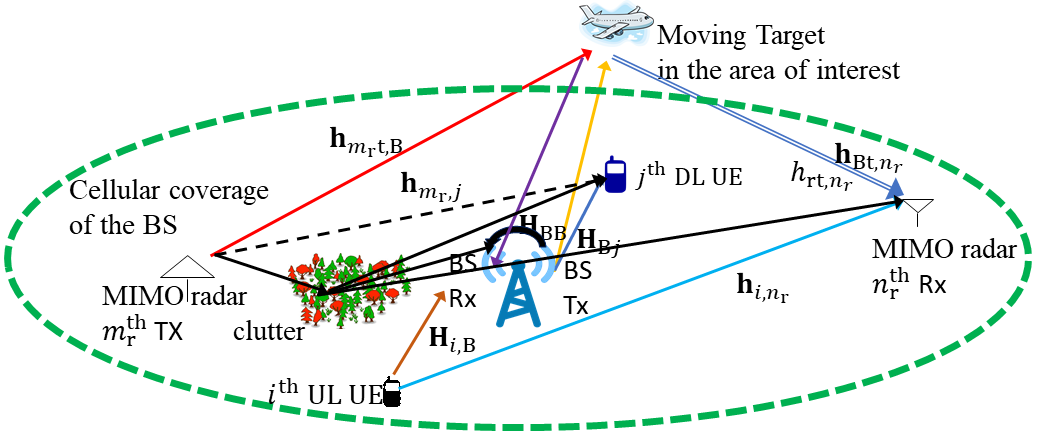
\includegraphics[width=1\columnwidth]{setup_model_tsp.png}
		%\vspace{-pt}
		\caption{Co-design system model comprising a statistical (widely distributed) MIMO radar and IBFD MU-MIMO communications.}
		\label{fig:setup}
		%\vspace{-1em}
	\end{figure}
	\textcolor{red}{We consider a spectral co-design for a statistical MIMO radar and an IBFD MU-MIMO communications system occupying the same spectrum.} As shown in \figurename{~\ref{fig:setup}}, the $M_\mathrm{r}$ Txs and $N_\mathrm{r}$ Rxs of the statistical MIMO radar are located on a 2-D plane $\left(x,y \right)$ along with the BS, $I$ UL UEs and $J$ DL UEs of the IBFD MU-MIMO communications system at coordinates $\left(x_{m_\mathrm{r}},y_{m_\mathrm{r}}\right)$, $\left(x_{n_\mathrm{r}},y_{n_\mathrm{r}} \right)$,  $\paren{x_{\mathrm{B}},y_{\mathrm{B}}}$, $\paren{x_{\mathrm{UL},i},y_{\mathrm{UL},i}}$, and $\paren{x_{\mathrm{DL,}j},y_{\mathrm{DL},j}}$, respectively, for all $m_\mathrm{r}\in{Z}_{+}(M_\mathrm{r})$, $n_\mathrm{r}\in\mathbb{Z}_{+}\paren{N_\mathrm{r}}$, $i\in\mathbb{Z}_{+}\paren{I}$, and $j\in\mathbb{Z}_{+}\paren{J}$. The goal of the statistical MIMO radar is to detect a moving target located at $(x_{\mathrm{t}},y_{\mathrm{t}})$ that is coterminous with the cellular coverage of the BS while the IBFD MU-MIMO communications system aims to serve the UL/DL UEs with desired achievable rates despite the presence of the radar probing signals.  %\textcolor{red}{Why is this in Roman numerals. It should also be Fig. 1}. 
	%In the sequel, we describe the system models of each of these units in detail and then present the co-design formulation.
	\subsection{Transmit Signal Model}
	We base our spectral co-design model on an observation window shown in \figurename{\;\ref{fig:transmissionmodel}}, where each radar Tx emits a pulse train of $\mathit{K}$ pulses within a \textit{coherent processing interval} (CPI) while the BS and each UL UE continuously transmit DL and UL symbols, respectively. The time between  pulses is denoted as the pulse repetition interval (PRI) with duration $T_{\mathrm{r}}$, which leads to the the length of the CPI as $KT_{\mathrm{r}}$. The pulse width is $T_\mathrm{p}= T_\mathrm{r}/N$, where $N$ denotes the number of range cells in a PRI. The $\mathit{K}$ is chosen such that the range migration does not occur for the duration of the pulse train\cite{Xiaodong_Overlaid}.
	As we co-design the radar and FD communications systems, the radar pulse width $T_{\mathrm{p}}$ equals the UL/DL symbol period.  
	The UL and DL transmissions are fully synchronized in the time domain because the BS operates on the FD mode. The transmissions of the MIMO radar and the FD MU-MIMO communications are asynchronous with the delay between the beginning of the . Without loss of generality, we assume that the beginning of the $\ith{k}$ frame of the  
	\color{red}We propose a JRC model without requiring synchronous radar and communications transmissions and the . Specifically, we assume that the time interval between the beginning of the $\ith{m}$ frame and the $\ith{k}$ PRI is $GT_{\mathrm{p}}$, where $G\in\mathbb{Z}_\braces{N-1}$.  To The clocks at the BS and the MIMO radar are offline synchronized and periodically maintained using a certain clock synchronization protocol, such as the IEEE 1588 precision time protocol\cite{wang2020displaced} such that the clock offset between the BS and MIMO radar Rxs is negligible. The UL UEs clock information is also readily available at the radar Rxs through the feedback from the BS. As the FD MU-MIMO communications is also assumed to be synchronized, the UL UEs and  
	\color{black}Further, the length of a UL/DL frame $T_\mathrm{f}$ is identical to the radar PRI, i.e., $T_{\mathrm{f}}=T_{\mathrm{r}}$ and the UL/DL symbol duration $T_{\mathrm{s}}$ is equal to the radar pulse width $T_{\mathrm{p}}$, i.e., $T_{\mathrm{s}}=T_{\mathrm{p}}$, which alludes that the number of UL/DL frames transmitted in the scheduling window is also $\mathit{K}$ and the number of UL/DL symbols in each frame is $\sfrac{T_{\mathrm{f}}}{T_{\mathrm{s}}}=\mathit{N}$. The symbol level synchronization is assumed here. The range cell and the communications symbols are synchronized. The communications symbols and the radar range cells are aligned because of the same sampling rate employed by the JRC system.
	\begin{figure}[!t]
		%\begin{figure*}[!t]
		\centering
		%	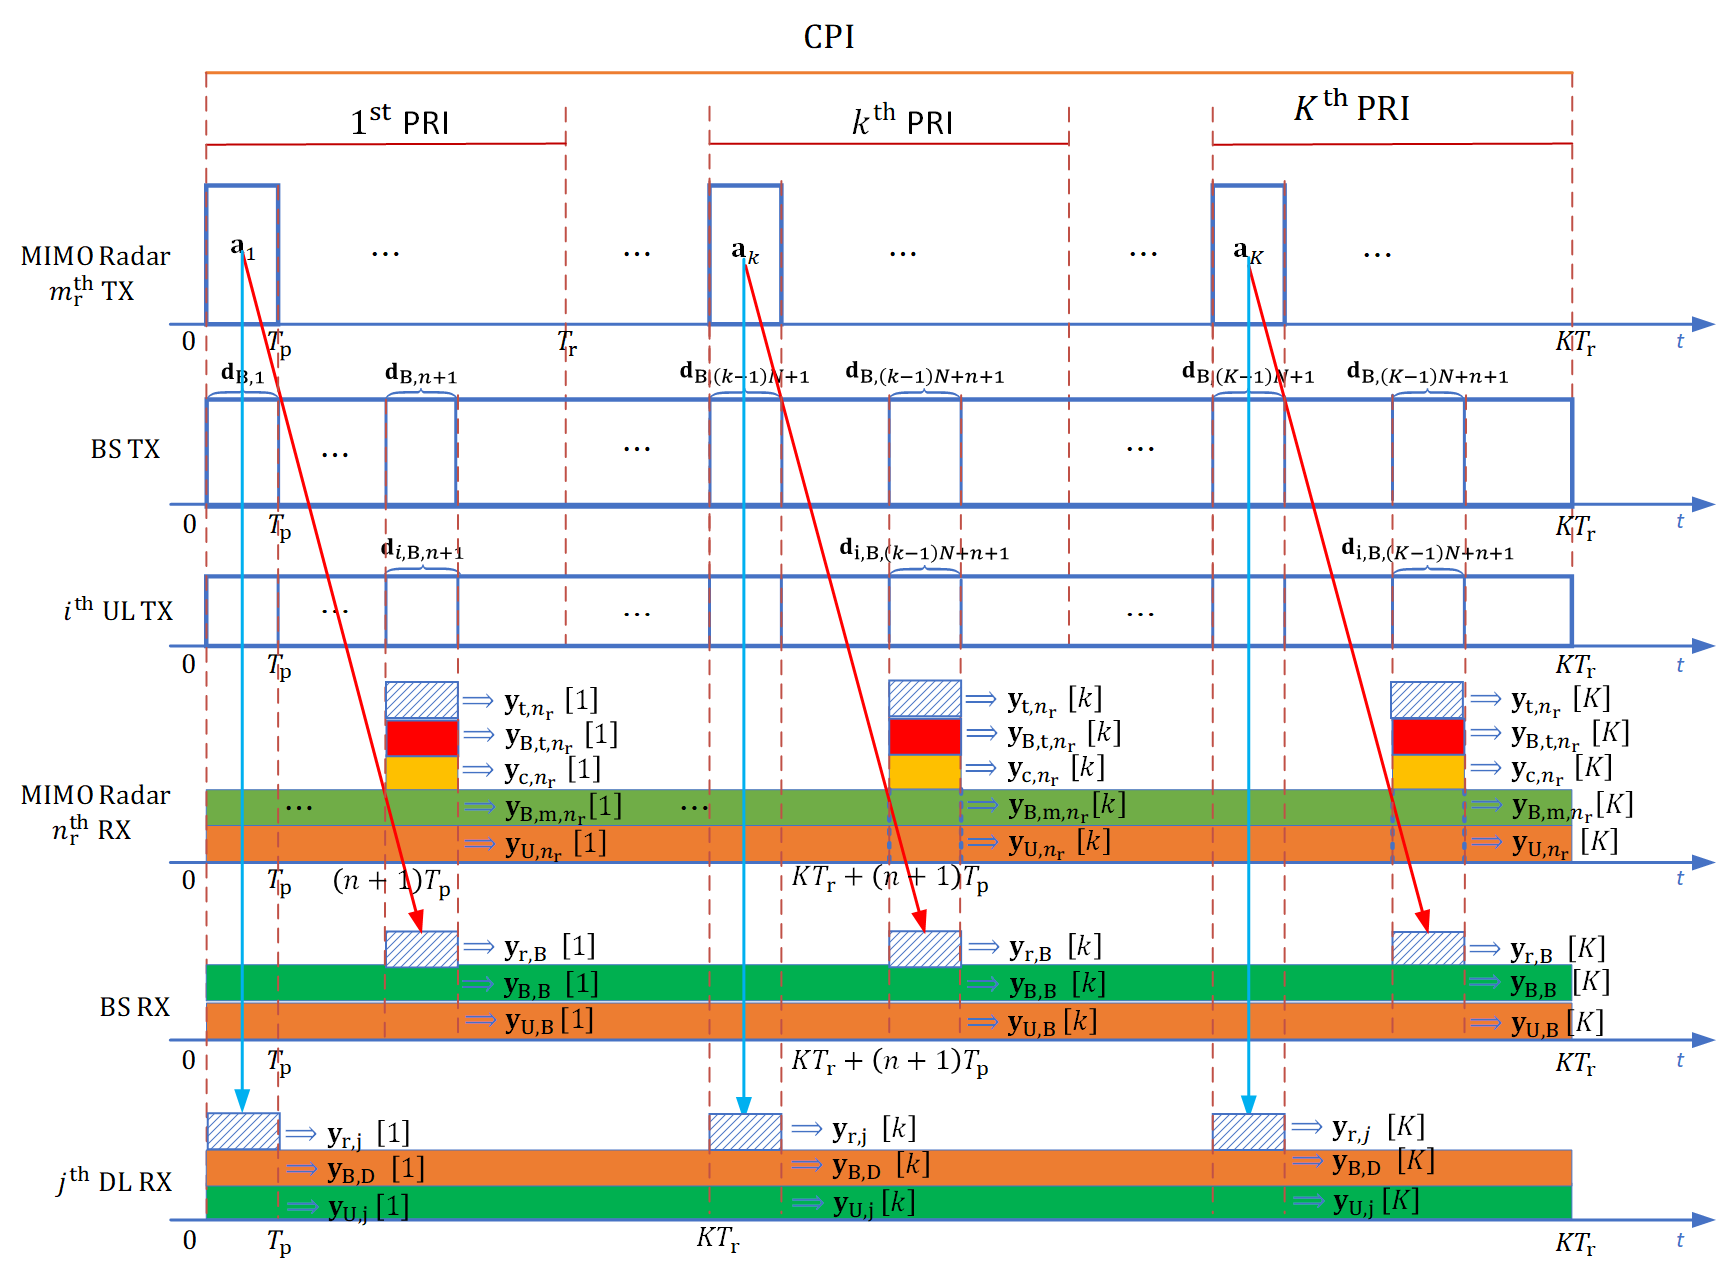
\includegraphics[width=3.1in]{Drawing3}
		%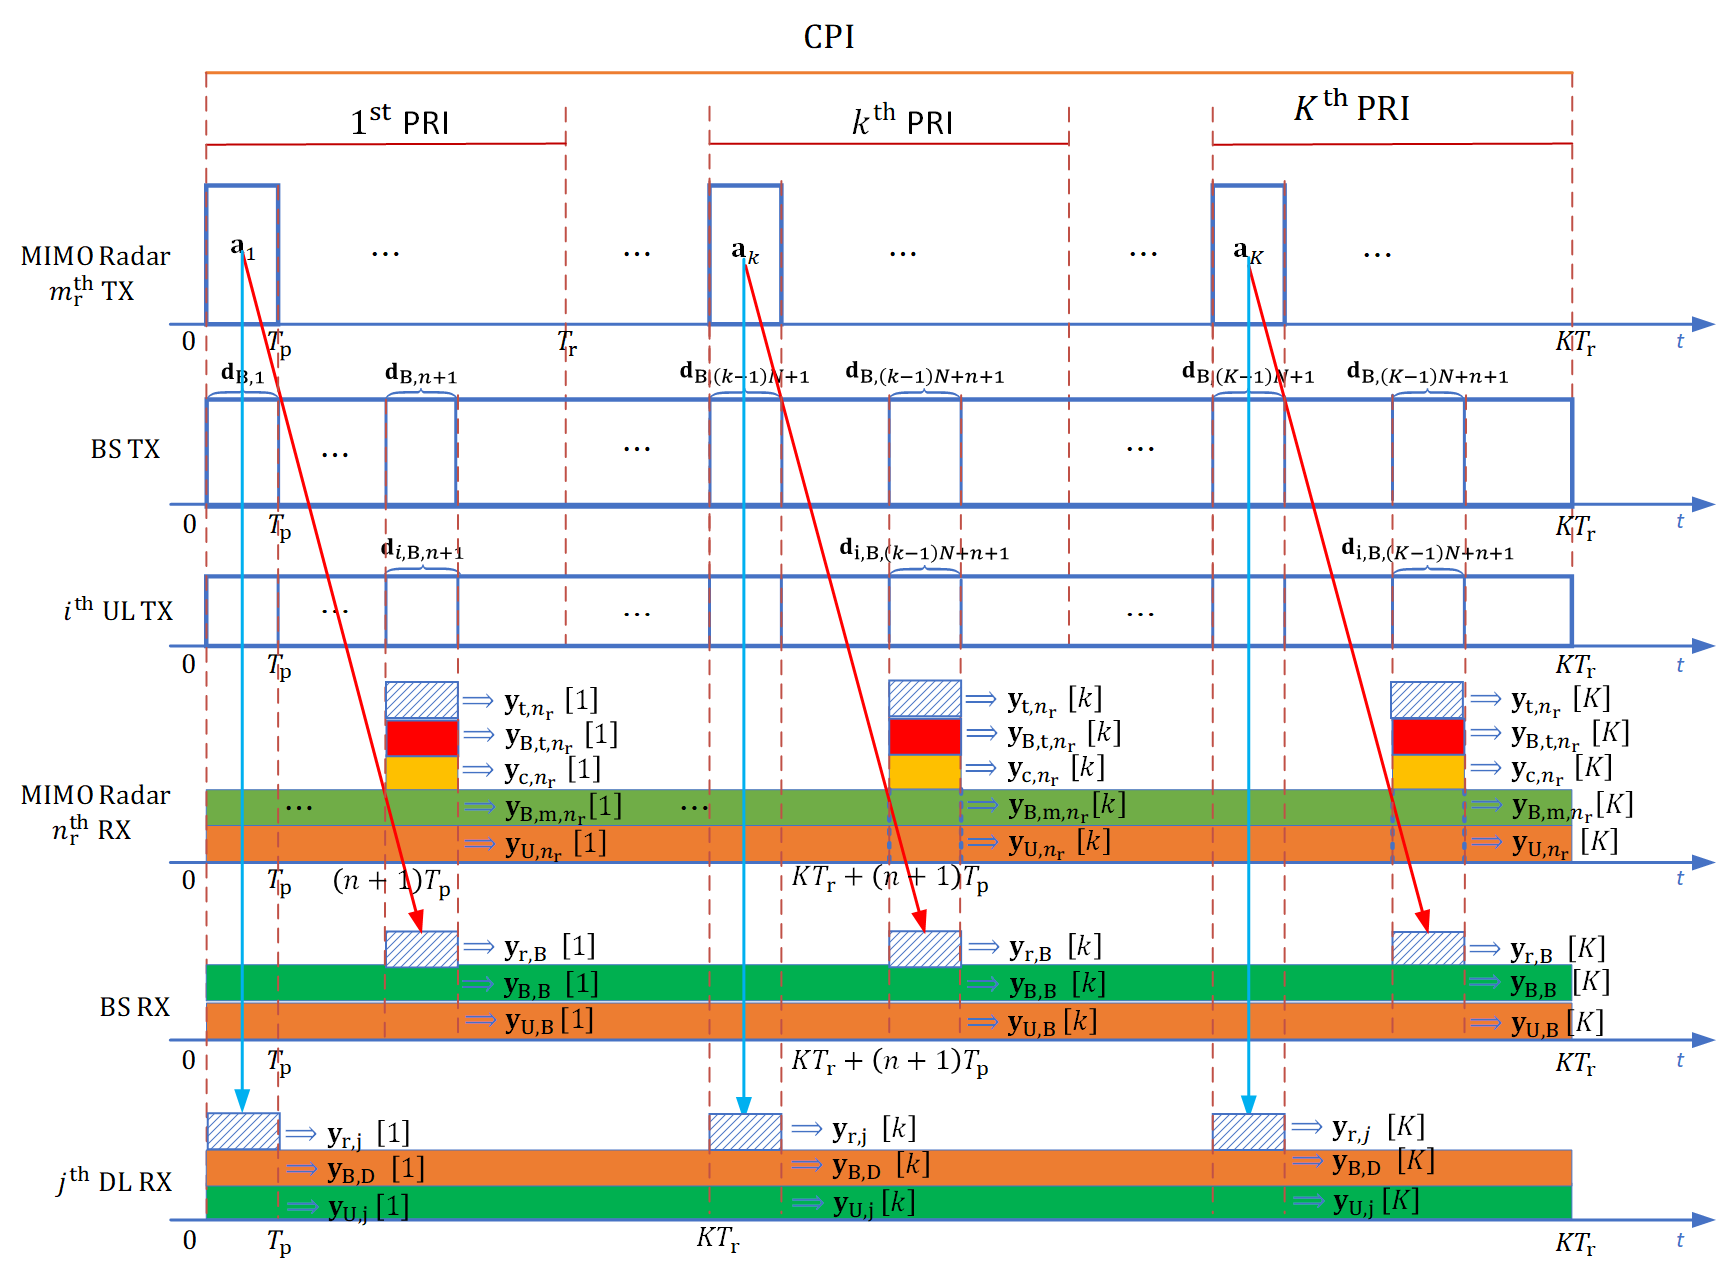
\includegraphics[width=0.80\textwidth]{Drawing3.png}
		%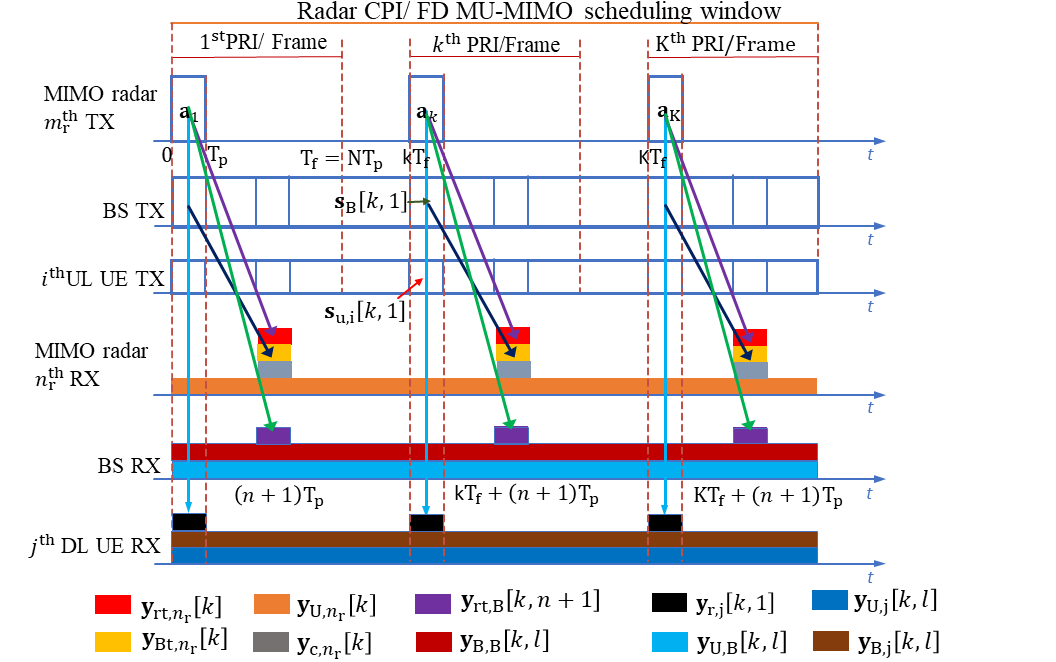
\includegraphics[width=0.80\textwidth]{systemmodel.png}
		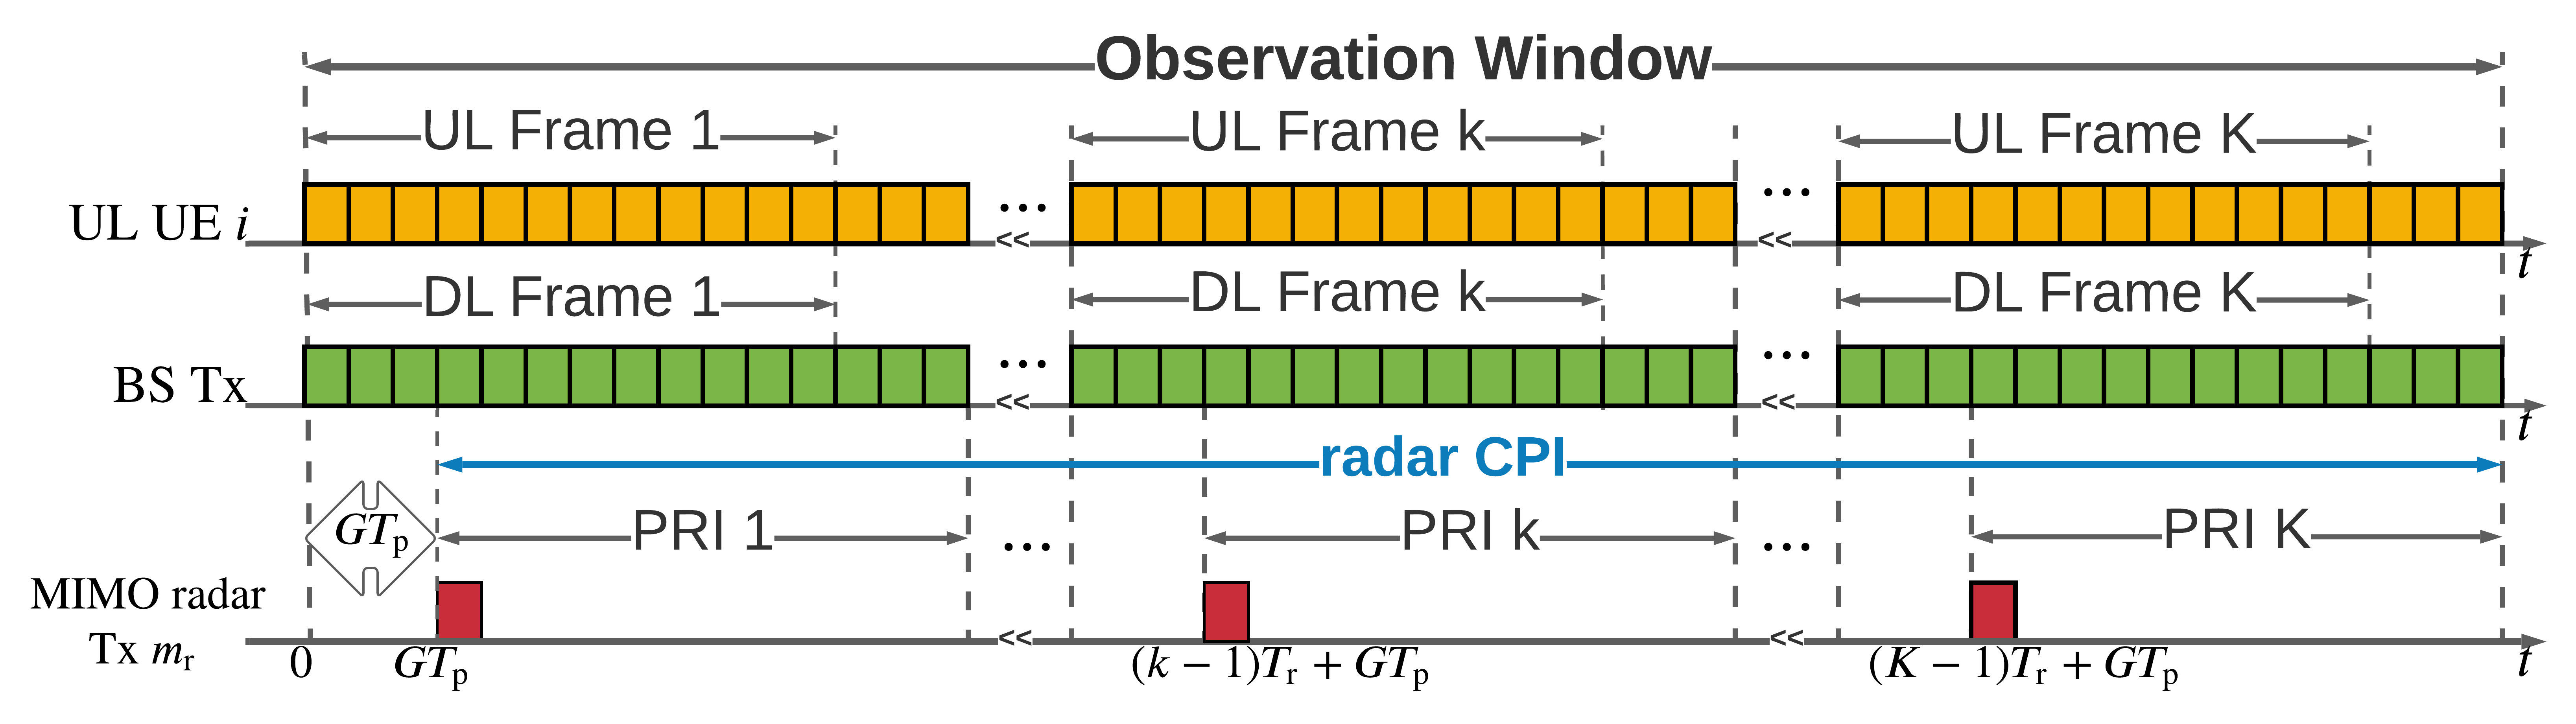
\includegraphics[width=1.0\columnwidth]{newFigures/Transmission.png}
		\caption{\textcolor{red}{The time-domain observation window spans across $t\in\bracket{0,KT_{\mathrm{r}}+GT_\mathrm{p}}$, where each bin represents a radar pulse or a communications symbol with length $T_{\mathrm{p}}$. Within the observation window, the communications data transmissions occur continuously while pulsed radar Txs emit probing signals intermittently during the radar CPI.}
			%For each MIMO radar Rx, we focus on the $\ith{n}$ range cell where the target is observed. The $\ith{j}$ UE is interfered by the radar probing signal during the symbol period when the MIMO radar transmits pulses. %\textcolor{red}{\textbf{The top text is cut off.}}
		} 
		%\vspace{-2em}
		\label{fig:transmissionmodel}
	\end{figure} %Recall our discussion prior to 
	%\vspace{-1em}
	\subsubsection{Statistical MIMO Radar Transmit Signal Model}
	%which consists of a statistical MIMO radar composed of $M_\mathrm{r}$ transmitters (Tx) and $N_\mathrm{r}$ receivers (Rx), a communications BS equipped with $M_\mathrm{c}$ antennas and $\mathit{J}$ active user equipment (UEs), where each UE $\mathit{J}$ is equipped with $\mathit{N}_{\mathrm{d},j}$ transmit/receive antennas for all $j\in\mathbb{Z}_{+}(J)$. 
	% \subsubsection{MIMO Radar Model}\label{mimoradarsys}
	%The $M_\mathrm{r}$ Tx and $N_\mathrm{r}$ Rx of the MIMO radar as well as the BS and the $N$ UEs are located in a 2-D plane $\left(x,y \right)$ at coordinates $\left(x_{m_\mathrm{r}},y_{m_\mathrm{r}}\right)$, $m_\mathrm{r}\in{Z}_{+}(M_\mathrm{r})$ and $\left(x_{n_\mathrm{r}},y_{n_\mathrm{r}} \right)$, $n_\mathrm{r}\in\mathbb{Z}_{+}(N_\mathrm{r})$, as well as $(x_{\textrm{B}},y_{\textrm{B}})$ and $(x_{\mathrm{n}},y_{\mathrm{n}})$, $n\in\mathbb{Z}_{+}(N)$, respectively. 
	%The statistical MIMO radar is composed of $\mathit{M}_\textrm{r}$ single antenna Txs and $\mathit{N}_\mathrm{r}$ Rxs. 
	
	%\textcolor{red}{Should be $\mathbf{a}_{m_r}$? Or this is same for each Tx? Why its length depends on the number of Tx?}. 
	Denote $a_{m\rr,k}$ as the radar code to modulate the pulse emitted by the radar Tx $m\rr$ in the $\ith{k}$ PRI. Based on the transmission model, the pulse train transmitted by the $\ith{m_\mathrm{r}}$ Tx within the observation window is given as
	\par\noindent\small
	\begin{IEEEeqnarray}{rCl}
		s_{m_\mathrm{r}}\paren{t}=\sum_{k=1}^{\mathit{K}}a_{m_\mathrm{r},k}\phi_{m_\mathrm{r}}\paren{t-\paren{k-1}T\rr-GT_{\mathrm{p}}},
	\end{IEEEeqnarray}\normalsize 
	where $t\in\bracket{0,KT\rr+GT_{\mathrm{p}}}$, $\phi_{m_\mathrm{r}}\paren{t}$ denotes the pulse waveform transmitted by the radar Tx $m\rr$, which is also 
	%$\tau \in\left[0,T_\textrm{B} \right)$, $k\in \mathbb{Z}(K)$, and $l_\mathrm{s}\in \mathbb{Z}^+(L_\mathrm{s})$ denote the radar Tx antenna index, the fast time, i.e., the time index within one pulse, the slow time, i.e., the index of radar pulse, and the subpulse index, respectively,
	the $\ith{m_\mathrm{r}}$ element of the  \textit{narrowband} radar transmit waveform vector $\boldsymbol{\phi}(t)=\left[ \phi_1(t),\dots,\phi_{M_\mathrm{r}}(t)\right]^\top\in\mathbb{C}^{M\rr}$ with the orthonormality condition $\int_{T_\mathrm{p}}^{}\boldsymbol{\phi}(t)\boldsymbol{\phi}^\dagger(t)dt=\mathbf{I}_{M_\mathrm{r}}$. The total MIMO radar code matrix is defined as $\mathbf{A}=\bracket{\mathbf{a}^\top\bracket{1};\cdots; \mathbf{a}^\top\bracket{\mathrm{\mathit{K}}}}\in\mathbb{C}^{\mathit{K}\times \mathit{M}\rr}$, where $\mathbf{a}\bracket{k}=\bracket{a_{1,k},\cdots,a_{\mathit{M}\rr,k}}^\top\in\mathbb{C}^{M\rr}$ is the radar code vector transmitted during the $\ith{k}$ PRI.  The total transmit signal vector is defined as $\mathbf{s}(t)=\bracket{s_1(t),\cdots,s_{M_\mathrm{r}}(t)}^\top\in\mathbb{C}^{M\rr}$. 
	
	%We first generalize the extended target model developed in the conventional MIMO radar research \cite{MIMOradarseparatedantennas,target_localization,widely_extendedtarget} to facilitate the co-design of MIMO radar and communications system. 
	%We consider a far-field scenario where the target scenario has an extended target composed of a large number of independent point-like scatterers. %In contrast to a far-field target, the distance and angle of a near-field target is a function of the transmit and receive element locations as well as the location of the individual scatterer\cite{fisher2006MIMO,haimovich2008mimo}. However, due to the central limit theorem and narrowband transmit signal assumption, 
	\subsubsection{IBFD MU-MIMO Communications Transmit Signal Models}
	For the IBFD MU-MIMO communications system, the BS operates on the FD mode and the UEs on the HD mode.  During the observation window, the BS receives data frames from the $I$ UL UEs and the $J$ DL UEs download data frames from the BS simultaneously on the same band. The BS is equipped with $\mathit{M}_\mathrm{c}$ transmit and $\mathit{N}_{\mathrm{c}}$ receive antennas. The UL UE $i$ and the DL UE $j$ employ $\mathit{N}_{\mathrm{u},i}$ and $\mathit{N}_{\mathrm{d},j}$ transceiving antennas, respectively. To achieve the maximum capacities of the UL and DL channels indicates $\mathit{M}\cc\geq\sum_{j=1}^{\mathit{J}}\mathit{N}_{\textrm{d},j}$ and $\mathit{N}\cc\geq\sum_{i=1}^{\mathit{I}}\mathit{N}_{\textrm{u},i}$\cite{tse2005fundamentals}. % for all $\braces{i}$ and $\braces{j}$ %$j\in\mathbb{Z}_{+}(\mathit{J})$. 
	The number of unit-energy data streams used by the UL UE $i$ and the DL UE $j$ are $\mathrm{D}_{\textrm{u},i}\leq \mathit{N}_{\mathrm{u},i}$ and $\mathit{D}_{\mathrm{d},j}\leq \mathit{N}_{\mathrm{d},j}$, respectively. We denote the symbol vectors sent by the UL UE $i$ toward the BS and by the BS toward the DL UE $j$ in the  $\ith{l}$ symbol period of the $\ith{m}$ frame by $\mathbf{d}_{\mathrm{u},i}\bracket{m,l}\in \mathbb{C}^{D_{\textrm{u},i}}$ and $\mathbf{d}_{\mathrm{d},j}\bracket{m,l}\in \mathbb{C}^{\mathit{D}_{\mathrm{d},j}}$, respectively, which are independent and identically distributed (i.i.d.) for $i\in\mathbb{Z}_+\braces{\mathit{I}}$, $m\in\mathbb{Z}_+\braces{\mathit{M}}$, and $l\in\mathbb{Z}_+\braces{\mathit{N}}$. 
	Denote the precoders for the UL UE $i$ and the DL UE $j$ at the $\ith{k}$ frame as $\PiB\in\mathbb{C}^{\mathit{N}_{\mathrm{u},i}\times \mathit{D}_{\mathrm{u},i}}$ and $\PBj\in\mathbb{C}^{\mathit{M}\cc\times \mathit{D}_{\mathrm{d},j}}$, respectively, the symbol vectors for the UL UE $i$ and DL UE $j$ at the $\ith{l}$ symbol period of the $\ith{k}$ frame are formed as $\mathbf{s}_{\textrm{u},i}\bracket{m,l}=\PiB\mathbf{d}_{\mathrm{u},i}\bracket{m,l}$ and $\mathbf{s}_{\textrm{d},j}\bracket{m,l}=\PBj\mathbf{d}_{\mathrm{d},j}\bracket{m,l}$, respectively. \color{red}We can then show the composite transmitted signals of the UL UE $i$ and the BS as\par\noindent\small
	\begin{equation}
		\mathbf{x}_{\mathrm{u},i}\paren{t}=\sum_{\kappa}^{}\sum_{l=0}^{N-1}\mathbf{s}_{\mathrm{u},i}\bracket{m,l}p_{\mathrm{T}}\paren{t-(kN+l)T_{\mathrm{p}}},    
	\end{equation}
	\normalsize
	\par\noindent\small
	\begin{flalign}
		\mathbf{x}_{\mathrm{B}}\paren{t}=&\sum_{j=1}^J\sum_{\kappa=0}^{K-1}\sum_{\ell=0}^{N-1}\mathbf{s}_{\mathrm{d}
			,j}\bracket{\kappa,\ell}p_{\mathrm{T}}\paren{t-\paren{\kappa N+\ell}T_{\mathrm{p}}}
	\end{flalign}
	\normalsize
	where $p_{\mathrm{T}}$ is the transmit pulse shaping function employed by the FD communications system and whose discrete-time versions are given as $\mathbf{x}_{\mathrm{u},i}\bracket{n}\triangleq\mathbf{x}_{\mathrm{u},i}\paren{nT_\mathrm{p}}$ and $\mathbf{x}_{\mathrm{B}}\bracket{n}\triangleq\mathbf{x}_{\mathrm{B}}\paren{nT_\mathrm{p}}$.
	
	%$\mathbf{d}_{\mathrm{d},j}\bracket{m,l}$ is also unit-energy, i.e., $\mathbb{E}\bracket{\mathbf{d}_{\mathrm{d},j}\bracket{m,l}\mathbf{d}^\dagger_{\textrm{B},j}\bracket{m,l}}=\mathbf{I}_{\mathit{N}_{\mathrm{d},j}}$ \cite{Gasussianduality}. %A complex precoding matrix is assigned to each UE to achieve multiple-access interference suppression and spatial diversity exploitation\cite{ArraytoMIMO,ShiftMIMO}. 
	\color{black}
	\subsection{Spectral Co-design Channel Models}
	\subsubsection{Statistical MIMO Radar Channel Model} 
	The complex reflectivity of the point target corresponding to the $\ith{m\rr}$ Tx - $\ith{n\rr}$ Rx path is modeled as a CSCG random variable $\alpha_{m\rr \target n\rr }\sim\mathcal{CN}(0,\eta^2_{m\rr\target n\rr})$, where $\eta^2_{m\rr\textrm{t}n\rr}$ denotes the average reflection power of the point target proportional to the target RCS\cite{NaghshTSP2017}; it remains constant over the CPI as per the Swerling I (block fading) target model \cite{haimovich2008mimo}. %Collect the target reflectivities with respect to all Txs observed at the $\ith{n\rr}$ radar Rx in a vector $\mathbf{h}_{\textrm{rt,}n\rr}\triangleq\bracket{h_{1\textrm{t}n\rr},\cdots,h_{M\rr\textrm{t}n\rr}}^\top\in\mathbb{C}^{M\rr}$. 
	
	%Furthermore, the waveforms $\braces{\boldsymbol{\phi}(t)}_{m\rr=1}^{\mathit{M}\rr}$ are narrowband. \cite{MIMOradarseparatedantennas,spacetimecodemimo,MCMIMO_Rad,target_localization}
	%Assume that the coverage of this statistical MIMO radar has a moving target, which is characterized by ts complex reflectivity, location \textcolor{red}{all details related to the location also removed?}, and Doppler velocity \textcolor{red}{You have removed all the previous details that connected the velocity to frequency. Those details are needed.}. The complex reflectivity of the target with respect to the $\ith{m\rr}$ Tx - $\ith{n\rr}$ Rx pair is specified by a CSCG random variable $\alpha_{m\rr \target n\rr }\sim\mathcal{CN}(0,\eta^2_{\target})$, where $\eta^2_{\target}$ \textcolor{red}{Why is this power not dependent on the specific Tx-Rx path chosen?} denotes the average reflection power of the target and is considered constant over the CPI \cite{sun2019target}. The Doppler frequency of the target with respect to the same $\ith{m\rr}$ Tx - $\ith{n\rr}$ Rx pair is $f^\prime_{m_\mathrm{r}\target n_\mathrm{r}}$ that we normalize by the PRI as $f_{m_\mathrm{r}\target n_\mathrm{r}}= f^\prime_{m_\mathrm{r}\target n_\mathrm{r}}\mathit{T}\rr$\cite{hongbin_movingtarget}. The motion of the target is slow enough such that $f_{m_\mathrm{r}\target n_\mathrm{r}}T\rr$ remains constant within each pulse. %and fluctuates from pulse to pulse. 
	
	%\textcolor{red}{No mention of analog signal, downconversion, sampling? These are very important details.} 
	The velocity of the target is the vector  $\boldsymbol{\nu}_{t}\triangleq\left(\nu_\mathrm{\mathrm{x},t},\nu_\mathrm{\mathrm{y},t} \right)$, where $\nu_\mathrm{\mathrm{x},t}$ and $\nu_\mathrm{\mathrm{y},t}$ are deterministic but unknown horizontal and vertical velocity components in the 2-D plane. The Doppler frequency with respect to the $\ith{m\rr}$ Tx - $\ith{n\rr}$ Rx pair is $f_{m_\mathrm{r}\target n_\mathrm{r}} = \frac{\nu_\mathrm{\mathrm{x},t}}{\lambda}(\cos\theta_{m_\mathrm{r}\target}+\cos\phi_{n_\mathrm{r}\target})+\frac{\nu_\mathrm{\mathrm{y},\target}}{\lambda}(\sin\theta_{m_\mathrm{r}\target}+\sin\phi_{n_\mathrm{r}\target})$ \cite{hongbin_movingtarget},
	\iffalse
	\par\noindent\small
	\begin{IEEEeqnarray}{rCl}
		%\begin{IEEEeqnarray}{rCl} 
		%\IEEEyesnumber\IEEEyessubnumber*
		f_{m_\mathrm{r}\target n_\mathrm{r}} &=& \frac{\nu_\mathrm{\mathrm{x},t}}{\lambda}(\cos\theta_{m_\mathrm{r}\target}+\cos\phi_{n_\mathrm{r}\target})\nonumber\\
		&&+\frac{\nu_\mathrm{\mathrm{y},\target}}{\lambda}(\sin\theta_{m_\mathrm{r}\target}+\sin\phi_{n_\mathrm{r}\target}) \nonumber  \label{normalized doppler}
		%\end{IEEEeqnarray}
	\end{IEEEeqnarray}\normalsize
	\fi
	where $\lambda$ denotes the carrier wavelength, $\theta_{m_\mathrm{r}}$ and $\phi_{n_\mathrm{r}}$ are the angles of departure at the $\ith{m_\mathrm{r}}$ Tx and angles of arrival at the $\ith{n_\mathrm{r}}$ Rx, respectively. %, with respect to the target. 
	The narrowband assumption of $s_{m\rr}(t)$ allows us to approximate the propagation delay arising from the reflection off an arbitrary scatterer of the $\ith{n_\mathrm{r}}$ extended target to that from the center of gravity of the $\ith{n_\mathrm{r}}$ extended target, for all $m_\mathrm{r}\in\mathbb{Z}_{+}(M_\mathrm{r})$ and $n_\mathrm{r}\in\mathbb{Z}_{+}(N_\mathrm{r})$\cite{haimovich2008mimo}. If center of gravity of the extended target is $(x_{t},y_{t})$, then the the propagation delay with respect to $\ith{m\rr}$ Tx - $\ith{n\rr}$ Rx  is
	$\zeta_{m\rr \target n\rr}=\frac{\sqrt{\paren{x_{m\rr}-x_{t}}^2+\paren{y_{m\rr}-y_{t}}^2}}{c}
	+\frac{\sqrt{\paren{x_{n\rr}-x_{t}}^2+\paren{y_{n\rr}-y_{t}}^2}}{c},$
	\iffalse
	\par\noindent\small
	\begin{IEEEeqnarray}{rCl}
		\zeta_{m\rr \target n\rr }&=&\frac{\sqrt{\paren{x_{m\rr}-x_{t}}^2+\paren{y_{m\rr}-y_{t}}^2}}{c}\nonumber\\
		&&+\frac{\sqrt{\paren{x_{n\rr}-x_{t}}^2+\paren{y_{n\rr}-y_{t}}^2}}{c}\nonumber
	\end{IEEEeqnarray} \normalsize
	\fi
	where $c=3\times 10^8$ m/s is the speed of the light. The slow-motion assumption of the target guarantees that $\zeta_{m\rr \target n\rr }$ is constant during each CPI. %, which further infers that the target remains in the same range cell over the entire CPI\cite{fisher2006MIMO}. 
	\subsubsection{IBFD MU-MIMO Communications Channel Models}
	Denote the UL channel from the $\ith{i}$ UL UE to the BS and the DL channel between the BS and the $\ith{j}$ DL UE as  $\mathbf{H}_{i,\textrm{B}}\in\mathbb{C}^{\mathit{M}\cc\times \mathit{N}_{\mathrm{u},i}}$ and $\mathbf{H}_{\textrm{B},j}\in\mathbb{C}^{\mathit{N}_{\mathrm{d},j}\times \mathit{M}\cc}$, which are full rank for all $i$ and $j$ to achieve the highest spatial degrees of freedom of the MIMO channels \cite{tse2005fundamentals}.  
	The FD architecture of the BS implies that the BS Rx receives DL signals through the self-interfering channel $\mathbf{H}_{\mathrm{BB}}\in{\mathbb{C}^{\mathit{N}\cc\times \mathit{M}\cc}}$. Meanwhile, the UL signals simultaneously radiated by the $I$ UL UEs interfere with the DL UE $j$ via the channel $\mathbf{H}_{i,j}\in\mathbb{C}^{\mathit{N}_{\mathrm{d},j}\times \mathit{N}_{\mathrm{u},i}}$. The elements of $\mathbf{H}_{\textrm{B},j}$, $\mathbf{H}_{i,\textrm{B}}$, $\mathbf{H}_{i,j}$, and $\mathbf{H}_{\textrm{B,B}}$ are random variables (RVs) distributed as $\mathcal{CN}\paren{0,\eta^2_{\textrm{d},j}}$, $\mathcal{CN}\paren{0,\eta^2_{\textrm{u},i}}$, $\mathcal{CN}\paren{0,\eta^2_{i,j}}$, and $\mathcal{CN}\paren{0,\eta^2_{\textrm{BB}}}$, respectively, for all $i$ and $j$. Assume perfect CSI at the Tx and Rx (CSITR) is available to the IBFD MU-MIMO communications as well as the MIMO  radar.
	\color{red}
	\subsubsection{Joint Radar-Communications Channel Models}
	The proposed radar-communications co-design model exploits the DL signals to aid the radar target detection by enabling a cooperative DL-radar mode. 
	We suppose that the moving target remains in the illumination region of the BS during the CPI. The DL signals arrive at the $\ith{n\rr}$ MIMO radar Rx via a direct path and a target reflection path, whose CIRs are modeled as $\mathbf{h}_{\mathrm{Bm},n\rr}\in\mathbb{C}^{M\cc}$ and the target reflection path $\mathbf{h}_{\mathrm{Bt,}n\rr}\in\mathbb{C}^{M\cc}$,
	which are respectively modeled as,
	\par\noindent\small
	\begin{flalign}
		\mathbf{h}_{\mathrm{Bm},n\rr}\paren{t,\tau}=&h_{\mathrm{Bm},n\rr}\mathbf{a}_{\mathrm{T}}^\dagger\paren{\theta_{\mathrm{B},n\rr}}e^{j2\pi f_{\mathrm{Bm},n\rr}t}\delta\paren{\tau-\tau_{\mathrm{Bm},n\rr}}\nonumber
	\end{flalign}
	\begin{flalign}
		\text{and\;}\mathbf{h}_{\mathrm{Bt},n\rr}\paren{t,\tau}=&\alpha_{\mathrm{B\target},,n\rr}\mathbf{a}_{\mathrm{T}}^\dagger\paren{\theta_{\mathrm{B},\target}}e^{j2\pi f_{\mathrm{B\target},n\rr}t}\delta\paren{\tau-\tau_{\mathrm{B\target},,n\rr}}\nonumber
	\end{flalign}
	\normalsize 
	where $\theta_{\mathrm{B},n\rr}$ and $\theta_{\mathrm{B},\target}$ are the the angles of departure (AoDs) at the BS w.r.t the path between the BS and the $\ith{n\rr}$ radar Rx and the path between the BS and the target with $\mathbf{a}_{\mathrm{T}}^\dagger\paren{\theta_{\mathrm{B},n\rr}}$ and $\mathbf{a}_{\mathrm{T}}^\dagger\paren{\theta_{\mathrm{B},\target}}$ being their corresponding transmit steering vectors; $\tau_{\mathrm{B},n\rr}$ and $f_{\mathrm{B},n\rr}$ the channel path gain, delay and Doppler shift of the direct path, respectively; and $\alpha_{\mathrm{Bt},n\rr}$, $\tau_{\mathrm{Bt},n\rr}$, $f_{\mathrm{Bt},n\rr}$ the channel path gain, delay and Doppler shift of the path: BS $\rightarrow$ target $\rightarrow$ radar Rx $n\rr$, respectively. 
	
	Next, we model the channels for signals radiated by the radar Tx arriving at the BS and the $\ith{j}$ DL UE as 
	\par\noindent\small
	\begin{IEEEeqnarray}{rCl}
		\IEEEyessubnumber*
		\mathbf{h}_{m\rr,\mathrm{B}}\paren{t,\tau}&=&\alpha_{m\rr\target\mathrm{B}}\mathbf{a}_\mathrm{R}\paren{\theta_{\target,\mathrm{B}}}e^{j2\pi f_{m\rr\target\mathrm{B}}t}\sigma_{\mathrm{r}}\paren{\tau-\tau_{m\rr\target\mathrm{B}}}\label{eq: radar_t_BS_channel}\\
		&&+\alpha_{m\rr,\mathrm{B}}\mathbf{a}_\mathrm{R}\paren{\theta_{m\rr,\mathrm{B}}}e^{j2\pi f_{m\rr,\mathrm{B}}t}\sigma_{\mathrm{r}}\paren{\tau-\tau_{m\rr\mathrm{B}}}\label{eq: radar_BS_channel}  
	\end{IEEEeqnarray}
	\normalsize
	\par\noindent\small
	\begin{flalign}
		\label{eq: radar_DL_channel}
		\text{and\;}\mathbf{h}_{m\rr,j}\paren{t,\tau}=&\alpha_{m\rr,n_{\target},j}\mathbf{a}_\mathrm{R}\paren{\theta_{\target,j}}e^{j2\pi f_{m\rr,\target,j}t}\sigma\paren{t-\tau_{m\rr,\target,j}},
	\end{flalign}\normalsize
	respectively, where the RHS of $\paren{\ref{eq: radar_t_BS_channel}}$ and the RHS of $\paren{\ref{eq: radar_BS_channel}}$ represent the target reflection path and the direct path for the DL signals to reach the BS; $\mathbf{a}_\mathrm{R}\paren{\theta_{\target,\mathrm{B}}}$, $\mathbf{a}_\mathrm{R}\paren{\theta_{m\rr,\mathrm{B}}}$ and $\mathbf{a}_{\mathrm{R}}\paren{\theta_{\target,j}}$, are the receive steering vectors w.r.t the angle of arrivals (AoAs) $\theta_{{\target},\mathrm{B}}$ between the target and the BS $j$, $\theta_{m\rr,\mathrm{B}}$ between the $\ith{m\rr}$ radar Tx and BS and the DL UE $j$ as well as  $\theta_{\target,j}$ between the target and the DL UE $j$; $h_{m\rr,n_{\target},j}$, $f_{m\rr,n_{\target},j}$, and $\tau_{m\rr,n_{\target},j}$ denote the complex gain, Doppler shift, and delay for the path: radar Tx $m\rr$ $\rightarrow$ target $n_{\target}$ $\rightarrow$ DL UE $j$, respectively.
	We do not consider the target reflection path in $\paren{\ref{eq: radar_DL_channel}}$
	because of the relatively small effective antenna apertures of the DL UEs compared to the BS, which hinders the DL UEs to distinguish the radar signals scattered off the target from the background noise.
	
	\color{black}
	A similar argument above can be made about the UL signals arrive at the radar $n\rr$ via only the direct path because of the smaller antenna aperture of UL UEs. The CIR between the UE $i$ and the radar Rx $n\rr$ is modeled as
	\par\noindent\small
	\begin{flalign}
		\mathbf{h}_{i,n\rr}\paren{t,\tau}=\alpha_{i,n\rr}\mathbf{a}_{\mathrm{T}}^\dagger\paren{\theta_{i,n\rr}}e^{j2\pi f_{i,n\rr}t}\delta\paren{\tau-\tau_{i,n\rr}},
	\end{flalign}\normalsize
	where $\mathbf{a}_{\mathrm{T}}^\dagger\paren{\theta_{i,n\rr}}$ denotes the transmit steering vectors w.r.t the angle of departure (AoD) $\theta_{i,n\rr}$ between the UL UE $i$ and the radar Rx $n\rr$; $\alpha_{i,n\rr}$, $f_{i,n\rr}$, and $\tau_{i,n\rr}$ denote the complex gain, Doppler shift, and delay for the path: UL UE $i$ $\rightarrow$ radar Rx $n\rr$, respectively. For the rest of the paper, we assume $\alpha_{\mathrm{Bm},n\rr}\sim\mathcal{CN}\paren{0,\eta^2_{\mathrm{Bm},n\rr}}$, $\alpha_{\mathrm{Bt},n\rr}\sim\mathcal{CN}\paren{0,\eta^2_{\mathrm{Bt},n\rr}}$ and $\alpha_{i,n\rr}\sim\mathcal{CN}\paren{0,\eta^2_{i,n\rr}}$ are i.i.d for all $i$ and $n\rr$ and the second order statistics $\eta^2_{\mathrm{rt},n\rr}$, $\eta^2_{\mathrm{Bm},n\rr}$, $\eta^2_{\mathrm{Bt},n\rr}$, and $\eta^2_{i,n\rr}$ are known.
	
	\subsection{Statistical MIMO Radar Receive Signal Model}
	\subsubsection{Radar Signals Received at the MIMO Radar Rxs}
	The baseband signal at the $\ith{n\rr}$ Rx due to the target reflection during the observation window is\par\noindent\small
	\begin{IEEEeqnarray}{rCl}
		\label{target return_CT}
		&&y_{\mathrm{rt},n\rr} \paren{t}=\sum_{m_\mathrm{r}=1}^{M_\mathrm{r}}h_{m_\mathrm{r}\target n_\mathrm{r}}s_{m_\mathrm{r}}(t-\zeta_{m\rr \target n\rr})\nonumber\\
		&=&\sum_{m_\mathrm{r}=1}^{M_\mathrm{r}}\sum_{k=1}^{K} h_{m_\mathrm{r}\target n_\mathrm{r}}a_{m_\mathrm{r},k}\phi_{m_\mathrm{r}}\paren{t-\paren{k-1}T\rr-\zeta_{m\rr \target n\rr}}e^{j2\pi tf_{m_\mathrm{r}\target n_\mathrm{r}}}\nonumber\\
		&\approx&\sum_{m_\mathrm{r}=1}^{M_\mathrm{r}}\sum_{k=1}^{K} h_{m_\mathrm{r}\target n_\mathrm{r}}a_{m_\mathrm{r},k}\phi_{m_\mathrm{r}}\paren{t-\paren{k-1}T\rr-\zeta_{m\rr \target n\rr}}\nonumber\\
		&&\times e^{j2\pi \paren{k-1}T_{\mathrm{r}}f_{m_\mathrm{r}\target n_\mathrm{r}}},
	\end{IEEEeqnarray}
	\normalsize
	where the approximation follows the assumption $f_{m\rr\target n\rr}\ll\sfrac{1}{T_{\mathrm{p}}}$ so that the phase rotation is constant within one CPI (\textit{slow time}) \cite{hongbin_movingtarget,duggal2020doppler}.
	Collect the exponential terms in a vector $\mathbf{q}_{\mathrm{r},n\rr}\bracket{k}=\bracket{e^{j2\pi\paren{k-1}T\rr f_{1 \target n\rr}},\cdots,e^{j2\pi\paren{k-1}T\rr f_{M\rr \target n\rr}}}^\top\in\mathbb{C}^{M\rr}$ and define $\mathbf{Q}\rnr\bracket{k}=\diag\paren{\mathbf{q}_{\mathrm{r},n\rr}\bracket{k}}$. Sampling $y_{\mathrm{rt},n\rr}\paren{t}$ with the rate $\frac{1}{T_\mathrm{p}}$ at the fast time corresponding to the $\ith{n}$ range cell in the $\ith{k}$ PRI, i.e., \color{red}
	$t=GT_{\mathrm{p}}+kT_{\mathrm{r}}+nT_{\mathrm{p}}$, \color{black}produces \par\noindent\small
	\begin{flalign}
		&y_{\mathrm{rt},n\rr}\bracket{k,n}\triangleq y_{\mathrm{rt},n\rr}\paren{GT_{\mathrm{p}}+kT_{\mathrm{r}}+nT_{\mathrm{p}}}\nonumber\\
		=&\sum_{m_\mathrm{r}=1}^{M_\mathrm{r}}\sum_{\kappa}^{}e^{j2\pi \paren{\kappa-1}T_{\mathrm{r}}f_{m_\mathrm{r}\target n_\mathrm{r}}} \alpha_{m_\mathrm{r}\target n_\mathrm{r}}\times \nonumber\\
		&a_{m\rr,k}\phi_{m_\mathrm{r}}\paren{kT_{\mathrm{r}}+nT_\mathrm{p}-\paren{\kappa-1}T\rr-\xi_{m\rr\target n\rr}}\nonumber\\
		=&\sum_{m_\mathrm{r}=1}^{M_\mathrm{r}}e^{j2\pi \paren{k-1}T_{\mathrm{r}}f_{m_\mathrm{r}\target n_\mathrm{r}}} \alpha_{m_\mathrm{r}\target n_\mathrm{r}}a_{m\rr,k}\phi\paren{nT_\mathrm{p}-\xi_{m\rr\target n\rr}}, 
	\end{flalign}
	\normalsize
	which are then processed by a matched filter bank composed of $M\rr$ matched filters, where the $\ith{m\rr}$ filter is matched to the waveform $\phi_{m_\mathrm{r}}\paren{t}$ %in order to extract the returns due to each MIMO radar transmit element 
	\cite{duggal2020doppler}. Discretizing $\xi_{m\rr\target n\rr}$ yields the discrete-time delay index $n_{m\rr\target n\rr}=\lfloor\frac{\xi_{m\rr\target n\rr}}{T_{\mathrm{p}}}\rfloor$. The narrowband assumption indicates that $n_{m\rr,\target,n\rr}=n_\target$ for all $m\rr$ and $n\rr$\footnote{In general, the statistical MIMO radar receiver employs data association algorithms to ascertain the location and Doppler frequencies of each target using echoes from all Tx-Rx pairs. These algorithms are beyond the scope of this paper; we refer readers to the standard literature, e.g. \cite{Nayebi13dataassociation}, for details. %As a result, we https://www.overleaf.com/project/5c42348279d0c14d49731296do not target a specific MIMO radar array structure as shown in \cite{Nayebi13dataassociation}.
	}. 
	%$n_{1,\target,n\rr}=\cdots=n_{M\rr,\target,n\rr}\triangleq n_{\target,n\rr}$ for all $m\rr$ and $n\rr$  and with range cells aligned across all $N\rr$ Rxs \cite{mishra2019cognitive}, we have $n_{\target,n\rr}= n_\target$ for all $n\rr$.  %$n=1,\cdots,\lfloor \sfrac{\zeta_{m\rr \target n\rr}}{T_\mathit{P}}\rfloor$ for all $n\rr\in\mathbb{Z}_{+}\paren{N\rr}$ %\textcolor{red}{Is $\paren{N\rr} = \sfrac{\zeta_{m\rr \target n\rr}}{T_\mathit{P}}\rfloor$? Why do you change it to $L-1$ in Section II.C?}\textcolor{blue}{ $n\rr$ is for the subscript of $\zeta_{m\rr \target n\rr}$ } %\textcolor{red}{Ok. Fix it accordingly in both sections.}
	The matched filter output at the range cell $n_\target$ of the radar Rx $n\rr$ in the $\ith{k}$ PRI is shown as 
	\color{red}
	\par\noindent\small 
	\begin{flalign}
		y^{\paren{n_\target}}_{\mathrm{r},n\rr}\bracket{k}\triangleq& \sum_{m\rr=1}^{M\rr}y_{\mathrm{rt},n\rr}\bracket{k,n}\ast\phi_{m\rr}^\ast\bracket{-n}|_{n=n_{\target}}\nonumber\\
		=&\sum_{m_\mathrm{r}=1}^{M_\mathrm{r}}\sum_{m_\mathrm{r}=1}^{M_\mathrm{r}}\sum_{n^\prime=-\infty}^{\infty}e^{j2\pi \paren{k-1}T_{\mathrm{r}}f_{m_\mathrm{r},\target,n_\mathrm{r}}} \alpha_{m_\mathrm{r},\target,n_\mathrm{r}}\nonumber\\
		&\times a_{m\rr,k}\phi_{m_\mathrm{r}}\bracket{n^\prime-n_{ 
				\target}}\phi^\ast_{m\rr}\bracket{n^\prime-n}\nonumber\\
		=&\sum_{m_\mathrm{r}=1}^{M_\mathrm{r}}e^{j2\pi \paren{k-1}T_{\mathrm{r}}f_{m_\mathrm{r},\target,n_\mathrm{r}}} \alpha_{m_\mathrm{r},\target,n_\mathrm{r}}a_{m\rr,k}\nonumber\\
		&=\mathbf{h}^\top_{\mathrm{rt},n\rr}\bracket{k}\mathbf{a}\bracket{k}
	\end{flalign}
	\normalsize
	\color{black}
	where $\mathbf{h}_{\mathrm{rt},n\rr}\bracket{k}=\bracket{h_{m\rr\target,n\rr}\bracket{k},\cdots,h_{m\rr\target,n\rr}\bracket{k}}\in\mathbb{C}^{M\rr}$ denotes the target response observed at the radar Rx $n\rr$ with $h_{m\rr\target,n\rr}\bracket{k}=\alpha_{m_\mathrm{r},\target,n_\mathrm{r}}e^{j2\pi \paren{k-1}T_{\mathrm{r}}f_{m_\mathrm{r},\target,n_\mathrm{r}}}$. %$\mathbf{S}\rnr=\bracket{\mathbf{Q}\rnr\bracket{1}\mathbf{a}\bracket{1},\cdots,\mathbf{Q}\rnr\bracket{K}\mathbf{a}\bracket{K}}$. 
	Stacking the samples of a CPI yields $\mathbf{y}^{\paren{n_\target}}_{\mathrm{rt},n\rr}=\bracket{y^{\paren{n_\target}}_{\mathrm{rt},n\rr}\bracket{1},\cdots,y^{\paren{n_\target}}_{\mathrm{rt},n\rr}\bracket{K}}^\top\in\mathbb{C}^{K}$. 
	%With $\alpha_{m\rr,\target,n\rr}\sim\mathcal{CN}\paren{0,\eta^2_{m\rr,\target,n\rr}}$, 
	Denote the covariance matrix (CM) of $\mathbf{y}_{\mathrm{rt},n\rr}$ by $\mathbf{R}_{\mathrm{rt},n\rr}\in\mathbb{C}^{K\times K}$, whose $\ith{\paren{m,\ell}}$ element is shown as
	\par\noindent\small 
	\begin{flalign}
		\mathbf{R}_{\mathrm{rt},n\rr}\paren{m,l}=&\mathbb{E}\bracket{y^{\paren{n_\target}}_{\mathrm{r},n\rr}\bracket{m}\paren{y^{\paren{n_\target}}_{\mathrm{r},n\rr}\bracket{\ell}}^\dagger}\nonumber\\
		=&\trace\braces{\mathbf{a}\bracket{m}\mathbf{a}^\dagger\bracket{l}\boldsymbol{\Sigma}^{\paren{m,l}}_{\mathrm{rt},n\rr}}
	\end{flalign}\normalsize
	where $\boldsymbol{\Sigma}^{\paren{m,l}}_{\mathrm{r}n_\target,n\rr}=\mathbb{E}\braces{\mathbf{h}_{\mathrm{rt},n\rr}\bracket{m}\mathbf{h}^\dagger_{\mathrm{rt},n\rr}\bracket{\ell}}$ is a diagonal matrix with its $\ith{m\rr}$ diagonal element being $e^{j2\pi\paren{m-\ell}f_{m\rr,\target,n\rr}}\eta^2_{m\rr\target n\rr}$.
	%\begin{IEEEeqnarray}{rCl}\label{radar range cell}
	\iffalse
	At the output of the matched filter of the $\ith{n\rr}$ Rx, denote the received signal samples from a target observed at a range cell under test (CUT) by the vector $\mathbf{y}_{\target,n\rr}=\bracket{y_{t,n\rr}\paren{1},\cdots,y_{t,n\rr}\paren{\mathit{K}}}^\top\in\mathbb{C}^{\mathit{K}}$, where $y_{\target,n\rr}\bracket{k}$ is \cite{NaghshTSP2017} \par\noindent\small
	\begin{IEEEeqnarray}{rCl}\label{radar range cell}
		y_{t,n\rr}\bracket{k}=\mathbf{h}^\top_{\mathrm{rt},n\rr}\mathbf{Q}_{\mathrm{r,}n\rr}\bracket{k}\mathbf{a}\bracket{k},
	\end{IEEEeqnarray}\normalsize
	where $\mathbf{Q}\rnr\bracket{k}=\diag\paren{\bracket{e^{j2\pi\paren{k-1}f'_{1 \target n\rr}},\cdots,e^{j2\pi\paren{k-1}f'_{\mathit{M}\rr \target n\rr}}}^\top}$.
	\fi
	%and $\mathbf{q}_{\mathrm{r},n\rr}\bracket{k}\triangleq\bracket{e^{j2\pi\paren{k-1}f'_{1 \target n\rr}},\cdots,e^{j2\pi\paren{k-1}f'_{\mathit{M}\rr \target n\rr}}}^\top\in\mathbb{C}^{\mathit{M}\rr}$
	%We further define the temporal steering matrix from the $\mathit{M}\rr$ Txs to the $\ith{n\rr}$ Rx as $\mathbf{Q}_{\mathrm{r},n\rr}\triangleq\bracket{\mathbf{q}_{1 \target n\rr},\cdots,\mathbf{q}_{\mathit{M}\rr \target n\rr}}\in\mathbb{C}^{K\times \mathit{M}\rr}$, where the $\ith{m\rr}$ column $\mathbf{q}_{m\rr \target n\rr}=\bracket{1,\cdots,e^{j2\pi\paren{K-1}f'_{m\rr \target n\rr}}}^\top$. 
	\iffalse
	Next, $y_{\mathrm{rt},n\rr}(t)$ is processed by a matched filter bank composed of $\mathit{M}\rr$ filters, where the $\ith{m\rr}$ filter is matched to the waveform $\phi_{m_\mathrm{r}}(t)$ in order to extract the returns due to each MIMO radar transmit element \cite{Vaidyanathan_MIMO_Waveform,MCMIMO_Rad}. The range resolution is determined by the pulse length $T_\mathrm{p}$ and each range cell is determined by the peak output of the matched filter through which the received echo signal is passed \cite{richards2010principles}. We also assume the cell synchronization is achieved across the $\mathit{N}\rr$ MIMO radar Rxs and the target is observed at the $\ith{n}$ range cell, i.e., $\lfloor \sfrac{\zeta_{m\rr \target n\rr}}{T_\mathit{P}}\rfloor=n$ for all $n\rr\in\mathbb{Z}_{+}\paren{\mathit{N}\rr}$. Denoting the matched filter bank output due to the target return at the $\ith{n\rr}$ MIMO radar Rx by $\mathbf{y}_{t,n\rr,n}$, whose $\ith{k}$ element is\par\noindent\small 
	\begin{IEEEeqnarray}{rCl}\label{radar range cell}
		\mathbf{y}_{t,n\rr,n}\bracket{k}=\mathbf{h}^\top_{\mathrm{rt},n\rr}\mathbf{Q}_{\mathrm{r,}n\rr}\bracket{k}\mathbf{a}\bracket{k}\triangleq\mathbf{h}^\top_{\mathrm{rt},n\rr}\mathbf{s}_{\mathrm{rt,}n\rr}\bracket{k}
	\end{IEEEeqnarray}\normalsize
	\fi
	%$\mathbf{s}_{\textrm{rt},n\rr}=\bracket{\mathbf{Q}\rnr\bracket{1}\mathbf{a}\bracket{1},\cdots,\mathbf{Q}\rnr\bracket{\mathrm{\mathit{K}}}\mathbf{a}\bracket{\mathrm{\mathit{K}}}}$. 
	
	
	%\vspace{-1em}
	\subsubsection{Communications Signals Received by the MIMO Radar Rxs}
	\label{Coexistence}
	\begin{comment}
	At a radar Rx, the target echos due to radar transmissions are overlaid with the clutter echos and the IBFD MU-MIMO communications signals.    On the other hand, the radar probing signals  captured by the BS Rx and the DL UEs adversely impact the UL/DL achievable rates.  
	\end{comment}
	%now define the overlaid signals at the MIMO radar Rx (with contributions from the target, clutter, UL, direct DL, indirect DL, and noise) and BS (see Fig.~\ref{fig:systemmodel}). It is noted that the radar Rx is equipped with the  %Figure~\ref{fig:systemmodel} shows an overlaid signal diagram for the coexistence model where
	
	%the $n\in\mathbb{Z}_+\braces{\mathit{L}-1}$ \textcolor{red}{Is $L-1 = \sfrac{\zeta_{m\rr \target n\rr}}{T_\mathit{P}}\rfloor$?} denotes the index for the CUT \textcolor{red}{No need to redefine CUT index. You already did that using different symbol notation in Section II.A}. 
	
	\color{red}
	
	
	The DL signals arriving at the radar Rx $n\rr$ via the direct path and the target reflection path radar Rx $n\rr$ are written as 
	\par\noindent\small
	\begin{flalign}
		\widetilde{y}_{\mathrm{Bm},n\rr}\paren{t}=&\int_{\tau}\mathbf{h}_{\mathrm{Bm},n\rr}\paren{t,\tau}\mathbf{x}_{\mathrm{B}}\paren{t-\tau}d\tau\nonumber\\
		=&h_{\mathrm{Bm},n\rr}\mathbf{a}_{\mathrm{T}}^\dagger\paren{\theta_{\mathrm{B},n\rr}}e^{j2\pi f_{\mathrm{Bm},n\rr}t}\mathbf{x}_{\mathrm{B}}\paren{t-\tau_{\mathrm{Bm},n\rr}}
	\end{flalign}
	\begin{flalign}
		\text{and }\widetilde{y}_{\mathrm{Bt},n\rr}\paren{t}=&\int_{\tau}\mathbf{h}_{\mathrm{Bt},n\rr}\paren{t,\tau}\mathbf{x}_{\mathrm{B}}\paren{t-\tau}d\tau\nonumber\\
		=&\alpha_{\mathrm{Bm},n\rr}\mathbf{a}_{\mathrm{T}}^\dagger\paren{\theta_{\mathrm{B},n\rr}}e^{j2\pi f_{\mathrm{Bm},n\rr}t}\mathbf{x}_{\mathrm{B}}\paren{t-\tau_{\mathrm{Bt},n\rr}},
	\end{flalign}
	\normalsize
	respectively. The UL signal transmitted by the UL UE $i$ and received by the target Rx $n\rr$ is written as 
	\par\noindent\small
	\begin{flalign}
		\widetilde{y}_{i,n\rr}\paren{t}=&\int_{\tau}\mathbf{h}_{i,n\rr}\paren{t,\tau}\mathbf{x}_{\mathrm{u},i}\paren{t-\tau}d\tau\nonumber\\
		=&\alpha_{i,n\rr}\mathbf{a}_{\mathrm{T}}^\dagger\paren{\theta_{i,n\rr}}e^{j2\pi f_{i,n\rr}t}\mathbf{x}_{\mathrm{u},i}\paren{t-\tau_{i,n\rr}}
	\end{flalign}
	\normalsize
	Discretizing $\tau_{\mathrm{Bm},n\rr}$, $\tau_{\mathrm{Bt},n\rr}$, and $\tau_{i,n\rr}$, and invoking the narrowband assumption, we have $\lfloor\sfrac{\tau_{\mathrm{Bm},n\rr}}{T_\mathrm{p}}\rfloor=n_{\mathrm{Bm}}$, $\lfloor\sfrac{\tau_{\mathrm{Bt},n\rr}}{T_\mathrm{p}}\rfloor=n_{\mathrm{t}}$, $\lfloor\sfrac{\tau_{i,n\rr}}{T_\mathrm{p}}\rfloor=n_{\mathrm{u}}$ for all $i$ and $n\rr$. Sampling $y_{\mathrm{Bm},n\rr}\paren{t}$, $y_{\mathrm{Bt},n\rr}\paren{t}$, and $\widetilde{y}_{i,n\rr}\paren{t}$ at $\sfrac{1}{T_{\mathrm{p}}}$ produces $\mathbf{y}_{\mathrm{Bm},n\rr}\bracket{n}=\mathbf{y}_{\mathrm{Bm},n\rr}\paren{nT_{\mathrm{p}}}$, $\mathbf{y}_{\mathrm{Bt},n\rr}\bracket{n}=\mathbf{y}_{\mathrm{Bt},n\rr}\paren{nT_{\mathrm{p}}}$ and $\widetilde{y}_{i,n\rr}\bracket{n}=\widetilde{y}_{i,n\rr}\paren{nT_{\mathrm{p}}}$. Due to the spectral co-design, each MIMO radar Rx is equipped with $p_{\mathrm{R}}\paren{\cdot}$. Because the discrete-time delay $G$ can be estimated, we employ a $G$-shifted receive pulse shaping filter $p_{\mathrm{R}}\bracket{n-G}$ as part of the matched filter bank at the radar Rxs. As a result, the matched filter outputs of $y_{\mathrm{Bm},n\rr}\bracket{n}$ and $y_{\mathrm{Bt},n\rr}\bracket{n}$ can be written as
	\par\noindent\small
	\begin{flalign}
		y_{\mathrm{Bm},n\rr}\bracket{n}=&\widetilde{y}_{\mathrm{Bm},n\rr}\bracket{n}\ast p_{\mathrm{R}}\bracket{n-G}\nonumber\\
		\approx&\alpha_{\mathrm{Bm},n\rr}\mathbf{a}_{\mathrm{T}}^\dagger\paren{\theta_{\mathrm{Bm}}}e^{j2\pi f_{\mathrm{Bm},n\rr}kNT_{\mathrm{p}}}\sum_{m=-\infty}^{\infty}\sum_{\kappa}^{}\sum_{\ell=1}^{N}\mathbf{s}_{\mathrm{B}}\bracket{\kappa,\ell}\nonumber\\
		&\times p_{\mathrm{T}}\bracket{m-\paren{\kappa N+\ell}-n_{\mathrm{Bm},n\rr}}\times p_{\mathrm{R}}\bracket{n-G-m}\nonumber\\
		=&\alpha_{\mathrm{Bm},n\rr}\mathbf{a}_{\mathrm{T}}^\dagger\paren{\theta_{\mathrm{Bm}}}e^{j2\pi f_{\mathrm{Bm},n\rr}kNT_{\mathrm{p}}}\sum_{\kappa}^{}\sum_{\ell=1}^{N}\mathbf{s}_{\mathrm{B}}\bracket{\kappa,\ell}\nonumber\\
		&\times p_{\mathrm{TR}}\bracket{n-G-n_{\mathrm{Bm},n\rr}-\paren{\kappa N+\ell}},\label{eq: Bm_nr_1}
	\end{flalign}
	\begin{flalign}
		y_{\mathrm{Bt},n\rr}\bracket{n}=&\widetilde{y}_{\mathrm{Bt},n\rr}\bracket{n}\ast p_{\mathrm{R}}\bracket{n-G}\nonumber\\
		\approx&\alpha_{\mathrm{Bt},n\rr}\mathbf{a}_{\mathrm{T}}^\dagger\paren{\theta_{\mathrm{Bt}}}e^{j2\pi f_{\mathrm{Bt},n\rr}kNT_{\mathrm{p}}}\sum_{m=-\infty}^{\infty}\sum_{\kappa}^{}\sum_{\ell=1}^{N}\mathbf{s}_{\mathrm{B}}\bracket{\kappa,\ell}\nonumber\\
		&\times p_{\mathrm{T}}\bracket{m-\paren{\kappa N+\ell}-n_{\mathrm{Bt},n\rr}}\times p_{\mathrm{R}}\bracket{n-G-m}\nonumber\\
		=&\alpha_{\mathrm{Bt},n\rr}\mathbf{a}_{\mathrm{T}}^\dagger\paren{\theta_{\mathrm{Bt}}}e^{j2\pi f_{\mathrm{Bt},n\rr}kNT_{\mathrm{p}}}\sum_{\kappa}^{}\sum_{\ell=1}^{N}\mathbf{s}_{\mathrm{B}}\bracket{\kappa,\ell}\nonumber\\
		&\times p_{\mathrm{TR}}\bracket{n-G-n_{\mathrm{Bt},n\rr}-\paren{\kappa N+\ell}},\label{eq: Bt_nr_1}
	\end{flalign}\normalsize
	\par\noindent\small
	\begin{flalign}
		y_{i,n\rr}\bracket{n}=&\widetilde{y}_{i,n\rr}\bracket{n}\ast p_{\mathrm{R}}\bracket{n-G}\nonumber\\
		\approx&\alpha_{i,n\rr}\mathbf{a}_{\mathrm{T}}^\dagger\paren{\theta_{i,n\rr}}e^{j2\pi f_{i,n\rr}kT_\mathrm{r}}\sum_{m=-\infty}^{\infty}\sum_{\kappa}^{}\sum_{\ell=1}^{N}\mathbf{s}_{\mathrm{u},i}\bracket{\kappa,\ell}\nonumber\\
		&\times p_{\mathrm{T}}\bracket{m-\paren{\kappa N+\ell}-n_{\mathrm{u}}}\times p_{\mathrm{R}}\bracket{n-G-m}\nonumber\\
		=&\alpha_{i,n\rr}\mathbf{a}_{\mathrm{T}}^\dagger\paren{\theta_{i,n\rr}}e^{j2\pi f_{i,n\rr}kT_\mathrm{r}}\sum_{\kappa}^{}\sum_{\ell=1}^{N}\mathbf{s}_{\mathrm{u},i}\bracket{\kappa,\ell}\nonumber\\
		&\times p_{\mathrm{TR}}\bracket{n-G-n_{\mathrm{u}}-\paren{\kappa N+\ell}},\label{eq: UL_nr_1}
	\end{flalign}\normalsize
	where the approximations follow the same principle as in $\paren{\ref{target return_CT}}$ and $n\in\bracket{kN+G,kN+N+G-1}$ for the $\ith{k}$ PRI. The Nyquist criterion demands  $n= \kappa N+\ell+G+n_{\mathrm{Bm}}$, $n=\kappa N+\ell+G+n_{\mathrm{t}}$, and $n=\kappa N+\ell+G+n_{\mathrm{u}}$ for $p_{\mathrm{TR}}\neq0$ in $\paren{\ref{eq: Bm_nr_1}}$, $\paren{\ref{eq: Bt_nr_1}}$, and $\paren{\ref{eq: UL_nr_1}}$, respectively. \color{black} With $n_{\mathrm{Bm}}<n_{\mathrm{t}}$ and $n_{\mathrm{u}}<n_{\mathrm{t}}$, the respective symbol vectors from $y_{\mathrm{Bm},n\rr}\bracket{n}$, $y_{\mathrm{Bt},n\rr}\bracket{n}$, and $y_{i,n\rr}\bracket{n}$ appearing in the range cell $n_\target$ in the $\ith{k}$ PRI of the $\ith{n\rr}$ radar Rx %w.r.t. channels $\mathbf{h}_{\mathrm{Bm},n\rr}$ and $\mathbf{h}_{\mathrm{Bt},n\rr}$ 
	are $\mathbf{s}^{\paren{n_\target}}_{\mathrm{Bm},n\rr}\bracket{k}=   \mathbf{s}_{\mathrm{B}}\bracket{k,\paren{n_\target-n_{\mathrm{Bm}}+1}}$, $\mathbf{s}_{\mathrm{Bt},n\rr}\bracket{k,n_\target}=\mathbf{s}_{\mathrm{B}}\bracket{k,1}$, and $\mathbf{s}^{\paren{n_\target}}_{i,n\rr}\bracket{k}=   \mathbf{s}_{\mathrm{u},i}\bracket{k,\paren{n_\target-n_{\mathrm{u}}+1}}$ for all $i$,
	which give rise to the DL and UL signal components at the range cell $n_\target$ of the $\ith{n\rr}$ radar Rx in the $\ith{k}$ PRI as
	\par\noindent\small
	\begin{IEEEeqnarray}{rCl}
		\label{eq: Bm_range_cell}
		y^{\paren{n_\target}}_{\mathrm{Bm},n\rr}\bracket{k}&\triangleq&y_{\mathrm{Bm},n\rr}\bracket{kN+n_\target} \nonumber\\
		&=&\alpha_{\mathrm{Bm},n\rr}\mathbf{a}_{\mathrm{T}}^\dagger\paren{\theta_{\mathrm{Bm}}}e^{j2\pi f_{\mathrm{Bm},n\rr}kT_{\mathrm{r}}}\mathbf{s}^{\paren{n_\target}}_{\mathrm{Bm},n\rr}\bracket{k}\IEEEeqnarraynumspace\nonumber\\
		&=&\mathbf{h}^\top_{\mathrm{Bm},n\rr}\bracket{k}\mathbf{s}^{\paren{n_\target}}_{\mathrm{Bm},n\rr}\bracket{k},
	\end{IEEEeqnarray}
	\normalsize
	\par\noindent\small
	\begin{flalign}
		\label{eq: Bt_range_cell}
		y^{\paren{n_\target}}_{\mathrm{Bt},n\rr}\bracket{k}=&\alpha_{\mathrm{Bt},n\rr}\mathbf{a}_{\mathrm{T}}^\dagger\paren{\theta_{\mathrm{Bt}}}e^{j2\pi f_{\mathrm{Bt},n\rr}kT_{\mathrm{r}}}\mathbf{s}^{\paren{n_\target}}_{\mathrm{Bt},n\rr}\bracket{k}\nonumber\\
		=&\mathbf{h}^\top_{\mathrm{Bt},n\rr}\bracket{k}\mathbf{s}^{\paren{n_\target}}_{\mathrm{Bt},n\rr}\bracket{k},
	\end{flalign}
	\normalsize
	\par\noindent\small
	\begin{flalign}	
		\text{and\;}y^{\paren{n\target}}_{\mathrm{u},n\rr}\bracket{k}=&\sum_{i=1}^{I}\alpha_{i,n\rr}\mathbf{a}_{\mathrm{T}}^\dagger\paren{\theta_{i,n\rr}}e^{j2\pi f_{i,n\rr}kT_\mathrm{r}}\mathbf{s}^{\paren{n_\target}}_{i,n\rr}\bracket{k}\nonumber\\
		=&\sum_{i=1}^{I}\mathbf{h}^\top_{i,n\rr}\bracket{k}\mathbf{s}^{\paren{n_\target}}_{i,n\rr}\bracket{k}\label{eq: UL_range_cell}
	\end{flalign}
	\normalsize
	where $\mathbf{h}_{\mathrm{Bm},n\rr}\bracket{k}$, $\mathbf{h}_{\mathrm{Bt},n\rr}\bracket{k}$, and $\mathbf{h}_{i,n\rr}\bracket{k}$ are referred to as the DL direct path response, the DL target response, and the UL direct path response in the $\ith{k}$ PRI of the radar Rx $n\rr$, respectively. Fusing samples of $y^{\paren{n_\target}}_{\mathrm{Bm},n\rr}\bracket{k}$, $y^{\paren{n_\target}}_{\mathrm{Bt},n\rr}\bracket{k}$, and $y^{\paren{n\target}}_{\mathrm{u},n\rr}\bracket{k}$ from a CPI in  $\mathbf{y}^{\paren{n_\target}}_{\mathrm{Bm},n\rr}=\bracket{y^{\paren{n_\target}}_{\mathrm{Bm},n\rr}\bracket{1},\cdots,y^{\paren{n_\target}}_{\mathrm{Bm},n\rr}\bracket{K}}^\top\in\mathbb{C}^{K}$, $\mathbf{y}^{\paren{n_\target}}_{\mathrm{Bt},n\rr}=\bracket{y^{\paren{n_\target}}_{\mathrm{Bt},n\rr}\bracket{1},\cdots,y^{\paren{n_\target}}_{\mathrm{Bt},n\rr}\bracket{K}}^\top\in\mathbb{C}^{K}$, and $\mathbf{y}^{\paren{n_\target}}_{\mathrm{u},n\rr}=\bracket{y^{\paren{n_\target}}_{\mathrm{u},n\rr}\bracket{1},\cdots,y^{\paren{n_\target}}_{\mathrm{u},n\rr}\bracket{K}}\in\mathbb{C}^{K}$.  %The CMs of $\mathbf{y}^{\paren{n_\target}}_{\mathrm{Bm},n\rr}$, $\mathbf{y}^{\paren{n_\target}}_{\mathrm{Bt},n\rr}$, and $\mathbf{y}^{\paren{n_\target}}_{\mathrm{u},n\rr}$ $\mathbf{h}_{\mathrm{rt},n\rr}\bracket{k}$ and $\mathbf{h}_{\mathrm{Bt},n\rr}\bracket{k}$ can be written as 
	Denote the CMs of $\mathbf{y}^{\paren{n_\target}}_{\mathrm{Bm},n\rr}$, $\mathbf{y}^{\paren{n_\target}}_{\mathrm{Bt},n\rr}$, and $\mathbf{y}^{\paren{n_\target}}_{\mathrm{u},n\rr}$ by $\mathbf{R}^{\paren{n_\target}}_{\mathrm{Bm},n\rr}$, $\mathbf{R}^{\paren{n_\target}}_{\mathrm{Bt},n\rr}$, $\mathbf{R}^{\paren{n_\target}}_{\mathrm{UL},n\rr}$, respectively, whose $\ith{\paren{m,\ell}}$ elements are given as
	\par\noindent\small
	\begin{flalign}
		\mathbf{R}^{\paren{n_\target}}_{\mathrm{Bm},n\rr}\paren{m,\ell}=&\mathbb{E}\bracket{y^{\paren{n_\target}}_{\mathrm{Bm},n\rr}\bracket{m}\paren{y^{\paren{n_\target}}_{\mathrm{Bm},n\rr}\bracket{\ell}}^\dagger}\nonumber\\
		&=\trace\braces{\mathbf{s}^{\paren{n_\target}}_{\mathrm{Bm},n\rr}\bracket{m}\paren{\mathbf{s}^{\paren{n_\target}}_{\mathrm{Bm},n\rr}\bracket{\ell}}^\dagger\boldsymbol{\Sigma}^{\paren{m,\ell}}_{\mathrm{Bm},n\rr}},
	\end{flalign}
	\normalsize
	\par\noindent\small
	\begin{flalign}
		\mathbf{R}^{\paren{n_\target}}_{\mathrm{Bt},n\rr}\paren{m,\ell}=&\mathbb{E}\bracket{y^{\paren{n_\target}}_{\mathrm{Bt},n\rr}\bracket{m}\paren{y^{\paren{n_\target}}_{\mathrm{Bt},n\rr}\bracket{\ell}}^\dagger}\nonumber\\
		&=\trace\braces{\mathbf{s}^{\paren{n_\target}}_{\mathrm{Bt},n\rr}\bracket{m}\paren{\mathbf{s}^{\paren{n_\target}}_{\mathrm{Bt},n\rr}\bracket{\ell}}^\dagger\boldsymbol{\Sigma}^{\paren{m,\ell}}_{\mathrm{Bt},n\rr}},
	\end{flalign}
	\normalsize
	\par\noindent\small
	\begin{flalign}
		\text{and\;
		}\mathbf{R}^{\paren{n_\target}}_{\mathrm{UL},n\rr}\paren{m,\ell}=&\sum_{i=1}^I\mathbf{R}^{\paren{n_\target}}_{i,n\rr}\paren{m,\ell}=\mathbb{E}\bracket{y^{\paren{n_\target}}_{\mathrm{Bt},n\rr}\bracket{m}\paren{y^{\paren{n_\target}}_{\mathrm{Bt},n\rr}\bracket{\ell}}^\dagger}\nonumber\\
		&=\trace\braces{\mathbf{s}^{\paren{n_\target}}_{i,n\rr}\bracket{m}\paren{\mathbf{s}^{\paren{n_\target}}_{i,n\rr}\bracket{\ell}}^\dagger\boldsymbol{\Sigma}^{\paren{m,\ell}}_{i,n\rr}},
	\end{flalign}
	\normalsize
	where $\boldsymbol{\Sigma}^{\paren{m,\ell}}_{\mathrm{Bm},n\rr}=\mathbb{E}\bracket{\mathbf{h}_{\mathrm{Bm},n\rr}\bracket{m}\mathbf{h}^\dagger_{\mathrm{Bm},n\rr}\bracket{\ell}}$, $\boldsymbol{\Sigma}^{\paren{m,\ell}}_{\mathrm{Bt},n\rr}=\mathbb{E}\bracket{\mathbf{h}_{\mathrm{Bt},n\rr}\bracket{m}\mathbf{h}^\dagger_{\mathrm{Bm},n\rr}\bracket{\ell}}$, $\boldsymbol{\Sigma}^{\paren{m,\ell}}_{i,n\rr}=\mathbb{E}\bracket{\mathbf{h}_{i,n\rr}\bracket{m}\mathbf{h}^\dagger_{i,n\rr}\bracket{\ell}}$.
	
	To utilize $\mathbf{y}^{\paren{n_\target}}_{\mathrm{Bt,}n\rr}$ to enhance the radar target detection performance, we process $\mathbf{y}^{\paren{n_\target}}_{\mathrm{Bt,}n\rr}$ and $\mathbf{y}^{\paren{n_\target}}_{\mathrm{rt},n\rr}$ jointly. Denote the combined target reflected signal received at the radar Rx $n\rr$ in the $\ith{k}$ PRI as \par\noindent\small
	\begin{flalign}
		\label{eq:target1}
		y^{\paren{n_\target}}_{\mathrm{t},n\rr}\bracket{k}=&y^{\paren{n_\target}}_{\mathrm{rt},n\rr}\bracket{k}+y^{\paren{n_\target}}_{\mathrm{Bt},n\rr}\bracket{k}\nonumber\\
		=&\mathbf{h}^\top_{\mathrm{rt},n\rr}\bracket{k}\mathbf{a}\bracket{k}+\mathbf{h}^\top_{\mathrm{Bt},n\rr}\bracket{k}\mathbf{s}^{\paren{n_\target}}_{\mathrm{Bt},n\rr}\bracket{k}\nonumber\\
		=&\mathbf{h}^\top_{\target,n\rr}\bracket{k}\mathbf{s}^{\paren{n_\target}}_{\mathrm{t}}\bracket{k},
	\end{flalign}\normalsize
	where $\mathbf{h}_{\mathrm{t},n\rr}\bracket{k}=\bracket{\mathbf{h}^\top_{\mathrm{rt},n\rr}\bracket{k},\mathbf{h}^\top_{\mathrm{Bt},n\rr}\bracket{k}}^\top\in\mathbb{C}^{\mathit{M}}$, $\mathbf{s}^{\paren{n_\target}}_{\mathrm{t}}\bracket{k}=\bracket{\mathbf{a}^\top\bracket{k},\mathbf{s}^{\paren{n_\target}}_{\mathrm{Bt},n\rr}\bracket{k}}^\top\in\mathbb{C}^{M}$ and $\mathit{M}=\mathit{M}\cc+\MM\rr$ denote the total target response observed at the radar Rx $n\rr$, the effective transmit signal vector and the number of effective transmit antennas for target detection, respectively. The $\ith{\paren{m,\ell}}$ element of the CM of $\mathbf{R}_{\target,n\rr}\in\mathbb{C}^{K\times K}$ is thus given as
	\par\noindent\small
	\begin{flalign}
		\mathbf{R}^{\paren{n_\target}}_{\target,n\rr}\paren{k,\ell}=\mathbf{R}^{\paren{n_\target}}_{\mathrm{rt},n\rr}\paren{m,l}+\mathbf{R}^{\paren{n_\target}}_{\mathrm{Bt},n\rr}\paren{m,\ell}.
	\end{flalign}\normalsize
	%$\mathbf{R}_{\mathrm{t},n\rr} \bracket{k}= \mathbf{R}_{\mathrm{rt},n\rr}\bracket{k}\oplus\mathbf{R}_{\mathrm{Bt},n\rr}\bracket{k}$. 
	For the entire CPI, we have
	\par\noindent\small
	\begin{flalign}
		\mathbf{y}_{\mathrm{t},n\rr}=&\bracket{y_{\mathrm{t},n\rr}\bracket{1},\cdots,y_{\mathrm{t},n\rr}\bracket{K}}^\top=\mathbf{S}_{\mathrm{t},n\rr}\mathbf{h}_{\mathrm{t},n\rr}
	\end{flalign}\normalsize
	where  $\mathbf{S}_{\mathrm{t}}\in\mathbb{C}^{K\times KM}=\mathbf{s}^\top_{\target,n\rr}\bracket{1}\oplus\cdots\oplus\mathbf{s}^\top_{\target,n\rr}\bracket{K}$, $\mathbf{h}_{\mathrm{t},n\rr}\in\mathbb{C}^{KM}=\bracket{\mathbf{h}^\top_{\target,n\rr}\bracket{1},\cdots,\mathbf{h}^\top_{\target,n\rr}\bracket{K}}^\top=\sum_{k=1}^{K}\mathbf{J}_{\textrm{h}}\bracket{k}\mathbf{h}_{\target,n\rr}\bracket{k}$ and $\mathbf{J}_{\mathrm{h}}\bracket{k}\in\mathbb{Z}^{KM\times M}=\mathbf{0}_{\paren{k-1}M+1\times M}\oplus\mathbf{I}_{M}\oplus\mathbf{0}_{\paren{K-k}M\times M}$. We then have $\mathbf{R}_{\target,n\rr}=\mathbf{S}_{\target,n\rr}\boldsymbol{\Sigma}_{\target,n\rr}\mathbf{S}^\dagger_{\target,n\rr}$, where $\boldsymbol{\Sigma}_{\target,n\rr}=\mathbb{E}\bracket{\mathbf{h}_{\target,n\rr}\mathbf{h}^\dagger_{\target,n\rr}}\in\mathbb{C}^{KM\times KM}$.
	We refer to the range cell $n_\target$ as the cell under test (CUT). Since the MIMO radar code design of this work is based on the output of matched filtering at the CUT, we will drop the cell index $n_\target$ in the sequel for the simplicity of the notation.
	
	
	In practice, apart from the target, the MIMO radar Rxs also receive echoes from undesired targets or clutter such as buildings and forests. % \cite{Xiaodong_Overlaid,Lops2020uplink} that the communications UEs are particularly vulnerable to the undesired reflections or reverberations produced by clutter, we herein utilize the clutter model documented in \cite{NaghshTSP2017}, where 
	The clutter echoes are treated as signal-dependent interference produced by many independent and unambiguous point-like scatterers \cite{NaghshTSP2017}. Denote the clutter trail at the CUT of $\ith{n\rr}$ Rx in the $\ith{k}$ PRI by  $y_{\textrm{c},n\rr}\bracket{k}=\sum_{m\rr=1}^{M\rr}\rho_{m\rr\textrm{c}n\rr}\mathbf{a}_{m\rr,k}=\boldsymbol{\rho}^\top_{\textrm{r},n\rr}\mathbf{a}\bracket{k}$ where $\rho_{m\rr\textrm{c}n\rr}\sim\mathcal{CN}\paren{0,\sigma^2_{m\rr\textrm{c}n\rr}}$ denotes the the clutter component reflection coefficient associated with the path between the radar Tx $m\rr$ and radar Rx $n\rr$ and is the $\ith{m\rr}$ element of $\boldsymbol{\rho}_{\textrm{r},n\rr}\in\mathbb{C}^{M\rr}$. For a CPI, we have $\mathbf{y}_{\textrm{c},n\rr}=\mathbf{A}\boldsymbol{\rho}_{\textrm{r},n\rr}\in\mathbb{C}^{K}$, whose CM is obtained as $\mathbf{R}_{\textrm{c},n\rr}=\mathbf{A}\boldsymbol{\Sigma}_{\textrm{c},n\rr}\mathbf{A}^\dagger$
	%\textcolor{red}{How auto-covariance matrix is rectangular?}
	,with its $\ith{\paren{m,\ell}}$ element being $\mathbf{R}_{\textrm{c},n\rr}\paren{m,\ell}=\trace\braces{\mathbf{a}\bracket{m}\mathbf{a}^\dagger\bracket{l}\boldsymbol{\Sigma}_{\textrm{c},n\rr}}$,
	where $\boldsymbol{\Sigma}_{\textrm{c},n\rr}=\mathbb{E}\bracket{\boldsymbol{\rho}_{\textrm{c},n\rr}\boldsymbol{\rho}^\dagger_{\textrm{c},n\rr}}$. 
	Denoting the CSCG noise vector at the $\ith{n\rr}$ radar Rx by $\mathbf{z}\rnr\in\mathcal{CN}\paren{\mathbf{0},\sigma^2\rnr\mathbf{I}_{K}}$, the composite receive signal model at the CUT of the $\ith{n\rr}$ radar Rx is\par\noindent\small
	\begin{flalign}
		\mathbf{y}\rnr=\mathbf{y}_{\mathrm{t},n\rr}+\underbrace{\mathbf{y}_{\mathrm{c},n\rr}+\mathbf{y}_{\mathrm{Bm},n\rr}+\mathbf{y}_{\mathrm{U},n\rr}+\mathbf{z}\rnr}_{\mathbf{y}^{\mathrm{in}}_{\mathrm{r},n\rr}},\label{eq:combined_rad_rx}
	\end{flalign}\normalsize
	%$\mathbf{y}\rnr=\mathbf{y}_{\mathrm{t},n\rr}+\mathbf{y}_{\text{in},n\rr}$, where $\mathbf{y}_{\text{in},n\rr}=\mathbf{y}_{\mathrm{c},n\rr}+\mathbf{y}_{\mathrm{Bm},n\rr}+\mathbf{y}_{\mathrm{U},n\rr}+\mathbf{z}\rnr$ and $\mathbf{z}\rnr$ denote the interference-plus-noise (IN) component of $\mathbf{y}\rnr$ and CSCG noise vector measured at the $n\rr$ radar Rx. 
	where $\mathbf{y}^{\mathrm{in}}_{\mathrm{r},n\rr}$ denotes the interference-plus-noise component of $\mathbf{y}\rnr$, whose CM is $\mathbf{R}_{\textrm{r},n\rr}=\mathbf{R}_{\target,n\rr}+\mathbf{R}^{\mathrm{in}}_{\mathrm{r},n\rr}$ with $\mathbf{R}^{\mathrm{in}}_{\mathrm{r},n\rr}\triangleq\mathbf{R}_{\textrm{c},n\rr}+\mathbf{R}_{\mathrm{Bm},n\rr}+\mathbf{R}_{\mathrm{Ur},n\rr}+\sigma^2\rnr\mathbf{I}_{K}$ being the CM of   $\mathbf{y}_{\textrm{r},n\rr}$. 
	\color{black}
	\subsection{Communications Rxs Receive Signal Models}
	\subsubsection{FD Communications Signals Received at the Communications Rxs }
	The discrete-time version of $\mathbf{x}_{\mathrm{u},i}\paren{t}$ sampled at the symbol rate $\sfrac{1}{T_{\mathrm{p}}}$ received at the BS is written as $\mathbf{y}_{i,\mathrm{B}}\bracket{n}\triangleq\mathbf{y}_{i,\mathrm{B}}\paren{nT_{\mathrm{p}}}=\mathbf{H}_{i,\textrm{B}}\mathbf{x}_{\mathrm{u},i}\paren{nT_{\mathrm{p}}}$, which is then processed through a matched filter, the output of which sampled at the $\ith{l}$ symbol period of the $\ith{m}$ frame, %\textcolor{blue}{To change the frame and symbol index notations of the comm model}
	\color{red}
	\par\noindent\small
	\begin{flalign}
		\label{eq:ULFDcomm}
		\mathbf{y}_{i,\mathrm{B}}\bracket{m,l}\triangleq&\mathbf{y}\bracket{mN+l}=\mathbf{y}_{\mathrm{u},i}\bracket{n}\ast p_{\mathrm{T}}\bracket{n}|_{n=mN+l}\nonumber\\
		%=&\sum_{\kappa=0}^{K-1}\sum_{\ell=0}^{N-1}\mathbf{H}_{i,\textrm{B}}\mathbf{s}_{\mathrm{u},i}\bracket{\kappa,\ell}\sum_{n^\prime=-\infty}^{\infty}p_{\mathrm{T}}\bracket{n-n^\prime-(\kappa N+\ell)}p_{\mathrm{R}}\bracket{n^\prime}\nonumber\\
		=&\sum_{\kappa}^{}\sum_{\ell=0}^{N-1}\mathbf{H}_{i,\textrm{B}}\mathbf{s}_{\mathrm{u},i}\bracket{\kappa,\ell}p_{\mathrm{T}}\bracket{n-(\kappa N+\ell)}\ast p_{\mathrm{R}}\bracket{n}\nonumber\\
		=&\sum_{\kappa=0}^{K-1}\sum_{\ell=0}^{N-1}\mathbf{H}_{i,\textrm{B}}\mathbf{s}_{\mathrm{u},i}\bracket{\kappa,\ell}p_{\mathrm{TR}}\bracket{n-\paren{\kappa N+\ell}}\nonumber\\
		=&\mathbf{H}_{i,\textrm{B}}\mathbf{s}_{\textrm{u},i}\bracket{m,l}
	\end{flalign}
	\normalsize
	where $p_\mathrm{R}\bracket{n}$ and $p_{\mathrm{TR}}\bracket{n}=p_{\mathrm{T}}\bracket{n}\ast p_\mathrm{R}\bracket{n}$ denote the receive pulse shaping filter and the transmit-receive pulse shaping filter, respectively; the last equation is deduced from the Nyquist criterion that $p_{\mathrm{TR}}\bracket{n}$ holds \cite{duggal2020doppler}.
	%$\mathbf{y}_{\mathrm{u},i}\bracket{m,l}\triangleq\mathbf{y}_{\mathrm{u},i}\paren{kN+T_{\mathrm{p}}}=\mathbf{H}_{i,\textrm{B}}\mathbf{x}_{\mathrm{u},i}\paren{t}$ 
	\color{black}
	The simultaneous transmissions of all UL UEs lead to the MU interference (MUI)\footnote{The MU transmission here is via linear precoders which have lower complexity than the optimal dirty paper coding \cite{tse2005fundamentals}.}. Following the same practice as in $\paren{\ref{eq:ULFDcomm}}$ and assuming that the time/frequency synchronization is achieved, the MUI signal of the $\ith{i}$ UL UE is shown as \par\noindent\small
	\begin{align}
		\mathbf{y}_{\textrm{um},i}\bracket{m,l}=\sum_{q\neq i}\mathbf{H}_{q,\textrm{B}}\mathbf{s}_{\textrm{u},q}\bracket{m,l}.\label{eq:mui}
	\end{align}\normalsize
	Likewise, the DL signals observed at the BS Rx through the self-interfering channel is given as \par\noindent\small \begin{align}
		\mathbf{y}_{\mathrm{BB}}\bracket{m,l}=\mathbf{H}_{\mathrm{BB}}\sum_{j=1}^{\mathit{J}}\PBj\mathbf{d}_{\mathrm{d},j}\bracket{m,l}. \label{eq:sic}
	\end{align}\normalsize
	We can then express the CMs of 
	$\mathbf{y}_{i,\textrm{B}}\bracket{m,l}$, $\mathbf{y}_{\textrm{um},i}\bracket{m,l}$,  and $\mathbf{y}_{\mathrm{BB}}\bracket{m,l}$ as  $\mathbf{R}_{\textrm{u},i}\bracket{m,l}=\HiB\PiB\PiBH\HiBH$,
	$\mathbf{R}_{\textrm{um},i}\bracket{m,l}=\sum_{g\neq i }\mathbf{H}_{g,\textrm{B}}\mathbf{P}_{\textrm{u},g}\mathbf{P}_{\textrm{u},g}\mathbf{H}^\dagger_{g,\textrm{B}}$, and $\mathbf{R}_{\mathrm{BB}}\bracket{m,l}=\sum_{j=1}^{\mathit{J}}\mathbf{H}_{\mathrm{BB}}\PBj\PBjH\mathbf{H}^\dagger_\mathrm{BB}$, respectively.
	
	Similar to  $\paren{\ref{eq:ULFDcomm}}$, the discrete-time DL signal sampled at the $\ith{l}$ symbol period of the $\ith{m}$ frame by the  $\ith{j}$ DL UE is \par\noindent\small
	\begin{flalign}
		\label{eq:DL1}
		\mathbf{y}_{\textrm{B},j}\bracket{m,l}=&\mathbf{H}_{\textrm{B},j}\mathbf{x}_{\textrm{B}}\bracket{n}\ast p_\mathrm{r}\bracket{n}|_{n=mN+l}\nonumber\\
		=&\mathbf{H}_{\textrm{B},j}\mathbf{s}_{\textrm{d},j}\bracket{m,l}+\mathbf{y}_{\textrm{dm},j}\bracket{m,l},
	\end{flalign}\normalsize
	\color{black}where $\mathbf{y}_{\textrm{dm},j}\bracket{m,l}=\mathbf{H}_{\textrm{B},j}\sum_{g\neq j}^{}\mathbf{s}_{\textrm{d},g}\bracket{m,l}$
	denotes the MUI of the $\ith{j}$ DL UE. The UL interfering signals received at the $\ith{j}$ DL UE during the $\ith{l}$ symbol period of the $\ith{m}$ frame is\par\noindent\small
	\begin{align}
		\mathbf{y}_{\mathrm{u},j}\bracket{m,l}=\sum_{i=1}^{\mathit{I}}\mathbf{H}_{i,j}\PiB\dui,\label{eq:UL2}
	\end{align}\normalsize
	Because the symbol vectors $\mathbf{d}_{\mathrm{d},j}$ are i.i.d. for all $j$, the CMs of $\mathbf{y}_{\textrm{B},j}\bracket{m,l}$, $\mathbf{y}_{\textrm{dm},j}\bracket{m,l}$, and $\mathbf{y}_{\mathrm{u},j}\bracket{m,l}$ are $\mathbf{R}_{\textrm{dm},j}\bracket{m,l}=\sum_{g\neq j}\mathbf{H}_{\textrm{B},j}\PBg\mathbf{P}^{\dagger}_{\textrm{B},g}\bracket{k}\mathbf{H}^\dagger_{\textrm{B},j}$, $\mathbf{R}_{\B,j}\bracket{m,l}=\mathbf{R}_{\textrm{dm},j}\bracket{m,l}+ \mathbf{H}_{\textrm{B},j}\PBj\PBjH\mathbf{H}^\dagger_{\textrm{B},j}$, and $\mathbf{R}_{\mathrm{u},j}\bracket{m,l}=\sum_{i=1}^{\mathit{I}}\mathbf{H}_{i,j}\PiB\PiBH\mathbf{H}^\dagger_{i,j}$, respectively.
	\color{red}
	\subsubsection{Radar Signals Received by the Communications Rxs}
	%Unlike the DL UEs, the BS is equipped with an antenna array with a higher gain and larger aperture. Therefore, it captures the radar signals reflected off the target and clutter. 
	The radar signal emitted from the radar Tx $m\rr$ and received by the BS Rx and the DL UE $j$ are expressed as\par\noindent\small
	\begin{flalign}
		\widetilde{\mathbf{y}}_{\mathrm{r},\mathrm{B}}\paren{t}=&\sum_{m\rr=1}^{M\rr}
		s_{m\rr}\paren{t}\ast \mathbf{h}_{m\rr,\mathrm{B}}\paren{t,\tau}\nonumber\\
		\approx&\sum_{m\rr=1}^{M\rr}\sum_{\kappa=1}^{\mathit{K}}\alpha_{m\rr\target\mathrm{B}}\mathbf{a}_\mathrm{R}\paren{\theta_{\target,\mathrm{B}}}e^{j2\pi f_{m\rr\target\mathrm{B}}kT_{\mathrm{r}}}a_{m_\mathrm{r},k}\nonumber\\
		&\times\phi_{m_\mathrm{r}}\paren{t-\paren{\kappa-1}T\rr-GT_{\mathrm{p}}-\tau_{m\rr\target\mathrm{B}}}\nonumber\\
		&+\sum_{m\rr=1}^{M\rr}\sum_{\kappa=1}^{\mathit{K}}\alpha_{m\rr\mathrm{B}}\mathbf{a}_\mathrm{R}\paren{\theta_{\target,\mathrm{B}}}e^{j2\pi f_{m\rr\mathrm{B}}kT_{\mathrm{r}}}a_{m_\mathrm{r},k}\nonumber\\
		&\times\phi_{m_\mathrm{r}}\paren{t-\paren{\kappa-1}T\rr-GT_{\mathrm{p}}-\tau_{m\rr,\mathrm{B}}}\nonumber\\
		=&\widetilde{\mathbf{y}}_{\mathrm{rtB}}\paren{t}+\widetilde{\mathbf{y}}_{\mathrm{rmB}}\paren{t}
	\end{flalign}\normalsize
	\par\noindent\small
	\begin{flalign}
		\text{and\;}\widetilde{\mathbf{y}}_{\mathrm{r},j}\paren{t}=&\sum_{m\rr=1}^{M\rr}\mathbf{y}_{m\rr,\j}\paren{t}=\sum_{m\rr=1}^{M\rr}
		s_{m\rr}\paren{t}\ast \mathbf{h}_{m\rr,j}\paren{t,\tau}\nonumber\\
		\approx&\sum_{m\rr=1}^{M\rr}\sum_{\kappa=1}^{\mathit{K}}\alpha_{m\rr,j}\mathbf{a}_\mathrm{R}\paren{\theta_{\target,j}}e^{j2\pi f_{m\rr,j}kT_{\mathrm{r}}}a_{m_\mathrm{r},k}\nonumber\\
		&\times\phi_{m_\mathrm{r}}\paren{t-\paren{\kappa-1}T\rr-GT_{\mathrm{p}}-\tau_{m\rr,j}},\label{eq: radar_BS_1}
	\end{flalign}\normalsize
	where the first term on the RHS of $\ref{eq: radar_BS_1}$ Discretizing $\tau_{m\rr,\mathrm{B}}$, $\tau_{m\rr\target\mathrm{B}}$, and $\tau_{m\rr,j}$ and recalling the narrowband assumption, we have $\lfloor\sfrac{\tau_{m\rr,\mathrm{B}}}{T_\mathrm{p}}\rfloor=n_{\mathrm{rB}}\in\mathbb{Z}_{+}\paren{N}$, $\lfloor\sfrac{\tau_{m\rr\target\mathrm{B}}}{T_\mathrm{p}}\rfloor=n_{\mathrm{rtB}}\in\mathbb{Z}_{+}\paren{N}$, $\lfloor\sfrac{\tau_{m\rr,j}}{T_\mathrm{p}}\rfloor=n_{\mathrm{r,d}}\in\mathbb{Z}_{+}\paren{N}$ for all $m\rr$ and $j$ as well as $n_{\mathrm{rB}}<n_{\mathrm{rtB}}$. We then obtain the discrete-time version of $\mathbf{y}_{\mathrm{r,B}}\paren{t}$ and $\mathbf{y}_{\mathrm{r},j}\paren{t}$ as $\mathbf{y}_{\mathrm{r,B}}\bracket{n}=\mathbf{y}_{\mathrm{rtB}}\bracket{n}+\mathbf{y}_{\mathrm{rmB}}\bracket{n}=\mathbf{y}_{\mathrm{r,B}}\paren{nT_{\mathrm{p}}}$ and $\mathbf{y}_{\mathrm{r},j}\bracket{n}=\mathbf{y}_{\mathrm{r},j}\paren{nT_{\mathrm{p}}}$, respectively.
	
	Due to the spectral co-design, the communications receivers are assumed to be provided with the receive filters matched with the radar waveforms $\phi_{m\rr}\bracket{n}$ for all $m\rr$. Therefore, the radar signal components at the outputs of the matched filters of the BS Rx and the DL UE $j$ are respectively expressed as
	\par\noindent\small
	\begin{flalign}
		y_{\mathrm{r,B}}\bracket{n}=&\sum_{m\rr=1}^{M\rr}\widetilde{y}_{\mathrm{r,B}}\bracket{n}\ast \phi^\dagger_{m\rr}\bracket{-\paren{n+G}}\label{eq: radar_BS_1}
	\end{flalign}\normalsize
	\par\noindent\small
	\begin{flalign}
		\text{and\;}y_{\mathrm{r},j}\bracket{n}=&\sum_{m\rr=1}^{M\rr}\widetilde{y}_{\mathrm{r},j}\bracket{n}\ast \phi^\dagger_{m\rr}\bracket{-\paren{n+G}}\label{eq: radar_DL_1},
	\end{flalign}\normalsize
	where $\paren{\ref{eq: radar_BS_1}}$ peaks at $n=\paren{k-1}+n_{\mathrm{rB}}$ for $\widetilde{\mathbf{y}}_{\mathrm{rmB}}\bracket{n}$ and at $n=\paren{k-1}+n_{\mathrm{rtB}}$ for $\widetilde{\mathbf{y}}_{\mathrm{rtB}}\bracket{n}$, and $\paren{\ref{eq: radar_BS_1}}$ peaks at $n=\paren{k-1}+n_{\mathrm{r,d}}$. Therefore, one can show that the radar signals interfere with the $\ith{n_{\mathrm{rmB}}}$ and $\ith{n_{\mathrm{rtB}}}$ symbol periods of the $\ith{k}$ UL frame at the BS Rx as well as with the $\ith{n_{\mathrm{r,d}}}$ symbol period of the $\ith{k}$ DL frame at the DL UE $j$, respectively, as
	\par\noindent\small
	\begin{flalign}
		\mathbf{y}_{\mathrm{rtB}}\bracket{k,n_{\mathrm{rtB}}}\triangleq\mathbf{y}_{\mathrm{rtB}}\bracket{\paren{k-1}+n_{\mathrm{rtB}}}=\mathbf{H}_{\mathrm{rtB}}\mathbf{a}\bracket{k},
	\end{flalign}
	\begin{flalign}
		\mathbf{y}_{\mathrm{rmB}}\bracket{k,n_{\mathrm{rtB}}}\triangleq\mathbf{y}_{\mathrm{rtB}}\bracket{\paren{k-1}+n_{\mathrm{rtB}}}=\mathbf{H}_{\mathrm{rmB}}\mathbf{a}\bracket{k},
	\end{flalign}
	\normalsize
	\par\noindent\small
	\begin{flalign}
		\text{and\;}\mathbf{y}_{\mathrm{r},j}\bracket{k,n_{\mathrm{r,d}}}\triangleq\mathbf{y}_{\mathrm{r},j}\bracket{\paren{k-1}+n_{\mathrm{r,d}}}=\mathbf{H}_{\mathrm{r},j}\mathbf{a}\bracket{k},
	\end{flalign}\normalsize
	where $\mathbf{H}_{\mathrm{rtB}}=\mathbf{a}_\mathrm{R}\paren{\theta_{\target,\mathrm{B}}}\mathbf{g}^\top_{\mathrm{rtB}}\in\mathbb{C}^{N_{\mathrm{c}}\times M\rr}$, $\mathbf{H}_{\mathrm{rmB}}=\mathbf{a}_\mathrm{R}\paren{\theta_{\target,\mathrm{B}}}\mathbf{g}^\top_{\mathrm{rmB}}$, $\mathbf{H}_{\mathrm{r},j}=\mathbf{a}_\mathrm{R}\paren{\theta_{\target,j}}\mathbf{g}^\top_{\mathrm{r},j}\in\mathbb{C}^{N_{\mathrm{d},j}\times M\rr}$ and the $\ith{m\rr}$ element $\mathbf{g}_{\mathrm{rtB}}\in\mathbb{C}^{M\rr}$, $\mathbf{g}_{\mathrm{rmB}}\in\mathbb{C}^{M\rr}$, and $\mathbf{g}_{\mathrm{r},j}\in\mathbb{C}^{M\rr}$ are $\alpha_{m\rr,\mathrm{tB}}e^{j2\pi f_{m\rr,\mathrm{tB}}kT_{\mathrm{r}}}$, $\alpha_{m\rr,\mathrm{mB}}e^{j2\pi f_{m\rr,\mathrm{mB}}kT_{\mathrm{r}}}$, $\alpha_{m\rr,j}e^{j2\pi f_{m\rr,j}kT_{\mathrm{r}}}$, respectively. We next show the CMs of $\mathbf{y}_{\mathrm{rtB}}\bracket{k,n_{\mathrm{rtB}}}$, $\mathbf{y}_{\mathrm{rtB}}\bracket{k,n_{\mathrm{rmB}}}$, and $\mathbf{y}_{\mathrm{r},j}\bracket{k,n_{\mathrm{r,d}}}$ as $\mathbf{R}_{\mathrm{rtB}}\bracket{k,n_{\mathrm{rtB}}}=\mathbf{H}_{\mathrm{rtB}}\mathbf{a}\bracket{k}\mathbf{a}^\dagger\bracket{k}\mathbf{H}^\dagger_{\mathrm{rtB}}\in\mathbb{C}^{N_{\mathrm{c}}\times N_{\mathrm{c}}}$, $\mathbf{R}_{\mathrm{rmB}}\bracket{k,n_{\mathrm{rmB}}}=\mathbf{H}_{\mathrm{rmB}}\mathbf{a}\bracket{k}\mathbf{a}^\dagger\bracket{k}\mathbf{H}^\dagger_{\mathrm{rmB}}\in\mathbb{C}^{N_{\mathrm{c}}\times N_{\mathrm{c}}}$, and $\mathbf{R}_{\mathrm{r},j}\bracket{k,n_{\mathrm{r,d}}}=\mathbf{H}_{\mathrm{r},j}\mathbf{a}\bracket{k}\mathbf{a}^\dagger\bracket{k}\mathbf{H}^\dagger_{\mathrm{r},j}\in\mathbb{C}^{N_{\mathrm{d},j}\times N_{\mathrm{d},j}}$, respectively. \color{black} 
	Denoting the CSCG noise vectors measured respectively at the BS Rx and the $\ith{j}$ DL UE as $\mathbf{z}_\textrm{B}\bracket{m,l}\sim\mathcal{CN}\paren{0,\sigma^2_{\textrm{B}}\mathbf{I}_{M\cc}}$ and $\mathbf{z}_{\textrm{d},j}\bracket{m,l}\sim\mathcal{CN}\paren{0,\sigma^2_{\mathrm{d},j}\mathbf{I}_{N^\mathrm{d}_{j}}}$, i.i.d in $m$ and $l$, the signal received at the BS Rx to decode $\mathbf{s}_{\textrm{u},i}\bracket{m,l}$ as well as the composite signal received by the DL UE $j$ are presented as
	\par\noindent\small
	\begin{equation}
		\mathbf{y}_{\textrm{d},j}\bracket{m,l}=\mathbf{y}_{\textrm{B},j}\bracket{m,l}+\mathbf{y}_{\mathrm{u},j}\bracket{m,l}+\mathbf{y}_{\mathrm{r},j}\bracket{m,l}+\mathbf{z}_{\textrm{d},j}\bracket{m,l}
	\end{equation}\normalsize
	\par\noindent\small
	\begin{flalign}
		\text{and }\mathbf{y}_{\textrm{u},i}\bracket{m,l}=&\mathbf{y}_{i,\B}\bracket{m,l}+\mathbf{y}_{\textrm{um},i}\bracket{m,l}+\mathbf{y}_{\textrm{BB}}\bracket{m,l}\nonumber\\
		&+\mathbf{y}_{\textrm{rtB}}\bracket{m,l}+\mathbf{y}_{\textrm{rmB}}\bracket{m,l}+\mathbf{z}_\textrm{B}\bracket{m,l}.
	\end{flalign}
	\normalsize
	The CMs of $\mathbf{y}_{\textrm{d},j}\bracket{m,l}$ and $\mathbf{y}_{\textrm{u},i}\bracket{m,l}$ are given as $\mathbf{R}_{\mathrm{d},j}\bracket{m,l}=\mathbf{R}_{\mathrm{B,j}}\bracket{m,l}+\mathbf{R}^\mathrm{in}_{\mathrm{d},j}\bracket{m,l}$ and $\mathbf{R}_{\mathrm{u},i}\bracket{m,l}=\mathbf{R}_{i,\B}\bracket{m,l}+ \mathbf{R}^\mathrm{in}_{\mathrm{u},i}\bracket{m,l}$, where $	\mathbf{R}^\textrm{d}_{\mathrm{in},j}\bracket{m,l}=\mathbf{R}_{\mathrm{dm},j}\bracket{m,l}+\mathbf{R}_{\mathrm{U,}j}\bracket{m,l}+\mathbf{R}_{\mathrm{r},j}\bracket{m,l}+\sigma^2_j\mathbf{I}_{\mathit{N}_{\mathrm{d},j}}$ and $\mathbf{R}^\mathrm{in}_{\mathrm{u},i}\bracket{m,l}=\mathbf{R}^\textrm{u}_{\textrm{um}, i}\bracket{m,l}+\mathbf{R}_{\mathrm{BB}}\bracket{m,l}+\mathbf{R}_{\textrm{rB}}\bracket{m,l}+\sigma^2_{\textrm{B}}\mathbf{I}_{\mathit{M}\cc}$ denote the interference-plus-noise CMs associated with $\mathbf{y}_{\textrm{d},j}\bracket{m,l}$ and $\mathbf{y}_{\textrm{u},i}\bracket{m,l}$, respectively.  
	%\begin{IEEEeqnarray}{rCl}\label{UL_comm receiv signal cont}
	%	\mathbf{y}_{i}\paren{k,\ell}&=&\sum_{i=1}^I\mathbf{y}_{i,\B}\paren{k,\ell}+\mathbf{y}_{\mathrm{BB}}\paren{k,\ell}\nonumber\\
	%	&&\>+\mathbf{y}_{\textrm{rB}}\paren{k,\ell}+\mathbf{z}_\textrm{B}\paren{k,\ell}, 
	%\end{IEEEeqnarray}
	It is noted that $\mathbf{y}_{\mathrm{rtB}}\bracket{k,l}=\mathbf{0}$ with $l\neq n_{\mathrm{rtB}}$, $\mathbf{y}_{\mathrm{rmB}}\bracket{k,l}=\mathbf{0}$ with $l\neq n_{\mathrm{rtB}}$, and $\mathbf{y}_{\mathrm{r},j}\bracket{k,l}=\mathbf{0}$ with $l\neq n_{\mathrm{r,d}}$. Therefore, we base the spectral co-design of the FD communications system on the $\ith{n_{\mathrm{rtB}}}$ and $\ith{n_{\mathrm{rmB}}}$ symbol periods of the $K$ UL frames as well as the $\ith{n_{\mathrm{r,d}}}$ symbol period of the $K$ DL frames during the observation window.  
	
	\iffalse
	\par\noindent\small
	\begin{flalign}
		\mathbf{y}_{\mathrm{u},j}\bracket{m,l}=\sum_{i=1}^{\mathit{I}}\mathbf{H}_{i,j}\PiB\dui,
	\end{flalign}\normalsize
	\fi
	\iffalse
	Before proceeding, we define the CMs of $\mathbf{y}_{\textrm{u},i}\bracket{m,l}$, $\mathbf{y}_{\textrm{um},i}\bracket{m,l}$, $\mathbf{y}_{\mathrm{BB}}\bracket{m,l}$, $\mathbf{y}_{\textrm{dm},j}\bracket{m,l}$, $\mathbf{y}_{\textrm{B},j}\bracket{m,l}$ and $\mathbf{y}_{\textrm{UL},j}\bracket{m,l}$ as 
	\par\noindent\small
	\begin{flalign}
		\mathbf{R}_{\textrm{u},i}\bracket{m,l}&=\HiB\PiB\PiBH\HiBH,\nonumber\\
		\mathbf{R}_{\textrm{um},i}\bracket{m,l}&=\sum_{g\neq i }\mathbf{H}_{g,\textrm{B}}\PBg\PBgH\mathbf{H}^\dagger_{g,\textrm{B}},\nonumber\\
		\mathbf{R}_{\mathrm{BB}}\bracket{m,l}&=\sum_{j=1}^{\mathit{J}}\mathbf{H}_{\mathrm{BB}}\PBj\PBjH\mathbf{H}^\dagger_\mathrm{BB}\nonumber\\
		\mathbf{R}_{\textrm{dm},j}\bracket{m,l}&=\sum_{g\neq j}\mathbf{H}_{\textrm{B},j}\PBg\mathbf{P}^{\dagger}_{\textrm{B},g}\bracket{k}\mathbf{H}^\dagger_{\textrm{B},j}\nonumber\\
		\mathbf{R}_{\B,j}\bracket{m,l}&=\mathbf{R}_{\textrm{dm},j}\bracket{m,l}+ \mathbf{H}_{\textrm{B},j}\PBj\PBjH\mathbf{H}^\dagger_{\textrm{B},j}\nonumber\\
		\mathbf{R}_{\mathrm{u},j}\bracket{m,l}&=\sum_{i=1}^{\mathit{I}}\mathbf{H}_{i,j}\PiB\PiBH\mathbf{H}^\dagger_{i,j}
	\end{flalign}\normalsize
	%\fi
	%\iffalse
	$\mathbf{R}_{\textrm{u},i}\bracket{m,l}=$ $\HiB\PiB\PiBH\HiBH$,  $\mathbf{R}_{\textrm{um},i}\bracket{m,l}=$ $\sum_{g\neq i }\mathbf{H}_{g,\textrm{B}}\PBg\PBgH\mathbf{H}^\dagger_{g,\textrm{B}}$, $\mathbf{R}_{\mathrm{BB}}\bracket{m,l}=$ $\sum_{j=1}^{\mathit{J}}\mathbf{H}_{\mathrm{BB}}\PBj\PBjH\mathbf{H}^\dagger_\mathrm{BB}$, $\mathbf{R}_{\textrm{dm},j}\bracket{m,l}=$ $\sum_{g\neq j}\mathbf{H}_{\textrm{B},j}\PBg\mathbf{P}^{\dagger}_{\textrm{B},g}\bracket{k}\mathbf{H}^\dagger_{\textrm{B},j}$, $\mathbf{R}_{\B,j}\bracket{m,l}=\mathbf{R}_{\textrm{dm},j}\bracket{m,l}+$ $\mathbf{H}_{\textrm{B},j}\PBj\PBjH\mathbf{H}^\dagger_{\textrm{B},j}$, and $\mathbf{R}_{\mathrm{u},j}\bracket{m,l}=\sum_{i=1}^{\mathit{I}}\mathbf{H}_{i,j}\PiB\PiBH\mathbf{H}^\dagger_{i,j}$, respectively. 
	\fi
	%\vspace{-1em}
	
	
	\begin{comment}
	\subsubsection{Radar Signals Received by the $\ith{j}$ DL UE} 
	\textcolor{red}{Assuming that frame synchronization is guaranteed, i.e., the radar Rxs are aware of the beginning of each DL frame\cite{Xiaodong_Overlaid}}. 
	The DL signal at the $\ith{n\rr}$ radar Rx in the $
	\ith{k}$ PRI is\par\noindent\small
	\begin{equation}
	y_{\mathrm{Bm},n\rr}\bracket{k}=\mathbf{h}_{\mathrm{Bm},n\rr}^\top e^{j2\pi\paren{k-1} f_{\mathrm{Bm}n_\mathrm{r}}}
	\sum_{j=1}^\mathit{J}\mathbf{s}_{\textrm{d},j}\bracket{k,n+1},\label{eq:DL_direct}
	\end{equation}\normalsize
	%$y_{\mathrm{Bm},n\rr}\bracket{k}=\mathbf{h}_{\mathrm{Bm},n\rr}^\top e^{j2\pi\paren{k-1} f_{\mathrm{Bm}n_\mathrm{r}}}\sum_{j=1}^\mathit{J}\mathbf{s}_{\textrm{d},j}\bracket{k}$, 
	where $f_{\mathrm{Bm}n_\mathrm{r}}$ denotes the normalized channel Doppler frequency.  
	
	When a target is present, the $\ith{n\rr}$ radar Rx also receives the echoes of the DL signals reflected off the target through a reflection channel $\mathbf{h}_{\textrm{Bt,}n\rr}\sim\mathcal{CN}\paren{0,\eta^2_{\textrm{Bt},n\rr}\mathbf{I}}$. Throughout this paper, we assume that $\eta^2_{\textrm{rt},n\rr}$ and $\eta^2_{\textrm{Bt},n\rr}$ are perfectly known to the BS, all UEs and MIMO radar Rxs. Without loss of generality, consider a fully synchronous scenario, wherein $\mathbf{s}_{\textrm{d},j}\bracket{k}$ is reflected off the target before received by %arriving at the CUT of 
	the $\ith{n\rr}$ radar Rx in each PRI over the channel $\mathbf{h}_{\textrm{Bt,}n\rr}$.
	Denote the target's normalized Doppler frequency by $f_{\textrm{Bt,}n\rr}$. 
	\iffalse
	their corresponding temporal steering vectors can be written as $\mathbf{q}_{\mathrm{Bm},n\rr}=\bracket{1,\cdots,e^{j2\pi\paren{\mathit{K}-1} f_{\mathrm{Bm}n_\mathrm{r}}}}^\top$ and $\mathbf{q}_{\mathrm{Bt},n\rr}=\bracket{1,\cdots,e^{j2\pi\mathrm{\paren{K-1}}f_{\mathrm{Bt}n_\mathrm{r}}}}^\top$, respectively. 
	\fi
	The target echo from reflected DL signal at CUT of $\ith{n\rr}$ radar Rx during $\ith{k}$ PRI is\par\noindent\small
	\begin{equation}
	y_{\mathrm{Bt},n\rr}\bracket{k}=\mathbf{h}_{\mathrm{Bt},n\rr}^\top e^{j2\pi\paren{k-1} f_{\mathrm{Bt}n_\mathrm{r}}}
	\sum_{j=1}^\mathit{J}\mathbf{s}_{\textrm{d},j}\bracket{k,1}.
	\end{equation}\normalsize
	
	The overall radar target channel vector is $\mathbf{h}_{\target,n\rr}=\bracket{\mathbf{h}^\top_{\textrm{rt},n\rr},\mathbf{h}^\top_{\textrm{Bt},n\rr}}^\top\in\mathbb{C}^{\mathit{M}}$ whose CM is $\mathbb{E}\bracket{\mathbf{h}_{\target,n\rr}\mathbf{h}^\dagger_{\target,n\rr}}\triangleq\boldsymbol{\Sigma}_{\target,n\rr}=\eta^2_{\textrm{rt},n\rr}\mathbf{I}\oplus\eta^2_{\textrm{Bt},n\rr}\mathbf{I}$. Denote $\mathbf{s}_{\mathrm{rt,}n\rr}\bracket{k}=\mathbf{Q}_{\mathrm{r,}n\rr}\bracket{k}\mathbf{a}\bracket{k}$ and $\mathbf{s}_{\mathrm{Bt},n\rr}\bracket{k}=e^{j2\pi\paren{k-1} f_{\mathrm{Bt}n_\mathrm{r}}}
	\sum_{j=1}^\mathit{J}\mathbf{s}_{\textrm{d},j}\bracket{k}$, and define $\stnrk=\bracket{\mathbf{s}^\top_{\textrm{rt},n\rr}\bracket{k},\mathbf{s}^\top_{\textrm{Bt},n\rr}\bracket{k}}^\top=\mathbf{J}_{\textrm{r}}\srtnrk+\mathbf{J}_{\textrm{B}}\sBtnrk$, where $\mathbf{J}_{\textrm{r}}=\bracket{\mathbf{I}_{\mathit{M}\rr\times \mathit{M}\rr};\mathbf{0}_{\mathit{M}\cc\times \mathit{M}\rr}}\in\mathbb{R}^{\mathbf{\mathit{M}\times \mathit{M}\rr}}$ and $\mathbf{J}_{\textrm{B}}=\bracket{\mathbf{0}_{\mathit{M}\rr\times \mathit{M}\cc};\mathbf{I}_{\mathit{M}\cc\times \mathit{M}\cc}}\in\mathbb{R}^{\mathbf{\mathit{M}\times \mathit{M}\cc}}$. Combining the echoes from the DL link and the radar Tx, the target signal becomes
	\begin{equation}
	y_{\target,n\rr}\bracket{k}\triangleq\mathbf{h}^\top_{\textrm{rt},n\rr}\mathbf{s}_{\textrm{rt},n\rr}\bracket{k}+\mathbf{h}^\top_{\textrm{Bt},n\rr}\mathbf{s}_{\textrm{Bt},n\rr}\bracket{k}.    \label{eq:target1}
	\end{equation} 
	
	
	%\end{IEEEeqnarray}
	%\begin{align}
	%\mathbf{y}_{\mathrm{Bm},n\rr}\bracket{k}&=\mathbf{h}^\top_{\mathrm{Bm},n\rr}\mathbf{s}_{\mathrm{Bm},n\rr}\bracket{k}\nonumber\\
	%&=\mathbf{h}^\top_{\mathrm{Bm},n\rr}\mathbf{q}_{\mathrm{Bm},n\rr}\bracket{k}
	%\sum_{j=1}^J\PBj\mathbf{d}_{\B,j}\bracket{k}
	%\end{align}\normalsize
	%\begin{align}
	%\mathbf{y}_{\mathrm{Bt},n\rr}\bracket{k}=\mathbf{h}^\top_{\mathrm{Bt},n\rr}\mathbf{s}_{\mathrm{Bt},n\rr}\bracket{k}=\mathbf{h}^\top_{\mathrm{Bt},n\rr}\mathbf{q}_{\mathrm{Bt},n\rr}\bracket{k}
	%\sum_{j=1}^J\PBj\mathbf{d}_{\B,j}\bracket{k}
	%\end{align}\normalsize
	
	%$\mathbf{y}_{\mathrm{Bm},n\rr}$ and $\mathbf{y}_{\mathrm{Bt},n\rr}$ can be compactly written as 	
	%\begin{IEEEeqnarray}{rCl} \label{BS-radar multipath}
	%\mathbf{y}_{\mathrm{Bm},n\rr}=\mathbf{Q}_{\mathrm{Bm},n\rr}\mathbf{V}_{\mathrm{Bmr}}\mathbf{h}_{\mathrm{Bm},n\rr} 
	%\end{IEEEeqnarray}
	%and
	%\begin{IEEEeqnarray}{rCl} \label{BS-radar target reflection}
	%\mathbf{y}_{\mathrm{Bt},n\rr}=\mathbf{Q}_{\mathrm{Bt},n\rr}\mathbf{V}_{\mathrm{Btr}}\mathbf{h}_{\mathrm{Bt},n\rr}\triangleq\mathbf{S}_{\mathrm{Bt},n\rr}\mathbf{h}_{\mathrm{Bt},n\rr},
	%\end{IEEEeqnarray}
	%\textcolor{red}{Vijay: matrix S has not been defined.}
	%where $\mathbf{Q}_{\mathrm{Bm},n\rr}=\diag\paren{\mathbf{q}_{\mathrm{Bm},n\rr}}$ and $\mathbf{Q}_{\mathrm{Bt},n\rr}=\diag\paren{\mathbf{q}_{\mathrm{Bt},n\rr}}$.
	%\begin{IEEEeqnarray}{rCl}
	%	\mathit{R}_{\mathrm{Bm},n\rr}\paren{m,\ell}&\triangleq&\mathbb{E}\bracket{\mathbf{y}_{\mathrm{Bm},n\rr}\bracket{m}\mathbf{y}^\dagger_{\mathrm{Bm},n\rr}\bracket{\ell}}\nonumber\\
	%	&=&\eta^2_\B\paren{\sum_{j=1}^{\mathit{J}}\mathbf{d}^\dagger_{\B,j}\bracket{m}\mathbf{P}^\dagger_{\B,j}\bracket{m}}\nonumber\\
	%	&&\cdot\paren{\sum_{j=1}^{\mathit{J}}\PBj\mathbf{d}_{\B,j}\bracket{k}}
	%\end{IEEEeqnarray}
	%$\mathbf{S}_{\mathrm{t},n\rr}\triangleq\mathbf{S}_{\mathrm{rt},n\rr}+\mathbf{S}_{\mathrm{Bt},n\rr}$ 	%$\mathbf{y}_{\mathrm{Bm},n\rr}\bracket{k}=\alpha_{\mathrm{Bt}n_\mathrm{r}}\mathbf{a}^\dagger_\textrm{B}\paren{\theta_{\mathrm{Bt}}}$ %$\mathbf{Y}_{\mathrm{Bmr}}=\bracket{\mathbf{y}_{\mathrm{Bm,}1},\cdots,\mathbf{y}_{\mathrm{Bm,}\mathit{N}\rr}}$ and $\mathbf{Y}_{\mathrm{Btr}}=\bracket{\mathbf{y}_{\mathrm{Bt,}1},\cdots,\mathbf{y}_{\mathrm{Bt,}\mathit{N}\rr}}$ denote the components of $\mathbf{Y}_{\mathrm{Br}}$ through the multipath and target reflection channels, respectively. 
	%where $\zeta_{\textrm{B}\mathrm{m}n\rr}$ denotes the average delay of the multipath channel from the BS to the $\ith{n\rr}$ radar Rx. The co-design of the MIMO radar and FD MU-MIMO communications systems allows $\mathbf{h}_{\textrm{B},n_{\mathrm{r}}}$ to be estimated through the use of training symbols and a priori known.
	%\end{figure*}
	
	%With the narrowband assumption, $\lfloor \sfrac{\zeta_{m\rr \target n\rr }}{T_\mathit{P}}\rfloor=n$ holds for all $n\rr\in\mathbb{Z}^+\braces{\mathit{N}\rr}$. As shown by the second row of \figurename{$\;$\ref{systemmodel}}, we consider a simplified interference scenario at the radar Rx where the $\ith{n}$ range cell is interfered by $K$ DL and $KI$ UL symbols with the symbol synchronization fully achieved at each sampling point $t=(k-1)T\rr+(n+1)T_\mathit{P}$. The component of $y_{\textrm{B},n\rr}(t)$ observed at the $\ith{n}$ range cell can be shown as 
	%\begin{IEEEeqnarray}{rCl}
	%	\mathbf{y}_{\textrm{B},n\rr,n}=\sum_{m_\mathrm{r}=1}^{\mathit{M}\rr}\psi_{p,m\rr}(0)\mathbf{s}_{\textrm{B}}\paren{\mathbf{h}_{\textrm{B},n_{\mathrm{r}}}+\mathbf{q}_{n_t,n\rr}},	
	%\end{IEEEeqnarray}
	%where $\psi_{p,m\rr}(0)$ indicates the cross-correlation function of $p\paren{t}$ and $\phi_{m_\mathrm{r}}(t)$ at lag $0$,  Since the design of $p(t)$ and $\braces{\phi_{m_\mathrm{r}}}_{m\rr=1}^{\mathit{M}\rr}$ is beyond the scope of this paper and term $\sum_{m_\mathrm{r}=1}^{\mathit{M}\rr}\psi_{p,m\rr}(0)$ is a constant once $p(t)$ and $\braces{\phi_{m_\mathrm{r}}}_{m\rr=1}^{\mathit{M}\rr}$ are chosen, we thus do not explicitly show the term $\sum_{m_\mathrm{r}=1}^{\mathit{M}\rr}\psi_{p,m\rr}(0)$ hereafter. Define $\mathbf{Q}_{\mathrm{B,n}\rr}\triangleq\bracket{\mathbf{q}_{\textrm{B},1},\cdots,\mathbf{q}_{\textrm{B},\mathit{N}\rr}}\in\mathbb{C}^{K\times M\cc}$, where the $\ith{n\rr}$ column $\mathbf{q}_{\textrm{B},n\rr}=\bracket{1,\cdots,e^{j2\pi f_{\mathrm{Bt}n_\mathrm{r}}(K-1)T\rr}}^\top$. The matched filter bank output of $y_{\textrm{B},t,n\rr}(t)$ can be given as
	%\begin{equation}
	%\mathbf{y}_{\textrm{B},t,n\rr}=\mathbf{Q}_{\mathrm{B,n}\rr}\odot \mathbf{v}_{\textrm{B}}\mathbf{h}_{\mathrm{Bt},n\rr}
	%C\end{equation}
	
	Similarly, the UL signals are also intercepted by the $\ith{n\rr}$ radar Rx throughout the CPI and the ones observed at the CUT of the $\ith{n\rr}$ radar Rx are $\ith{\paren{n+1}}$ symbols, i.e. $\mathrm{s}_{\textrm{u},i}\bracket{k}$ for all $i$ and $k$. 
	%denoted by $\mathbf{S}_{i,n\rr}\triangleq\bracket{\mathbf{s}^\top_{i,n\rr}\paren{1};\cdots;\mathbf{s}^\top_{i,n\rr}\paren{\mathit{K}}}$, where $\mathbf{s}_{i,n\rr}\bracket{k}=\PiB\duin$. 
	However, unlike the DL model, the transmit power of UL UEs is relatively low. Therefore, it is possible to ignore the reflections of UL signals off the targets. The channel from $\ith{i}$ UL UE to $\ith{n\rr}$ MIMO radar Rx is $\mathbf{h}_{i,n\rr}\sim\mathcal{CN}\paren{0,\eta^2_{i,n\rr}\mathbf{I}_{\mathit{N}_{\mathrm{u},i}}}$, i.i.d in $i$ and $n\rr$. 
	The UL signal at the CUT of the $\ith{n\rr}$ radar Rx during the $\ith{k}$ PRI is \par\noindent\small
	\begin{equation}
	y_{\textrm{U},n\rr}\bracket{k}=\sum_{i=1}^{\mathit{I}}\mathbf{h}^\top_{i,n\rr}e^{j2\pi(k-1) f_{i,n_\mathrm{r}}}\mathbf{s}_{\textrm{u},i}\bracket{k},\label{eq:UL1}
	\end{equation}\normalsize
	where $f_{i,n_\mathrm{r}}$ denotes the normalized channel Doppler shift. 
	
	
	% and $\mathbf{R}_{\textrm{r},n\rr}=\mathbf{S}_{\mathrm{t},n\rr}\boldsymbol{\Sigma}_{\target,n\rr}\mathbf{S}^\dagger_{\target,n\rr}+\mathbf{R}^{\mathrm{in}}_{\mathrm{r},n\rr}$, where 
	\iffalse
	whose $\ith{\paren{m,\ell}}$ element is \par\noindent\small
	\begin{IEEEeqnarray}{rCl}
	&&\mathbf{R}^{\mathrm{in}}_{\mathrm{r},n\rr}\paren{m,\ell}\triangleq\mathbb{E}\bracket{\mathbf{y}_{\mathrm{in},n\rr}\bracket{m}\mathbf{y}^\dagger_{\mathrm{in},n\rr}\bracket{\ell}}\nonumber\\
	&=&\mathbf{R}_{\textrm{c},n\rr}\paren{m,\ell}+\mathbf{R}_{\mathrm{Bm},n\rr}\paren{m,\ell}+\mathbf{R}_{\mathrm{U},n\rr}\paren{m,\ell}+\sigma^2\rnr\nonumber\\
	&=&\sigma^2_{\textrm{c},n\rr}\rho^{\lvert m-\ell\rvert}+\eta^2_\B\paren{\sum_{j=1}^{\mathit{J}}\mathbf{d}^\dagger_{\textrm{d},j}\bracket{m}\mathbf{P}^\dagger_{\textrm{d},j}\bracket{m}}\nonumber\\
	&&\cdot\paren{\sum_{j=1}^{\mathit{J}}\mathbf{P}_{\textrm{d},j}\bracket{\ell}\mathbf{d}_{\mathrm{d},j}\bracket{l,n+1}}+\sigma^2\rnr+\nonumber\\
	&&+\sum_{i=1}^{\mathit{I}}\eta^2_i\mathbf{d}^\dagger_{\textrm{u},i}\bracket{m}\mathbf{P}^\dagger_{\textrm{u},i}\bracket{m}\mathbf{P}_{\textrm{u},i}\bracket{\ell}\mathbf{d}_{\mathrm{u},i}\bracket{l,n+1}.
	\end{IEEEeqnarray}\normalsize
	\fi
	\subsubsection{Radar Signals Received by the Communications Rxs}
	Over the course of the CPI, the radar probing pulses interfere with the BS and DL UEs intermittently. As shown in \figurename{\;\ref{fig:systemmodel}}, the $\ith{j}$ DL UE receives the radar signals radiated by the $\ith{m\rr}$ radar Tx through a fading channel $\mathbf{h}_{m\rr, j}$ within the $1^{\mathrm{st}}$ symbol period of each frame. % as plotted in \figurename{$\;$\ref{fig:systemmodel}}.
	Because of relatively small effective antenna apertures of the DL UEs, the radar signal reflected by the target toward the DL UEs is ignored. Denote the channel matrix from the $\mathit{M}\rr$ MIMO radar Txs to the $\ith{j}$ DL UE by $\mathbf{H}_{\mathrm{r},j}\triangleq\bracket{\mathbf{h}_{\mathrm{1},j},\cdots,\mathbf{h}_{\mathit{M}\rr,j}}$, where $\mathbf{h}_{m\rr, j}\sim\mathcal{CN}\paren{\sqrt{\frac{\kappa}{\kappa+1}}\boldsymbol{\mu}_{m\rr,j},\frac{\eta^2_{m\rr,j}}{\kappa+1}\mathbf{I}_{\mathit{N}_{\mathrm{d},j}}}$, where $\kappa$ denotes the $K$-factor, and $\boldsymbol{\mu}_{m\rr,j}$ the specular path gains, and $\eta^2_{m\rr,j}$ the variances of the scattered path for all $m\rr$ and $j$. The radar signal intercepted by the $\ith{j}$ DL UE at the $\ith{l}$ symbol period of the $\ith{k}$ frame is \par\noindent\small
	\begin{equation}
	\mathbf{y}_{\mathrm{r},j}\bracket{m,l}=
	\begin{cases}
	\mathbf{H}_{\mathrm{r},j}\mathbf{a}_k, \;l=1,\\
	\mathbf{0}, \qquad~~ l\neq1,
	\end{cases}\label{eq:DL2}
	\end{equation}
	\normalsize
	where $\mathbf{H}_{\mathrm{r},j}$ along with its channel Doppler is usually estimated by transmitting known training symbols
	\cite{MCMIMO_RadComm}. Then, the CM of $\mathbf{y}_{\mathrm{r},j}\bracket{m,l}$ is $\mathbf{R}_{\mathrm{r},j}\bracket{k,1}=\mathbf{H}_{\mathrm{r},j}\mathbf{a}_k\mathbf{a}^\dagger_k\mathbf{H}^\dagger_{\mathrm{r},j}$. 
	\end{comment} 
	%\begin{IEEEeqnarray}{rCl} \label{DL UE receive signal discrete}
	%	\mathbf{y}_{j}\bracket{k}&=&\mathbf{y}_{\textrm{B},j}\bracket{k}+\mathbf{y}_{\mathrm{U},j}\bracket{k}+\mathbf{y}_{\mathrm{r},j}\bracket{k}+\mathbf{z}_{j}\bracket{k}\IEEEeqnarraynumspace
	%\end{IEEEeqnarray}
	\begin{figure}[!t]
		%\begin{figure*}[!t]
		\centering
		%	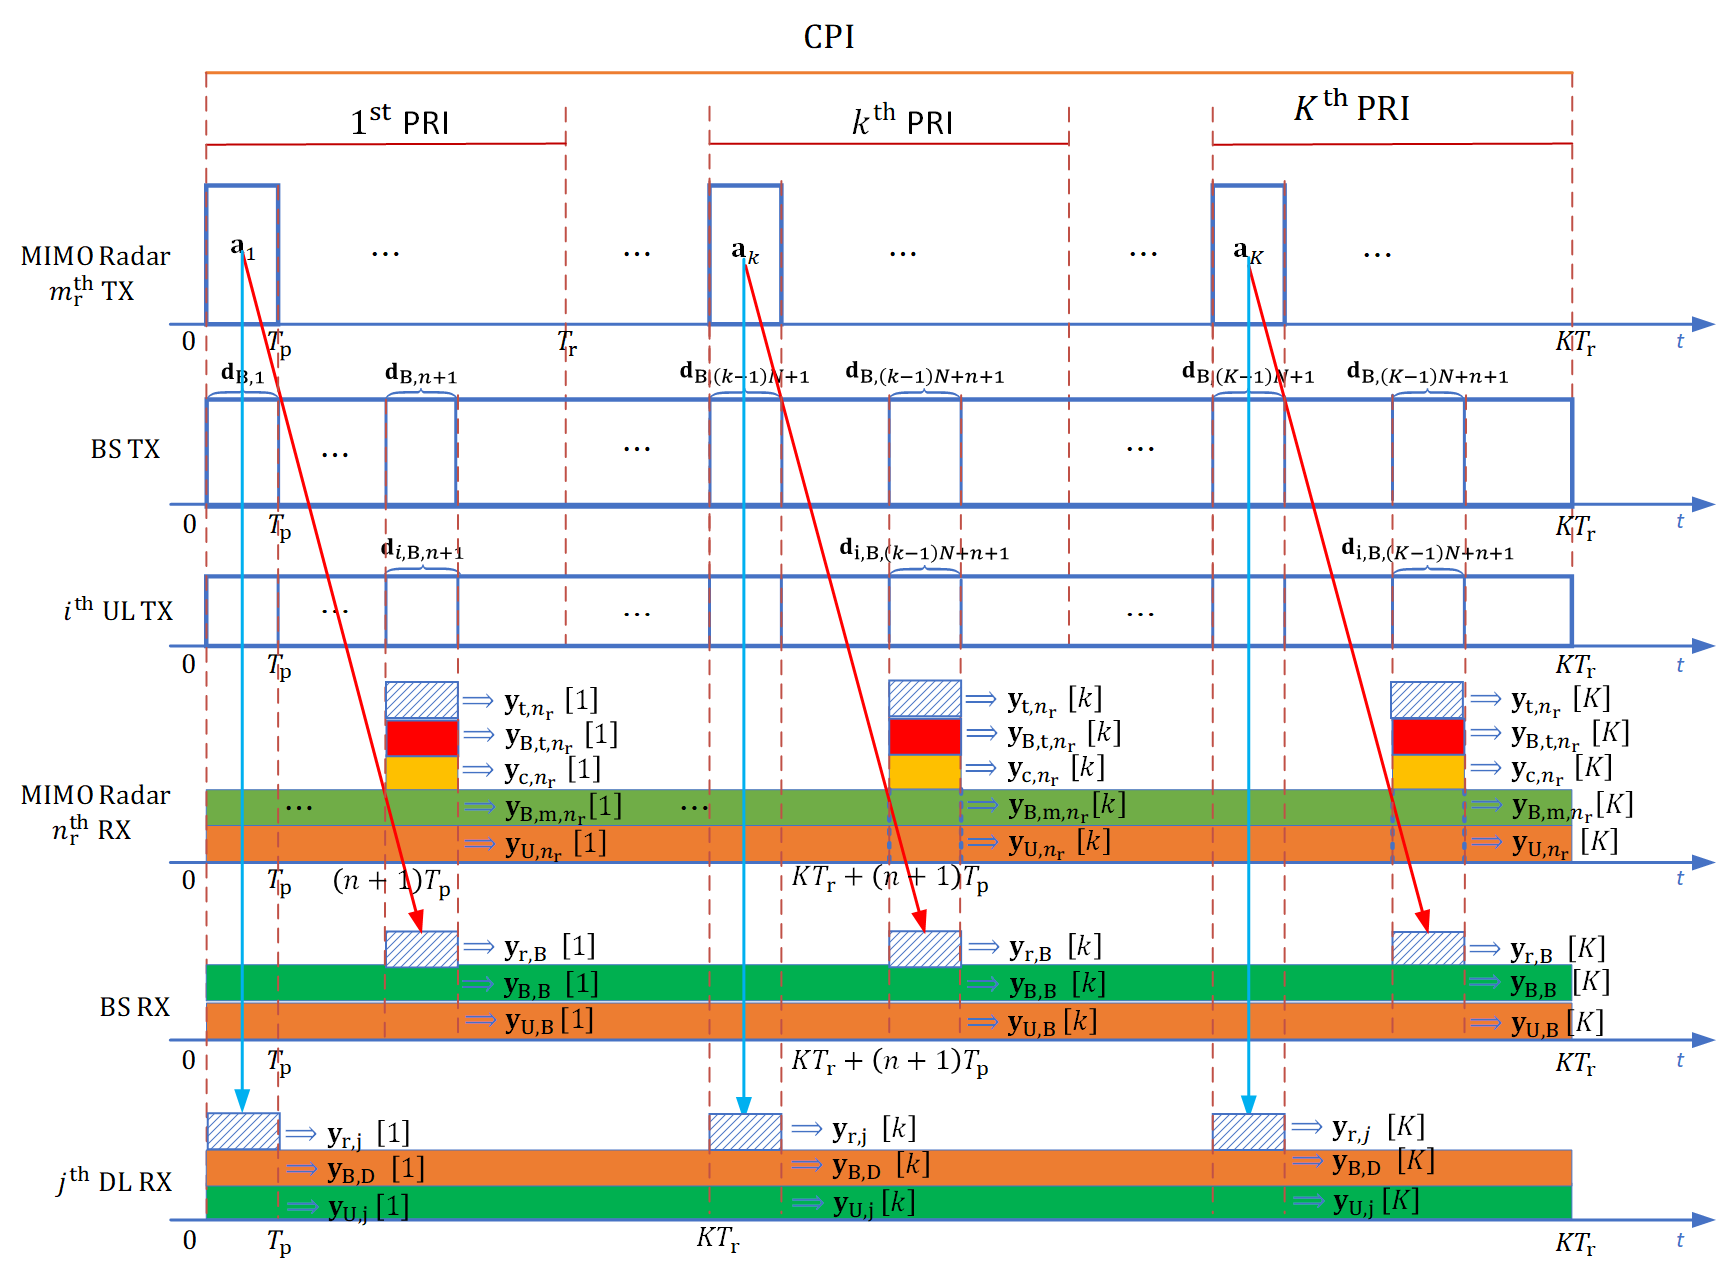
\includegraphics[width=3.1in]{Drawing3}
		%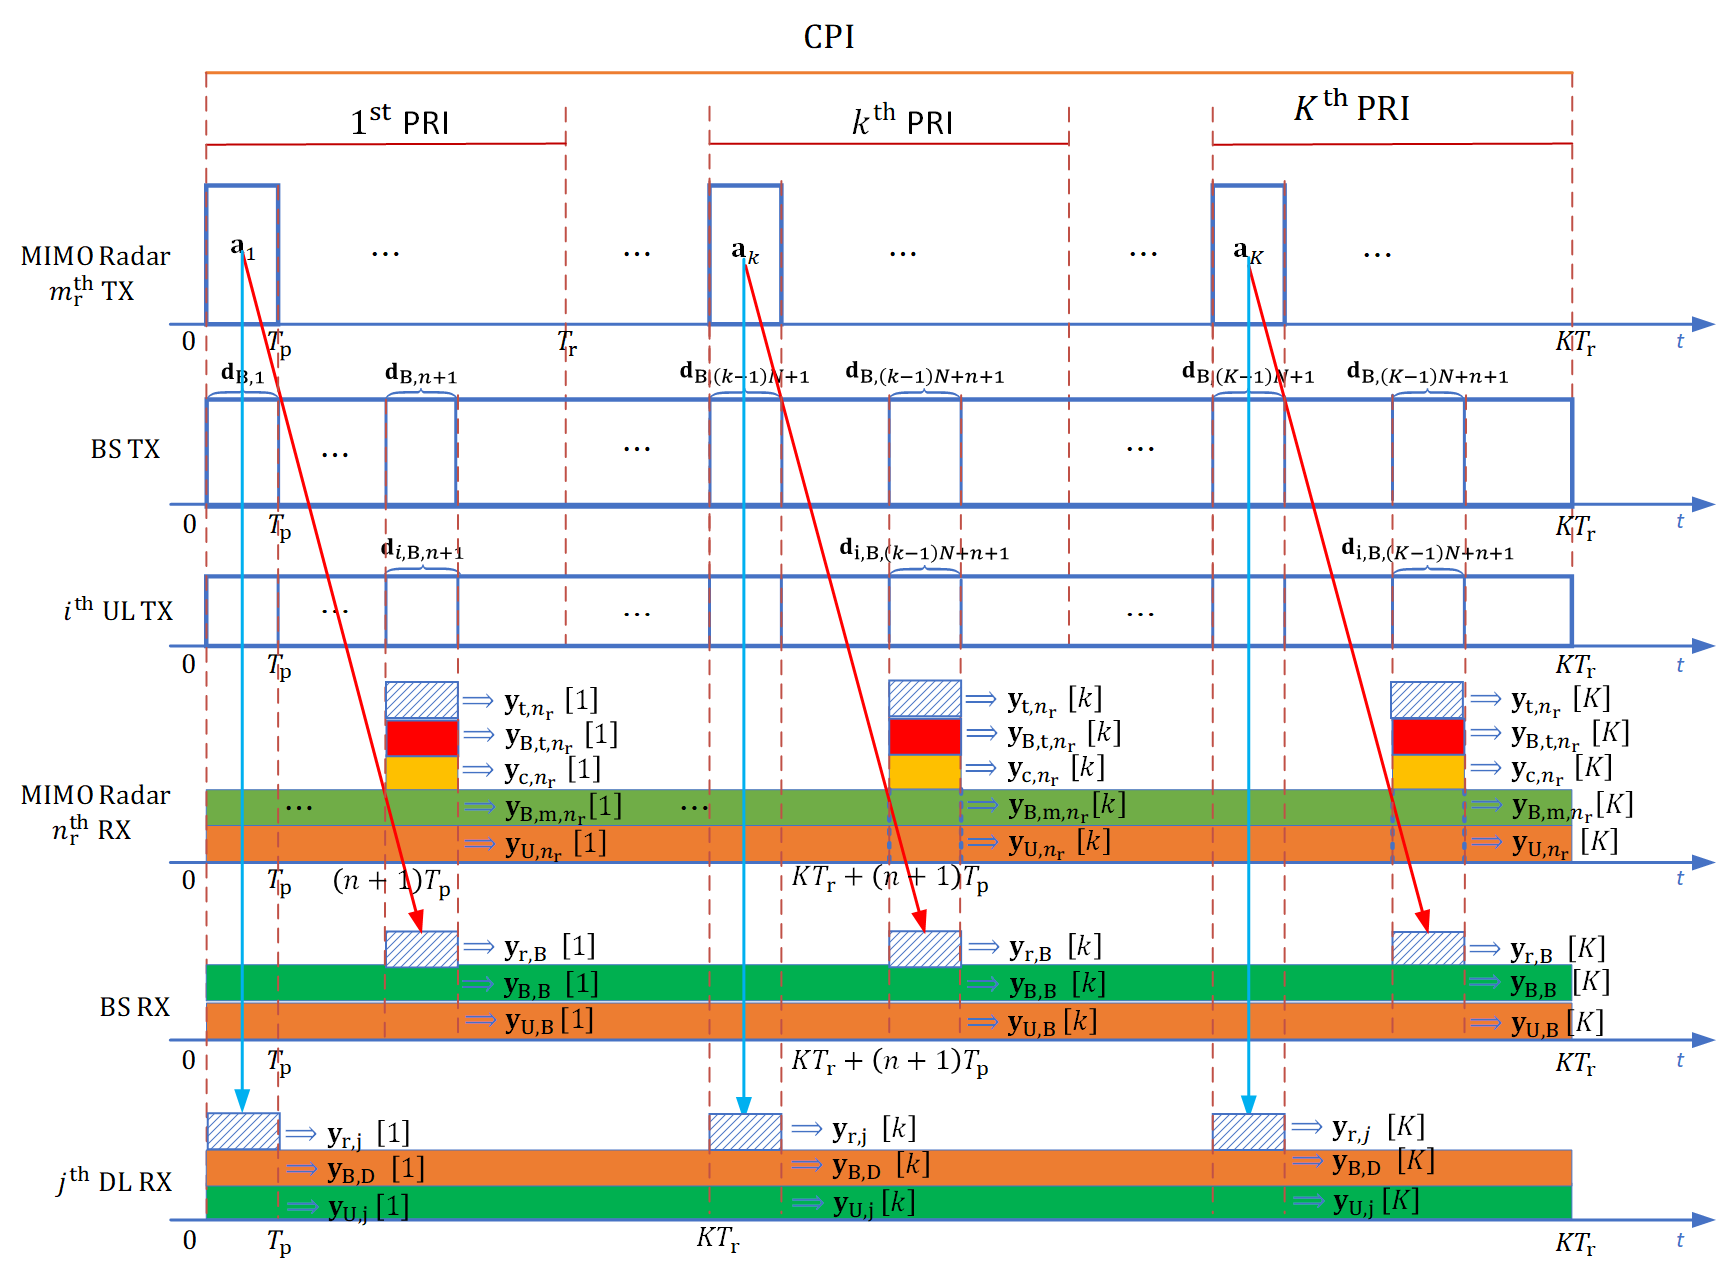
\includegraphics[width=0.80\textwidth]{Drawing3.png}
		%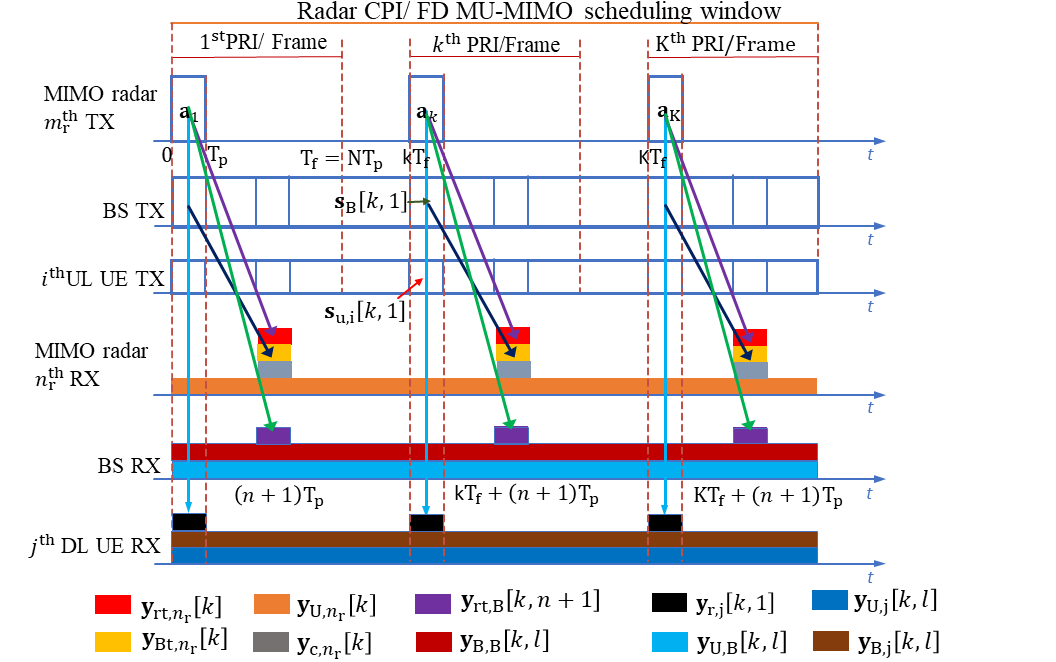
\includegraphics[width=0.80\textwidth]{systemmodel.png}
		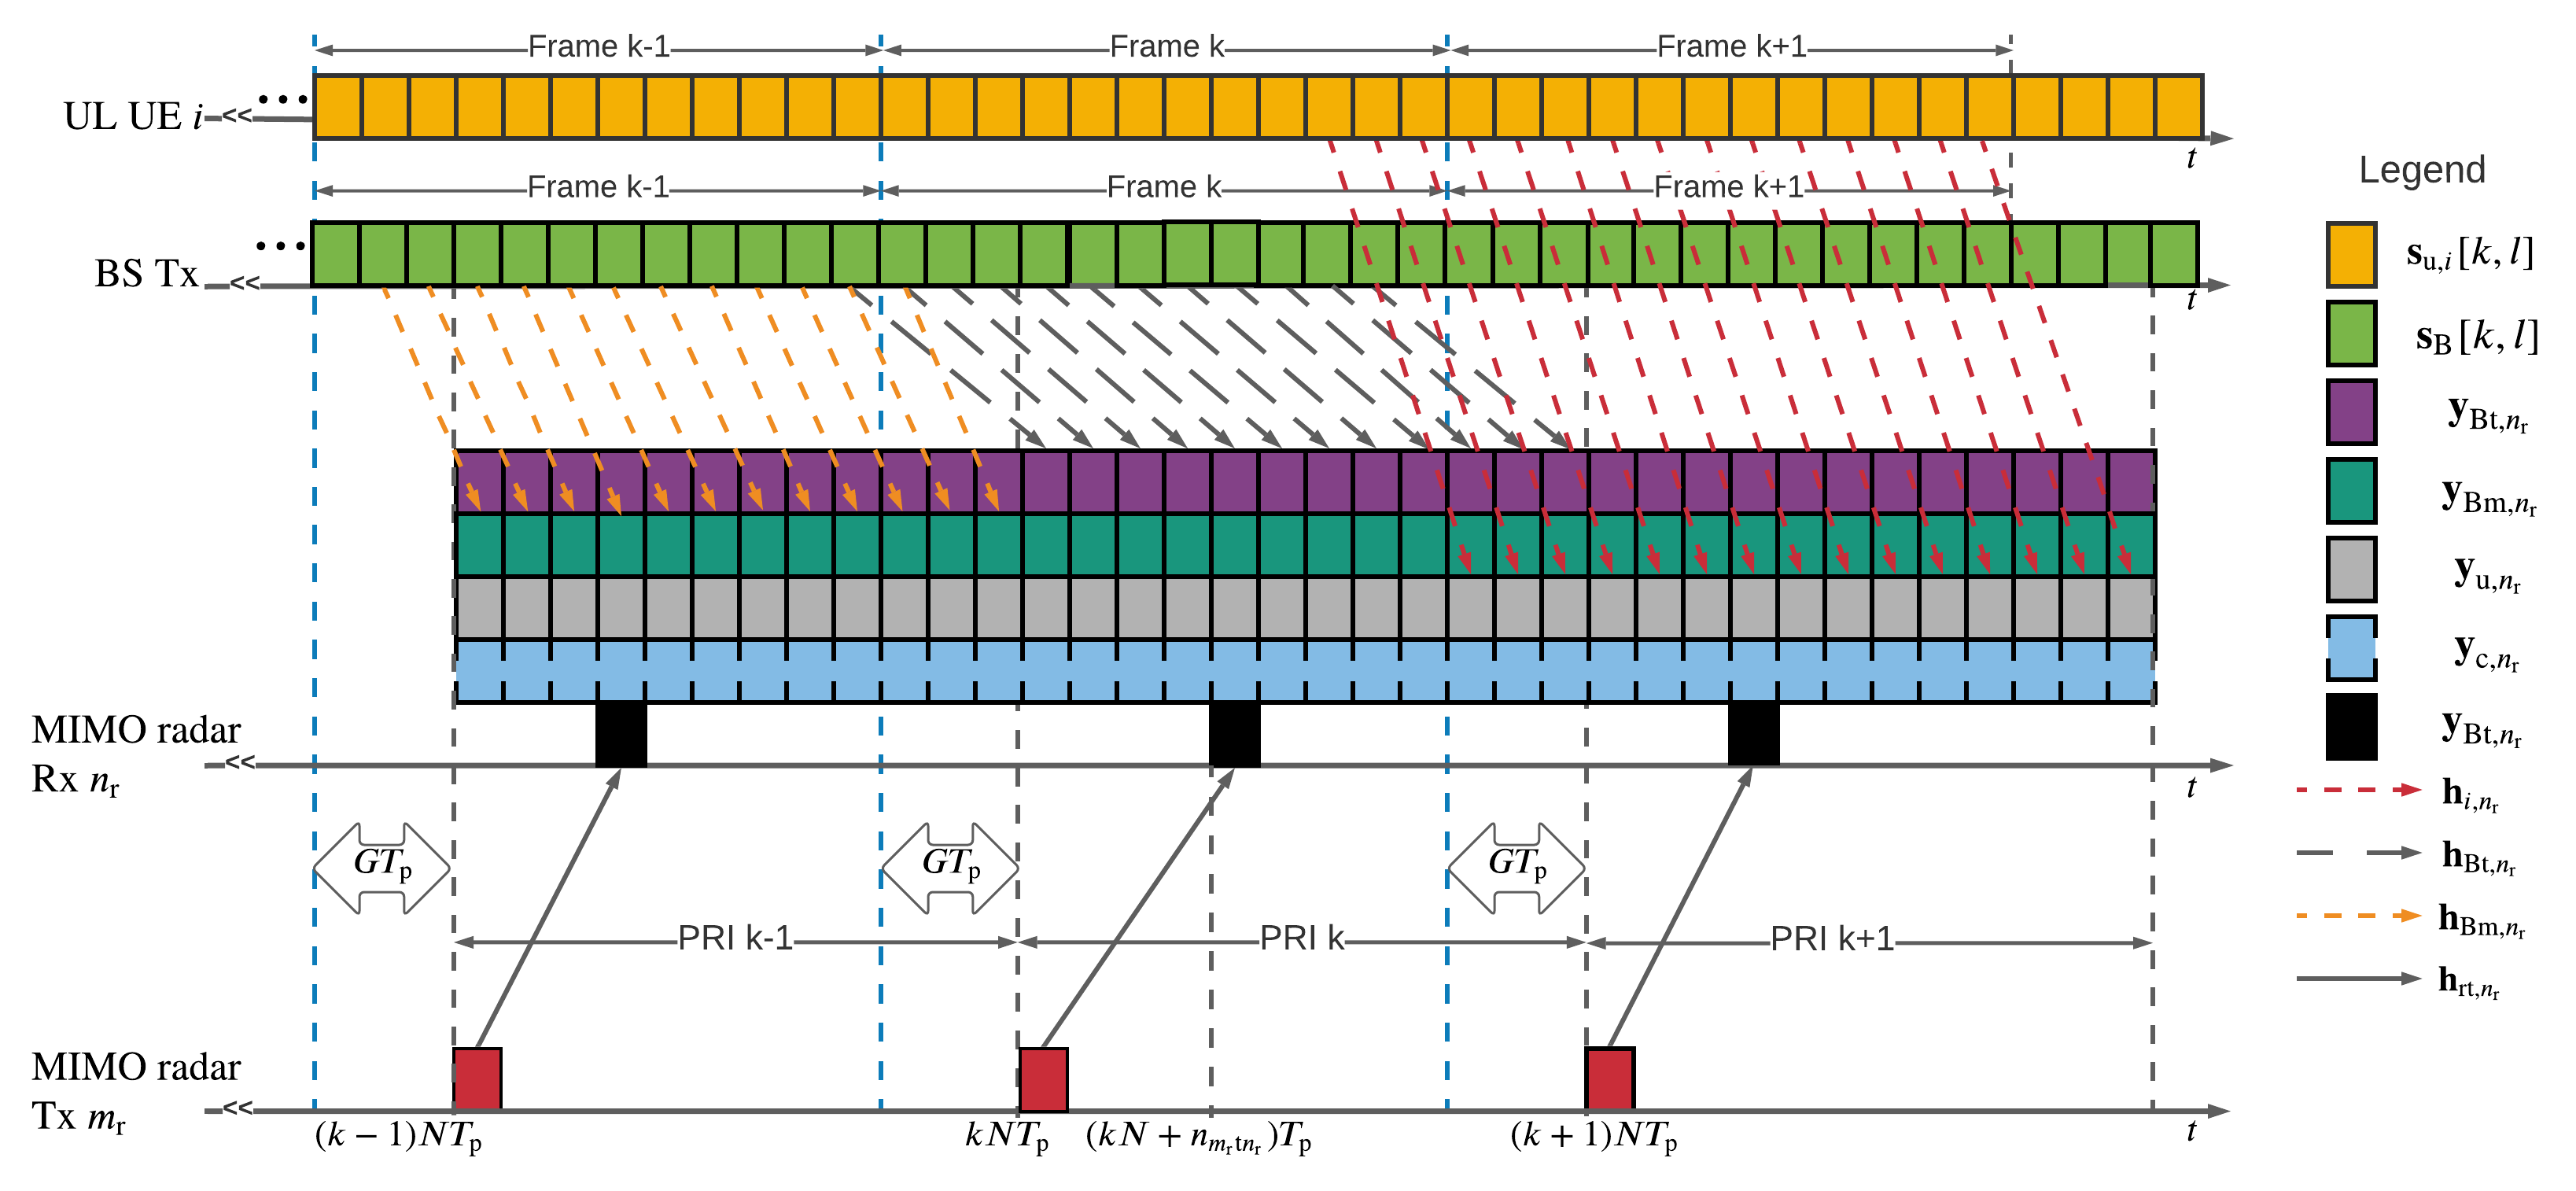
\includegraphics[width=1.0\columnwidth]{Timing_diagram_radar.png}
		\caption{\textcolor{red}{The overlaid signal timing diagram for the  signals observed at the radar Rx }
			%For each MIMO radar Rx, we focus on the $\ith{n}$ range cell where the target is observed. The $\ith{j}$ UE is interfered by the radar probing signal during the symbol period when the MIMO radar transmits pulses. %\textcolor{red}{\textbf{The top text is cut off.}}
		} 
		%\vspace{-2em}
		\label{fig:systemmodel}
	\end{figure}
	
	
	
	
	
	\color{black}
	\section{CWSM Maximization}
	\label{sec: formulation}
	%In this section, we derive the CWSM expression before formulating the CWSM maximization problem based on the proposed spectral co-design model in Section \ref{sec:system}. 
	The performance metrics to design radar and communications systems are not identical because of different system goals. For example, in general, a communications system strives to achieve high data rates while a radar performs detection, estimation, and tracking. Some recent works \cite{alaee2020information,dokhanchi2020multi,ni2020waveform} suggest MI as a common performance metric. The MI is a well-studied metric in MU-MIMO communications for transmit precoder design\cite{Luo2011IterativeWMMSE}. A number of works recently on radar code design adopt the MI as design criteria\cite{Colornoise_waveform,Jammer_game,NaghshTSP2017,JianLi2019,20MISTAP}. %Later, MI-based \textcolor{red}{radar code design} was also extended to MIMO radars \cite{Jammer_game,NaghshTSP2017}. 
	It has been shown \cite{Jammer_game} that maximizing the MI between the radar received signal and the target response leads to a better detection performance in the presence of the Gaussian noise. For our co-design, we propose a more effective common performance measure by combining the MI-based information theoretic perspective of radar waveform design with the conventional weighted sum rate maximization for MU-MIMO systems into a new CWSM metric.
	%In this work, the MI of the MIMO radar is defined as the MI between the output of the linear receiver and the channel target response. 
	
	%The co-design of the MIMO radar transceiver involves applying a linear receive filter bank at each MIMO radar Rx. Denote the receiver of the $\ith{n\rr}$ Rx by $\mathbf{U}_{\mathrm{r},n\rr}\in\mathbb{C}^{\mathit{M}\rr\times K}$ whose output  $\widetilde{\mathbf{y}}\rnr$ is\par\noindent\small
	
	%\begin{IEEEeqnarray}{rCl}
	%\widetilde{\mathbf{y}}\rnr&=&\mathbf{U}\rnr\mathbf{y}\rnr\nonumber\\
	%&=&\mathbf{U}\rnr\paren{\mathbf{S}_{\mathrm{rt},n\rr}\mathbf{h}_{\mathrm{rt},n\rr}+\mathbf{S}_{\mathrm{Bt},n\rr}\mathbf{h}_{\mathrm{Bt},n\rr}}+\widetilde{\mathbf{y}}^{\mathrm{in}}_{\mathrm{r},n\rr}
	%\end{IEEEeqnarray}\normalsize
	%where $\widetilde{\mathbf{y}}^{\mathrm{in}}_{\mathrm{r},n\rr}=\mathbf{U}\rnr\mathbf{y}_{\mathrm{in},n\rr}$. %\textcolor{red}{matrices $\mathbf{U}$ have never been defined earlier?}. 
	%As we assume that both
	%As $\mathbf{h}_{\mathrm{rt},n\rr}$ and $\mathbf{h}_{\mathrm{Bt},n\rr}$ contain target information, the conditional MI between $\widetilde{\mathbf{y}}\rnr$ and jointly $\mathbf{h}_{\mathrm{rt},n\rr}$ and $\mathbf{h}_{\mathrm{Bt},n\rr}$ given the radar transmit codes $\mathbf{A}$ can be written as\par\noindent\small
	%\begin{IEEEeqnarray}{rCl}
	%\mathit{I}\rnr&\triangleq&\mathit{I}\paren{\widetilde{\mathbf{y}}\rnr;\mathbf{h}_{\mathrm{rt},n\rr},\mathbf{h}_{\mathrm{Bt},n\rr}|\mathbf{A}}\nonumber\\
	%&=&I\paren{\widetilde{\mathbf{y}}\rnr;\mathbf{h}_{\mathrm{rt},n\rr}|\mathbf{A}}+I\paren{\widetilde{\mathbf{y}}\rnr;\mathbf{h}_{\mathrm{Bt},n\rr}|\mathbf{h}_{\mathrm{rt},n\rr},\mathbf{A}}\nonumber%\\
	%&=&\mathit{H}\paren{\widetilde{\mathbf{y}}\rnr|\mathbf{A}}-\mathit{H}\paren{\widetilde{\mathbf{y}}\rnr|\mathbf{h}_{\mathrm{rt},n\rr},\mathbf{h}_{\mathrm{Bt},n\rr},\mathbf{A}}\nonumber\\
	%&=&\mathit{H}\paren{\widetilde{\mathbf{y}}\rnr|\mathbf{A}}-\mathit{H}\paren{\widetilde{\mathbf{y}}^{\mathrm{in}}_{\mathrm{r},n\rr}|\mathbf{A}}
	%\end{IEEEeqnarray}\normalsize
	%where $\mathit{H}\paren{\widetilde{\mathbf{y}}\rnr|\mathbf{A}}$ and  $\mathit{H}\paren{\widetilde{\mathbf{y}}^{\mathrm{in}}_{\mathrm{r},n\rr}|\mathbf{A}}$ denote the conditional differential entropies of $\widetilde{\mathbf{y}}\rnr$ given $\mathbf{A}$ and $\widetilde{\mathbf{y}}^{\mathrm{in}}_{\mathrm{r},n\rr}$, respectively, and the last equality is because after observing $\mathbf{h}_{\mathrm{rt},n\rr}$ and $\mathbf{h}_{\mathrm{Bt},n\rr}$, the only uncertainty remaining in $\widetilde{\mathbf{y}}\rnr$ is due to $\widetilde{\mathbf{y}}_{\text{in},n\rr}$, and since $\mathbf{y}_{\text{in},n\rr}$ and $\mathbf{h}_{\mathrm{rt},n\rr}$ as well as $\mathbf{h}_{\mathrm{Bt},n\rr}$ are independent, the last equality holds. By the definition of the conditional differential entropy with the Gaussian noise, one can obtain that \cite{cover2006elements}\par\noindent\small
	%\begin{IEEEeqnarray}{rCl}
	%\mathit{H}\paren{\widetilde{\mathbf{y}}\rnr|\mathbf{A}}&=&\rho+\log\left|\mathbf{U}\rnr\mathbf{R}_{\mathrm{r},n\rr}\mathbf{U}^\dagger\rnr \right|\\
	%\mathit{H}\paren{\widetilde{\mathbf{y}}^{\mathrm{in}}_{\mathrm{r},n\rr}|\mathbf{A}}&=&\rho+\log\left|\mathbf{U}\rnr\mathbf{R}^{\mathrm{in}}_{\mathrm{r},n\rr}\mathbf{U}^\dagger\rnr \right|
	%\end{IEEEeqnarray}\normalsize
	%where the constant $\rho=K\log\paren{\pi}+K$. This leads to\par\noindent\small
	%\begin{IEEEeqnarray}{rCl}\label{radarmi}
	%\mathit{I}\rnr&=&\log\frac{\left|\mathbf{U}\rnr\paren{\mathbf{R}_{\mathrm{rt},n\rr}+\mathbf{R}_{\mathrm{Bt},n\rr}+\mathbf{R}^{\mathrm{in}}_{\mathrm{r},n\rr}}\mathbf{U}^\dagger\rnr \right|}{\left|\mathbf{U}\rnr\mathbf{R}^{\mathrm{in}}_{\mathrm{r},n\rr}\mathbf{U}^\dagger\rnr \right|}\nonumber\\
	%&=&\log\left|
	%\sizecorr{\paren{\mathbf{U}\rnr\mathbf{R}^{\mathrm{in}}_{\mathrm{r},n\rr}\mathbf{U}^\dagger\rnr}^{-1}}
	%\mathbf{I}+\mathbf{U}\rnr\paren{\mathbf{R}_{\mathrm{rt},n\rr}+\mathbf{R}_{\mathrm{Bt},n\rr}}\mathbf{U}^\dagger\rnr\right.\nonumber\\
	%&&\left.\paren{\mathbf{U}\rnr\mathbf{R}^{\mathrm{in}}_{\mathrm{r},n\rr}\mathbf{U}^\dagger\rnr}^{-1}\right|
	%\end{IEEEeqnarray}\normalsize
	%With $\mathbf{h}_{\mathrm{rtr}}\triangleq\vect\braces{\mathbf{H}_{\mathrm{rtr}}}$ and $\mathbf{h}_{\mathrm{Btr}}\triangleq\vect\braces{\mathbf{H}_{\mathrm{Btr}}}$, the resulting MI between $\widetilde{\mathbf{y}}\rr=\sum_{n\rr=1}^{\mathit{N}\rr}\widetilde{\mathbf{y}}\rnr$ and, jointly $\mathbf{h}_{\mathrm{rtr}}$ and $\mathbf{h}_{\mathrm{Btr}}$ is \par\noindent\small
	%\begin{IEEEeqnarray}{rCl}
	%I\rr&\triangleq&\mathit{I}\paren{\mathbf{y}\rr;\mathbf{h}_{\mathrm{rtr}},\mathbf{h}_{\mathrm{Btr}}|\mathbf{A}}=\sum_{n\rr=1}^{\mathit{N}\rr}\mathit{I}\rnr
	%\end{IEEEeqnarray}\normalsize
	%\begin{IEEEeqnarray}{rCl}\label{radarmi}
	%\mathit{I}\paren{\mathbf{y}\rr;\mathbf{h}_{\mathrm{rt},n\rr},\mathbf{h}_{\mathrm{Bt},n\rr}|\mathbf{A}}&=&\log\frac{\left|\mathbf{R}_{\mathrm{rt},n\rr}+\mathbf{R}_{\mathrm{Bt},n\rr}+\mathbf{R}^{\mathrm{in}}_{\mathrm{r},n\rr} \right|}{\left|\mathbf{R}^{\mathrm{in}}_{\mathrm{r},n\rr} \right|}\nonumber\\
	%&=&\log\left|\mathbf{I}_{KN\rr}+\mathbf{R}^{-1}_{\mathrm{in,r}}\paren{\mathbf{R}_{\mathrm{rt},n\rr}+\mathbf{R}_{\mathrm{Bt},n\rr}}\right|. \IEEEeqnarraynumspace
	%\end{IEEEeqnarray}
	%and we define $\mathbf{W}^{\mathrm{MMSE}}_{\textrm{B},k}\triangleq\mathbf{W}^{\mathrm{MMSE}}_{\textrm{B},\paren{k-1}N+n+1}$ to lighten the notation. 
	To derive CWSM, 
	$\stnrk=\mathbf{J}_{\textrm{r}}\mathbf{a}\bracket{k}+\mathbf{J}_{\mathrm{B}}\sBtnrk$, where $\mathbf{J}_{\textrm{r}}=\bracket{\mathbf{I}_{\mathit{M}\rr\times \mathit{M}\rr};\mathbf{0}_{\mathit{M}\cc\times \mathit{M}\rr}}\in\mathbb{R}^{\mathbf{\mathit{M}\times \mathit{M}\rr}}$ and $\mathbf{J}_{\mathrm{B}}=\bracket{\mathbf{0}_{\mathit{M}\rr\times \mathit{M}\cc};\mathbf{I}_{\mathit{M}\cc\times \mathit{M}\cc}}\in\mathbb{R}^{\mathbf{\mathit{M}\times \mathit{M}\cc}}$
	let the LRF at the $\ith{n\rr}$ MIMO radar Rx be $\mathbf{U}_{\mathrm{r},n\rr}=\bracket{\mathbf{u}_{\mathrm{r},n\rr}\bracket{1},\cdots,\mathbf{u}_{\mathrm{r},n\rr}\bracket{\mathit{K}}}\in\mathbb{C}^{KM\times\mathrm{\mathit{K}}}$, which is applied to $\mathbf{y}_{\mathrm{r},n\rr}$ as
	\par\noindent\small
	\begin{IEEEeqnarray}{rCl}
		\widetilde{\mathbf{y}}_{\textrm{r},n\rr}&=&\underbrace{\sum_{k=1}^{\mathit{K}}\urk y_{\mathrm{t},n\rr}\bracket{k}}_{\widetilde{\mathbf{y}}_{\mathrm{t},n\rr}}+\underbrace{\sum_{k=1}^{\mathit{K}}\urk y^{\mathrm{in}}_{\mathrm{r},n\rr}\bracket{k}}_{\widetilde{\mathbf{y}}^{\mathrm{in}}_{\mathrm{r},n\rr}}
		%	\widetilde{\mathbf{y}}_{\textrm{r},n\rr}&=&\mathbf{U}\rnr\paren{\mathbf{s}_{\textrm{rt},n\rr}\mathbf{h}_{\mathrm{rt},n\rr}+\mathbf{s}_{\textrm{Bt},n\rr}\mathbf{h}_{\mathrm{Bt},n\rr}}+\mathbf{U}\rnr\mathbf{y}_{\textrm{in},n\rr}\nonumber\\
	\end{IEEEeqnarray}\normalsize
	%Define $\mathbf{S}_{\target,n\rr}=\bracket{\mathbf{s}_{\textrm{t},n\rr}\bracket{1},\cdots,\mathbf{s}_{\textrm{t},n\rr}\bracket{\mathrm{\mathit{K}}}}$
	Since $\mathbf{h}_{\mathrm{t},n\rr}$ contains the target information, the MI between $\widetilde{\mathbf{y}}_{\mathrm{r},n\rr}$ %\textcolor{red}{what is this?} 
	and 
	%jointly $\mathbf{h}_{\mathrm{rt},n\rr}$ and
	$\mathbf{h}_{\mathrm{t},n\rr}$ conditioned on the radar code matrix $\mathbf{A}$ is derived using the chain rule as \cite{Colornoise_waveform,Jammer_game}\par\noindent\small
	\begin{IEEEeqnarray}{rCl}
		\mathit{I}\rnr&\triangleq&\mathit{I}\paren{\widetilde{\mathbf{y}}\rnr;\mathbf{h}_{\mathrm{t},n\rr}|\mathbf{A}}=\mathit{H}\paren{\widetilde{\mathbf{y}}\rnr|\mathbf{A}}-\mathit{H}\paren{\widetilde{\mathbf{y}}\rnr|\mathbf{h}_{\mathrm{t},n\rr},\mathbf{A}}\nonumber\\
		%&=&I\paren{\widetilde{\mathbf{y}}\rnr;\mathbf{h}_{\mathrm{rt},n\rr}|\mathbf{A}}+I\paren{\widetilde{\mathbf{y}}\rnr;\mathbf{h}_{\mathrm{Bt},n\rr}|\mathbf{h}_{\mathrm{rt},n\rr},\mathbf{A}}\nonumber\\
		%&=&\mathit{H}\paren{\widetilde{\mathbf{y}}\rnr|\mathbf{A}}-\mathit{H}\paren{\widetilde{\mathbf{y}}\rnr|\mathbf{h}_{\mathrm{t},n\rr},\mathbf{A}}\nonumber\\
		&=&\mathit{H}\paren{\widetilde{\mathbf{y}}\rnr|\mathbf{A}}-\mathit{H}\paren{\widetilde{\mathbf{y}}_{\textrm{t},n\rr}|\mathbf{h}_{\mathrm{t},n\rr},\mathbf{A}}-\mathit{H}\paren{\widetilde{\mathbf{y}}^{\mathrm{in}}_{\mathrm{r},n\rr}|\mathbf{h}_{\mathrm{t},n\rr},\mathbf{A}}\nonumber\\
		&=&\mathit{H}\paren{\widetilde{\mathbf{y}}\rnr|\mathbf{A}}-\mathit{H}\paren{\widetilde{\mathbf{y}}^{\mathrm{in}}_{\mathrm{r},n\rr}|\mathbf{A}},
	\end{IEEEeqnarray}\normalsize
	where the last equality holds because $\widetilde{\mathbf{y}}^{\mathrm{in}}_{\mathrm{r},n\rr}$ entirely depends on $\mathbf{A}$ such that $\mathit{H}\paren{\widetilde{\mathbf{y}}_{\textrm{t},n\rr}|\mathbf{h}_{\mathrm{t},n\rr}}$  and $\mathbf{h}_{\mathrm{t},n\rr}$ as well as  $\widetilde{\mathbf{y}}^{\mathrm{in}}_{\mathrm{r},n\rr}$ and $\mathbf{h}_{\mathrm{t},n\rr}$ are mutually independent. By the definition of the conditional differential entropy with the Gaussian noise \cite{Colornoise_waveform},  \par\noindent\small
	\begin{IEEEeqnarray}{rCl}
		\mathit{H}\paren{\widetilde{\mathbf{y}}\rnr|\mathbf{A}}&=&\varrho+\log\left|\mathbf{U}\rnr\mathbf{R}_{\mathrm{r},n\rr}\mathbf{U}^\dagger\rnr \right|,\nonumber\\
		\mathit{H}\paren{\widetilde{\mathbf{y}}^{\mathrm{in}}_{\mathrm{r},n\rr}|\mathbf{A}}&=&\varrho+\log\left|\mathbf{U}\rnr\mathbf{R}^{\mathrm{in}}_{\mathrm{r},n\rr}\mathbf{U}^\dagger\rnr \right|,\nonumber
	\end{IEEEeqnarray}\normalsize
	where the constant $\varrho=K\log\paren{\pi}+K$. This leads to\par\noindent\small
	\begin{IEEEeqnarray}{rCl}\label{radarmi}
		\mathit{I}\rnr&=&\log\frac{\left|\mathbf{U}\rnr\paren{\mathbf{R}_{\mathrm{t},n\rr}+\mathbf{R}^{\mathrm{in}}_{\mathrm{r},n\rr}}\mathbf{U}^\dagger\rnr \right|}{\left|\mathbf{U}\rnr\mathbf{R}^{\mathrm{in}}_{\mathrm{r},n\rr}\mathbf{U}^\dagger\rnr \right|}\nonumber\\
		&=&\log\left\lvert\mathbf{I}+\mathbf{U}\rnr\mathbf{R}_{\textrm{t},n\rr}\mathbf{U}^\dagger\rnr\paren{\mathbf{U}\rnr\mathbf{R}^{\mathrm{in}}_{\mathrm{r},n\rr}\mathbf{U}^\dagger\rnr}^{-1}\right\rvert.
		%&=&\log\left|
		% \sizecorr{\paren{\mathbf{U}\rnr\mathbf{R}^{\mathrm{in}}_{\mathrm{r},n\rr}\mathbf{U}^\dagger\rnr}^{-1}}
		%\mathbf{I}+\mathbf{U}\rnr\mathbf{R}_{\textrm{t},n\rr}\mathbf{U}^\dagger\rnr\right.\nonumber\\
		%&&\left.\paren{\mathbf{U}\rnr\mathbf{R}^{\mathrm{in}}_{\mathrm{r},n\rr}\mathbf{U}^\dagger\rnr}^{-1}\right|. 
	\end{IEEEeqnarray}\normalsize
	\iffalse
	With $\mathbf{h}_{\mathrm{rtr}}\triangleq\vect\braces{\mathbf{H}_{\mathrm{rtr}}}$ and $\mathbf{h}_{\mathrm{Btr}}\triangleq\vect\braces{\mathbf{H}_{\mathrm{Btr}}}$, the resulting MI between $\widetilde{\mathbf{y}}\rr=\sum_{n\rr=1}^{\mathit{N}\rr}\widetilde{\mathbf{y}}\rnr$ and, jointly $\mathbf{h}_{\mathrm{rtr}}$ and $\mathbf{h}_{\mathrm{Btr}}$ is \par\noindent\small
	\begin{IEEEeqnarray}{rCl}
		I\rr&\triangleq&\mathit{I}\paren{\mathbf{y}\rr;\mathbf{h}_{\mathrm{rtr}},\mathbf{h}_{\mathrm{Btr}}|\mathbf{A}}=\sum_{n\rr=1}^{\mathit{N}\rr}\mathit{I}\rnr
	\end{IEEEeqnarray}\normalsize	
	\fi
	
	The LRFs deployed at the BS to decode the $\ith{i}$ UL UE and the $\ith{j}$ DL UE during the $\ith{k}$ frame of the observation window are denoted by $\UiB\in\mathbb{C}^{\mathit{D}_{\mathrm{u},i}\times \mathit{N}\cc}$ and $\UBj\in\mathbb{C}^{\mathit{D}_{\mathrm{d},j}\times \mathit{N}_{\mathrm{d},j}}$, respectively. With the outputs of $\UiB$ and $\UBj$ being $\widetilde{\mathbf{y}}_{\mathrm{u},i}\bracket{k,l}$ and $\widetilde{\mathbf{y}}_{\mathrm{d},j}\bracket{k,l}$, respectively, the MIs between $\widetilde{\mathbf{y}}_{\mathrm{u},i}\bracket{k,l}$ and $\mathbf{s}_{\mathrm{u},i}\bracket{k,l}$ as well as $\widetilde{\mathbf{y}}_{\mathrm{d},j}\bracket{k,l}$ and $\mathbf{s}_{\mathrm{d},j}\bracket{k,l}$ are shown as \par\noindent\small
	\begin{flalign}
		&\mathit{I}_{\mathrm{u},i}\bracket{k,l}\triangleq \mathit{I}\paren{\mathbf{s}_{\mathrm{u},i}\bracket{k,l};\widetilde{\mathbf{y}}_{\mathrm{u},i}\bracket{k,l}|\mathbf{H}_{i,\B}}=\\
		&\log\left|\mathbf{I}_{D_{\mathrm{u},i}}+\UiB\mathbf{R}_{\mathrm{u},i}\bracket{k,l}\UiBH\paren{\UiB\mathbf{R}^{\mathrm{in}}_{\mathrm{u},i}\bracket{k,l}\UiBH}^{-1}\right|\nonumber
	\end{flalign}\normalsize
	\par\noindent\small
	\begin{flalign}
		&\text{and }\mathit{I}_{\mathrm{d},j}\bracket{k,l}\triangleq I\paren{\mathbf{s}_{\mathrm{B},j}\bracket{k,l};\widetilde{\mathbf{y}}_{\mathrm{d},j}\bracket{k,l}|\mathbf{H}_{\B,j}}=\label{DLmutual}\\
		&\log\left|\mathbf{I}_{D_{\mathrm{d},j}}+\UBj\mathbf{R}_{\mathrm{d},j}\bracket{k,l}\UBjH\paren{\UBj\mathbf{R}^{\mathrm{in}}_{\mathrm{d},j}\bracket{k,l}\UBjH}^{-1}\right|\nonumber
	\end{flalign}\normalsize
	%Recall from section \ref{Coexistence} that the worst interference scenarios occur to the BS and the DL UEs during the $\ith{\paren{n+1}}$ and $1^{\textrm{st}}$ symbol periods of each frame, respectively, i.e., $I_{i,\B}\paren{k,\ell}\geq I_{i,\B}\bracket{k}$ and $I_{\B,j}\bracket{m,l}\geq I_{\B,j}\bracket{k}$. 
	%The performance metric CWSM is the weighted sum of the MIs of the signal received at \textcolor{red}{is this right? what is meant by signal rxed at the comm link?} all radar Rx and communications links, namely,
	respectively. Recall that we evaluate the FD communications system based on the $\ith{n_{\mathrm{rtB}}}$ and $\ith{n_{{rmB}}}$ symbol periods of each UL frame and the $\ith{n_{\mathrm{r,d}}}$ symbol period of each DL frame within the observation, which implies the worst case interference scenario from the MIMO radar. The performance metric CWSM is thus defined as the weighted sum of the communications' MIs  related to the aforementioned symbol periods as well as $I_{\mathrm{r},n\rr}$ for all $n\rr$,   %In the sequel, for notational simplicity, we omit the symbol period index for notational simplicity. 
	\par\noindent\small
	\begin{flalign}
		\label{objectfunction1}
		\mathit{I}_{\textrm{CWSM}}=&\sum_{n\rr=1}^{\mathit{N}\rr}\alpha^\textrm{r}_{n\rr} \mathit{I}_{\textrm{r},n\rr}+\sum_{k=1}^\mathit{K}\sum_{i=1}^\mathit{I}\alpha^\textrm{u}_i\paren{\mathit{I}_{\mathrm{u},i}\bracket{k,n_{\mathrm{rtB}}}+\mathit{I}_{\mathrm{u},i}\bracket{k,n_{\mathrm{rmB}}}}\nonumber\\
		&+\sum_{k=1}^\mathit{K}\sum_{j=1}^\mathit{J}\alpha^\textrm{d}_j\mathit{I}_{\mathrm{d},j}\bracket{k,n_{\mathrm{r,d}}},
	\end{flalign}
	%\end{IEEEeqnarray}
	\normalsize
	where $\alpha^\textrm{r}_{n\rr}$, $\alpha^\textrm{u}_i$, and $\alpha^\textrm{d}_j$ are pre-defined weights given to the MIMO radar Rx $n\rr$, $\ith{i}$ UL UE and $\ith{j}$ DL UE, respectively, for all $n\rr$, $i$, and $j$, which are \textcolor{red}{are determined by the system priority dependent on specific applications. For example, within the FD communications system, the weights can be chosen based on the available buffer capacities of the BS and UEs\cite{WMMSEWSR,FD_WMMSE,Lui2006subg}. For the joint radar communications system, one can assign higher weights to $\alpha^{\mathrm{r}}_{n_\mathrm{r}}$ when there are targets in the scene and lower ones when no targets are around, which leads to flexibility to achieve desired overall system performance\cite{Liu2018Gloabalsip}}.
	
	Define the sets of the UL and DL precoders as well as the set of LRFs as $\braces{\mathbf{P}}\triangleq\braces{\PiB,\PBj | i\in\mathbb{Z}_+\braces{I}, j\in\mathbb{Z}_+\braces{J}, k\in\mathbb{Z}_+\braces{K}}$
	\iffalse
	\par\noindent\small
	\begin{flalign}
		\braces{\mathbf{P}}\triangleq\braces{\PiB,\PBj | i\in\mathbb{Z}_+\braces{I}, j\in\mathbb{Z}_+\braces{J}, k\in\mathbb{Z}_+\braces{K}}\nonumber
	\end{flalign}\normalsize
	\fi
	%$\braces{\mathbf{ P}}\triangleq\braces{\PiB,\PBj,\forall i,j,k}$  and $\braces{\mathbf{ U}}\triangleq\braces{\UiB, \UBj, \mathbf{U}\rnr, \forall i,j,k,n\rr}$, 
	%$\braces{\mathbf{ P}}\triangleq\braces{\PiB,\PBj | 1 \le i \le I, 1\le j \le J, 1\le k \le K}$  
	and
	%$\braces{\mathbf{ U}}\triangleq\braces{\UiB, \UBj, \mathbf{U}\rnr | 1\le i \le I, 1\le j \le J, 1 \le k \le K, 1 \le n\rr \le N\rr}$.
	$\braces{\mathbf{U}}\triangleq\left\lbrace\UiB, \UBj, \mathbf{U}\rnr | i\in\mathbb{Z}_+\braces{I}, j\in\mathbb{Z}_+\braces{J},\right.$ $\left.k\in\mathbb{Z}_+\braces{K}, n\rr\in \mathbb{Z}_+\braces{N\rr}\right\rbrace$. 
	%Denote the maximum transmission powers dictated by the DL and UL link budgets as $\mathit{P}_\B$ and $\mathit{P}_{\textrm{U}}$, respectively. 
	The transmission powers occurred to the BS and the UL UE $i$ at the $\ith{k}$ frame are $P_{\mathrm{d}}\bracket{k}=\sum_{j=1}^{J}\mathit{P}_{\mathrm{d},j}\bracket{k}=\sum_{j=1}^{J}\trace\braces{\PBj\PBjH}$ and $\mathit{P}_{\mathrm{u},i}\bracket{k}$ $=\trace\braces{\PiB\PiBH}$, respectively, which are upper bounded by the maximum DL and UL powers $\mathit{P}_\B$ and $\mathit{P}_{\mathrm{U}}$, respectively. Denote the achievable rates for the UL UE $i$ and the DL UE $j$ in the $\ith{l}$ symbol period $\ith{k}$ frame by $R_{\mathrm{u},i}\bracket{k,l}$ and $R_{\mathrm{d},j}\bracket{k,l}$ and IBFD MU-MIMO QoS is quantified by the least acceptable achievable rates for the UL and DL denoted as $\mathit{R}_{\mathrm{UL}}$ and $\mathit{R}_{\mathrm{DL}}$, respectively. Next, we jointly design precoders $\braces{\mathbf{P}}$, radar code matrix $\mathbf{A}$, and LRFs $\braces{\mathbf{U}}$ by maximizing CWSM as \par\noindent\small
	\begin{IEEEeqnarray}{rCl}\label{jointop}
		\IEEEyesnumber\IEEEyessubnumber*
		%\braces{\mathbf{P}_{i,\textrm{B}}}_{i=1}^I,\braces{\mathbf{P}_{\textrm{B},j}}_{j=1}^J,\\ \mathbf{A},\mathbf{d}_{\B,j}
		&\underset{{\braces{\mathbf{P}},\braces{\mathbf{U}},
				\mathbf{A}}}{\text{maximize}}\;& \mathit{I}_{\textrm{CWSM}}\paren{\braces{\mathbf{U}},\braces{\mathbf{P}},\mathbf{A}}   \IEEEeqnarraynumspace\\
		&\text{subject to}\;& P_{\mathrm{d}}\bracket{k}\leq \mathit{P}_\textrm{B}, \label{DL_power}\\*
		&&\mathit{P}_{\mathrm{u},i}\bracket{k}\leq \mathit{P}_\textrm{U}, \label{UL_power}\\*
		&&\mathit{R}_{\textrm{u},i}\bracket{k,l}\geq\mathit{R}_{\textrm{UL}},\label{ULrate}\\*
		&&\mathit{R}_{\textrm{d},j}\bracket{k,l}\geq \mathit{R}_{\textrm{DL}},\label{DLrate}\\
		& & \lVert\mathbf{a}_{m\rr}\rVert^2 =\mathit{P}_{\textrm{r},m\rr},\; \label{constraint:radarpower}\\*
		&&\frac{\mathrm{\mathit{K}}\max_{k=1,\cdots,  K}\lvert\mathbf{a}_{m\rr}\bracket{k}\rvert^2}{\mathit{P}_{\mathrm{r},m\rr}}\leq\mathrm{\gamma}_{m\rr},\; \forall\; i,j,k,l, m\rr,\label{constraint:radarpar}\IEEEeqnarraynumspace
	\end{IEEEeqnarray}\normalsize
	where the constraints $\paren{\mathrm{\ref{constraint:radarpower}}}$ and $\paren{\mathrm{\ref{constraint:radarpar}}}$ are determined by the transmit power and PAR of the $\ith{m\rr}$ MIMO radar Tx, respectively. Note that the PAR constraint is applied column-wise to the code matrix $\mathbf{A}$ because antennas of statistical MIMO radar are widely distributed. 
	%$\mathit{P}_{\textrm{r},m\rr}$ the average power budget of  and $\mathrm{\iota+1}$ the maximum PAR level
	%\vspace{-10pt}
	\section{Joint Code-Precoder-Filter Design}
	\label{sec:solution}
	Even without the non-convex constraints $\paren{\mathrm{\ref{ULrate}}}$-$\paren{\mathrm{\ref{constraint:radarpar}}}$, $\paren{\mathrm{\ref{jointop}}}$ is non-convex because the objective function $\mathit{I}_{\textrm{CWSM}}$ is not jointly concave over ${\braces{\mathbf{P}}}$, $\braces{\mathbf{U}}$, and $\mathbf{A}$, and therefore its global optima are generally intractable \cite{Lui2006subg}. In general, such a problem is solved by alternately optimizing over one unknown variable at a time. When the number of variables is large, methods such as BCD partition the all optimization variables into, say, $V$ small groups or blocks and optimize over each block, one at a time, while keeping other block variables fixed \cite{BCDconvergence}. The net effect is that the problem is equivalently solved by iteratively solving less complex $V$ subproblems. % (e.g. close-form solutions exist for our proposed algorithm). 
	If there are only two blocks of variables, BCD reduces to the classical alternating minimization method\cite{BCDconvergence,Liu2017asilomar}.  %Many concerted efforts have been made towards solving separable non-convex problems. 
	
	It has been shown \cite{ADMMBCD,zhang2017convergent} that BCD converges globally to a stationary point for both convex and non-convex problems while methods such as Alternating Direction Method of Multipliers (ADMM) and Douglas-Rachford Splitting (DRS) achieve only linear convergence for strictly convex and some non-convex (e.g. multi-convex) problems. The stochastic gradient descent used to address saddle point problems has a slower convergence rate than BCD and offers only weak convergence for non-convex problems \cite{zhang2017convergent}. 
	
	\iffalse
	Other methods to solve similar non-convex problems also exist, e.g. Alternating Direction Method of Multipliers (ADMM) and Douglas-Rachford Splitting (DRS)\cite{tibshirani2017dykstra}. But the BCD is more suited to our problem because of the structure of the objective function and constraints. Further, there are no linear constraints in $\paren{\mathrm{\ref{jointop}}}$ and applying ADMM is equivalent to a \textit{cyclic} BCD, wherein the order of updating the blocks is cyclic, without linear constraints \cite{tibshirani2017dykstra}. ADMM and DRS are equivalent in a primal-dual formulation and ADMM is DRS applied to the dual problem. %The DRS is equivalent to ADMM with a duality argument \textcolor{red}{This sentence is not written clearly. Do you mean to say that there are only equality constraints and, by Slater's condition, strong duality holds. Or something similar?}
	\cite{tibshirani2017dykstra}. The BCD is also extremely efficient compared to other competing techniques \textcolor{red}{such as ...}\cite{ADMMBCD}.
	\fi
	%To solve this problem, we proceed by utilizing solve We utilize the BCD-AP MRMC to solve problem .  Therefore, if the optimization variables are divided into $L$ blocks, the original complex problem can be equivalently solved via iteratively updating the $L$ subproblems with reduced complexity. 
	
	One can partition the block coordinate variables from \eqref{jointop} into three groups, i.e., $\braces{\mathbf{P}}$, $\mathbf{A}$, and $\braces{\mathbf{U}}$. %At each step, various update rules can be applied to each subproblem, such as direct, proximal, and gradient updates\cite{BCDconvergence} and without loss of generality, we focus on the direct update in this work. 
	At each iteration, we apply \textit{direct update} \cite{BCDconvergence}, i.e. maximize %the original objective function 
	$I_{\textrm{CWSM}}$ for all the block variables. %Common approaches to choose which block to update at each iteration or the orders of coordinates of the BCD methods include greedy, random, and cyclic strategies. 
	Further, we update the block variables in a cyclic sequence because its global and local convergence has been well-established \cite{BCDconvergence,Lops2019serveillance} 
	compared to other sequential update rules\footnote{Recently, randomized BCD has also gained more attention when the sequences or iterates generated by BCD are divergent; otherwise, cyclic BCD may still outperform the randomized BCD \cite{ADMMBCD}.}. In particular, we adopt the Gauss-Seidel BCD \cite{BCDconvergence}, which minimizes the objective function cyclically over each block while keeping the other blocks fixed. 
	%At each iteration, the BCD method chooses one block of coordinates to sufficiently reduce the objective value while keeping the other blocks fixed. 
	%One common and simple approach for choosing such a block is by means of a cyclic strategy. The global and local convergence of the cyclic BCD method have been well studied in the literature (see, for example, [8,21]), and its global convergence rate (non-asymptotic) has also been established recently under various assumptions [1,3,17]. 
	
	
	A summary of our strategy is as follows. Note that ${\braces{\mathbf{P}}}$ is subject to only communications-centric constraints $\paren{\mathrm{\ref{DL_power}}}$-$\paren{\mathrm{\ref{DLrate}}}$ and $\mathbf{A}$ to both radar-centric PAR constraints $\paren{\mathrm{\ref{constraint:radarpower}}}$-$\paren{\mathrm{\ref{constraint:radarpar}}}$ and communications-centric constraints $\paren{\mathrm{\ref{DL_power}}}$-$\paren{\mathrm{\ref{DLrate}}}$. %in $\paren{\mathrm{\ref{jointop}}}$. 
	We denote the sets of feasible $\mathbf{A}$ determined by $\paren{\mathrm{\ref{DL_power}}}$-$\paren{\mathrm{\ref{DLrate}}}$ and $\paren{\mathrm{\ref{constraint:radarpower}}}$-$\paren{\mathrm{\ref{constraint:radarpar}}}$ as $\mathbb{A}_{\textrm{c}}$ and $\mathbb{A}_{\textrm{r}}$, respectively and the optimal solution for $\mathbf{A}$, i.e., $\mathbf{A}^\star$ is thus in the intersection of $\mathbb{A}_{\textrm{c}}$ and $\mathbb{A}_{\textrm{r}}$, i.e., $\mathbf{A}^\star\subseteq\mathbb{A}_{\textrm{c}}\cap\mathbb{A}_{\textrm{r}}$. The AP method \cite{arXiv180203889Z,nearestvector} is appropriate to perform the search for $\mathbf{A}^\star$. In the sequel of this section, we first transform the $I_{\textrm{CWSM}}$ maximization problem in \eqref{jointop} to a weighted minimum mean-squared-error (WMMSE) minimization problem without the PAR constraints in Section \ref{subsec: MMSE section}. The concept of maximizing information theoretic quantities via WMMSE has been explored for precoder design in MIMO communications \cite{Luo2011IterativeWMMSE,FD_WMMSE} with better results than techniques like  geometric programming. These low complexity methods guarantee convergence to at least a local optimum \cite{Luo2011IterativeWMMSE}. In Section~\ref{subsec:seq}, we then employ BCD in our proposed WMMSE-MRMC algorithm to solve for the optimal $\mathbf{A}$ in $\mathbb{A}_{\textrm{c}}$, which we denote as $\mathbf{A}^\prime$, and the optimal %$\braces{\mathbf{P}}$ denoted by 
	$\braces{\mathbf{P}^\star}$. % via exploiting the relationship between $I_{\textrm{CWSM}}$ and WMMSE. 
	%To the best knowledge of the authors, this technique has not been applied to any spectral co-design works.
	%Note that the PAR constraints concern only $\mathbf{A}$. To locate $\mathbf{A}^\star\subseteq\mathbb{A}_{\textrm{c}}\cap\mathbb{A}_{\textrm{r}}$, at each iteration, we solve for an optimal $\mathbf{A}^\prime\subseteq\mathbb{A}_{\textrm{c}}$ %denoted by $\mathbf{A}^\prime$ together with optimal precoders $\braces{\mathbf{P}}$ subject to $\paren{\mathrm{\ref{DL_power}}}-\paren{\mathrm{\ref{DLrate}}}$. Hence, \textcolor{red}{not clear why PAR constraints on $\mathbf{A}$ implies that AP should be used.} it is more appropriate to employ AP algorithm to obtain the optimal radar code matrix $\mathbf{A}^\star$. 
	Then, using AP, we project each column of $\mathbf{A}^\prime$ onto $\mathbb{A}_{\textrm{r}}$ in Section~\ref{subsec: PAR}. The WMMSE-MRMC and AP procedures comprise the overall BCD-AP MRMC algorithm (Section~\ref{subsec:bcdap}) and are repeated recursively till convergence.
	
	%we reduce the original problem to two subproblems, only affect $\mathbf{A}$.   and iteratively solve the block coordinate variables $\braces{\braces{P},\mathbf{A},}$ Inspired by the methods above, we herein propose a BCD framework to jointly optimize the radar code matrix $\mathbf{A}$, UL/DL precoders $\braces{\mathbf{P}}$ and LRFs $\braces{\mathbf{U}}$ to their respective local optima. This framework updates variables based on the following order $\braces{\mathbf{P}}\rightarrow\mathbf{A}\rightarrow\braces{\mathbf{U}}$ within each iteration.
	
	%
	
	\iffalse
	we first . We can thereby solve $\braces{\mathbf{P}}$  and we The inner level consists of two optimization problems, where the first one solves the original problem \eqref{jointop} without the PAR constraints  problem Noting that , we hence solve  without those two constraints in  before optimizing $\mathbf{A}$ over the PAR constraints in the second one. In light of the recent efforts on tackling the PAR constraints as a vector nearness problem \cite{NaghshTSP2017,nearestvector}, where the nearest vector that satisfies the PAR constraint for a given vector can be found using a tight frame design scheme, we also find sub-optimal radar waveform codes in the first step of the  solve the original problem without and PAR constraint attempt to find the  without the PAR constraints and then the sub-optimal radar codes will be input to the tight frame design algorithm.  , whose iterative solution at once provides the radar code matrix, IBFD MU-MIMO precoders and LRFs for both systems. In the first tier we alternating optimization problem  based optimization algorithm to combat the non-convexity of problem $\paren{\mathrm{\ref{jointop}}}$ and solve it iteratively up to a locally optimal point. The alternating projection based approach consists two steps where the radar transmit code matrix $\mathbf{A}$ by projecting it to two different constraint sets alternatingly, where one is convex imposed by the IBFD MU-MIMO communications system and denoted by $\mathbb{A}_1$ and the other by $\mathbb{A}_2$ is nonconvex due to the PAR constraints. has been well addressed within both full-duplex (FD) and half-duplex (HD) multi-user (MU) MIMO scenarios.First in \ref{MMSE section}, we formulate a WMMSE problem without constraint $\paren{\mathrm{\ref{constraint:radarpar}}}$, through which the optimal precoding matrices $\braces{\mathbf{P}}$ i.e., $\braces{\mathbf{P}^\star}$,  we intend to find 
	For solving the resulting non-convex problem, we adopt the Block
	Coordinate Descent (BCD) framework, which has been recently
	shown to be successful in the design of radar waveforms with constant modulus and discrete-phase constraints. The Gauss-Seidel based alternating optimization method has been utilized in \cite{MCMIMO_RadComm,qian2018joint} and other spectrum sharing based literature to find design parameters related to both radar and communications applications.  \textbf{In the first phase, one can find an optimal transmit code matrix $\mathbf{A}^\star$ propose an alternating projection method that alterna}  formulate a WMMSE problem and find the optimal linear Rxs $\mathbf{U}^\star_{i,\B}\bracket{k}$, $\UBj$ for all $i,j,k$, and $\mathbf{U}^\star\rnr$ through WMMSE before  via the relationship between MMSE and the achievable rates for both communications and radar systems to solve the UL and DL precoders, $\braces{\mathbf{P}}$ and the radar transmit code matrix $\mathbf{A}$. Then, we formulate a WMMSE problem that can be solved using an alternating optimization based iterative method. which has been investigated by \cite{FD_WMMSE} and \cite{mutualinformation_mmse} in the IBFD MU-MIMO and MIMO radar contexts, respectively, where both techniques achieve the identical transmitted \textcolor{red}{code matrix design} solutions under the same power constraints.  
	\fi
	%\vspace{-10pt}
	\subsection{Relationship between WMMSE and MI}
	\label{subsec: MMSE section}
	We herein focus on $\paren{\mathrm{\ref{jointop}}}$ without PAR constraints,
	%which is $\paren{\mathrm{\ref{jointop}}}$ without $\paren{\mathrm{\ref{constraint:radarpower}}}$ and $\paren{\mathrm{\ref{constraint:radarpar}}}$, 
	\par\noindent\small
	\begin{equation}\label{jointop_first}
		\underset{{\braces{\mathbf{P}},\braces{\mathbf{U}},
				\mathbf{A}}}{\text{maximize}}\; \mathit{I}_{\textrm{CWSM}}\paren{\braces{\mathbf{U}},\braces{\mathbf{P}},\mathbf{A}}\;\;\text{subject to}\; %\paren{\mathrm{\ref{DL_power}}}-\paren{\mathrm{\ref{ULrate}}}.  
		\eqref{DL_power}-\eqref{DLrate}.
	\end{equation}\normalsize
	\iffalse
	\begin{IEEEeqnarray}{rCl}\label{jointop_first}
		\IEEEyesnumber
		%\braces{\mathbf{P}_{i,\textrm{B}}}_{i=1}^I,\braces{\mathbf{P}_{\textrm{B},j}}_{j=1}^J,\\ \mathbf{A},\mathbf{d}_{\B,j}
		&\underset{{\braces{\mathbf{P}},\braces{\mathbf{U}},
				\mathbf{A}}}{\text{maximize}}\;& \mathit{I}_{\textrm{CWSM}}\paren{\braces{\mathbf{U}},\braces{\mathbf{P}},\mathbf{A}} \text{subject to}\;&  \paren{\mathrm{\ref{DL_power}}}-\paren{\mathrm{\ref{ULrate}}}  \IEEEeqnarraynumspace\\
		&\text{subject to}\;&  \paren{\mathrm{\ref{DL_power}}}-\paren{\mathrm{\ref{ULrate}}} \nonumber
	\end{IEEEeqnarray}\normalsize
	\fi
	%However, the connection between the weighted sum rate (WSR) maximization and WMMSE optimization allows us to solve problem $\paren{\mathrm{\ref{jointop_first}}}$ by equivalently solving a WMMSE optimization problem to be established later in this subsection. 
	%via the WMMSE-MRMC algorithm. 
	%To estimate the target response in radar processing, the output of LRF at each LRF is compared with the corresponding radar target response. For error in communications, the LRF output should be compared with the symbol vector. Hence, 
	To derive the WMMSE expressions regarding $\ref{jointop_first}$, we first define the mean squared error for the $\ith{n\rr}$ radar Rx, $\ith{i}$ UL UE, and $\ith{j}$ DL UE as \par\noindent\small
	\iffalse
	\begin{flalign}
		\label{radarMSE}
		\mathbf{E}\rnr=&\mathbb{E}\bracket{\paren{\mathbf{h}_{\mathrm{t},n\rr}-\mathbf{U}\rnr\mathbf{y}^{\textrm{r}}_{n\rr}}\paren{\mathbf{h}_{\mathrm{t},n\rr}-\mathbf{U}\rnr\mathbf{y}_{\mathrm{r},n\rr}}^\dagger}\nonumber\\
		%&=\eta^2_\textrm{t}\paren{\mathbf{I}-2\mathbf{U}\rnr\mathbf{s}_{\target,n\rr}+\mathbf{U}\rnr\mathbf{s}_{\target,n\rr}\mathbf{s}^\dagger_{\target,n\rr}\mathbf{U}^\dagger\rnr}+\mathbf{U}\rnr\mathbf{R}^{\mathrm{in}}_{\mathrm{r},n\rr}\mathbf{U}^\dagger\rnr,\nonumber\\
		=&\boldsymbol{\Sigma}_{\target,n\rr}\paren{\mathbf{I}-\mathbf{S}^\dagger_{\target,n\rr}\mathbf{U}^\dagger\rnr}-\mathbf{U}\rnr\mathbf{S}_{\target,n\rr}\boldsymbol{\Sigma}_{\target,n\rr}\nonumber\\
		&+\mathbf{U}\rnr\mathbf{S}_{\target,n\rr}\boldsymbol{\Sigma}_{\target,n\rr}\mathbf{S}^\dagger_{\target,n\rr}\mathbf{U}^\dagger\rnr+\mathbf{U}\rnr\mathbf{R}_{\mathrm{r},n\rr}\mathbf{U}^\dagger\rnr,
	\end{flalign}
	\fi
	\begin{flalign}
		\label{radarMSE}
		\mathbf{E}\rnr=&\mathbb{E}\bracket{\paren{\mathbf{h}_{\mathrm{t},n\rr}-\mathbf{U}\rnr\mathbf{y}_{\mathrm{r},n\rr}}\paren{\mathbf{h}_{\mathrm{t},n\rr}-\mathbf{U}\rnr\mathbf{y}_{\mathrm{r},n\rr}}^\dagger}\nonumber\\
		=&\boldsymbol{\Sigma}_{\target,n\rr}-2\mathbf{U}\rnr\mathbf{S}_{\target,n\rr}\boldsymbol{\Sigma}_{\target,n\rr}+\mathbf{U}\rnr\mathbf{R}_{\textrm{r},n\rr}\mathbf{U}^\dagger\rnr,
	\end{flalign}
	%&\EiB=\mathbb{E}\left\lbrace 
	%\sizecorr{\paren{\dui\mathbf{d}_{i,\B}\bracket{m,l}-\UiB\yui}^\dagger} 
	%\paren{\dui-\UiB\yui}\cdot\right.\nonumber\\
	%&\left.\paren{\mathbf{d}_{i,\B}\bracket{m,l}-\UiB\yui}^\dagger\right\rbrace \nonumber\\
	\begin{flalign}
		\label{ULMSE}
		&\EiB =\mathbb{E}\bracket{\paren{\duis-\UiB\yui}\paren{\duis-\UiB\yui}^\dagger}\nonumber\\
		&=\mathbf{I}-2\UiB\HiB\PiB+\UiB\Ris\UiBH,
	\end{flalign}
	% &\textrm{and }\EBj=\mathbb{E}\left\lbrace 
	%\sizecorr{\paren{\mathbf{d}^\textrm{d}_{j}\bracket{m,l}-\UBj\mathbf{y}^\textrm{d}_{j}\bracket{m,l}}^\dagger} 
	%\paren{\mathbf{d}^\textrm{d}_{j}\bracket{m,l}-\UBj\mathbf{y}^\textrm{d}_{j}\bracket{m,l}}\cdot\right.\nonumber\\
	%&\left.\paren{\mathbf{d}^\textrm{d}_{j}\bracket{m,l}-\UBj\mathbf{y}^\textrm{d}_{j}\bracket{m,l}}^\dagger\right\rbrace \nonumber\\
	\begin{flalign}
		\label{DLMSE}
		&\EBj=\mathbb{E}\bracket{\paren{\ddjs-\UBj\ydj}\paren{\ddjs-\UBj\ydj}^\dagger}\nonumber\\
		&=\mathbf{I}-2\UBj\HBj\PBj+\UBj\Rjs\UBjH,
	\end{flalign}\normalsize
	where the expectations are taken with respect to  $\mathbf{h}_{\mathrm{t},n\rr}$, $\duis$, and $\ddjs$, respectively. Denote symmetric weight matrices associated with $\Ernr$, $\EiB$, and $\EBj$ as $\mathbf{W}\rnr\in\mathbb{C}^{KM\times KM}\succeq\mathbf{0}$, $\WiB\in\mathbb{C}^{D_{\mathrm{u},i}\times D_{\mathrm{u},i}}\succeq\mathbf{0}$, and $\WBj\in\mathbb{C}^{D_{\mathrm{d},j}\times D_{\mathrm{d},j}}\succeq\mathbf{0}$, respectively. the weighted-sum mean-squared-error defined as \par\noindent\small
	%the contributions of errors in \eqref{radarMSE}, \eqref{ULMSE}, and \eqref{DLMSE} through symmetric weight matrices $\mathbf{W}\rnr\succeq\mathbf{0}$, $\WiB\succeq\mathbf{0}$, and $\WBj\succeq\mathbf{0}$, respectively, in 
	\begin{flalign}\label{Xi_Mses}
		&\Xi_{\textrm{wmse}}\triangleq\underbrace{\sum_{k=1}^{\mathrm{\mathit{K}}}\sum_{i=1}^\mathit{I}\alpha^\textrm{u}_i\trace\braces{\WiBn\EiBn}}_{=\Xi_{\textrm{UL}}}+\underbrace{\sum_{n\rr=1}^{\mathit{N}\rr}\alpha^\textrm{r}_{n\rr}\trace\braces{\mathbf{W}\rnr\mathbf{E}\rnr}}_{=\Xi_{\textrm{r}}} \nonumber\\
		& +\underbrace{\sum_{k=1}^{\mathrm{\mathit{K}}}\sum_{j=1}^\mathit{J}\alpha^\textrm{d}_j\trace\braces{\WBjone\EBjone} }_{=\Xi_{\textrm{DL}}},
	\end{flalign}\normalsize
	where $\WiB\EiB$, $\WBj\EBj$ and $\Wrnr\Ernr$ are expanded in \eqref{WEi}, \eqref{WEj} and \eqref{WEr} shown on top of the next page. Minimizing \eqref{Xi_Mses} is the key to solving a difficult non-convex problem in \eqref{jointop_first}, as stated in the following theorem.
	%-----------------------------------------------------
	\begin{figure*}[t]
		\par\noindent\small
		\color{blue}
		\begin{flalign}
			&\WiB\EiB=\WiB\mathbf{I}-2\WiB\UiB\HiB\PiB+\WiB\UiB\HiB\PiB\PiBH\HiBH\UiBH\nonumber\\
			&+\WiB\UiB\paren{\sum_{q\neq i}\HqB\PqB\PqBH\HqBH+\sum_{j=1}^{\mathit{J}}\HBB\PBj\PBjH\HBBH+\HrB\mathbf{a}\bracket{k}\mathbf{a}^\dagger\bracket{k}\HrBH}\UiBH,	\label{WEi}\\
			&\WBj\EBj=\WBj\mathbf{I}-2\WiB\UBj\HBj\PBj+\WBj\UBj\HBj\PBj\PBjH\HBjH\UBjH\nonumber\\
			&+\WBj\UBj\paren{\sum_{g\neq j}\HBj\PqB\PqBH\HBjH+\sum_{i=1}^{\mathit{I}}\Hij\PiB\PiBH\HijH+\Hrj\mathbf{a}\bracket{k}\mathbf{a}^\dagger\bracket{k}\HrjH}\UBjH,		\label{WEj}\\
			&\textrm{and }\mathbf{W}\rnr\mathbf{E}\rnr=\mathbf{W}\rnr\mathbb{E}\bracket{\paren{\mathbf{h}_{\mathrm{t},n\rr}-\sum_{k=1}^{\mathrm{\mathit{K}}}\urk\braces{\mathbf{y}^\textrm{r}				_{\textrm{t},n\rr}\bracket{k}+\mathbf{y}^{\mathrm{in}}_{\mathrm{r},n\rr}\bracket{k}}}\paren{\mathbf{h}_{\mathrm{t},n\rr}-\sum_{k=1}^{\mathrm{\mathit{K}}}\urk\braces{\mathbf{y}^\textrm{r}					_{\textrm{t},n\rr}\bracket{k}+\mathbf{y}^{\mathrm{in}}_{\mathrm{r},n\rr}\bracket{k}}}^\dagger}\nonumber\\
			%=&\Wrnr\boldsymbol{\Sigma}_{\target,n\rr}-2\Wrnr\sum_{k=1}^{\mathit{K}}\mathbf{u}\rnr\bracket{k}\mathbf{s}^\top_{\target,n\rr}\bracket{k}\sigmanr+\Wrnr\sum_{m=1}^{\mathrm{\mathit{K}}}\sum_{\ell=1}^{\mathrm{\mathit{K}}}\mathbf{u}\rnr\bracket{m}\mathbf{s}^\top_{\target,n\rr}\bracket{m}\sigmanr\mathbf{s}^\ast_{\target,n\rr}\bracket{\ell}\mathbf{u}^\dagger\rnr\bracket{\ell}\nonumber\\
			&=\Wrnr\boldsymbol{\Sigma}_{\target,n\rr}-2\Wrnr\mathbb{E}\bracket{\sum_{m=1}^{K}\sum_{\ell=1}^{K}\mathbf{J}_{\mathrm{t}}\bracket{m}\mathbf{h}_{\target,n\rr}\bracket{m}\paren{\mathbf{a}^\dagger\bracket{k}\mathbf{h}^\ast_{\mathrm{rt},n\rr}\bracket{k}+\mathbf{s}^\dagger_{\mathrm{Bt},n\rr}\bracket{k}\mathbf{h}^\ast_{\mathrm{Bt},n\rr}\bracket{k}}\mathbf{u}^\dagger\rnr\bracket{k}}\nonumber\\
			&+\Wrnr\sum_{m=1}^{\mathrm{\mathit{K}}}\sum_{\ell=1}^{\mathrm{\mathit{K}}}\mathbf{u}\rnr\bracket{m}\paren{\mathbf{R}_{\mathrm{rt},n\rr}\paren{m,\ell}+\mathbf{R}_{\mathrm{Bt},n\rr}\paren{m,\ell}+\mathbf{R}_{\textrm{Bm},n\rr}\paren{m,\ell}+\mathbf{R}_{\textrm{U},n\rr}\paren{m,\ell}+\mathbf{R}_{\textrm{c},n\rr}\paren{m,\ell}+\sigma_{n\rr}}\mathbf{u}^\dagger\rnr\bracket{\ell}
			%+\Wrnr\sum_{m=1}^{\mathrm{\mathit{K}}}\sum_{\ell=1}^{\mathrm{\mathit{K}}}\mathbf{u}\rnr\bracket{m}\paren{}\mathbf{u}^\dagger\rnr\bracket{\ell}.
			\label{WEr}
		\end{flalign}\normalsize
		\hrule
		%\vspace{-19pt}
	\end{figure*}
	\color{black}
	%	where $\WiB\EiB$, $\WBj\EBj$, and $\mathbf{W}\rnr\mathbf{E}\rnr$ are expanded in \eqref{WEi}, \eqref{WEj}, and \eqref{WEr}. 
	%To show that problem \eqref{jointop_first} and the original problem \eqref{jointop}, we prove the following theory. 
	\iffalse
	\begin{theorem}
		$\Xi_{\textrm{wmse}}$ is a multiconvex function with respect to $\braces{\mathbf{U}}$,  $\braces{\mathbf{P}}$, $\braces{\mathbf{a}\bracket{k}}$, $\braces{\mathbf{W}}$.
	\end{theorem}
	\fi
	\begin{theorem}
		\label{the: one}
		Solving the problem \par\noindent\small
		\begin{IEEEeqnarray}{rCl}
			\label{WMMSE1}
			&\underset{{\braces{\mathbf{P}},\braces{\mathbf{U}},
					\mathbf{A},\braces{\mathbf{W}}}}{\textrm{minimize}}&\quad\Xi_{\textrm{wmse}}\paren{\braces{\mathbf{U}}, \braces{\mathbf{P}},\mathbf{A},\braces{\mathbf{W}}},\\
			&\textrm{subject to}&\quad \eqref{DL_power}-\eqref{DLrate}\nonumber %\paren{\mathrm{\ref{DL_power}}}-\paren{\mathrm{\ref{ULrate}}}\nonumber
		\end{IEEEeqnarray} \normalsize
		yields the exact solution of the problem \eqref{jointop_first}. %w.r.t. $\braces{\mathbf{U}}$, $\braces{\mathbf{P}}$, and $\mathbf{A}$. 
	\end{theorem}
	\begin{IEEEproof}
		%We first show that $\braces{\mathbf{U}}$ obtained by solving $\paren{\ref{WMMSE1}}$ is identical to that obtained by \eqref{jointop_first}. 
		Using WMMSE optimization\cite{FD_WMMSE,Luo2011IterativeWMMSE}, we solve $\paren{\ref{WMMSE1}}$ for $\braces{\mathbf{U}}$ to obtain
		%are indeed the WMMSE receivers, which are solved for the $\ith{n\rr}$ radar Rx, $\ith{i}$ UL UE, and $\ith{j}$ DL UE as 
		\par\noindent\small
		%\begin{IEEEeqnarray}{rCl}
		%\begin{flalign}
		\begin{flalign}
			\label{radarWMMSE_Rx}
			%	\IEEEyesnumber\IEEEyessubnumber*
			&\mathbf{U}^\star\rnr=\arg\min_{\mathbf{U}\rnr,\forall n\rr}\trace\braces{\mathbf{W}\rnr\mathbf{E}\rnr}\nonumber\\
			%&\qquad\;=\eta^2_\target\mathbf{s}^\dagger_{\target,n\rr}\paren{\eta^2_\target\mathbf{S}_{\mathrm{t},n\rr}\mathbf{s}^\dagger_{\target,n\rr}+\mathbf{R}^{\mathrm{in}}_{\mathrm{r},n\rr}}^{-1},
			&\;\;\;\;\;\;\;\;\;\;=\boldsymbol{\Sigma}_{\target,n\rr}\mathbf{S}^\dagger_{\target,n\rr}\paren{\mathbf{S}_{\mathrm{t},n\rr}\boldsymbol{\Sigma}_{\target,n\rr}\mathbf{S}^\dagger_{\target,n\rr}+\mathbf{R}^{\mathrm{in}}_{\mathrm{r},n\rr}}^{-1},\\
			%	\IEEEyesnumber\IEEEyessubnumber*
			&\mathbf{U}^\star_{\textrm{u},i}\bracket{k}=\arg\min_{\UiB,\forall i,k,l}\trace\braces{\WiB\EiB}\nonumber\\
			&\;\;\;\;\;\;\;\;\;\;\;=\PiBH\HiB\paren{\mathbf{R}^\textrm{u}_i\bracket{m,l}}^{-1},\label{UL_WMMSE_Rx}\\
			&\text{and }\mathbf{U}^\star_{\textrm{d},j}\bracket{k}=\arg\min_{\UBj,\forall j,k,l}\trace\braces{\WBj\mathbf{E}_{\textrm{d},j}\bracket{k}}\nonumber\\
			&\;\;\;\;\;\;\;\;\;\;\;=\PBjH\mathbf{H}^\dagger_{\textrm{B},j}\paren{\Rjs}^{-1}.\label{DL_WMMSE_Rx}
		\end{flalign}\normalsize
		Substituting $\mathbf{U}^\star\rnr$, $\mathbf{U}^\star_{\textrm{u},i}\bracket{k}$, and $\mathbf{U}^\star_{\textrm{d},j}\bracket{k}$ into MIs in $\paren{\ref{radarmi}}$-$\paren{\ref{DLmutual}}$ and MSEs in $\paren{\ref{radarMSE}}$-$\paren{\ref{DLMSE}}$ yields, respectively, the achievable rates and minimum mean-squared-error (MMSE) of $\ith{n\rr}$ radar Rx, $\ith{i}$ UL UE, and $\ith{j}$ DL UE as\par\noindent\small
		\begin{IEEEeqnarray}{rCl}
			\IEEEyesnumber\IEEEyessubnumber*
			%\begin{flalign}
			&&\mathit{R}_{\textrm{r},n\rr}=	\log\left|\mathbf{I}+\mathbf{S}_{\mathrm{t},n\rr}\boldsymbol{\Sigma}_{\target,n\rr}\mathbf{S}^\dagger_{\target,n\rr}\mathbf{R}^{-1}_{\mathrm{in,n\rr}}\right|,\\
			%\end{flalign}\normalsize
			%\begin{flalign}
			\label{UL_rate}
			&&\mathit{R}_{\textrm{u},i}\bracket{k}=\log\left|\mathbf{I}+\mathbf{R}_{i,\B}\bracket{k}\Riniin\right|, \\
			%\end{flalign}\normalsize
			%\begin{flali gn}
			\label{DL_rate}
			&&\mathit{R}_{\textrm{d},j}\bracket{k}=\log\left|\mathbf{I}+\mathbf{R}_{\textrm{B},j}\bracket{k}\Rinjins\right|,\\
			%\end{IEEEeqnarray}
			%\begin{IEEEeqnarray}{rCl}
			%\IEEEyesnumber\IEEEyessubnumber*
			%\end{flalign}\normalsize
			%&&\mathbf{E}^{\star}\rnr=\eta^2_\target\bracket{\mathbf{I}-\eta^2_\target\mathbf{S}^\dagger_{\target,n\rr}\paren{\eta^2_\target\mathbf{S}_{\mathrm{t},n\rr}\mathbf{S}^\dagger_{\target,n\rr}+\mathbf{R}^{\mathrm{in}}_{\mathrm{r},n\rr}}^{-1}\mathbf{S}_{\target,n\rr}}\label{radarMMSE} \IEEEeqnarraynumspace \\
			&&\mathbf{E}^{\star}\rnr=\boldsymbol{\Sigma}_{\target,n\rr}\bracket{\mathbf{I}-\mathbf{S}^\dagger_{\target,n\rr}\paren{\mathbf{R}_{\mathrm{r},n\rr}}^{-1}\mathbf{S}_{\target,n\rr}\boldsymbol{\Sigma}_{\target,n\rr}},\label{radarMMSE} \IEEEeqnarraynumspace \\
			&&\mathbf{E}^{\star}_{\mathrm{u},i}\bracket{k}=\mathbf{I}-\PiBH\mathbf{H}^\dagger_{i,\textrm{B}}\Riins\mathbf{H}_{i,\textrm{B}}\PiB,\label{ULMMSE} \IEEEeqnarraynumspace\\*
			\text{and }&&\mathbf{E}^{\star}_{\mathrm{d},j}\bracket{k}=\mathbf{I}-\PBjH\mathbf{H}^\dagger_{\textrm{B},j}\Rjins\mathbf{H}_{\textrm{B},j}\PBj.\label{DLMMSE}
			%\bracket{\frac{1}{\eta^2_\target}\paren{\mathbf{I}+\eta^2_\target\mathbf{S}^\dagger_{\target,n\rr}\mathbf{R}^{-1}_{\mathrm{in,r}}\mathbf{S}_{\mathrm{t},n\rr}}}^{-1}.
		\end{IEEEeqnarray}\normalsize
		%the radar ``achievable MI'', $\ith{i}$ UL and $\ith{j}$ DL achievable rates as well as MMSE matrices for the $\ith{n\rr}$ MIMO radar Rx, $\ith{i}$ UL, and $\ith{j}$ DL UEs, respectively.  
		The \textit{data processing inequality} \cite[p.34]{cover2006elements} implies that $\mathit{R}_{\mathrm{r}, n\rr}$, $\mathit{R}_{\textrm{u},i}\bracket{k,l}$, and $\mathit{R}_{\textrm{d},j}\bracket{k,l}$ are the upper bounds of $\mathit{I}_{\mathrm{r},n\rr}$,  $\mathit{I}_{\mathrm{u},i}\bracket{k,l}$, and $\mathit{I}_{\mathrm{d},j}\bracket{k,l}$, for all $n\rr$, $i$, and $j$. It follows that $\braces{\mathbf{U}^\star}\triangleq\braces{\mathbf{U}^\star\rnr, \mathbf{U}^\star_{\textrm{u},i}\bracket{k},\mathbf{U}^\star_{\textrm{d},j}\bracket{k},\forall \braces{n\rr,i,j}}$ is also the optimal solution of \eqref{jointop_first} and, in turn, the original problem \eqref{jointop}, whose additional constraints do not affect the solution for $\braces{\mathbf{U}}$.  Using the Woodbury matrix identity \cite{IMM2012-03274}, the achievable rates can be expressed as  \par\noindent\small
		\begin{flalign}
			&\mathit{R}_{\mathrm{r},n\rr}=\log\left|\boldsymbol{\Sigma}_{\target,n\rr}\paren{\mathbf{E}^{\star}\rnr}^{-1}\right|, \;\mathit{R}_{\textrm{u},i}\bracket{k}=\log\left|\paren{\mathbf{E}^{\star}_{\mathrm{u},i}\bracket{k}}^{-1} \right|,\nonumber\\
			\text{and }&\mathit{R}_{\textrm{d},j}\bracket{k}=\log\left| \paren{\mathbf{E}^{\star}_{\mathrm{d},j}\bracket{k}}^{-1}\right|.
		\end{flalign}\normalsize
		%\begin{IEEEeqnarray}{rCl}
		%	\IEEEyesnumber\IEEEyessubnumber*
		%$\mathit{R}_{\textrm{u},i}\bracket{k}=\log\left|\paren{\mathbf{E}^{\star}_{\mathrm{u},i}\bracket{k}}^{-1} \right|$, $\mathit{R}_{\textrm{d},j}\bracket{k}=\log\left| \paren{\mathbf{E}^{\star}_{\mathrm{d},j}\bracket{k}}^{-1}\right|$, and
		%$\mathit{R}_{\mathrm{r},n\rr}=\log\left|\boldsymbol{\Sigma}_{\target,n\rr}\paren{\mathbf{E}^{\star}\rnr}^{-1}\right|$. 
		%\end{IEEEeqnarray} \normalsize
		%To prove that solutions of $\braces{\mathbf{P}}$ and $\mathbf{A}$ in $\paren{\ref{WMMSE1}}$ are same as \eqref{jointop_first}, d
		Applying the first order optimal condition \cite{Lui2006subg} with respect to $\braces{\mathbf{W}}$ produces the optimal weight matrices $\braces{\mathbf{W}^\star}$ as $\mathbf{W}^\star_{\textrm{u},i}\bracket{k}=\paren{\EiBn}^{-1}$, $\WBjop=\paren{\EBjone}^{-1}$, and $\mathbf{W}^\star\rnr=\paren{\mathbf{E}\rnr}^{-1}$ for all $\braces{n\rr,i,j}$. We then define\par\noindent\small
		\iffalse
		\begin{flalign}\label{XiMSEPrime}
			&\Xi_{\text{wmse}}^\prime=\Xi_{\text{wmse}}-\sum_{k=1}^\mathit{K}\left\lbrace 
			\sizecorr{\sum_{i=1}^\mathit{I}\alpha^\textrm{u}_i\paren{\log\left| \WiB\right|-\mathit{D}_{\mathrm{u},i}}} \sum_{j=1}^\mathit{J}\alpha^\textrm{d}_j\paren{\log\left| \WBj\right|+\mathit{N}_{\mathrm{d},j}}+\right.\nonumber\\
			&\left.\sum_{i=1}^\mathit{I}\alpha^\textrm{u}_i\paren{\log\left| \WiB\right|+\mathit{D}_{\mathrm{u},i}}\right\rbrace-\sum_{n\rr=1}^{\mathit{N}\rr}\alpha^\textrm{r}_{n\rr}\paren{\boldsymbol{\Sigma}_{\target,n\rr}\log\left| \mathbf{W}\rnr\right|+\mathit{M}}. %\label{alternativeobjective} 
		\end{flalign}\normalsize
		\fi
		\begin{flalign}
			&\Xi_{\text{wmse}}^\prime=\Xi_{\text{wmse}}-\sum_{n\rr=1}^{\mathit{N}\rr}\alpha^\textrm{r}_{n\rr}\paren{\boldsymbol{\Sigma}_{\target,n\rr}\log\left| \mathbf{W}\rnr\right|+\mathit{KM}}-\nonumber\\
			&\sum_{k=1}^\mathit{K}\braces{\sum_{i=1}^\mathit{I}\alpha^\textrm{u}_i\paren{\log\left| \WiB\right|+\mathit{D}_{\mathrm{u},i}}+ \sum_{j=1}^\mathit{J}\alpha^\textrm{d}_j\paren{\log\left| \WBj\right|+\mathit{D}_{\mathrm{d},j}}}.\nonumber
		\end{flalign}\normalsize
		Substituting $\braces{\mathbf{W}^\star}$ and $\braces{\mathbf{U}^\star}$ in $\Xi_{\text{wmse}}^\prime$ results in\par\noindent\small
		\begin{align}
			&\Xi^\prime_{\textrm{wmse}}=
			\sum_{k=1}^{\mathit{K}}\left\lbrace
			\sizecorr{\sum_{i=1}^I\alpha^\textrm{u}_i\paren{\log\left| \WiB\right|-\mathit{D}_{\mathrm{u},i}}}
			-\sum_{j=1}^{\mathit{J}}\alpha^\textrm{d}_j\log\left|\paren{\mathbf{E}^\star_{\mathrm{d},j}\bracket{k}}^{-1}\right|\right.\nonumber\\
			&-\left.\sum_{i=1}^{\mathit{I}}\alpha^\textrm{u}_i\log\left|\paren{\mathbf{E}^{\star}_{\mathrm{u},i}\bracket{k}}^{-1}\right|\right\rbrace -\alpha\rr\sum_{n\rr=1}^{\mathit{N}\rr}\log\left|\paren{\mathbf{E}^\star\rnr}^{-1}\right|\nonumber\\
			&=\sum_{k=1}^K\braces{\sum_{j=1}^J\alpha^\textrm{d}_j\mathit{R}_{\textrm{d},j}\bracket{k}+\sum_{i=1}^I\alpha^\textrm{u}_i\mathit{R}_{\textrm{u},i}\bracket{k}}+\sum_{n\rr=1}^{\mathit{N}\rr}\alpha^\textrm{r}_{n\rr} \mathit{R}\rnr\nonumber\\%\IEEEeqnarraynumspace
			&=-\mathit{I}_{\textrm{CWSM}}\left(\braces{\mathbf{U}^\star},\braces{\mathbf{P}},\mathbf{A}\right),
		\end{align}\normalsize
		\begin{comment}
		which leads to\par\noindent\small
		\begin{equation}
		\Xi^\prime_{\textrm{wmse}}\paren{\braces{\mathbf{U}^\star},\braces{\mathbf{W}^\star},\braces{\mathbf{P}},\mathbf{A}}=-\mathit{I}_{\textrm{CWSM}}\left(\braces{\mathbf{U}^\star},\braces{\mathbf{P}},\mathbf{A}\right).
		\end{equation}\normalsize
		\end{comment}
		which indicates that maximizing $\mathit{I}_{\textrm{CWSM}}$ is equal to minimizing $\Xi^\prime_{\textrm{wmse}}$ given the WMMSE receive filters $\braces{\mathbf{U}^\star}$. As minimizing $\Xi^\prime_{\textrm{wmse}}$ w.r.t. $\braces{\mathbf{P}}$ and $\mathbf{A}$ is also equivalent to minimizing $\Xi_{\textrm{wmse}}$ given $\braces{\mathbf{U}^\star}$ and $\braces{\mathbf{W}^\star}$. 
		%only depends on $\braces{\mathbf{P}}$ and $\mathbf{A}$, minimizing $\Xi^\prime_{\textrm{wmse}}$ is equivalent to maximizing $\mathit{I}_{\textrm{CWSM}}$ with respect to $\braces{\mathbf{P}}$ and $\mathbf{A}$. 
		This completes the proof. %which proves that $\paren{\ref{WMMSE1}}$ produces the same solutions to $\braces{\mathbf{P}}$ and $\mathbf{A}$ as \eqref{jointop_first}.  Having also shown the MMSE solution $\braces{\mathbf{U}^\star}$ are optimal for \eqref{jointop_first}, we conclude our proof. 
	\end{IEEEproof}	
	%$\mathbf{W}\rr\succ\mathbf{0}$ be the  $\braces{\mathbf{W}}\triangleq\braces{\WBj,\mathbf{W}_{i,\B},\mathbf{W}\rr,\forall k}$,
	Substituting $\braces{\mathbf{U}^\star}$ and $\braces{\mathbf{W}^\star}$ in $\paren{\ref{WMMSE1}}$ yields the WMMSE  $\Xi_{\textrm{wmmse}}\paren{\braces{\mathbf{P}},\mathbf{A}}\triangleq\Xi_{\textrm{wmse}}\paren{\braces{\mathbf{U}^\star}, \braces{\mathbf{W}^\star} \braces{\mathbf{P}}}$, $\mathbf{A}$ and $\braces{\mathbf{P}}$ and $\mathrm{A}$ can be readily solved as \par\noindent\small
	\begin{equation}
		\label{WMMSE2}
		\underset{{\braces{\mathbf{P}},\mathbf{A}}}{\textrm{minimize}}\quad\Xi_{\textrm{wmmse}}\paren{\braces{\mathbf{P}},\mathbf{A}}\;\textrm{subject to}\quad \eqref{DL_power}-\eqref{DLrate} %\paren{\mathrm{\ref{DL_power}}}-\paren{\mathrm{\ref{ULrate}}}.
	\end{equation}\normalsize%Next we focus on solving 
	\iffalse
	\par\noindent\small
	\begin{equation}
		\Xi_{\textrm{wmmse}}\paren{\braces{\mathbf{P}},\mathbf{A}}\triangleq\Xi_{\textrm{wmse}}\paren{\braces{\mathbf{U}^\star}, \braces{\mathbf{W}^\star} \braces{\mathbf{P}},\mathbf{A}}
	\end{equation}\normalsize
	\fi
	\iffalse
	\begin{IEEEeqnarray}{rCl}
		\label{WMMSE2}
		&\underset{{\braces{\mathbf{P}},\mathbf{A}}}{\textrm{minimize}}&\quad\Xi_{\textrm{wmmse}}\paren{\braces{\mathbf{P}},\mathbf{A}}\\
		&\textrm{subject to}&\quad  \paren{\mathrm{\ref{DL_power}}}-\paren{\mathrm{\ref{ULrate}}}.\nonumber
	\end{IEEEeqnarray} \normalsize
	\fi
	%\subsection{Solving $\paren{\ref{WMMSE2}}$ with respect to $\braces{\mathbf{P}}$ and $\mathbf{A}$}
	%Instead of finding $\mathbf{A}$ from $\paren{\ref{WMMSE2}}$ directly, 
	%As explained next, we address this problem using the block coordinate descent.
	%\vspace{-1em}
	\subsection{WMMSE-MRMC} \label{subsec:seq}
	%method of the Gauss-Seidel type, which minimizes a multi-convex function cyclically over each block while fixing the remaining blocks at their last updated values.  Specifically,  The resulting WMMSE problem produces closed-form solutions to $\braces{\mathbf{P}}$ and $\mathbf{A}^\prime$ through the Lagrange multiplier method. The optimal $\mathbf{A}$ denoted by $\mathbf{A}^\star$ can be further constructed via a vector nearness method\cite{nearestvector}.
	%Adopting the notations from \cite{hjorungnes2011complex} and \cite{IMM2012-03274}, we denote the complex gradient operator for a scalar real-valued function with a complex-valued matrix argument $f\paren{\mathbf{Z},\mathbf{Z^\star}}$ as $\nabla_\mathbf{Z}f=\frac{\partial f}{\partial\mathbf{Z}^\ast}$.
	In order to solve \eqref{WMMSE2}, we sequentially iterate over each element in $\braces{\mathbf{P}}$ and each row of $\mathbf{A}$, i.e., $\mathbf{a}^\top\bracket{k}$,
	%all UL precoders $\PiB$ for $i\in\mathbb{Z}_+\braces{I}$, DL precoders $\PBj$ for $j\in\mathbb{Z}_+\braces{J}$, and the radar code vectors $\mathbf{a}\bracket{k}$ for $k\in\mathbb{Z}_+\braces{K}$, %. In order to solve $\paren{\ref{WMMSE2}}$, we iterate over each variable in $\braces{\PiB,\PBj,\mathbf{a}\bracket{k},\forall \paren{i,j,k}}$
	using the Lagrange dual method to find a closed form solution to each variable, which constitutes our WMMSE-MRMC algorithm. 
	
	\subsubsection{Lagrange dual solution}Denote the Lagrange multiplier vectors w.r.t. constraints \eqref{DL_power}-\eqref{DLrate}, respectively, as $\boldsymbol{\lambda}_{\textrm{DL}}\triangleq\bracket{\lambda_\textrm{d}\bracket{1},\cdots,\lambda_\textrm{d}\bracket{\mathrm{\mathit{K}}}}^\top\in\mathbb{R}^{K}$, $\boldsymbol{\lambda}_{\textrm{UL}}\triangleq\bracket{\lambda_{\textrm{u},1}\bracket{1},\cdots,\lambda_{\textrm{u},I}\bracket{\mathit{K}}}^\top\in\mathbb{R}^{KI}$, $\boldsymbol{\mu}_{\textrm{DL}}\triangleq\bracket{\mu_{\textrm{d},1}\bracket{1},\cdots,\mu_{\textrm{d},J}\bracket{\mathit{K}}}^\top\in\mathbb{R}^{KJ}$, and $\boldsymbol{\mu}_{\text{UL}}\triangleq\bracket{\mu_{\textrm{u},1}\bracket{1},\cdots,\mu_{\textrm{u},I}\bracket{\mathit{K}}}^\top\in\mathbb{R}^{KI}$ as well as the UL power vector, the DL power vector, the UL rate vector, and the DL rate vector as $\mathbf{p}_{\textrm{UL}}\triangleq\bracket{\mathit{P}_{\textrm{u},1}\bracket{1},\cdots,\mathit{P}_{\textrm{u,}I}\bracket{\mathit{K}}}^\top\in\mathbb{R}^{KI}$,  $\mathbf{p}_{\textrm{DL}}\triangleq$ $\bracket{P_{\mathrm{d}}\bracket{1},\cdots,P_{\mathrm{d}}\bracket{K}}^\top\in\mathbb{R}^{K}$, %$\bracket{\sum_{j=1}^\mathit{J}\mathit{P}_{\mathrm{d},j}\bracket{1},\cdots,\sum_{j=1}^\mathit{J}\mathit{P}_{\mathrm{d},j}\bracket{\mathit{K}}}^\top$,  
	$\mathbf{r}_{\textrm{UL}}\triangleq\bracket{\mathit{R}_{\textrm{u},1}\bracket{1},\cdots,\mathit{R}_{\textrm{u},I}\bracket{\mathit{K}}}^\top\in\mathbb{R}^{KI}$, and $\mathbf{r}_{\textrm{DL}}\triangleq$ $\bracket{\mathit{R}_{\textrm{d},1}\bracket{1},\cdots,\mathit{R}_{\textrm{d},J}\bracket{\mathit{K}}}^\top\in\mathbb{R}^{KJ}$, respectively, which lead to the Lagrangian associated with \eqref{WMMSE2} as\par\noindent\small
	\begin{flalign}
		\label{Lagrange}
		&\mathcal{L}\paren{\braces{\mathbf{P}},\mathbf{A},\boldsymbol{\lambda},\boldsymbol{\mu}}=\Xi_{\textrm{wmmse}}+\boldsymbol{\lambda}_{\textrm{DL}}^\top\paren{\mathbf{p}_{\textrm{DL}}-\mathit{P}_\textrm{B}\mathbf{1}}+\boldsymbol{\lambda}_{\textrm{UL}}^\top\paren{\mathbf{p}_{\textrm{UL}}-\mathit{P}_\textrm{U}\mathbf{1}}\nonumber\\
		&-\boldsymbol{\mu}_{\textrm{DL}}^\top\paren{\mathbf{r}_{\textrm{DL}}-\mathit{R}_{\textrm{DL}}\mathbf{1}}-\boldsymbol{\mu}_{\textrm{UL}}^\top\paren{\mathbf{r}_{\textrm{UL}}-\mathit{R}_{\textrm{UL}}\mathbf{1}},
	\end{flalign}\normalsize
	where $\boldsymbol{\lambda}=\bracket{\boldsymbol{\lambda}^\top_{\text{DL}},\boldsymbol{\lambda}^\top_{\text{UL}}}^\top$ and $\boldsymbol{\mu}=\bracket{\boldsymbol{\mu}^\top_{\text{DL}},\boldsymbol{\mu}^\top_{\text{UL}}}^\top$. The Lagrange dual function of $L\paren{\cdot}$ is defined as
	%\begin{IEEEeqnarray}{rCl}
	$D\paren{\boldsymbol{\lambda},\boldsymbol{\mu}}=\underset{\braces{\mathbf{P}},\mathbf{A}}\inf \mathcal{L}\paren{\braces{\mathbf{P}},\mathbf{A},\boldsymbol{\lambda},\boldsymbol{\mu}}$. %, where $\inf$ represents infimum.
	With these definitions, we state the following theorem to solve $\paren{\ref{WMMSE2}}$.
	\begin{theorem}\label{theorem: dual}
		Linearize, using Taylor series approximation, $R_{\textrm{u},i}\bracket{k}$ and $R_{\textrm{d},j}\bracket{k}$, $\forall\braces{i,j,k}$ in the QoS constraints of problem $\eqref{WMMSE2}$. Then, the solution of the resulting problem is equivalent to that of its Lagrange dual problem %\textcolor{red}{Check if the statement is correct.} 
		\par\noindent\small
		\begin{equation}
			\label{dualproblem}
			\text{maximize} \quad D\paren{\boldsymbol{\lambda},\boldsymbol{\mu}}\text{  subject to}\quad  \boldsymbol{\lambda}  \succeq \mathbf{0}, \boldsymbol{\mu} \succeq \mathbf{0}.    
		\end{equation}
		\iffalse
		\begin{IEEEeqnarray}{rCl} \label{dualproblem}
			&\text{maximize}& \quad D\paren{\boldsymbol{\lambda},\boldsymbol{\mu}}\nonumber\\
			&\text{subject to}&\quad  \boldsymbol{\lambda}  \succeq \mathbf{0}, \boldsymbol{\mu} \succeq \mathbf{0}.
		\end{IEEEeqnarray}\normalsize
		\fi
	\end{theorem}
	\begin{IEEEproof}
		See Appendix \ref{appendix:theorem2}.
	\end{IEEEproof}
	\iffalse
	\begin{IEEEeqnarray}{rCl}\label{objective2}
		&&I_{\text{comp}}\paren{\braces{\mathbf{U^\star}},\braces{\mathbf{P}},\mathbf{A}}\triangleq R_{\text{comp}}\paren{\braces{\mathbf{P}},\mathbf{A}}=\nonumber\\
		&&\sum_{k=1}^K\braces{\sum_{j=1}^J\alpha^\text{d}_jR_{\B,j}\bracket{k}+\sum_{i=1}^I\alpha^\text{u}_iR_{i,\B}\bracket{k}}+R\rr, \IEEEeqnarraynumspace	
	\end{IEEEeqnarray}	\normalsize
	\fi
	%gradients of $\mathit{R}_{\textrm{d},j}\bracket{k}$ and $\mathit{R}_{\textrm{u},q}\bracket{k}$ with respect to $\PiB$, $\PBj$ and $\mathbf{a}\bracket{k}$ via their corresponding first order Taylor series expansions, respectively.  
	%denoted by $\widetilde{R}_{\textrm{B},j}\bracket{k}\paren{\PiB}$, $\widetilde{R}_{\textrm{B},j}\bracket{k}\paren{\PBj}$,  for all $\mathit{I}$, $\mathit{J}$, and $k$.
	%The details of the Taylor series expansions and the approximate gradients are recorded in Appendix A. By substituting $R_{\textrm{B},g}\bracket{k}$ and $R_{q,\textrm{B}}\bracket{k}$ with their first order Taylor approximations, $\paren{\mathrm{\ref{constraint3}}}$ and $\paren{\mathrm{\ref{constraint4}}}$ are convex. 
	%Therefore, problem $\paren{\ref{WMMSE1}}$ is also convex with respect to each individual element of $\braces{\mathbf{P}}$ and each row of $\mathbf{A}$, respectively, with the rest of the elements fixed in $\braces{\mathbf{P}}$, $\braces{\mathbf{U}}$, $\braces{\mathbf{W}}$, and $\mathbf{A}$.  
	%$\widetilde{R}_{\textrm{B},j}\bracket{k}$ and $\widetilde{R}_{i,\textrm{B}}\bracket{k}$,
	%Since we shown that $\Xi_{\text{mse}}$ is convex with respect to $\PiB$ or $\PBj$ or $\mathbf{a}\bracket{k}$ with the rest of the elements fixed in $\braces{\mathbf{P}}$, $\braces{\mathbf{U}}$, $\braces{\mathbf{W}}$, and $\mathbf{A}$, the optimal duality gap of the problem $\paren{\ref{WMMSE1}}$ is zero if 
	%We first explicitly present the contribution of $\PiB$, $\PBj$, and $\mathbf{a}\bracket{k}$ to $\Xi_{\text{UL}}$, $\Xi_{\text{DL}}$ and $\Xi_{\text{r}}$ by expanding $\trace\braces{\WiB\mathbf{E}_{i,\B}}$ $\trace\braces{\WBj\mathbf{E}_{\B,j}}$ and $\trace\braces{\Wrnr\mathbf{E}\rnr}$ in \eqref{WEi}, \eqref{WEj} and \eqref{WEr} at the top of the next page.
	
	
	%and the steepest direction occurs when $\nabla_\mathbf{Z}f=0$.  
	%as the complex gradient operator an arbitrary function $f$ and the $\ith{\bracket{m,n}}$ element of $\nabla_\mathbf{P}f$ is defined as $\bracket{\nabla_\mathbf{P}f}\paren{m,n}=\frac{\partial f}{\partial\mathbf{P}^\ast\paren{m,n}}$. 
	%\textcolor{red}{write the formula used in this reference here or in the Appendix so that the reader can compare how is it applied here}, 
	%Next, we find closed form solutions to $\PiB$, $\PBj$, and $\mathbf{a}\bracket{k}$. % utilizing the conclusion of Theorem \ref{theorem: dual}. First of all, 
	With expressions from Appendix~\ref{app:grad}, the gradients of Lagrangian $\mathcal{L}\paren{\cdot}$ w.r.t. $\PiB$, $\PBj$, and $\mathbf{a}\bracket{k}$ are, show respectively as,  \par\noindent\small
	\begin{flalign}
		&\nabla_{\PiB}\mathcal{L}=\nabla_{\PiB}\Xi_{\text{UL}}+\nabla_{\PiB}\Xi_{\text{DL}}+\nabla_{\PiB}\Xi_{\text{r}}+\lambda_{\textrm{u},i}\bracket{k}\times\nonumber\\
		&\PiB-\sum_{g=1}^{J}\mu_{\textrm{d},g}\bracket{k}\nabla_{\PiB}\mathit{R}_{\textrm{d},g}\bracket{k}-\sum_{q=1}^{\mathit{I}}\mu_{\textrm{u},q}\bracket{k}\nabla_{\PiB}\mathit{R}_{\textrm{u},q}\bracket{k},\nonumber%\\
	\end{flalign}
	\begin{flalign}	
		&\nabla_{\PBj}\mathcal{L}=\nabla_{\PBj}\Xi_{\text{UL}}+\nabla_{\PBj}\Xi_{\text{DL}}+\nabla_{\PBj}\Xi_{\text{r}}+\lambda_{\textrm{d}}\bracket{k}\times\nonumber\\
		&\PBj-\sum_{g=1}^{J}\mu_{\textrm{d},g}\bracket{k}\nabla_{\PBj}\mathit{R}_{\textrm{d},g}\bracket{k}-\sum_{q=1}^{\mathit{I}}\mu_{\textrm{u},q}\bracket{k}\nabla_{\PBj}\mathit{R}_{\textrm{u},q}\bracket{k},\nonumber
	\end{flalign}
	\begin{flalign}	
		\text{and }\nabla_{\mathbf{a}\bracket{k}}\mathcal{L}&=\nabla_{\mathbf{a}\bracket{k}}\Xi_{\text{UL}}+\nabla_{\mathbf{a}\bracket{k}}\Xi_{\text{DL}}+\nabla_{\mathbf{a}\bracket{k}}\Xi  _{\text{r}},\nonumber\\
		&-\sum_{j=1}^{\mathit{J}}\mu_{\textrm{d},j}\bracket{k}\nabla_{\mathbf{a}\bracket{k}}R_{\textrm{d},j}\bracket{k}-\sum_{i=1}^{\mathit{I}}\mu_{\textrm{u},i}\bracket{k}\nabla_{\mathbf{a}\bracket{k}}R_{\textrm{u},i}\bracket{k}.\nonumber%\IEEEeqnarraynumspace
	\end{flalign}\normalsize
	%where detailed derivations for the gradients of $\Xi_{\text{UL}}$, $\Xi_{\text{DL}}$, $\Xi_{\text{r}}$, $R_{\textrm{u},i}\bracket{k}$, and $R_{\textrm{d},j}\bracket{k}$ w.r.t $\PiB$, $\PBj$, and $\mathbf{a}\bracket{k}$, are recorded in Appendix 2, respectively. 
	%\end{flalign}
	\iffalse
	\begin{figure*}[b]
		\par\noindent\small
		\begin{flalign}	
			\nabla_{\PBj}\Xi_{\text{r}}
			&=\sum_{n\rr=1}^{\mathit{N}\rr}\braces{\mathbf{J}^\top_{\textrm{B}}\sigmanr\sum_{m=1}^{\mathrm{\mathit{K}}}\mathbf{s}_{\target,n\rr}\bracket{m}\mathrm{\xi}_{n\rr}\paren{m,k}\mathbf{d}^\dagger_{\textrm{d},j}\bracket{k}+\sum_{m=1}^{\mathrm{\mathit{K}}}\sum_{j=1}^{\mathit{J}}\mathbf{P}_{\textrm{d},j}\bracket{m}\mathbf{d}_{\mathrm{d},j}\bracket{m}\mathrm{\xi}_{n\rr}\paren{m,k}\eta^2_{\textrm{B},n\rr}\mathbf{d}^\dagger_{\textrm{d},j}\bracket{k}}\nonumber\\
			%	=&\sum_{n\rr=1}^{\mathit{N}\rr}\eta^2_{\textrm{Bt},n\rr}\paren{\sum_{g=1}^{\mathit{J}}\PBg\mathbf{d}_{\textrm{d},g}\bracket{k}}\boldsymbol{\xi}_{\textrm{r}}\dBjoneH+\sum_{m=1}^{\mathrm{\mathit{K}}}\sum_{g=1}^{\mathit{J}}\mathbf{P}_{\textrm{d},g}\bracket{m}\mathbf{d}_{\textrm{d},g}\bracket{m}\mathbf{u}^\dagger\rnr\bracket{m}\mathbf{W}^\top\rnr\urk\eta^2_{\textrm{B},n\rr}\dBjn\nonumber\\
			=&\sum_{n\rr=1}^{\mathit{N}\rr}\braces{\mathbf{J}^\top_{\textrm{B}}\sigmanr\sum_{m\neq k}^{\mathrm{\mathit{K}}}\mathbf{s}_{\target,n\rr}\bracket{m}\mathrm{\xi}_{n\rr}\paren{m,k}\mathbf{d}^\dagger_{\textrm{d},j}\bracket{k}+\sum_{m\neq k}^{\mathrm{\mathit{K}}}\sum_{g=1}^{\mathit{J}}\mathbf{P}_{\textrm{d},g}\bracket{m}\mathbf{d}_{\textrm{d},g}\bracket{m}\mathrm{\xi}_{n\rr}\paren{m,k}\eta^2_{\textrm{B},n\rr}\mathbf{d}^\dagger_{\textrm{d},j}\bracket{k}}\nonumber\\
			%	&+\sum_{n\rr=1}^{\mathit{N}\rr}\eta^2_{\textrm{Bt},n\rr}\PBj\dBjone\mathrm{\xi}_{n\rr}\paren{k,k}\dBjoneH+\PBj\dBjn\mathrm{\xi}_{n\rr}\paren{k,k}\mathbf{d}_{\mathrm{d},j}\bracket{k}\label{derWrnrpbj}	
		\end{flalign}\normalsize
	\end{figure*}
	\fi
	%With the results of Theorem \ref{theorem: dual}, %of $\mathit{R}_{\textrm{u},q}\bracket{k}$ and $\mathit{R}_{\textrm{d},j}\bracket{k}$ with respect to $\PiB$, $\PBj$, and $\mathbf{a}\bracket{k}$, denoted by $\nabla_{\PiB}\mathit{R}_{\textrm{u},q}\bracket{k}$, $\nabla_{\PiB}\mathit{R}_{\textrm{d},j}\bracket{k}$, $\nabla_{\PBj}\mathit{R}_{\textrm{u},q}\bracket{k}$, $\nabla_{\PBj}\mathit{R}_{\textrm{d},j}\bracket{k}$, $\nabla_{\mathbf{a}\bracket{k}}\mathit{R}_{\textrm{u},q}\bracket{k}$, $\nabla_{\mathbf{a}\bracket{k}}\mathit{R}_{\textrm{d},j}\bracket{k}$ can be found through the Taylor series expansions and we relegate the detailed derivations to Appendix \ref{sec: appA}. 
	\iffalse
	Using the derivation formula found in, the derivatives above are shown as \par\noindent\small
	%\begin{flalign}
	\begin{IEEEeqnarray}{rCl}
		\IEEEyesnumber\IEEEyessubnumber*
		&&\nabla_{\PiB}R_{\textrm{u},i}\bracket{k}=2\HiBH\Riniin\HiB\widetilde{\mathbf{P}}_{\textrm{u},i}\bracket{k}\cdot \IEEEeqnarraynumspace\nonumber\\
		&&\paren{\mathbf{I}+\widetilde{\mathbf{P}}^\dagger_{\textrm{u},i}\bracket{k}\mathbf{H}^\dagger_{i,\textrm{B}}\Riniin\mathbf{H}_{i,\textrm{B}}\widetilde{\mathbf{P}}_{\textrm{u},i}\bracket{k}}^{-1}\\
		&& \nabla_{\PiB}\mathit{R}_{\textrm{u},q}\bracket{k}=-2\HqBH\Rinqin\HqB\PqB\nonumber\\
		&&\paren{\mathbf{I}+\mathbf{P}^\dagger_{q,\textrm{B}}\bracket{k}\mathbf{H}^\dagger_{q,\textrm{B}}\Rinqin\mathbf{H}_{q,\textrm{B}}\mathbf{P}_{q,\textrm{B}}\bracket{k}}^{-1}\nonumber\\
		&&\PqBH\HqBH\Rinqin\HiB\widetilde{\mathbf{P}}_{\textrm{u},i}\bracket{k}
		\; q\neq i,\\
		\textrm{and }&&\nabla_{\PiB}R_{\textrm{d},j}\bracket{k}=-2\HijH\Rinjin\HBj\PBj\cdot   \nonumber\\
		&&\paren{\mathbf{I}+\PBjH\mathbf{H}^\dagger_{\textrm{B},j}\Rinjin\mathbf{H}_{\textrm{B},j}\PBj}^{-1}\cdot\nonumber\\
		&&\PBjH\HBjH\Rinjin\Hij\widetilde{\mathbf{P}}_{\textrm{u},i}\bracket{k}.\\
		\noalign{\noindent Likewise, if we expand $\mathit{R}_{\textrm{u},q}\bracket{k}$ and $\mathit{R}_{\textrm{d},j}\bracket{k}$ at some approximations of $\PBj$ and $\mathbf{a}\bracket{k}$ denoted by $\widetilde{\mathbf{P}}_{\B,j}\bracket{k}$, and $\widetilde{\mathbf{a}}\bracket{k}$, their resulting gradients with respect to $\PBj$ and $\mathbf{a}\bracket{k}$ denoted by $\nabla_{\PBj}R_{\textrm{u},i}\bracket{k}$, $\nabla_{\PBj}\mathit{R}_{\textrm{d},j}\bracket{k}$, $\nabla_{\mathbf{a}\bracket{k}}R_{\textrm{u},i}\bracket{k}$, and $\nabla_{\mathbf{a}\bracket{k}}\mathit{R}_{\textrm{d},j}\bracket{k}$, respectively, can be written as follows	%\vspace{2\jot}}
			&&\nabla_{\PBj}R_{\textrm{u},i}\bracket{k}=-2\HBBH\Riniin\HiB\PiB\cdot \nonumber\\
			&&\paren{\mathbf{I}+\PiBH\mathbf{H}^\dagger_{i,\textrm{B}}\Riniin\mathbf{H}_{i,\textrm{B}}\PiB}^{-1}\cdot\nonumber\\
			&&\PiBH\HiBH\Riniin\HBB\widetilde{\mathbf{P}}_{\textrm{d},j}\bracket{k},\; \forall q\\
			&&\nabla_{\PBj}R_{\textrm{d},j}\bracket{k}=2\mathbf{H}^\dagger_{\B,j}\paren{\Rinj}^{-1}\HBj\widetilde{\mathbf{P}}_{\textrm{d},j}\bracket{k}\cdot \nonumber\\
			&&\paren{\mathbf{I}+\widetilde{\mathbf{P}}^\dagger_{\textrm{d},j}\bracket{k}\mathbf{H}^\dagger_{\textrm{B},j}\Rinjin\mathbf{H}_{\textrm{B},j}\widetilde{\mathbf{P}}_{\textrm{d},j}\bracket{k}}^{-1},\\
			&& \nabla_{\PBj}\mathit{R}_{\textrm{d},j}\bracket{k}=-2\HBgH\Ringin\HBg\PBg\cdot\nonumber\\
			&&\paren{\mathbf{I}+\mathbf{P}^\dagger_{\textrm{B},g}\bracket{k}\mathbf{H}^\dagger_{\textrm{B},g}\Ringin\mathbf{H}_{\textrm{B},g}\mathbf{P}_{\textrm{B},g}\bracket{k}}^{-1}\nonumber\\
			&&\PBgH\HBgH\Ringin\HBg\widetilde{\mathbf{P}}_{\textrm{d},j}\bracket{k}\; g\neq j\\
			&&\nabla_{\mathbf{a}\bracket{k}}R_{\textrm{u},i}\bracket{k}=-2\HrBH\Riniin\HiB\PiB\cdot \nonumber\\
			&&\paren{\mathbf{I}+\PiBH\mathbf{H}^\dagger_{i,\textrm{B}}\Riniin\mathbf{H}_{i,\textrm{B}}\PiB}^{-1}\cdot \nonumber\\
			&&\PiBH\HiBH\Riniin\HrB\widetilde{\mathbf{a}}\bracket{k},\\
			\textrm{and }&&\nabla_{\mathbf{a}\bracket{k}}\mathit{R}_{\textrm{d},j}\bracket{k}=-2\HrjH\paren{\Rinj}^{-1}\HBj\PBj\nonumber\\
			&&\paren{\mathbf{I}+\PBjH\mathbf{H}^\dagger_{\textrm{B},j}\Rinjin\mathbf{H}_{\textrm{B},j}\PBj}^{-1}\nonumber\\
			&&\PBjH\HBjH\Rinjin\Hrj\widetilde{\mathbf{a}}\bracket{k}.
		\end{IEEEeqnarray}\normalsize
		\fi
		%\end{flalign}
		%Likewise, the gradients of $R_{\textrm{u},i}\bracket{k}$ and $\mathit{R}_{\textrm{d},j}\bracket{k}$ with respect to $\PBj$ and $\mathbf{a}\bracket{k}$ denoted by $\nabla_{\PBj}\mathit{R}_{\textrm{u},i}\bracket{k}$,  $\nabla_{\PBj}\mathit{R}_{\textrm{d},j}\bracket{k}$, $\nabla_{\mathbf{a}\bracket{k}}\mathit{R}_{\textrm{u},i}\bracket{k}$, and $\nabla_{\mathbf{a}\bracket{k}}\mathit{R}_{\textrm{d},j}\bracket{k}$, can be respectively attained as
		%To derive , we expand $\mathit{R}_{\textrm{u},i}\bracket{k}$ and $\mathit{R}_{\textrm{d},j}\bracket{k}$ at the initial approximation of $\PiB$, $\PBj$ and $\mathbf{a}\bracket{k}$ denoted by $\widetilde{\mathbf{P}}_{\textrm{u},i}\bracket{k}$, $\widetilde{\mathbf{P}}_{\B,j}\bracket{k}$, and $\widetilde{\mathbf{a}}\bracket{k}$, respectively. The resulting gradients can be shown as 
		%\begin{widetext}
		%	\par\noindent\small
		%	\begin{flalign}
		%	&\nabla_{\PiB}R_{\textrm{u},i}\bracket{k}=2\HiBH\Riniin\HiB\PiB\paren{\mathbf{I}+\PiBH\mathbf{H}^\dagger_{i,\textrm{B}}\Riniin\mathbf{H}_{i,\textrm{B}}\PiB}^{-1},\\
		%&\nabla_{\PBj}\mathit{R}_{\textrm{u},i}\bracket{k}=-2\HBBH\Riniin\HiB\PiB\paren{\mathbf{I}+\PiBH\mathbf{H}^\dagger_{i,\textrm{B}}\Riniin\mathbf{H}_{i,\textrm{B}}\PiB}^{-1}\PiBH\HiBH\Riniin\HBB\PBj,\\
		%	&\nabla_{\PiB}\mathit{R}_{\textrm{d},j}\bracket{k}=-2\HijH\Rinjin\HBj\PBj\paren{\mathbf{I}+\PBjH\bracket{k}\mathbf{H}^\dagger_{\textrm{B},j}\Rinjin\mathbf{H}_{\textrm{B},j}\PBj}^{-1}\PBjH\HBjH\Rinjin\Hij\PiB,\\
		%	&\nabla_{\PBj}\mathit{R}_{\textrm{d},j}\bracket{k}=2\mathbf{H}^\dagger_{\B,j}\paren{\Rinj}^{-1}\HBj\PBj\paren{\mathbf{I}+\PBjH\bracket{k}\mathbf{H}^\dagger_{\textrm{B},j}\Rinjin\mathbf{H}_{\textrm{B},j}\PBj}^{-1},\\
		%&\nabla_{\mathbf{a}\bracket{k}}\mathit{R}_{\textrm{u},i}\bracket{k}=-2\HrBH\Riniin\HiB\PiB\paren{\mathbf{I}+\PiBH\mathbf{H}^\dagger_{i,\textrm{B}}\Riniin\mathbf{H}_{i,\textrm{B}}\PiB}^{-1}\PiBH\HiBH\Riniin\HrB\mathbf{a}\bracket{k},\\
		%&\nabla_{\mathbf{a}\bracket{k}}\mathit{R}_{\textrm{d},j}\bracket{k}=-2\HrjH\paren{\Rinj}^{-1}\HBj\PBj\paren{\mathbf{I}+\PBjH\bracket{k}\mathbf{H}^\dagger_{\textrm{B},j}\Rinjin\mathbf{H}_{\textrm{B},j}\PBj}^{-1}\PBjH\HBjH\Rinjin\Hrj\mathbf{a}\bracket{k}.
		%\end{flalign}\normalsize
		%\end{widetext}
		%The detailed derivation can be found in Appendix.
		%\begin{align}
		%\begin{IEEEeqnarray}{rCl}
		%\IEEEyesnumber\IEEEyessubnumber*
		%\nabla_{\PiB}\mathit{R}_{\textrm{u},q}\bracket{k}&=\nabla_{\widetilde{\mathbf{P}}_{\textrm{u},i}\bracket{k}}\mathit{R}_{\textrm{u},q}\bracket{k}  \label{taylorgradient1}\\
		%\nabla_{\PBj}\mathit{R}_{\textrm{u},q}\bracket{k}&=\nabla_{\widetilde{\mathbf{P}}_{\B,j}\bracket{k}}\mathit{R}_{\textrm{u},q}\bracket{k}\\
		%\nabla_{\PiB}\mathit{R}_{\textrm{d},j}\bracket{k}&=\nabla_{\widetilde{\mathbf{P}}_{\textrm{u},i}\bracket{k}}\mathit{R}_{\textrm{d},j}\bracket{k}\\
		%\nabla_{\PBj}\mathit{R}_{\textrm{d},j}\bracket{k}&=\nabla_{\widetilde{\mathbf{P}}_{\B,j}\bracket{k}}\mathit{R}_{\textrm{d},j}\bracket{k}\\
		%\nabla_{\mathbf{a}\bracket{k}}\mathit{R}_{\textrm{u},q}\bracket{k}&=\nabla_{\widetilde{\mathbf{a}}\bracket{k}}\mathit{R}_{\textrm{u},q}\bracket{k}\\
		%\nabla_{\mathbf{a}\bracket{k}}\mathit{R}_{\textrm{d},j}\bracket{k}&=\nabla_{\widetilde{\mathbf{a}}\bracket{k}}\mathit{R}_{\textrm{d},j}\bracket{k}\label{taylorgradient2}
		%\end{IEEEeqnarray}
		%\end{align}
		%where the detailed expressions of the RHSs of $\paren{\mathrm{\ref{taylorgradient1}}}$ - $\paren{\mathrm{\ref{taylorgradient2}}}$ are presented in Appendix A. 
		%The closed form solutions to  $\mathbf{P}^\star_{\textrm{u},i}\bracket{k}$, $\mathbf{P}^\star_{\textrm{d},j}\bracket{k}$, and $\mathbf{a}^\prime\bracket{k}$	
		The closed form solutions to $\PiB$, $\PBj$, and $\mathbf{a}\bracket{k}$ are obtained by solving equations $\triangledown_{\mathbf{P}_{\textrm{u},i}\bracket{k}}L=0$, $\triangledown_{\mathbf{P}_{\textrm{d},j}\bracket{k}}L=0$, and $\triangledown_{\mathbf{a}\bracket{k}}L=0$, respectively.
		After some algebraic computations, %on the aforementioned equations 
		and using gradient expressions in Appendix~\ref{app:grad}, we obtain three Sylvester equations $\mathbf{F}_{\textrm{u},i}^{-1}\bracket{k}\mathbf{A}_{\textrm{u},i}\bracket{k}\mathbf{P}_{\textrm{u},i}\bracket{k}+\mathbf{P}_{\textrm{u},i}\bracket{k}\mathbf{B}_{\textrm{u,}i}\bracket{k}=\mathbf{F}_{\textrm{u},i}^{-1}\bracket{k}\mathbf{C}_{\textrm{u,}i}\bracket{k}$, $\mathbf{F}_{\textrm{d},j}^{-1}\bracket{k}\mathbf{A}_{\textrm{d},j}\bracket{k}\mathbf{P}_{\textrm{d},j}\bracket{k}+\mathbf{P}_{\textrm{d},j}\bracket{k}\mathbf{B}_{\textrm{d},j}\bracket{k}=\mathbf{F}_{\textrm{d},j}^{-1}\bracket{k}\mathbf{C}_{\textrm{d,}j}\bracket{k}$, and $\mathbf{F}_{\textrm{r}}^{-1}\bracket{k}\mathbf{A}_{\textrm{r}}\bracket{k}\mathbf{a}\bracket{k}+\mathbf{a}\bracket{k}=\mathbf{F}_{\textrm{r}}^{-1}\bracket{k}\mathbf{c}_{\textrm{r}}\bracket{k}$, where $\mathbf{B}_{\textrm{u,}i}\bracket{k} =\mathbf{d}_{\mathrm{u},i}\bracket{k}\mathbf{d}^\dagger_{\textrm{u},i}\bracket{k}$, $\mathbf{B}_{\textrm{d},j}\bracket{k}=\dBjone\dBjoneH$, $\mathbf{F}_{\textrm{u},i}\bracket{k}=\sum_{n\rr=1}^{N\rr}\xi_{\textrm{r},n\rr}\paren{k,k}\boldsymbol{\Sigma}^{\paren{k,k}}_{i,n\rr}\in\mathbb{C}^{N_{\textrm{u},i}\times N_{\textrm{u},i}}$, $\mathbf{F}_{\textrm{d},j}\bracket{k}=\sum_{n\rr=1}^{N\rr}\xi_{\textrm{r},n\rr}\paren{k,k}\paren{\boldsymbol{\Sigma}^{\paren{k,k}}_{\textrm{Bm},n\rr}+\boldsymbol{\Sigma}^{\paren{k,k}}_{\textrm{Bt},n\rr}}\in\mathbb{C}^{M_{\textrm{c}}\times M_{\textrm{c}}}$, $\mathbf{F}_{\textrm{r}}\bracket{k}=\sum_{n\rr=1}^{\mathit{N}\rr}\xi_{\textrm{r},n\rr}\paren{k,k}\paren{\boldsymbol{\Sigma}^{\paren{k,k}}_{\mathrm{rt},n\rr}+\boldsymbol{\Sigma}_{\textrm{c},n\rr}}$,
		\par\indent\small
		%\begin{IEEEeqnarray}{rCl}
		\begin{align}
			\mathbf{A}_{\textrm{u,}i}\bracket{k}=&\HiBH\boldsymbol{\xi}_{\textrm{UL}}\bracket{k}\mathbf{H}_{i,\B}+\sum_{g=1}^\mathit{J}\mathbf{H}^\dagger_{i,g}\boldsymbol{\xi}_{\textrm{d},g}\bracket{k}\mathbf{H}_{i,g}+\lambda_{\textrm{u},i}\bracket{k}\mathbf{I},\nonumber\\
			\mathbf{C}_{\textrm{u,}i}\bracket{k}=& \sum_{q=1}^{\mathit{I}}\mu_{\textrm{u},q}\bracket{k}\nabla_{\PiB}\mathit{R}_{\textrm{u},q}\bracket{k}+\sum_{g=1}^{J}\mu_{\textrm{d},g}\bracket{k}\nabla_{\PiB}\mathit{R}_{\textrm{d},g}\bracket{k}\nonumber\\
			&-2\sum_{n\rr=1}^{\mathit{N}\rr}\sum_{m\neq k}^{\mathrm{\mathit{K}}}\boldsymbol{\Sigma}^{\paren{m,k}}_{i,n\rr}\mathbf{P}_{\textrm{u},i}\bracket{m}\mathbf{d}_{\mathrm{u},i}\bracket{m}\mathrm{\xi}_{n\rr}\paren{m,k}\mathbf{d}^\dagger_{\textrm{u},i}\bracket{k},\nonumber
		\end{align}
		\begin{flalign}
			\mathbf{A}_{\textrm{d,}j}\bracket{k}=&\HBBH\boldsymbol{\xi}_{\textrm{UL}}\bracket{k}\HBB+\sum_{g=1}^{\mathit{J}}\mathbf{H}^\dagger_{\B,g}\boldsymbol{\xi}_{\textrm{d},g}\bracket{k}\mathbf{H}_{\B,g}+\lambda_\textrm{d}\bracket{k}\mathbf{I},\nonumber
		\end{flalign}
		\begin{flalign}
			&\mathbf{C}_{\textrm{d,}j}\bracket{k}= \sum_{q=1}^{\mathit{I}}\mu_{\textrm{u},q}\bracket{k}\nabla_{\PBj}\mathit{R}_{\textrm{u},q}\bracket{k}+\sum_{g=1}^{\mathit{J}}\mu_{\textrm{d},g}\bracket{k}\nabla_{\PBj}\mathit{R}_{\textrm{d},g}\bracket{k}\nonumber\\
			&+\sum_{n\rr=1}^{N\rr}\left\lbrace2\sum_{m=1}^{K}\boldsymbol{\Sigma}^{\paren{m,k}}_{\mathrm{Bt},n\rr}\mathbf{J}^\top_{\mathrm{B}}\mathbf{J}^\top_{\mathrm{h}}\bracket{m}\Wrnr\urk-\right.\nonumber\\
			&4\sum_{g\neq j}\sum_{m\neq k}^{\mathrm{\mathit{K}}}\paren{\boldsymbol{\Sigma}^{\paren{m,k}}_{\mathrm{Bt},n\rr}+\boldsymbol{\Sigma}^{\paren{m,k}}_{\mathrm{Bm},n\rr}}\mathbf{P}_{\textrm{d},g}\bracket{m}\mathbf{d}_{\mathrm{d},g}\bracket{m}\mathrm{\xi}_{n\rr}\paren{m,k}\mathbf{d}^\dagger_{\textrm{d},j}\bracket{k}\nonumber\\
			&-2\sum_{m\neq k}^{\mathrm{\mathit{K}}}\paren{\boldsymbol{\Sigma}^{\paren{m,k}}_{\mathrm{Bt},n\rr}+\boldsymbol{\Sigma}^{\paren{m,k}}_{\mathrm{Bm},n\rr}}\mathbf{P}_{\textrm{d},j}\bracket{m}\mathbf{d}_{\mathrm{d},j}\bracket{m}\mathrm{\xi}_{n\rr}\paren{m,k}\mathbf{d}^\dagger_{\textrm{d},j}\bracket{k}\nonumber\\
			&\left.-2\sum_{g\neq j}\paren{\boldsymbol{\Sigma}^{\paren{k,k}}_{\mathrm{Bm},n\rr}+\boldsymbol{\Sigma}^{\paren{k,k}}_{\mathrm{Bt},n\rr}}\mathbf{P}_{\textrm{d},g}\bracket{k}\mathbf{d}_{\mathrm{d},g}\bracket{k}\mathrm{\xi}_{n\rr}\paren{k,k}\mathbf{d}^\dagger_{\textrm{d},j}\bracket{k}\right\rbrace\nonumber
		\end{flalign}
		\begin{flalign}
			\mathbf{A}_{\textrm{r}}\bracket{k}=&\HrBH\boldsymbol{\xi}_{\textrm{UL}}\bracket{k}\HrB+\sum_{j=1}^{\mathit{J}}\HrjH\boldsymbol{\xi}_{\textrm{d},j}\bracket{k}\Hrj\nonumber	
		\end{flalign}
		\begin{flalign}
			\text{and }\mathbf{c}_{\textrm{r}}\bracket{k}=& \sum_{i=1}^{\mathit{I}}\mu_{\textrm{u},i}\bracket{k}\nabla_{\mathbf{a}\bracket{k}}\mathit{R}_{\textrm{u},i}\bracket{k}+\sum_{j=1}^{\mathit{J}}\mu_{\textrm{d},j}\bracket{k}\nabla_{\mathbf{a}\bracket{k}}\mathit{R}_{\textrm{d},j}\bracket{k}\nonumber\\
			&+\sum_{n\rr=1}^{\mathit{N}\rr}\sum_{m=1}^{K}2\boldsymbol{\Sigma}^{\paren{m,k}}_{\mathrm{rt},n\rr}\mathbf{J}^\top\rr\mathbf{J}^\top_{\mathrm{h}}\bracket{m}\urk\Wrnr\nonumber\\
			&-\sum_{n\rr=1}^{\mathit{N}\rr}2\sum_{m\neq k}^{\mathrm{\mathit{K}}}\paren{\boldsymbol{\Sigma}^{\paren{m,k}}_{\mathrm{rt},n\rr}+\boldsymbol{\Sigma}_{\textrm{c},n\rr}}\mathbf{a}\bracket{m}\mathrm{\xi}_{n\rr}\paren{m,k}.\nonumber
		\end{flalign}
		%\begin{align}
		%\end{flalign}\normalsize
		%\begin{IEEEeqnarray}{rCl}
		%\begin{flalign}
		%\end{align}\normalsize
		\normalsize
		\iffalse
		\begin{IEEEeqnarray}{rCl}
			\mathbf{A}_{\textrm{r}}\bracket{k}&=&\HrBH\boldsymbol{\xi}_{\textrm{UL}}\bracket{k}\HrB+\sum_{g=1}^{\mathit{J}}\HrgH\boldsymbol{\xi}_{\textrm{d},g}\bracket{k}\Hrg\\
			\mathbf{B}_{\textrm{r}}\bracket{k}&=&\sum_{n\rr=1}^{\mathit{N}\rr}\eta^2_{\textrm{rt},n\rr}\mathrm{\xi}_{n\rr}\paren{k,k}\nonumber \\
			\mathbf{c}_{\textrm{r}}\bracket{k}&=& \sum_{q=1}^{\mathit{I}}\mu_{\textrm{u},q}\bracket{k}\nabla_{\mathbf{a}\bracket{k}}\mathit{R}_{\textrm{u},q}\bracket{k}+\sum_{g=1}^{\mathit{J}}\mu_{\textrm{u},g}\bracket{k}\nabla_{\mathbf{a}\bracket{k}}\mathit{R}_{\textrm{d},j}\bracket{k}\nonumber\\
			&&-\sum_{n\rr=1}^{\mathit{N}\rr}\mathbf{Q}^\dagger\rnr\bracket{k}\mathbf{J}^\top_{\textrm{r}}\sigmanr\sum_{m\neq k}^{\mathrm{\mathit{K}}}\mathbf{s}_{\target,n\rr}\bracket{m}\mathrm{\xi}_{n\rr}\paren{m,k}\nonumber
		\end{IEEEeqnarray}\normalsize
		\fi
		Solving these Sylvester equations yields \cite{IMM2012-03274}\par\noindent\small
		\begin{IEEEeqnarray}{rCl}
			\IEEEyesnumber\IEEEyessubnumber*
			\label{PiB}
			&&\vect\paren{\mathbf{P}^\star_{\textrm{u},i}\bracket{k}}=\paren{\mathbf{I}\otimes\mathbf{F}^{\paren{-1}}_{\textrm{u},i}\bracket{k}\mathbf{A}_{\textrm{u},i}\bracket{k}+\mathbf{B}^\top_{\textrm{u},i}\bracket{k}\otimes\mathbf{I}}^{-1}\nonumber\\
			&&\times\vect\paren{\mathbf{F}^{\paren{-1}}_{\textrm{u},i}\bracket{k}\mathbf{C}_{\textrm{u,}i}\bracket{k}},\\
			\label{PBj}
			&&\vect\paren{\mathbf{P}^\star_{\textrm{d},j}\bracket{k}}=\paren{\mathbf{I}\otimes\mathbf{F}^{\paren{-1}}_{\textrm{d},j}\bracket{k}\mathbf{A}_{\textrm{d},j}\bracket{k}+\mathbf{B}^\top_{\textrm{d},j}\bracket{k}\otimes\mathbf{I}}^{-1}\nonumber\\
			&&\times\vect\paren{\mathbf{F}^{\paren{-1}}_{\textrm{d},j}\bracket{k}\mathbf{C}_{\textrm{d,}j}\bracket{k}},\\
			\label{ak}
			\textrm{and}&&\mathbf{a}^\prime\bracket{k}=\bracket{\mathbf{I}\otimes\mathbf{F}^{\paren{-1}}_{\textrm{r}}\bracket{k}\mathbf{A}_{\textrm{r}}\bracket{k}+\mathbf{B}^\top_{\textrm{r}}\bracket{k}\otimes\mathbf{I}}^{-1}\mathbf{F}^{\paren{-1}}_{\textrm{r}}\bracket{k}\mathbf{c}_{\textrm{r}}\bracket{k},\IEEEeqnarraynumspace
		\end{IEEEeqnarray}	\normalsize
		for all $i,j,k$.
		%where $\mathbf{a}^\prime\bracket{k}$ denotes the sub-optimal version of $\mathbf{a}\bracket{k}$ as $\paren{\ref{WMMSE2}}$ does not consider the PAR constraints.
		In order to determine $\mathbf{P}^\star_{\textrm{u},i}\bracket{k}$, $\mathbf{P}^\star_{\textrm{d},j}\bracket{k}$, and $\mathbf{a}^\prime\bracket{k}$, we need to find the optimal $\boldsymbol{\lambda}$ and $\boldsymbol{\mu}$ denoted by 
		$\boldsymbol{\lambda}^\star$ and $\boldsymbol{\mu}^\star$. 
		\subsubsection{Subgradient method for precoders} We employ the sub-gradient method \cite{Lui2006subg} to find $\boldsymbol{\lambda}^\star$ and $\boldsymbol{\mu}^\star$ sequentially, where at the $\ith{t}$ iteration, the updated values are %$\lambda^{\paren{t}}_{\textrm{u},i}\bracket{k}$, $\lambda^{\paren{t}}_{\textrm{d}}\bracket{k}$, $\mu^{\paren{t}}_{\textrm{u},i}\bracket{k}$, and $\mu^{\paren{t}}_{\textrm{d},j}\bracket{k}$ are updated as follows 
		\cite{Lui2006subg} \par\noindent\small
		\begin{subequations}
			\begin{align}
				&\lambda^{\paren{t+1}}_{\textrm{u},i}\bracket{k} =\bracket{\lambda^{\paren{t}}_{\textrm{u},i}\bracket{k}+\mathrm{\beta}^{\paren{t}}_{\textrm{u},i}\bracket{k}\paren{P^{\paren{t}}_{\textrm{u},i}\bracket{k}-\mathit{P}_\textrm{U}}}^+,\label{lambda_UL}
			\end{align}
			\begin{align}
				&\lambda^{\paren{t+1}}_{\textrm{d}}\bracket{k} =\bracket{\lambda^{\paren{t}}_{\textrm{d}}\bracket{k}+\beta^{\paren{t}}_{\textrm{d}}\bracket{k}\paren{P^{\paren{t}}_{\textrm{B}}\bracket{k}-\mathit{P}_\textrm{B}}}^+,\label{lambda_DL}
			\end{align}
			\begin{align}
				&\mu^{\paren{t+1}}_{\textrm{u},i}\bracket{k} = \bracket{\mu^{\paren{t}}_{\textrm{u},i}\bracket{k}+\varepsilon^{\paren{t}}_{\textrm{u},i}\bracket{k}\paren{\mathit{R}_{\textrm{UL}}-\mathit{R}^{\paren{t}}_{\textrm{u},i}\bracket{k}}}^+,	\label{mu_UL}
			\end{align}
			\begin{align}
				\text{and }&\mu^{\paren{t+1}}_{\textrm{d},j}\bracket{k} = \bracket{\mu^{\paren{t}}_{\textrm{d},j}\bracket{k}+\varepsilon^{\paren{t}}_{\textrm{d},j}\bracket{k}\paren{\mathit{R}_\textrm{DL}-\mathit{R}^{\paren{t}}_{\textrm{d},j}\bracket{k}}}^+,\label{mu_DL} 
			\end{align}
		\end{subequations}\normalsize
		%\begin{flalign}
		%\end{flalign}\normalsize
		where  $\beta^{\paren{t}}_{\textrm{u},i}\bracket{k}\triangleq\sfrac{1}{t}$, $\beta^{\paren{t}}_{\textrm{d}}\bracket{k}\triangleq\sfrac{1}{t}$, $\varepsilon^{\paren{t}}_{\textrm{u},i}\bracket{k}\triangleq\sfrac{1}{t}$, and $\varepsilon^{\paren{t}}_{\textrm{d},j}\bracket{k}\triangleq\sfrac{1}{t}$ denote the step sizes of the $\ith{t}$ iteration for $\lambda^{\paren{t}}_{\textrm{u},i}\bracket{k}$, $\lambda^{\paren{t}}_{\textrm{d}}\bracket{k}$, $\mu^{\paren{t}}_{\textrm{u},i}\bracket{k}$, and $\mu^{\paren{t}}_{\textrm{d},j}\bracket{k}$, respectively, %$P^{\paren{t}}_{\textrm{u},i}\bracket{k}=\trace\braces{\mathbf{P}^{\paren{t}}_{\textrm{u},i}\bracket{k}\paren{\mathbf{P}^{\paren{t}}_{\textrm{u},i}\bracket{k}}^\dagger}$, $P^{\paren{t}}_{\textrm{B}}\bracket{k}\sum_{j=1}^{\mathit{J}}\trace\braces{\mathbf{P}^{\paren{t}}_{\textrm{d},j}\bracket{k}\paren{\mathbf{P}^{\paren{t}}_{\textrm{d},j}\bracket{k}}^\dagger}$, 
		$P^{\paren{t}}_{\textrm{u},i}\bracket{k}$, $P^{\paren{t}}_{\textrm{B}}\bracket{k}$,
		$\mathbf{P}^{\paren{t}}_{\textrm{u},i}\bracket{k}$, $\mathbf{P}^{\paren{t}}_{\textrm{d},j}\bracket{k}$, $\mathit{R}^{\paren{t}}_{\textrm{u},i}\bracket{k}$, $\mathit{R}^{\paren{t}}_{\textrm{d},j}\bracket{k}$, and $\Xi^{\paren{t}}_{\textrm{wmmse}}$ the $\ith{t}$ iterates of $P_{\textrm{u},i}\bracket{k}$, $P_{\textrm{B}}\bracket{k}$,  $\PiB$, $\PBj$, $\mathit{R}_{\textrm{u},i}\bracket{k}$, $\mathit{R}_{\textrm{d},j}\bracket{k}$, and $\Xi_{\textrm{wmmse}}$, respectively. Note that $\mathbf{P}^{\paren{t}}_{\textrm{u},i}\bracket{k}$ and $\mathbf{P}^{\paren{t}}_{\textrm{d},j}\bracket{k}$ are obtained by replacing $\lambda_{\textrm{u},i}\bracket{k}$ and $\mu_{\textrm{u},i}\bracket{k}$ with $\lambda^{\paren{t}}_{\textrm{u},i}\bracket{k}$ and $\mu^{\paren{t}}_{\textrm{u},i}\bracket{k}$ in $\paren{\mathrm{\ref{PiB}}}$ as well as $\lambda_{\textrm{d}}\bracket{k}$ and $\mu_{\textrm{d},j}\bracket{k}$ with $\lambda^{\paren{t}}_{\textrm{d}}\bracket{k}$ and $\mu^{\paren{t}}_{\textrm{d},j}\bracket{k}$ in $\paren{\mathrm{\ref{PBj}}}$, respectively. %In addition, we retain $\mathit{R}^{\paren{t}}_{\textrm{u},i}\bracket{k}$ and $\mathit{R}^{\paren{t}}_{\textrm{d},j}\bracket{k}$ by substituting $\widehat{\mathbf{P}}^{\paren{t}}_{\textrm{u},i}\bracket{k}$ and $\widehat{\mathbf{P}}^{\paren{t}}_{\textrm{d},j}\bracket{k}$ for $\PiB$ and $\PBj$ in $\paren{\mathrm{\ref{UL_rate}}}$ and $\paren{\mathrm{\ref{DL_rate}}}$, respectively. 
		
		Algorithms $\ref{ULalgorithm}$ and $\ref{DLalgorithm}$ summarize the steps of sub-gradient based algorithms to find $\boldsymbol{\lambda}^\star$ and $\boldsymbol{\mu}^\star$, respectively. Here, $(\cdot)^{\paren{\ell,\iota,t}}$ denotes the iterate of a variable at the $\ith{\ell}$, $\ith{\iota}$, and $\ith{t}$  iterations of BCD-AP MRMC, WWMSE-MRMC and subgradient algorithms. The variables $t_{\textrm{u,max}}$ and $t_{\textrm{d,max}}$ denote the maximum iterations and $\braces{\mathbf{P}^{\paren{\ell,\iota,0}}}\triangleq\braces{\mathbf{P}^{\paren{\ell,\iota,0}}_{\textrm{u},i}\bracket{k},\mathbf{P}^{\paren{\ell,\iota,0}}_{\textrm{d},j}\bracket{k},\forall \braces{i,j,k}}$. As the sub-gradient method is not descent-based and $\Xi^{\paren{t}}_{\textrm{wmmse}}$ may increase at certain iterations\cite{Lui2006subg}, $\lambda^{\star}_{\textrm{u},i}\bracket{k}$, $\mu^\star_{\textrm{u},i}\bracket{k}$, $\lambda^{\star}_{\textrm{d}}\bracket{k}$, and $\mu^\star_{\textrm{d},j}\bracket{k}$ are employed to keep track of $\lambda^{\paren{t}}_{\textrm{u},i}\bracket{k}$, $\mu^{\paren{t}}_{\textrm{u},i}\bracket{k}$, $\lambda^{\paren{t}}_{\textrm{d}}\bracket{k}$, and $\mu^{\paren{t}}_{\textrm{d},j}\bracket{k}$,  that yield the minimum $\Xi^{\paren{t}}_{\textrm{wmmse}}$ in the current iteration, i.e.  $\Xi^{\textrm{min}}_{\textrm{wmmse}}$. In each our proposed algorithms, $\widetilde{\mathbf{P}}_{\textrm{u},i}\bracket{k}$, $\widetilde{\mathbf{P}}_{\textrm{d},j}\bracket{k}$ and $\widetilde{\mathbf{a}}\bracket{k}$ are the estimates of $\PiB$ of the previous iteration,
		%$
		%Denoting the optimal $\lambda^u_{i,k}$, $\mu^d_{i,k}$, $\lambda^d_k$, and $\mu^{d}_{j,k}$ by $\lambda^{u^\ast}_{i,k}$, $\mu^{d^\ast}_{i,k}$, $\lambda^{d^\ast}_k$, and $\mu^{d^\ast}_{j,k}$ for all $\paren{i, j, k}$ are presented in Algorithm 
		\begin{algorithm}[ht!]
			\par\noindent\small
			\caption{Subgradient approach to solve $\paren{\ref{dualproblem}}$ for UL UE}
			\label{ULalgorithm}
			\begin{algorithmic}[1]
				\Statex \textbf{Input: } $\braces{\mathbf{P}^{\paren{\mathrm{\ell,\iota}}}}$,  $\mathbf{A}^{\paren{\mathrm{\ell,\iota}}}$, $\braces{\mathbf{U}^{\paren{\mathrm{\ell}}}}$, $t_{\textrm{u,max}}$
				\Statex \textbf{Output:} $\mathbf{P}^{\paren{\mathrm{\ell,\iota}}}_{\textrm{u},i}\bracket{k}$, $\mu^\star_{\textrm{u},i}\bracket{k}$
				\State Initialize $\lambda^{\paren{\mathrm{0}}}_{\textrm{u},i}\bracket{k}=1$, $\mu^{\paren{\mathrm{0}}}_{\textrm{u},i}\bracket{k}=1$, $\braces{\mathbf{P}^{\paren{\ell,\iota,0}}}=\braces{\mathbf{P}^{\paren{\mathrm{\ell,\iota}}}}$ 
				\State $\Xi^{\paren{\mathrm{0}}}_{\textrm{wmmse}},\mathit{R}^{\paren{\mathrm{0}}}_{\textrm{u},i}\bracket{k}\xleftarrow{\paren{\mathrm{\ref{Xi_Mses}}},\paren{\mathrm{\ref{UL_rate}}}}\braces{\mathbf{P}^{\paren{\mathrm{\ell,\iota}}}},\mathbf{A}^{\paren{\mathrm{\ell,\iota}}}$, $\braces{\mathbf{U}^{\paren{\mathrm{\ell}}}}$
				%Compute the initial MSE $\Xi^{\paren{\mathrm{0}}}_{\textrm{mse}}$ via $\paren{\ref{Xi_Mses}}$ and UL achievable rate $\mathit{R}^{\paren{\mathrm{0}}}_{\textrm{u},i}\bracket{k}$ via $\mathrm{\paren{\ref{UL_rate}}}$ with $\braces{\mathbf{P}^{\paren{\mathrm{\ell,\iota}}}}$,  $\mathbf{A}^{\paren{\mathrm{\ell,\iota}}}$, $\braces{\mathbf{U}^{\paren{\mathrm{\ell}}}}$
				\State Set the iteration index $t=1$
				\Repeat
				\State $\braces{\mathbf{P}^{\paren{\ell,\iota,t}}}\leftarrow\braces{\mathbf{P}^{\paren{\ell,\iota,t-1}}}$, $\beta^{\paren{t}}_{\textrm{u},i}\bracket{k}\leftarrow\sfrac{1}{t}$, $\varepsilon^{\paren{t}}_{\textrm{u},i}\bracket{k}\leftarrow\sfrac{1}{t}$
				\State Update $\lambda^{\paren{t}}_{\textrm{u},i}\bracket{k}$ via $\mathrm{\paren{\ref{lambda_UL}}}$ with $\mathbf{P}^{\paren{\mathrm{\ell,\iota,t-1}}}_{\textrm{u},i}\bracket{k}$ and $\lambda^{\paren{\mathrm{t-1}}}_{\textrm{u},i}\bracket{k}$, $\mu^{\paren{t}}_{\textrm{u},i}\bracket{k}$ via $\mathrm{\paren{\ref{mu_UL}}}$ with $\beta^{\paren{\mathrm{t-1}}}_{\textrm{u},i}\bracket{k}$ and $\mathit{R}^{\paren{\mathrm{t-1}}}_{\textrm{u},i}\bracket{k}$, 
				\State Set $\widetilde{\mathbf{P}}_{\textrm{u},i}\bracket{k}$ = $\mathbf{P}^{\paren{\mathrm{\ell,\iota,t-1}}}_{\textrm{u},i}\bracket{k}$; update $\mathbf{P}^{\paren{\mathrm{\ell,\iota,t}}}_{\textrm{u},i}\bracket{k}$ via $\mathrm{\paren{\ref{PiB}}}$ with $\lambda^{\paren{t}}_{\textrm{u},i}\bracket{k}$, $\mu^{\paren{t}}_{\textrm{u},i}\bracket{k}$, $\braces{\widetilde{\mathbf{P}}}$, $\braces{\mathbf{P}^{\paren{\ell,\iota,t}}}$, $\mathbf{A}^{\paren{\mathrm{\ell,\iota}}}$, $\braces{\mathbf{U}^{\paren{\mathrm{\ell}}}}$
				\State Update $\Xi^{\paren{t}}_{\textrm{wmmse}}$ via $\mathrm{\paren{\ref{Xi_Mses}}}$ with $\braces{\mathbf{P}^{\paren{\ell,\iota,t}}}$, $\mathbf{A}^{\paren{\mathrm{\ell,\iota}}}$, $\braces{\mathbf{U}^{\paren{\mathrm{\ell}}}}$
				\If{$\Xi^{\textrm{min}}_{\textrm{wmmse}}>\Xi^{\paren{t}}_{\textrm{wmmse}}$}  $\mathbf{P}^{\paren{\mathrm{\ell,\iota}}}_{\textrm{u},i}\bracket{k}=\mathbf{P}^{\paren{\mathrm{\ell,\iota,t}}}_{\textrm{u},i}\bracket{k}$, $\lambda^\star_{\textrm{u},i}\bracket{k}=\lambda^{\paren{t}}_{\textrm{u},i}\bracket{k}$,
				$\mu^\star_{\textrm{u},i}\bracket{k}=\mu^{\paren{t}}_{\textrm{u},i}\bracket{k}$, and $\Xi^{\textrm{min}}_{\textrm{wmmse}}=\Xi^{\paren{t}}_{\textrm{wmmse}}$
				\EndIf
				\State Update $\mathit{R}^{\paren{\textrm{t}}}_{\textrm{u},i}\bracket{k}$ with $\braces{\mathbf{P}^{\paren{\ell,\iota,t}}}$ from $\paren{\mathrm{\ref{UL_rate}}}$
				%\State Update $\mathit{R}^{\paren{\textrm{t+1}}}_{\textrm{u},i}\bracket{k}$ with $\widehat{\mathbf{P}}^{\paren{\mathrm{\ell,\iota}}}_{\textrm{u},i}\bracket{k}$ from $\paren{\ref{UL_rate}}$    
				\State $t\leftarrow t+1$
				\Until $t>t_{\textrm{u,max}}$		
				\State\Return{$\mathbf{P}^{\paren{\mathrm{\ell,\iota}}}_{\textrm{u},i}\bracket{k}$}, $\mu^\star_{\textrm{u},i}\bracket{k}$
			\end{algorithmic}
		\end{algorithm}\normalsize
		\begin{algorithm}[ht!]
			\par\noindent\small
			\caption{Subgradient approach to solve $\paren{\ref{dualproblem}}$ for DL UE}
			\label{DLalgorithm}
			\begin{algorithmic}[1]
				\Statex \textbf{Input: } $\braces{\mathbf{P}^{\paren{\mathrm{\ell,\iota}}}}$,  $\mathbf{A}^{\paren{\mathrm{\ell,\iota}}}$, $\braces{\mathbf{U}^{\paren{\mathrm{\ell}}}}$, $t_{\textrm{d,max}}$
				\Statex \textbf{Output:} $\mathbf{P}^{\paren{\mathrm{\ell,\iota}}}_{\textrm{d},j}\bracket{k}$, $\mu^\star_{\textrm{d},j}\bracket{k}$
				\State Initialize $\lambda^{\paren{\mathrm{0}}}_{\textrm{d}}\bracket{k}=1$, $\mu^{\paren{\mathrm{0}}}_{\textrm{d},j}\bracket{k}=1$, and $\braces{\mathbf{P}^{\paren{\ell,\iota,0}}}=\braces{\mathbf{P}^{\paren{\mathrm{\ell,\iota}}}}$ 
				\State $\Xi^{\paren{\mathrm{0}}}_{\textrm{wmmse}},\mathit{R}^{\paren{\mathrm{0}}}_{\textrm{d},j}\bracket{k}\xleftarrow{\paren{\mathrm{\ref{Xi_Mses}}},\paren{\mathrm{\ref{DL_rate}}}}\braces{\mathbf{P}^{\paren{\mathrm{\ell,\iota}}}},\mathbf{A}^{\paren{\mathrm{\ell,\iota}}}$, $\braces{\mathbf{U}^{\paren{\mathrm{\ell}}}}$
				%Compute the initial MSE $\Xi^{\paren{\mathrm{0}}}_{\textrm{mse}}$ via $\paren{\ref{Xi_Mses}}$ and DL achievable rate $\mathit{R}^{\paren{\mathrm{0}}}_{\textrm{d},j}\bracket{k}$ via $\mathrm{\paren{\ref{DL_rate}}}$ with $\braces{\mathbf{P}^{\paren{\mathrm{\ell,\iota}}}}$,  $\mathbf{A}^{\paren{\mathrm{\ell,\iota}}}$, $\braces{\mathbf{U}^{\paren{\mathrm{\ell}}}}$
				\State Set the iteration index $t=1$
				%\State Initialize the $\lambda^{\paren{t}}_{\textrm{d}}\bracket{k}$, $\mu^{\paren{t}}_{\textrm{d},j}\bracket{k}$, $\beta^{\paren{t}}_{\textrm{d},j}\bracket{k}$, $\varepsilon^{\paren{t}}_{\textrm{d},j}\bracket{k}$ 
				%\State Initialize $\widehat{\mathbf{P}}^{\paren{t}}_{\textrm{d},j}\bracket{k}=\mathbf{P}^{\paren{\mathrm{\iota}}}_{\textrm{d},j}\bracket{k}$, $\mathbf{P}^{\paren{\mathrm{\ell,\iota}}}_{\textrm{d},j}\bracket{k}=\mathbf{P}^{\paren{\mathrm{\iota}}}_{\textrm{d},j}\bracket{k}$
				%\State Initialize $\Xi^{\paren{t}}_{\textrm{d},j}\bracket{k} = \Xi^{\mathrm{\iota}}_{\textrm{d},j}\bracket{k}$ and $\Xi^{\textrm{min}}_{\textrm{d},j}\bracket{k} = \Xi^{\paren{t}}_{\textrm{d},j}\bracket{k}$
				%\State Compute $\mathit{R}^{\paren{t}}_{\textrm{d},j}\bracket{k}$ with $\widehat{\mathbf{P}}^{\paren{t}}_{\textrm{d},j}\bracket{k}$ from $\paren{\ref{UL_rate}}$  
				\Repeat
				\State $\braces{\mathbf{P}^{\paren{\ell,\iota,t}}}\leftarrow\braces{\mathbf{P}^{\paren{\ell,\iota,t-1}}}$, $\beta^{\paren{t}}_{\textrm{d},j}\bracket{k}\leftarrow\sfrac{1}{t}$, $\varepsilon^{\paren{t}}_{\textrm{d},j}\bracket{k}\leftarrow\sfrac{1}{t}$
				\State Update $\lambda^{\paren{t}}_{\textrm{d}}\bracket{k}$ via $\mathrm{\paren{\ref{lambda_DL}}}$ with $\mathbf{P}^{\paren{\mathrm{\ell,\iota,t-1}}}_{\textrm{d},j}\bracket{k}$ and $\lambda^{\paren{\mathrm{t-1}}}_{\textrm{d}}\bracket{k}$, $\mu^{\paren{t}}_{\textrm{d},j}\bracket{k}$ via $\mathrm{\paren{\ref{mu_DL}}}$ with $\beta^{\paren{\mathrm{t-1}}}_{\textrm{d},j}\bracket{k}$ and $\mathit{R}^{\paren{\mathrm{t-1}}}_{\textrm{d},j}\bracket{k}$, 
				%\State Update $\lambda^{\paren{t+1}}_{\textrm{d}}\bracket{k}$ with $\braces{\mathbf{P}^{\paren{\ell,\iota,t}}}$ from $\paren{\ref{lambda_DL}}$ 
				%\State Update $\mu^{\paren{t+1}}_{\textrm{d},j}\bracket{k}$ with $\mathit{R}^{\paren{t}}_{\textrm{d},j}\bracket{k}$ from $\paren{\ref{mu_UL}}$
				\State Set $\widetilde{\mathbf{P}}_{\textrm{d},j}\bracket{k}$ = $\mathbf{P}^{\paren{\mathrm{\ell,\iota,t-1}}}_{\textrm{d},j}\bracket{k}$; update $\mathbf{P}^{\paren{\mathrm{\ell,\iota,t}}}_{\textrm{d},j}\bracket{k}$ via $\mathrm{\paren{\ref{PBj}}}$ with $\lambda^{\paren{t}}_{\textrm{d}}\bracket{k}$, $\mu^{\paren{t}}_{\textrm{d},j}\bracket{k}$, $\braces{\widetilde{\mathbf{P}}}$, $\braces{\mathbf{P}^{\paren{\ell,\iota,t}}}$, $\mathbf{A}^{\paren{\mathrm{\ell,\iota}}}$, $\braces{\mathbf{U}^{\paren{\mathrm{\ell}}}}$
				\State Update $\Xi^{\paren{t}}_{\textrm{wmmse}}$ via $\mathrm{\paren{\ref{Xi_Mses}}}$ with $\braces{\mathbf{P}^{\paren{\ell,\iota,t}}}$, $\mathbf{A}^{\paren{\mathrm{\ell,\iota}}}$, $\braces{\mathbf{U}^{\paren{\mathrm{\ell}}}}$
				\If{$\Xi^{\textrm{min}}_{\textrm{wmmse}}\geq\Xi^{\paren{t}}_{\textrm{wmmse}}$}  $\mathbf{P}^{\paren{\mathrm{\ell,\iota}}}_{\textrm{d},j}\bracket{k}=\mathbf{P}^{\paren{\mathrm{\ell,\iota,t}}}_{\textrm{d},j}\bracket{k}$,
				$\mu^\star_{\textrm{d},j}\bracket{k}=\mu^{\paren{t}}_{\textrm{d},j}\bracket{k}$, and $\Xi^{\textrm{min}}_{\textrm{wmmse}}=\Xi^{\paren{t}}_{\textrm{wmmse}}$
				%\Else{ $\mathbf{P}^{\paren{t+1}}_{\B,j}\bracket{k}=\widehat{\mathbf{P}}^{\mathrm{\iota}}_{\B,j}\bracket{k}$, $\lambda^{\paren{t+1}}_{\textrm{d},j}\bracket{k}=\lambda^{\ast}_{\textrm{d},j}\bracket{k}$ and $\mu^{\paren{t+1}}_{\textrm{u},i}\bracket{k}=\mu^\star_{\textrm{d},j}\bracket{k}$}
				\EndIf
				%\State  $\Xi^{\textrm{min}}_{\textrm{d},j}\bracket{k}\leftarrow\min\paren{\Xi^{\textrm{min}}_{\textrm{d},j}\bracket{k},\Xi^{\paren{t}}_{\textrm{d},j}\bracket{k}}$
				\State Update $\mathit{R}^{\paren{\textrm{t}}}_{\textrm{d},j}\bracket{k}$ with $\braces{\mathbf{P}^{\paren{\ell,\iota,t}}}$ from $\paren{\mathrm{\ref{DL_rate}}}$
				\State $t\leftarrow t+1$
				\Until $t>t_{\textrm{d,max}}$		
				\State\Return{$\mathbf{P}^{\paren{\mathrm{\ell,\iota}}}_{\textrm{d},j}\bracket{k}$}, $\mu^\star_{\textrm{d},j}\bracket{k}$
			\end{algorithmic}
		\end{algorithm}、
		\normalsize
		%$\Xi^{\paren{t}}_{\textrm{wmmse}}$ is essentially $\Xi_{\text{mse}}$ from $\paren{\ref{Xi_Mses}}$ except that the $\PiB$ only impacts $\Xi_{\textrm{UL}}\bracket{k}$, $\Xi_{\textrm{DL}}\bracket{k}$, and $\Xi_{\textrm{r}}$.
		%\textcolor{red}{Better to give some acronym names to these algorithms. Mention them in the abstract and Intro}
		%The iteration of Algorithm \ref{convexalgorithm} follows the standard BCD method of Gauss-Seidel type, which minimizes $\Xi_{\text{mse}}$ cyclically over each element of $\braces{\mathbf{P}}$, $\mathbf{A}$, and $\braces{\mathbf{U}}$ while fixing the rest variables at their previous updated values. 
		
		Upon executing Algorithms~\ref{ULalgorithm} and \ref{DLalgorithm} for all $i$, $j$, and $k$, $\mathbf{A}^{\paren{\ell,\iota}}$ can be solved by replacing  $\boldsymbol{\mu}^\star$ and $\braces{\mathbf{P}^{\paren{\ell,\iota}}}$ with $\boldsymbol{\mu}$ and $\braces{\mathbf{P}}$ in \eqref{ak} during the $\ith{\iota}$ iteration of the WMMSE-MRMC algorithm (Algorithm~\ref{convexalgorithm}), whose maximum number of iterations is $\mathrm{\iota}_{\textrm{max}}$. The outputs of the Algorithm~\ref{convexalgorithm} constitute the $\ith{\ell}$ iterate of $\braces{\mathbf{P}^{\paren{\ell}}}$ and $\mathbf{A}^\prime$ for the Algorithm \ref{Alternating_sum}.  %sequentially executes  at each $\ith{\iota}$ iteration to update $\braces{\mathbf{P}^{\paren{\ell,\iota}}}$. 
		%The number of iterations for the Algorithm~\ref{convexalgorithm} is limited to . during the $\ith{\ell}$ iteration of the BCD-AP MRMC algorithm (Algorithm \ref{Alternating_sum}) and
		\begin{algorithm}[ht!]
			\par\noindent\small
			\caption{WMMSE-MRMC algorithm to solve $\paren{\ref{WMMSE2}}$}
			\label{convexalgorithm}
			\begin{algorithmic}[1]
				\Statex \textbf{Input:} $\braces{\mathbf{P}^{\paren{\mathrm{\ell}}}}$, $\mathbf{A}^{\paren{\mathrm{\ell}}}$, $\braces{\mathbf{U}^{\paren{\mathrm{\ell}}}}$, $\mathrm{\iota}_{\textrm{max}}$, $t_{\textrm{u,max}}$, and $t_{\textrm{d,max}}$
				\Statex \textbf{Output: } $\braces{\mathbf{P}^{\paren{\ell}}}$, $\mathbf{A}^{\prime}$
				\State Set $\braces{\mathbf{P}^{\paren{\mathrm{\ell,0}}}}\triangleq\braces{\mathbf{P}^{\paren{\mathrm{\ell,0}}}_{\textrm{u},i}\bracket{k},\mathbf{P}^{\paren{\mathrm{\ell,0}}}_{\textrm{d},j}\bracket{k}, \forall \braces{i,j,k}}=\braces{\mathbf{P}^{\paren{\mathrm{\ell}}}}
				$ and $\mathbf{A}^{\paren{\mathrm{\ell,0}}}\triangleq\bracket{\paren{\mathbf{a}^{\paren{\mathrm{\ell,0}}}\bracket{1}}^\top;\cdots;\paren{\mathbf{a}^{\paren{\mathrm{\ell,0}}}\bracket{\mathrm{\mathit{K}}}}^\top}=\mathbf{A}^{\paren{\mathrm{\ell}}}$
				\State Set the iteration index $\mathrm{\iota}=0$ 
				\Repeat
				%\State $\braces{\mathbf{P}^{\paren{\mathrm{\ell,\iota}}}}=\braces{\mathbf{P}^{\paren{\mathrm{\ell,\iota-1}}}}$, $\mathbf{A}^{\paren{\mathrm{\ell,\iota}}}=\mathbf{A}^{\paren{\mathrm{\ell,\iota-1}}}$ 
				\For{$k=1,\cdots,\mathrm{\mathit{K}}$}\label{stepk} %\textcolor{red}{K and I should also be included in the inputs}
				\For{$i=1,\cdots,\mathit{I}$}
				%\State Solve $\lambda^{u^{\paren{\mathrm{\iota}}}}_{i,k}$ and $\mu^{u^{\paren{\mathrm{\iota}}}}_{i,k}$ from Algorithm 
				\State $\mathbf{P}^{\paren{\mathrm{\ell,\iota+1}}}_{\textrm{u},i}\bracket{k},\mu^\star_{\textrm{u},i}\bracket{k}\xleftarrow[t_{\textrm{u,max}},\braces{\mathbf{U}^{\paren{\mathrm{\ell}}}}]{\textrm{Algorithm }\ref{ULalgorithm}}\braces{\mathbf{P}^{\paren{\mathrm{\ell,\iota}}}},\mathbf{A}^{\paren{\mathrm{\ell,\iota}}}$, %$\braces{\mathbf{U}^{\paren{\mathrm{\ell}}}}$
				\EndFor
				\For{$j=1,\cdots,\mathit{J}$}
				%	\State Solve $\lambda^{u^{\paren{\mathrm{\iota}}}}_{i,k}$ and $\mu^{u^{\paren{\mathrm{\iota}}}}_{i,k}$ from Algorithm 
				%\State Input $\braces{\mathbf{P}^{\paren{\mathrm{\ell,\iota}}}}$,  $\mathbf{A}^{\paren{\mathrm{\ell,\iota}}}$, $\braces{\mathbf{U}^{\paren{\mathrm{\ell}}}}$ to Algorithm \ref{DLalgorithm}
				\State %Update $\mathbf{P}^{\paren{\mathrm{\ell,\iota}}}_{\textrm{d},j}\bracket{k}$ and $\mu^\star_{\textrm{d},j}\bracket{k}$ via Algorithm \ref{DLalgorithm}
				$\mathbf{P}^{\paren{\mathrm{\ell,\iota+1}}}_{\textrm{d},j}\bracket{k},\mu^\star_{\textrm{d},j}\bracket{k}\xleftarrow[t_{\textrm{d,max}},\braces{\mathbf{U}^{\paren{\mathrm{\ell}}}}]{\textrm{Algorithm }\ref{DLalgorithm}}\braces{\mathbf{P}^{\paren{\mathrm{\ell,\iota}}}},\mathbf{A}^{\paren{\mathrm{\ell,\iota}}}$, %$\braces{\mathbf{U}^{\paren{\mathrm{\ell}}}}$
				\EndFor
				%	\State Find $\mathbf{P}^{\mathrm{\iota}}_{i,\B}\bracket{k}$ and  with $\lambda^{u^{\paren{\mathrm{\iota}}}}_{i,k}$ and $\mu^{u^{ \paren{\mathrm{\iota}}}}_{i,k}$ from $\paren{\ref{PiB}}$
				\State %Update $\mathbf{a}^{\paren{\mathrm{\ell,\iota}}}\bracket{k}$ with $\braces{\mathbf{P}^{\paren{\mathrm{\ell,\iota}}}}$ and $\boldsymbol{\mu}^\ast$ %$\mu^\star_{\textrm{d},j}\bracket{k}$ for all $\braces{i,j,k}$ from $\paren{\mathrm{\ref{ak}}}$
				$\mathbf{a}^{\paren{\mathrm{\ell,\iota+1}}}\bracket{k}\xleftarrow{\paren{\mathrm{\ref{ak}}}}\braces{\mathbf{P}^{\paren{\mathrm{\ell,\iota}}}},\mathbf{A}^{\paren{\mathrm{\ell,\iota}}}$, $\braces{\mathbf{U}^{\paren{\mathrm{\ell}}}}$, $\boldsymbol{\mu}^\star$
				\EndFor
				\State $\mathbf{A}^{\paren{\mathrm{\ell,\iota+1}}}=\bracket{\paren{\mathbf{a}^{\paren{\mathrm{\ell,\iota+1}}}\bracket{1}}^\top;\cdots;\paren{\mathbf{a}^{\paren{\mathrm{\ell,\iota+1}}}\bracket{\mathrm{\mathit{K}}}}^\top}$
				\State	$\mathrm{\iota}\leftarrow \mathrm{\iota}+1$
				\Until $\mathrm{\iota}>\mathrm{\iota}_{\textrm{max}}$
				\State $\braces{\mathbf{P}^{\paren{\ell}}}\leftarrow\braces{\mathbf{P}^{\paren{\mathrm{\ell,\iota}}}}$,  $\mathbf{A}^{\prime}\leftarrow\mathbf{A}^{\paren{\mathrm{\ell,\iota}}}$
				\State \Return $\braces{\mathbf{P}^{\paren{\ell}}}$, $\mathbf{A}^{\prime}$
			\end{algorithmic}\normalsize
		\end{algorithm}
		%\item  resolved by Algorithm is sub-optimal because it does not consider the non-convex constraint in  however minimizing $\Xi_{\text{mse}}$ or equivalently maximizing $I_{\text{comp}}$ for any given $\mathbf{U}$, $\mathbf{P}$ and $\mathbf{W}$ as well as satisfying the constraints imposed by the FD MU-MIMO communications system
		\subsection{Nearest vector method to find $\mathbf{A}^\star$}
		\label{subsec: PAR}
		Upon obtaining $\mathbf{A}^\prime=\bracket{\mathbf{a}^\prime_{1},\cdots,\mathbf{a}^\prime_{M\rr}}$, which is the optimal solution for $\mathbf{A}\subseteq\mathbb{A}_{\textrm{c}}$, the next step in the BCD-AP algorithm is to apply AP for projecting $\mathbf{a}^\prime_{m\rr}$ onto $\mathbb{A}_{\textrm{r}}$. 
		The nearest element of $\mathbf{a}^\prime_{m\rr}$ in $\mathbb{A}_{\textrm{r}}$ for all $m\rr$ in the following problem
		%utilizing the AP method to find the nearest vector project find a feasible point of $\mathbf{A}$ project is to project it to the PA are optimal in terms of coexisting with the communications system but need to be further constructed to accommodate the PAR constraints.
		\par\noindent\small
		\begin{equation}
			\label{radarmiop}
			\underset{\mathbf{a}_{m\rr},\forall m\rr}{\text{minimize}}\;\lVert\mathbf{a}_{m\rr}-\mathbf{a}^\prime_{m\rr}\rVert^2_2\text{ subject to}\;  \paren{\mathrm{\ref{constraint:radarpower}}}\textrm{ and }\paren{\mathrm{\ref{constraint:radarpar}}}
		\end{equation}\normalsize
		\iffalse
		\begin{IEEEeqnarray}{rCl}\label{radarmiop}
			\IEEEyesnumber
			&\underset{\mathbf{a}_{m\rr},\forall m\rr}{\text{minimize}}\;&\lVert\mathbf{a}_{m\rr}-\mathbf{a}^\prime_{m\rr}\rVert^2_2\\
			&\text{subject to}\; &\quad  \paren{\mathrm{\ref{constraint:radarpower}}}\textrm{ and }\paren{\mathrm{\ref{constraint:radarpar}}}.\nonumber 
		\end{IEEEeqnarray} \normalsize
		\fi
		yields $\mathbf{a}^\star_{m\rr}$, the $\ith{m\rr}$ column of $\mathbf{A}^\star$. This is essentially a matrix nearness problem with specified column norms and PARs. It often arises in structured tight frame design problems and is solved via AP \cite{nearestvector,arXiv180203889Z}. We use the ``nearest vector with low PAR" algorithm of \cite{nearestvector} to find $\mathbf{a}^{\paren{\ell}}_{m\rr}$ for all $m\rr$ recursively at the $\ith{\ell}$ iteration of the BCD-AP MRMC algorithm (see Algorithm~\ref{PARalgorithm}).
		%For the $\ith{m\rr}$ MIMO radar Tx, the input to the algorithm 2 is except that the PAR level and the transmission power of each Tx can be various for statistical MIMO radars. 
		\begin{algorithm}[ht!]
			\par\noindent\small
			\caption{Nearest vector method to find $\mathbf{A}^{\paren{\ell}}$}
			\label{Nearness}
			\label{PARalgorithm}
			\begin{algorithmic}[1]
				\Statex \textbf{Input:} $\mathbf{A}^\prime=\bracket{\mathbf{a}^{\prime}_1,\cdots,\mathbf{a}^{\prime}_{\mathit{M}\rr}}$, $\mathit{P}_{\textrm{r}, m\rr}$, $\gamma_{m\rr}$, $\forall m\rr$
				\Statex \textbf{Output:} $\mathbf{A}^{\paren{\ell}}=\bracket{\mathbf{a}^{\paren{\mathrm{\ell}}}_1,\cdots,\mathbf{a}^{\paren{\ell}}_{\mathit{M}\rr}}$
				\For{$m\rr=1,\cdots,\mathit{M}\rr$}
				\State Normalize $\mathbf{a}^{\prime}_{m\rr}$ to unit norm; define $\sigma_{m\rr}=\sqrt{\sfrac{\mathit{P}_{\textrm{r},m\rr}\gamma_{m\rr}}{\mathit{K}}}$
				%\State Let $\mathit{P}$ denote \textcolor{red}{In ALgorithm, do not write 'Let...denote'. You should set this using a math step.} the number of elements in $\mathbf{a}^{\paren{\mathrm{\ell}}}_{m\rr}$ with the least magnitude and set $\varpi$ \textcolor{red}{since $\varpi$ is not an input, you need to include a separate step to set this variable} to store their indices
				\State $\mathit{P}\leftarrow$ number of elements in $\mathbf{a}^{\paren{\mathrm{\ell}}}_{m\rr}$ with the least magnitude
				\State $\varpi\leftarrow$ indices of the elements in  $\mathbf{a}^{\paren{\mathrm{\ell}}}_{m\rr}$ with the least magnitude
				\If{$\min\paren{\lvert\mathbf{a}^{\paren{\mathrm{\ell}}}_{m\rr}\bracket{k}\rvert}=0, \forall k\in\varpi$}{\par\noindent \small\begin{equation*}
						\mathbf{a}^{\paren{\mathrm{\ell}}}_{m\rr}\bracket{k} =
						\begin{cases}
							\sqrt{\frac{\mathit{P}_{\textrm{r}, m\rr}\paren{K-\mathit{P}}\sigma^2_{m\rr}}{\mathit{P}}}& \text{if } k\in\varpi,
							\\
							\sigma_{m\rr}e^{j\angle{\mathbf{a}^{\paren{\mathrm{\ell}}}_{m\rr}\bracket{k}}}&\text{if } k\notin\varpi
						\end{cases}
				\end{equation*}}
				\EndIf 
				\If{$\min\paren{\lvert\mathbf{a}^{\paren{\mathrm{\ell}}}_{m\rr}\bracket{k}\rvert}\neq0, \forall k\in\varpi$}{\par\noindent \small\begin{equation*}
						\rho=\sqrt{\frac{\mathit{P}_{\textrm{r}, m\rr}\paren{K-\mathit{P}}\sigma^2_{m\rr}}{\sum_{k\in\varpi}\lvert\mathbf{a}_{m\rr}\bracket{k}\rvert^2}}
				\end{equation*}} \indent and it results in \par\noindent \small\begin{equation*}
					\mathbf{a}^{\paren{\mathrm{\ell}}}_{m\rr}\bracket{k}=
					\begin{cases}
						\rho\mathbf{a}^{\paren{\mathrm{\ell}}}_{m\rr}\bracket{k}& \text{if } k\in\varpi,
						\\
						\sigma_{m\rr}e^{j\angle{\mathbf{a}^{\paren{\mathrm{\ell}}}_{m\rr}\bracket{k}}}&\text{if } k\notin\varpi 
					\end{cases}		
				\end{equation*}
				\EndIf
				%\If{$\rho\mathbf{a}^{\paren{\mathrm{\ell}}}_{m\rr}\bracket{k}\geq\sigma_{m\rr}, \forall k\in\varpi$}{adfsadfs}
				\EndFor	
				\State\Return{$\mathbf{A}^{\paren{\ell}}=\bracket{\mathbf{a}^{\paren{\mathrm{\ell}}}_{1},\cdots,\mathbf{a}^{\paren{\mathrm{\ell}}}_{\mathit{M}\rr}}$}
			\end{algorithmic}
		\end{algorithm}
		%\subsubsection*{Remark on Algorithm \ref{PARalgorithm}}
		%Algorithm \ref{PARalgorithm} alternates between $\mathbf{a}^\prime_{m\rr}$ and the PAR constraint set, whose convergence has been tackled by the authors of \cite{nearestvector} and \cite{arXiv180203889Z}. 
		\subsection{BCD-AP MRMC algorithm}
		\label{subsec:bcdap}
		Once $\braces{\mathbf{P}^{\paren{\ell}}}$ and $\mathbf{A}^{\paren{\ell}}$ are known, the LRFs of the $\ith{\ell}$ iteration of the BCD-AP MRMC algorithm $\braces{\mathbf{U}^{\paren{\ell}}}$ are updated with the WMMSE solution obtained via BCD (Section~\ref{subsec: MMSE section}). The full BCD-AP MRMC algorithm is summarized in Algorithm $\ref{Alternating_sum}$, where $\mathrm{\ell}_{\textrm{max}}$ is the maximum number of iterations. %alternating procedure between Algorithms \ref{convexalgorithm} and \ref{Nearness},  BCD-AP-WMMSE algorithm, to solve the original CWSM maximization problem \eqref{jointop}
		%Algorithm \ref{Alternating_sum} can be viewed as an alternating projection procedure with respect to $\mathbf{A}$ projecting alternatively to the two non-convex sets, one determined by the IBFD MU-MIMO system through $\paren{\mathrm{\ref{UL_power}}}-\paren{\mathrm{\ref{DLrate}}}$ and the other by the PAR constraints $\paren{\mathrm{\ref{constraint:radarpower}}}$ and $\paren{\mathrm{\ref{constraint:radarpar}}}$
		%-----------------------------------------------------
		\begin{algorithm}[ht!]
			%\caption{Alternating Projection Procedure to find the optimal precoding matrices $\braces{\mathbf{P}^\star}$ and MIMO radar waveform matrix $\mathbf{A}^\star$}
			\par\noindent\small
			\caption{BCD-AP MRMC algorithm to find $\braces{\mathbf{P}^\star},\mathbf{A}^\star,\braces{\mathbf{U}^\star}$}
			%Maximize $I_\text{comp}$ in \eqref{jointop}
			\label{Alternating_sum}
			\begin{algorithmic}[1]
				\Statex \textbf{Input:} $\mathrm{\ell}_{\textrm{max}}$, $\mathrm{\iota}_{\textrm{max}}$, $t_{\textrm{u,max}}$ $t_{\textrm{d,max}}$
				
				%	$\mathit{P}_{\textrm{r}, m\rr}$, $\mathrm{\iota+1}_{m\rr}$, $\mathbf{R}^\textrm{u}_i\bracket{k}$, $\mathbf{R}^\textrm{d}_j\bracket{k}$, $\mathbf{R}\rnr$.
				% $\mathbf{R}^\textrm{d}_j\bracket{k}$, $\mathbf{R}^\textrm{u}_{\text{in},}$, $\mathbf{R}^\textrm{d}_{\text{in},j}$, 
				%	$\HiB$, $\HBj$, $\HrB$, $\Hrj$, $\mathbf{Q}\rnr\bracket{k}$, $\mathbf{R}_{\textrm{c},n\rr}\bracket{k}$, $\mathbf{d}_{i,\B}\paren{k,\ell}$, $\mathbf{d}_{i,\B}\paren{k,\ell}$ $\forall\;m\rr, n\rr, i, j, k$ and $\ell$
				\Statex \textbf{Output:} Optimal UL/DL precoders $\braces{\mathbf{P}^\star}$, MIMO radar code matrix $\mathbf{A}^\star$, and LRFs $\braces{\mathbf{U}^\star}$
				%	$\mathbf{P}^\star_{i,\B}\bracket{k}$, $\mathbf{P}^\star_{\B,\textrm{d}}\bracket{k}$ and $\mathbf{A}^\star$, $\forall\; i,j$ and $k$
				\State Initialize $\braces{\mathbf{P}^{\paren{\mathrm{0}}}}\triangleq
				\braces{\mathbf{P}^{\paren{\mathrm{0}}}_{\textrm{u},i}\bracket{k},\mathbf{P}^{\paren{\mathrm{0}}}_{\textrm{d},j}\bracket{k}, \forall \braces{i,j,k}}$ and $\mathbf{A}^{\paren{\mathrm{0}}}=\bracket{\mathbf{a}^{\paren{\mathrm{0}}}\bracket{1};\cdots;\mathbf{a}^{\paren{\mathrm{0}}}\bracket{\mathrm{\mathit{K}}}}$
				\State %Find $\braces{\mathbf{U}^{\paren{\mathrm{0}}}}$ with $\braces{\mathbf{P}^{\paren{\mathrm{0}}}}$ and $\mathbf{A}^{\paren{\mathrm{0}}}$ via $\mathrm{\paren{\ref{radarWMMSE_Rx}}}$, $\mathrm{\paren{\ref{UL_WMMSE_Rx}}}$, and $\mathrm{\paren{\ref{DL_WMMSE_Rx}}}$
				$\braces{\mathbf{U}^{\paren{\mathrm{0}}}}$ $\xleftarrow{\mathrm{\paren{\ref{radarWMMSE_Rx}}},\mathrm{\paren{\ref{UL_WMMSE_Rx}}},\mathrm{\paren{\ref{DL_WMMSE_Rx}}}}$  $\braces{\mathbf{P}^{\paren{\mathrm{0}}}}$ and $\mathbf{A}^{\paren{\mathrm{0}}}$ 
				\State Set the alternating projection iteration index $\mathrm{\ell=0}$
				\Repeat \; 
				\State $\braces{\mathbf{P}^{\paren{\mathrm{\ell+1}}}}$, $\mathbf{A}^\prime$ $\xleftarrow[\mathrm{\iota}_{\textrm{max}},t_{\textrm{u,max}},t_{\textrm{d,max}}]{\textrm{Algorithm }\ref{convexalgorithm}}$ $\braces{\mathbf{P}^{\paren{\mathrm{\ell}}}}$, $\mathbf{A}^{\paren{\mathrm{\ell}}}$, $\braces{\mathbf{U}^{\paren{\mathrm{\ell}}}}$  %$\mathrm{\iota}_{\textrm{max}}$, $t_{\textrm{u,max}}$, Algorithm \ref{convexalgorithm}
				\State $\mathbf{A}^{\paren{\mathrm{\ell+1}}}\xleftarrow{\textrm{Algorithm }\ref{Nearness}}\mathbf{A}^\prime$  %$\mathbf{A}^{\paren{\mathrm{\ell}}}\leftarrow$ Algorithm \ref{Nearness}
				\State $\braces{\mathbf{U}^{\paren{\mathrm{\ell+1}}}}$ $\xleftarrow{\mathrm{\paren{\ref{radarWMMSE_Rx}}},\mathrm{\paren{\ref{UL_WMMSE_Rx}}},\mathrm{\paren{\ref{DL_WMMSE_Rx}}}}$  $\braces{\mathbf{P}^{\paren{\mathrm{\ell+1}}}}$ and $\mathbf{A}^{\paren{\mathrm{\ell+1}}}$ 
				%with  via $\mathrm{\paren{\ref{radarWMMSE_Rx}}}$, $\mathrm{\paren{\ref{UL_WMMSE_Rx}}}$, and $\mathrm{\paren{\ref{DL_WMMSE_Rx}}}$
				\State $\mathrm{\ell}\leftarrow\mathrm{\ell}+1$
				\Until $\mathrm{\ell}>\mathrm{\ell}_{\textrm{max}}$
				\State $\braces{\mathbf{P}^\star}\leftarrow\braces{\mathbf{P}^{\paren{\mathrm{\ell}}}}$, $\mathbf{A}^\star\leftarrow\mathbf{A}^{\mathrm{\ell}}$, and $\braces{\mathbf{U}^\star}\leftarrow\braces{\mathbf{U}^{\paren{\mathrm{\ell}}}}$
				\State \Return{$\braces{\mathbf{P}^\star},\mathbf{A}^\star,\braces{\mathbf{U}^\star}$}
			\end{algorithmic}
		\end{algorithm}\normalsize
		%\vspace{-1em}
		\subsection{Complexity and Convergence}
		Algorithms $\ref{ULalgorithm}$ and $\ref{DLalgorithm}$ are guaranteed to converge to $\boldsymbol{\lambda}^\star$ and $\boldsymbol{\mu}^\star$ as long as $\beta^{\paren{t}}_{\textrm{u},i}\bracket{k}$, $\beta^{\paren{t}}_{\textrm{d}}\bracket{k}$, $\varepsilon^{\paren{t}}_{\textrm{u},i}\bracket{k}$, and $\varepsilon^{\paren{t}}_{\textrm{d},j}\bracket{k}$ are sufficiently small; their computational complexities are $\mathcal{O}\paren{\mathit{I}}$ and $\mathcal{O}\paren{\mathit{J}}$, respectively \cite{Lui2006subg}. The WMMSE-MRMC algorithm converges locally because its alternating procedure produces a monotonically non-increasing sequence of iterates, $\braces{\Xi^{\paren{\ell,\iota}}_{\textrm{wmmse}}}$; see Appendix C of \cite{Luo2011IterativeWMMSE} for proof. However, $\Xi_{\textrm{wmmse}}$ is not jointly convex on $\braces{\mathbf{P}^{\paren{\ell}}}$ and $\mathbf{A}^{\paren{\ell}}$. Hence, the global convergence of the WMMSE-MRMC algorithm is not guaranteed \cite{Luo2011IterativeWMMSE,FD_WMMSE}. The computational complexities of WMMSE-MRMC to update $\PiB$, $\PBj$, and $\mathbf{a}\bracket{k}$ at each iteration are, respectively, $\mathcal{O}\paren{\paren{N^\textrm{u}_iD^\textrm{u}_{i}}^3}$, $\mathcal{O}\paren{\paren{M_{\textrm{c}}D^\textrm{d}_{j}}^3}$, and $\mathcal{O}\paren{M_{\textrm{r}}^3}$, primarily because of complexity in solving Sylvester equations. The objective function in $\paren{\ref{radarmiop}}$ satisfies the Kurdyka-\L ojasiewicz property. Therefore, the sequence $\braces{\mathbf{a}^{\paren{\ell}}_{m\rr}}$ generated by Algorithm~\ref{Nearness} at the $\ith{\ell}$ step is convergent for all $m\rr$ \cite{arXiv180203889Z}. The BCD-AP MRMC algorithm also converges to the local optimum with a convergence rate of $\mathcal{O}\paren{\sfrac{1}{\mathrm{\ell}_{\textrm{max}}}}$\cite{BCDconvergence}. 
		In general, different initialization methods affect the local convergence rate and optimal values of BCD-AP MRMC. As we demonstrate in the next section, one way to approach the global optimum of the WMMSE-RC is through a large number of random initializations\cite{Luo2011IterativeWMMSE}.
		%\vspace{-1em}
		\section{Numerical Experiments}
		\label{sec:numerical}
		We validated our spectral co-design approach through extensive numerical experiments. % to evaluate the performance of the proposed BCD-AP MRMC algorithm for the spectral co-design for a statistical MIMO radar and an IBFD MU-MIMO communications system. 
		Throughout this section, we set the noise power at $\mathit{J}$ DL UEs, $\mathit{N}\rr$ radar Rxs and BS Rx to $\sigma^2_0=0.01$. Unless otherwise stated, we use the following parameter values: radar and communications Tx and Rx antennas are $\mathit{M}\rr=\mathit{N}\rr=\mathit{M}\cc=\mathit{N}\cc=4$, $\mathit{I}=\mathit{J}=2$, $\mathit{N}_{\mathrm{u},i}=\mathrm{d}^{\textrm{u}}_i=4$, $\mathit{N}_{\mathrm{d},j}=\mathrm{d}^{\textrm{d}}_j=3$,  $\sfrac{\eta^2_{m\rr,j}}{\sigma^2_0}=1\textrm{ dB}$, for all $\braces{m\rr,i,j}$; number of frames $\mathit{K}=8$, symbols per frame $\mathit{N}=8$, CUT index $n=4$, maximum Tx power for the UL $\mathit{P}_\textrm{U}=1$ and DL $\mathit{P}_\textrm{d}=2$; QoS of UL and DL $\mathit{R}_{\textrm{u}}=\mathit{R}_{\textrm{d}}=0.3\textrm{ bits/channel use}$; radar Tx power $\mathit{P}_{\textrm{r},m\rr}=1$ and PAR levels $\gamma_{m\rr}=2$ for all $\braces{m\rr}$; channel variances are determined by the channel signal-to-noise-ratios (SNRs) $\mathrm{SNR}_{\textrm{r}}\triangleq\sfrac{\eta^2_{\mathrm{rt},n\rr}}{\sigma^2_{0}}=5\textrm{ dB}$, $\mathrm{SNR}_{\textrm{Btr}}\triangleq\sfrac{\eta^2_{\textrm{Bt},n\rr}}{\sigma^2_{0}}=1 \textrm{ dB}$, $\mathrm{SNR}_{\textrm{Bmr}}\triangleq\sfrac{\eta^2_{\textrm{Bm},n\rr}}{\sigma^2_{0}}=2 \textrm{ dB}$, $\mathrm{SNR}_{\textrm{u}}\triangleq\sfrac{\eta^2_{\textrm{u},i}}{\sigma^2_{0}}=2\textrm{ dB}$, $\mathrm{SNR}_{\textrm{d}}\triangleq\sfrac{\eta^2_{\textrm{d},j}}{\sigma^2_0}=2\textrm{ dB}$, $\mathrm{SNR}_{\textrm{BB}}\triangleq\sfrac{\eta^2_{\textrm{BB}}}{\sigma^2_{0}}\triangleq1\textrm{ dB}$, $\mathrm{SNR}_{\textrm{ud}}\triangleq\sfrac{\eta^2_{i,j}}{\sigma^2_{0}}=1\textrm{ dB}$, $\mathrm{SNR}_{\textrm{rB}}\triangleq\sfrac{\eta^2_{m\rr,\textrm{B}}}{\sigma^2_0}=2\textrm{ dB}$, $\mathrm{SNR}_{\textrm{rd}}\triangleq\sfrac{\eta^2_{m\rr,j}}{\sigma^2_0}=2\textrm{ dB}$ for all $\braces{m\rr,n\rr,i,j}$; the normalized Doppler shifts $f_{m\rr\textrm{t}n\rr}$ and $f_{\textrm{Bt}n\rr}$ are uniformly distributed variables in $\bracket{0.05,0.325}$; the clutter-to-noise-ratio (CNR) at $\ith{n\rr}$ radar Rx $\mathrm{CNR}_{\textrm{r}}=\sfrac{\sigma^2_{\text{c},n\rr}}{\sigma^2_0}=1$ and $\rho_{\textrm{c}}=0.5$ for $\braces{n\rr}$; maximum iteration numbers for Algorithms $\ref{ULalgorithm}$ and $\ref{DLalgorithm}$ $t_{\textrm{max}}=7$, WMMSE-MRMC algorithm $\mathrm{\iota}_{\textrm{max}}=8$, and BCD-AP MRMC algorithm $\mathrm{\ell}_{\textrm{max}}=20$. We use uniform weights  $\alpha^\textrm{u}_{i}= \alpha^{\textrm{d}}_{j}=\alpha^\textrm{r}_{n\rr}=$ $\frac{1}{\paren{\mathit{I}+\mathit{J}+\mathit{N}\rr}}$ for all $\braces{n\rr,i,j}$ .
		%channel signal-to-noise-ratios (SNRs) and interference-to-noise-ratios (INRs) as 
		%at the $\ith{n\rr}$ radar Rx due to the transmissions of the radar Txs and the BS, for the BS to decode the $\ith{i}$ UL UE, and at the $\ith{j}$ DL UE
		%$\mathrm{SNR}_{\textrm{tr},n\rr}=\frac{\sum_{m\rr=1}^{\mathit{M}\rr}\mathit{P}_{m\rr}\eta^2_{m\rr,n\rr}}{\sigma^2_{0}}$,
		%$\mathrm{SNR}_{m\rr\textrm{t}n\rr}=\sfrac{\eta^2_{m\rr,n\rr}}{\sigma^2_{0}}$, $\mathrm{SNR}_{\textrm{Bt},n\rr}=\sfrac{\eta^2_{\textrm{Bt},n\rr}}{\sigma^2_{0}}$, $\mathrm{SNR}_{\textrm{u},i}=\sfrac{\eta^2_{\textrm{u},i}}{\sigma^2_{0}}$, and $\mathrm{SNR}_{\textrm{d},j}=\sfrac{\eta^2_{\textrm{d},j}}{\sigma^2_0}$, respectively, 
		%and the interference-to-noise-ratios (INRs) at the $\ith{n\rr}$ radar Rx due to the DL and UL signals, for the BS to decode the $\ith{i}$ UL UE, at the $\ith{j}$ DL UE as $\textrm{INR}_{\textrm{u},i}=$, and 
		%$\mathrm{SNR}_{\textrm{Bt},n\rr} = \sfrac{\eta^2_{\textrm{Bt},n\rr}}{\sigma^2_0}$, $\mathrm{SNR}_{\textrm{Bm},n\rr} = \sfrac{\eta^2_{\textrm{Bm},n\rr}}{\sigma^2_0}$, $\mathrm{SNR}_{i,n\rr} = \sfrac{\eta^2_{i,n\rr}}{\sigma^2_0}$, $\mathrm{SNR}_{\textrm{BB}} = \sfrac{\eta^2_{\textrm{BB}}}{\sigma^2_0}$, $\mathrm{SNR}_{\textrm{u},i} = \sfrac{\eta^2_{\textrm{Bm},n\rr}}{\sigma^2_0}$ $\mathrm{SNR}_{m\rr,\textrm{B}} = \sfrac{\eta^2_{m\rr,\textrm{B}}}{\sigma^2_0}$, $\mathrm{SNR}_{\textrm{d},j} = \sfrac{\eta^2_{\textrm{d},j}}{\sigma^2_0}$, $\mathrm{SNR}_{m\rr,\textrm{B}} = \sfrac{\eta^2_{m\rr,j}}{\sigma^2_0}$ as the SNRs for channels $\ith{m\rr}$ MIMO radar Tx $\rightarrow$ target $\rightarrow$   $\ith{n\rr}$ radar Rx, BS $\rightarrow$ target $\rightarrow$ $\ith{n\rr}$ radar Rx, BS $\rightarrow$ $\ith{n\rr}$ radar Rx, $\ith{i}$ UL UE $\rightarrow$ $\ith{n\rr}$ radar Rx, BS $\rightarrow$ BS, $\ith{i}$ UL UE $\rightarrow$ BS, $\ith{m\rr}$ radar Tx $\rightarrow$ BS, BS $\rightarrow$ $\ith{j}$ DL UE, $\ith{m\rr}$ radar Tx $\rightarrow$ $\ith{j}$ DL UE as well as clutter-to-noise-ratio (CNR) at the $\ith{n\rr}$ radar Rx. $\mathrm{CNR}_{n\rr}=\sfrac{\sigma_{\textrm{c,}n\rr}}{\sigma^2_0}$.   
		%We recognize that the improper levels in $\paren{\mathrm{\ref{DLrate}}}$ and $\paren{\mathrm{\ref{ULrate}}}$ as well as the PAR in $\paren{\mathrm{\ref{constraint:radarpar}}}$ can cause feasibility issues of problem \eqref{jointop}. 
		%\vspace{-1em}
		\subsection{Convergence Analysis}
		\label{sec:convergence}
		%\textcolor{red}{Where do you show that our adopted optimization is better than the other competing algorithms?}
		We first demonstrate the convergence of BCD-AP MRMC. To approach the optimal solution, we initialize the precoders $\braces{\mathbf{P}^{\paren{0}}}$ in two different ways. The `initialization 1' is computationally efficient because we choose singular vectors of  $\mathbf{P}^{\paren{0}}_{\textrm{u},i}\bracket{k}$ and $\mathbf{P}^{\paren{0}}_{\textrm{d},j}\bracket{k}$ to be the right singular matrices of $\HiB$ and $\HBj$, respectively; and the non-zero entries of the singular values of $\mathbf{P}^{\paren{0}}_{\textrm{u},i}\bracket{k}$ and $\mathbf{P}^{\paren{0}}_{\textrm{d},j}\bracket{k}$ are set to be   $\sfrac{\mathit{P}_\textrm{U}}{D^\textrm{u}_i}$ and $\sfrac{\mathit{P}_{\textrm{d}}}{\mathit{J}}$, respectively, for all $\braces{i,j,k}$. The `initialization 2' generates the singular vectors of $\mathbf{P}^{\paren{0}}_{\textrm{u},i}\bracket{k}$ and $\mathbf{P}^{\paren{0}}_{\textrm{d},j}\bracket{k}$ as two random matrices drawn from $\mathcal{CN}\paren{0,1}$ and singular values in the same way as the `initialization 1'. 
		%Two sets of system weights are used, uniform weights, where $\alpha^\textrm{u}_{i}= \alpha^{\textrm{d}}_{j}=\alpha^\textrm{r}_{n\rr}=$ $\frac{1}{\paren{\mathit{I}+\mathit{J}+\mathit{N}\rr}}$ and non-uniform weights, where  $\alpha^\textrm{u}_{i}=0.1$, $\alpha^{\textrm{d}}_{j}=0.05$, $\alpha^\textrm{r}_{n\rr}=\sfrac{\paren{1-0.1\mathit{I}-0.05\mathit{J}}}{\mathit{N}\rr}$,  for all $\braces{n\rr,i,j}$. 
		Figure~\ref{fig:convergence} shows the convergence of BCD-AP MRMC in terms of $\mathit{I}^{\paren{\ell}}_{\textrm{CWSM}}$ with respect to iteration index $\ell$ for different $\mathrm{SNR}_{\textrm{r}}$ values. The BCD-AP MRMC converges under all these different initialization conditions and SNR levels. The discrepancy between the two initialization methods is small with respect to $I_{\textrm{CWSM}}$ and $I_{\textrm{r}}$, but large with $I_{\textrm{fd}}$.  
		% as well as $I_{\textrm{fd}}\triangleq\sum_{k=1}^\mathit{K}\sum_{i=1}^\mathit{I}\alpha^\textrm{u}_i\mathit{I}^\textrm{u}_{i}\bracket{k}+\sum_{k=1}^\mathit{K}\sum_{j=1}^\mathit{J}\alpha^\textrm{d}_j\mathit{I}_{\mathrm{d},j}\bracket{k}$ and $I_{\textrm{r}}\triangleq\sum_{n\rr=1}^{\mathit{N}\rr}\alpha^\textrm{r}_{n\rr} \mathit{I}_{\textrm{r},n\rr}$ that respectively represent the performances of the FD MU-MIMO communications and the statistical MIMO radar with two initializations. 
		%$\ref{Alternating_sum}$ is non-convex so its performance  and that we solve radar code matrix $\mathbf{A}$ in a two-step fashion. and its performance is significantly determined by  $\braces{\mathbf{P}^{\paren{0}}}$, by aligning $\braces{\mathbf{P}^{\paren{0}}}$ with $\braces{\HiB,\HBj}$ does not produce a better overall performance and instead, it might 
		\begin{figure}[t]
			\centering
			%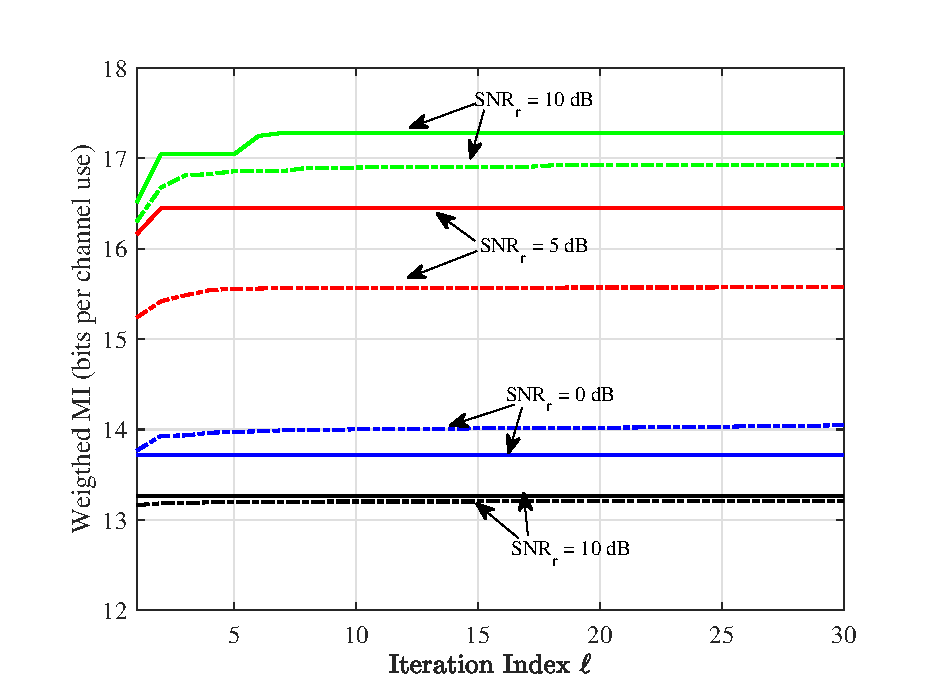
\includegraphics[width=1\columnwidth]{tsp_convergence_snr_nolegend.eps}
			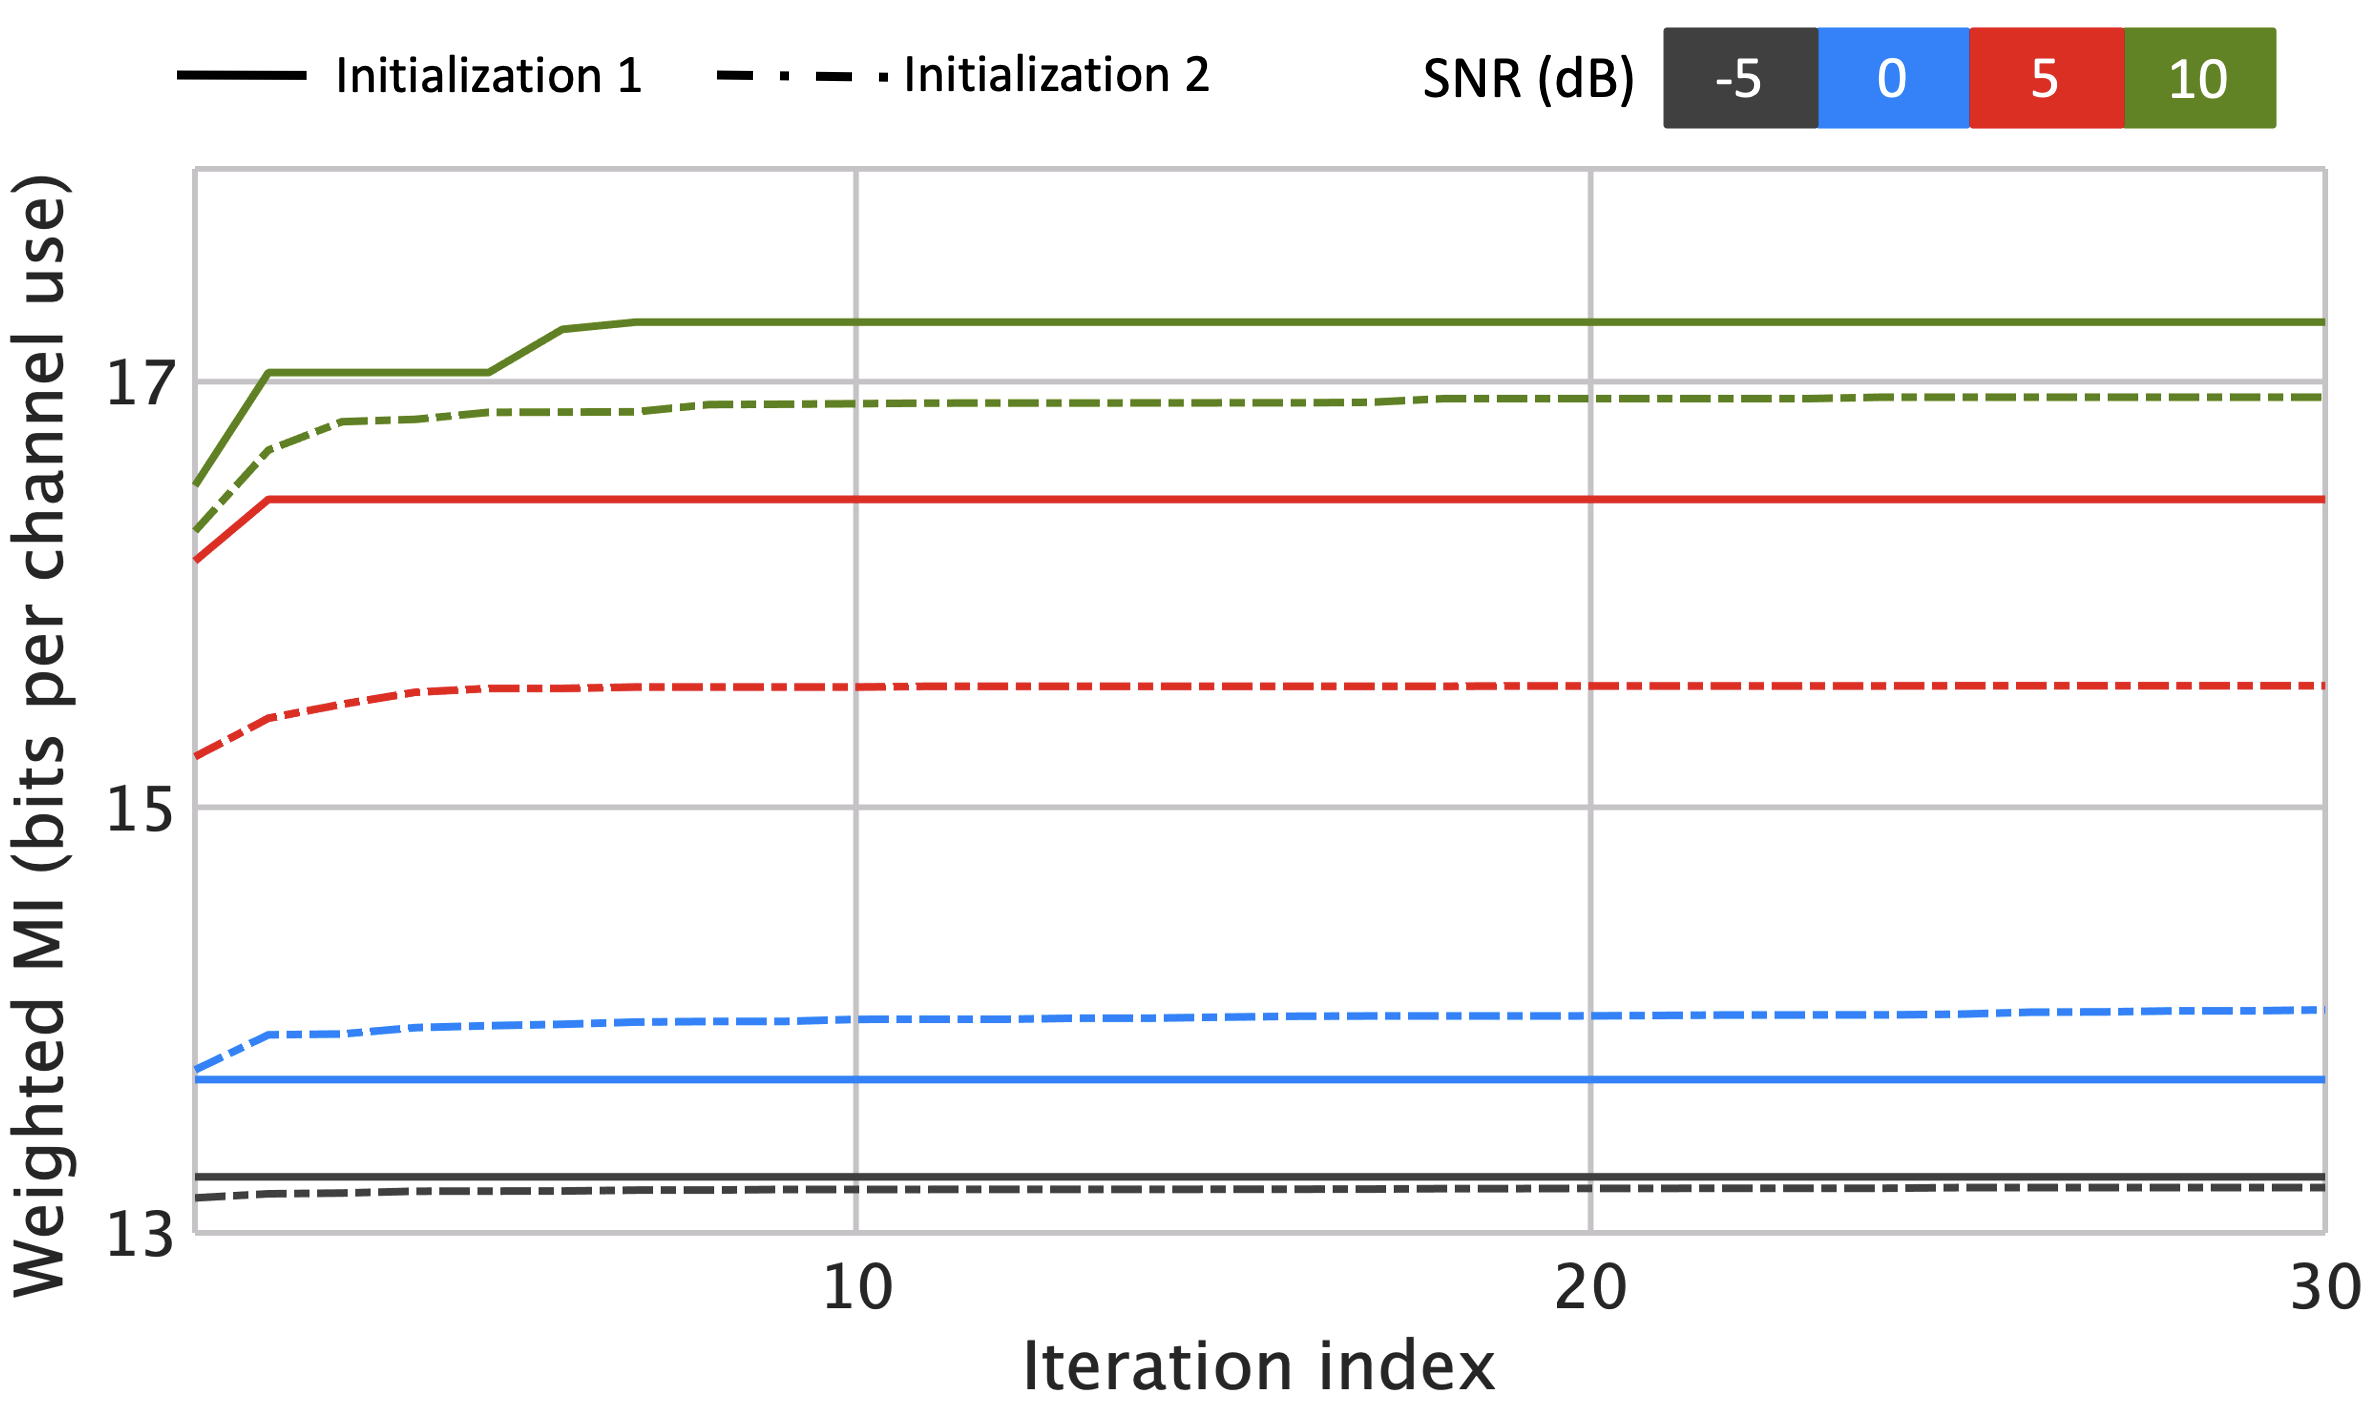
\includegraphics[width=1.0\columnwidth]{tsp_convergence_v03.png}
			%\vspace{-pt}
			\caption{Convergence behaviors of the BCD-AP MRMC algorithm with two initialization methods and multiple $\mathrm{SNR}_\textrm{r}$ values.}
			\label{fig:convergence}
			%\vspace{-1em}
		\end{figure}
		\iffalse
		\begin{figure}[!ht]
			\centering
			\subfloat[$\mathrm{SNR}_\textrm{r}=0\textrm{ dB}$ ]{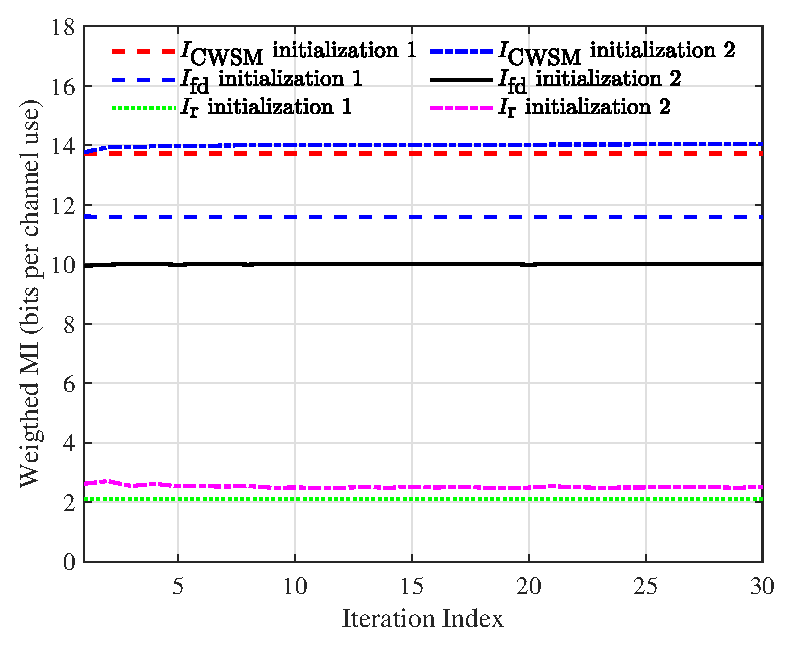
\includegraphics[width=0.45\linewidth]{tsp_convergence_0dB.eps}
				\label{fig: con_0dB}}
			\hfil
			\subfloat[$\mathrm{SNR}_\textrm{r}=10\textrm{ dB}$]{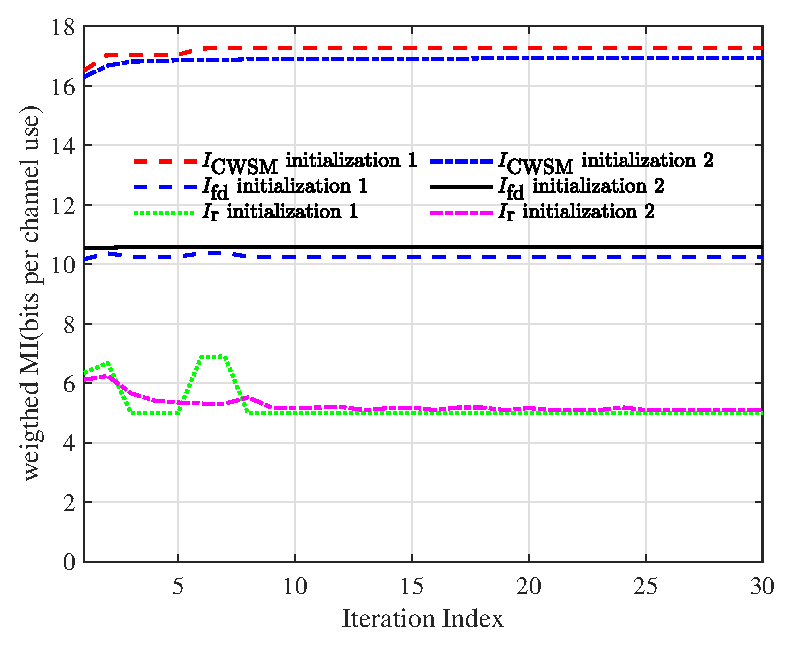
\includegraphics[width=0.45\linewidth]{tsp_convergence_10dB.eps}
				\label{fig: con_5dB}}
			\caption{Convergence behaviors of Algorithm $\ref{Alternating_sum}$ with two initialization methods}
			\label{fig: convergence}
			%\vspace{-1em}
		\end{figure}
		\fi
		%\vspace{-1em}
		\subsection{Radar Detection Performance}
		%-------------------------------------------------------------
		\begin{figure}[t]
			%\vspace{-1em}
			\centering
			%\subfloat[$\mathit{P}_{\textrm{d}}$ versus $\nu$ ]{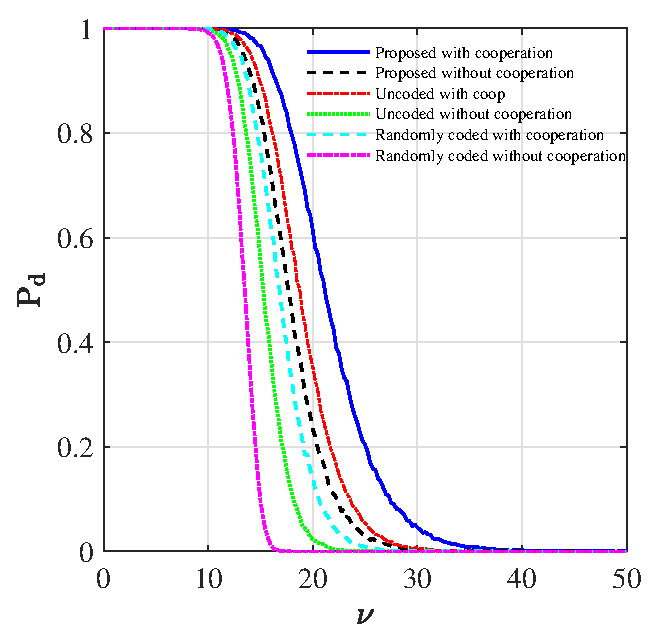
\includegraphics[width=0.48\linewidth]{tsp_pd_vs_vu.eps}
			%\label{fig: pd_vs_vu}}
			%\hfil
			%\subfloat[ROC of the NP detector]{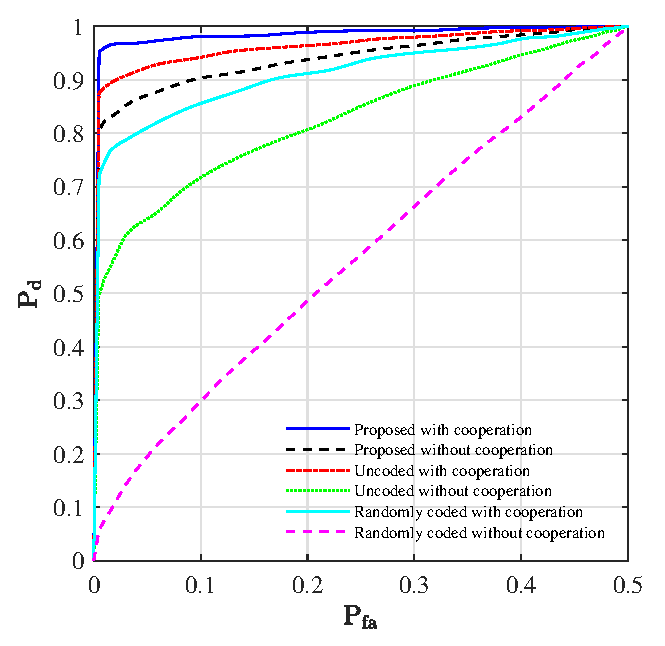
\includegraphics[width=0.48\linewidth]{tsp_ROC.eps}
			%\label{fig: roc}}
			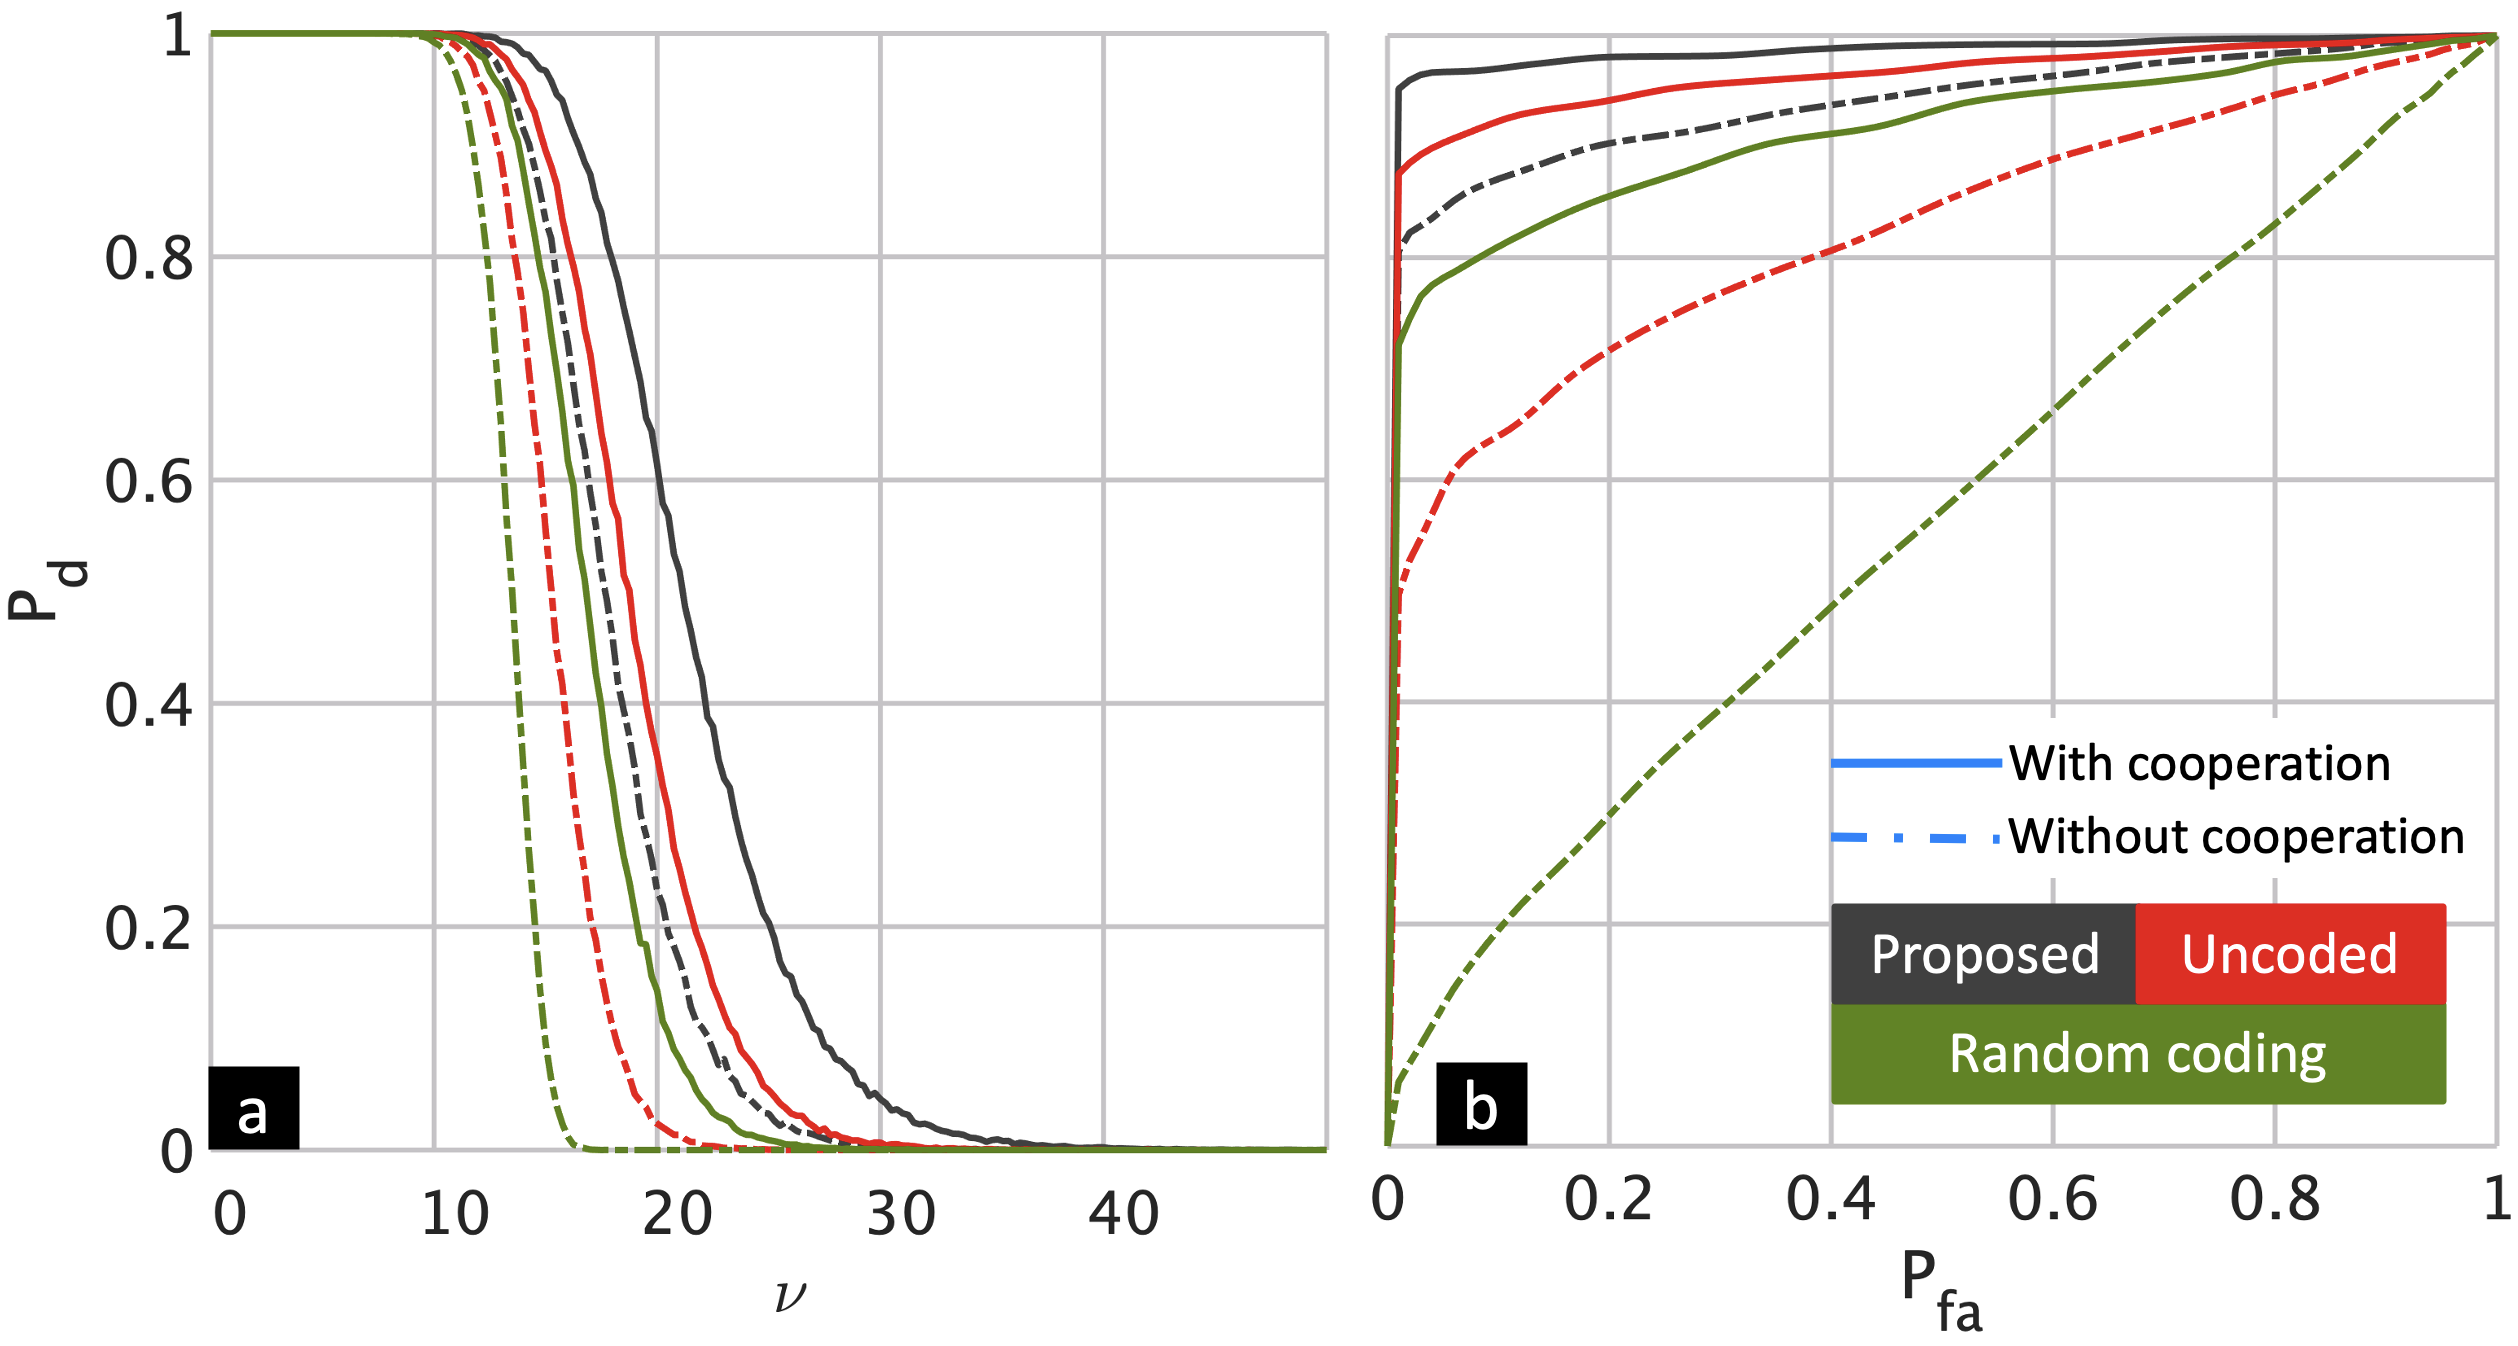
\includegraphics[width=1.0\columnwidth]{NPdetector.png}
			\caption{Target detection performance of the co-designed system compared with other radar codes and cooperation schemes using the NP detector. (a) $\mathit{P}_{\textrm{d}}$ versus $\nu$ (b) ROC of the NP detector.}
			\label{fig: NPdetector}
			%\vspace{-1em}
		\end{figure}
		%-------------------------------------------------------------
		We investigated the detection performance of the statistical MIMO radar using the designed code matrix $\mathbf{A}$. % based on a Newman-Pearson (NP) detector. 
		Consider the binary hypothesis testing formulation for target detection as
		\par\noindent\small
		\begin{equation}
			\label{eq: hypothesis1}
			\begin{cases}
				\mathcal{H}_{\mathrm{0}}: & \mathbf{y}_{\textrm{r}} = \mathbf{y}_{\textrm{cr}}+\mathbf{y}_{\textrm{Bmr}}+\mathbf{y}_{\textrm{Ur}}+\mathbf{z}_{\textrm{r}}
				\\
				\mathcal{H}_{\mathrm{1}}: & \mathbf{y}_{\mathrm{r}} = \mathbf{y}_{\textrm{tr}}+ \mathbf{y}_{\textrm{cr}}+\mathbf{y}_{\textrm{Bmr}}+\mathbf{y}_{\textrm{Ur}}+\mathbf{z}_{\textrm{r}},
			\end{cases}
		\end{equation}
		%$\mathbf{y}_{\textrm{cr}}=\bracket{\mathbf{y}^\top_{\textrm{c},1};\cdots;\mathbf{y}^\top_{\textrm{c},\mathit{N}\rr}}^\top$, $\mathbf{y}_{\textrm{Bmr}}=\bracket{\mathbf{y}^\top_{\textrm{Bm},1};\cdots;\mathbf{y}^\top_{\textrm{Bm},\mathit{N}\rr}}^\top$, $\mathbf{y}_{\textrm{Ur}}=\bracket{\mathbf{y}^\top_{\textrm{Ur},1};\cdots;\mathbf{y}^\top_{\textrm{Ur},\mathit{N}\rr}}^\top$, $\mathbf{z}_{\textrm{r}}=\bracket{\mathbf{z}^\top_{\textrm{r},1};\cdots;\mathbf{z}^\top_{\textrm{r},\mathit{N}\rr}}^\to p$, and $\mathbf{y}_{\textrm{tr}}=\bracket{\mathbf{y}^\top_{\textrm{tr},1};\cdots;\mathbf{y}^\top_{\textrm{tr},\mathit{N}\rr}}^\top$.  whose CMs can be written as  $\mathbf{R}_{t}=\oplus_{n\rr=1}^{\mathit{N}\rr}\mathbf{R}_{\textrm{t},n\rr}$, $\mathbf{R}_{\mathrm{c}}=\oplus_{n\rr}^{\mathit{N}\rr}$
		%Notice that the $\mathbf{y}_{\mathrm{c},\textrm{r}}$, $\mathbf{y}_{\mathrm{Bm}}$, $\mathbf{y}_{\mathrm{U}}$, and $\mathbf{z}$ are all zero mean Gaussian random vectors  with CMs being $\mathbf{R}_{t}=\oplus_{n\rr=1}^{\mathit{N}\rr}\mathbf{R}_{\textrm{t},n\rr}$, $\mathbf{R}_{\mathrm{c}}=\oplus_{n\rr}^{\mathit{N}\rr}$.
		where $\mathbf{y}_{\mathrm{r}}=\bracket{\mathbf{y}^\top_{\textrm{r},1};\cdots;\mathbf{y}^\top_{\textrm{r},\mathit{N}\rr}}^\top$ and $\mathbf{y}_{\textrm{tr}}=\bracket{\mathbf{y}^\top_{\textrm{tr},1};\cdots;\mathbf{y}^\top_{\textrm{tr},\mathit{N}\rr}}^\top$. Denote $\mathbf{y}^{\textrm{in}}_{\textrm{r}}\triangleq\mathbf{y}_{\textrm{cr}}+\mathbf{y}_{\textrm{Bmr}}+\mathbf{y}_{\textrm{Ur}}+\mathbf{z}_{\textrm{r}}=\bracket{\paren{\mathbf{y}^{\textrm{in}}_{\textrm{r},1}}^\top;\cdots;\paren{\mathbf{y}^{\textrm{in}}_{\textrm{r},N\rr}}^\top}^\top$ with its CM $\mathbf{R}^{\textrm{in}}_{\textrm{r}}=\oplus_{n\rr=1}^{N\rr}\mathbf{R}_{\textrm{in},n\rr}\in\mathbb{C}^{KN\rr\times KN\rr}$. We also define $\overline{\mathbf{y}}_{\textrm{r},n\rr} = \paren{\mathbf{R}^{\textrm{in}}_{\textrm{r},n\rr}}^{-\sfrac{1}{2}}\mathbf{y}_{\textrm{r},n\rr}\in\mathbb{C}^{K}$ and its CM $\mathbf{G}_{n\rr}=\paren{\mathbf{R}^{\textrm{in}}_{\textrm{r},n\rr}}^{-\sfrac{1}{2}}\mathbf{R}_{\textrm{r},n\rr}\paren{\mathbf{R}^{\textrm{in}}_{\textrm{r},n\rr}}^{-\sfrac{1}{2}}$. Rewrite problem \eqref{eq: hypothesis1} as  \par\noindent\small
		%If $\mathbf{M}_{n\rr}\triangleq\mathbf{R}_{\textrm{in},n\rr }$ and  , the test problem can be rewritten as 
		\begin{equation}
			\label{eq: hypothesis2}
			\begin{cases}
				\mathcal{H}_{\mathrm{0}}: & \overline{\mathbf{y}}_{\mathrm{r}}\sim\mathcal{CN}\paren{\mathbf{0},\mathbf{I}}
				\\
				\mathcal{H}_{\mathrm{1}}: & \overline{\mathbf{y}}_{\mathrm{r}}\sim\mathcal{CN}\paren{\mathbf{0},\mathbf{I}+\mathbf{G}},
			\end{cases}
		\end{equation}\normalsize
		where the block diagonal matrix $\mathbf{G}=\oplus_{n\rr=1}^{\mathit{N}\rr}\mathbf{G}_{n\rr}$. The eigendecomposition of $\mathbf{G}_{n\rr}$ is $\mathbf{G}_{n\rr}=\mathbf{V}_{n\rr}\mathbf{\Lambda}_{n\rr}\mathbf{V}^\dagger_{n\rr}$, where the columns of $\mathbf{V}_{n\rr}$ and the diagonal entries of $\mathbf{\Lambda}_{n\rr}\triangleq\diag\bracket{\delta_{1,n\rr},\cdots,\delta_{\mathit{K},n\rr}}$ are, respectively, the eigenvectors and eigenvalues of $\mathbf{G}_{n\rr}$, the $\ith{k}$ eigenvalue being $\delta_{k,n\rr}$. Using the Woodbury matrix identity and the eigendecomposition of $\mathbf{G}_{n\rr}$, the test statistic is\par\noindent\small
		\begin{flalign}
			T\paren{\overline{\mathbf{y}}}&=\sum_{n\rr=1}^{\mathit{N}\rr}T\paren{\overline{\mathbf{y}}_{\textrm{r},n\rr}}=\sum_{n\rr=1}^{\mathit{N}\rr}\overline{\mathbf{y}}^\dagger_{\textrm{r},n\rr}\paren{\mathbf{I}-\paren{\mathbf{G}_{n\rr}+\mathbf{I}}^{-1}}\overline{\mathbf{y}}_{\textrm{r},n\rr}\nonumber\\
			&=\sum_{n\rr=1}^{\mathit{N}\rr}\overline{\mathbf{y}}^\dagger_{\textrm{r},n\rr}\mathbf{V}_{n\rr}\paren{\mathbf{\Lambda}^{-1}+\mathbf{I}}^{-1}\mathbf{V}^\dagger_{n\rr}\overline{\mathbf{y}}_{\textrm{r},n\rr}
		\end{flalign}\normalsize
		Denote $\widehat{\mathbf{y}}_{\textrm{r},n\rr}=\mathbf{V}^\dagger_{n\rr}\overline{\mathbf{y}}_{\textrm{r},n\rr}=\bracket{\widehat{y}_{n\rr}\bracket{1},\cdots,\widehat{y}_{n\rr}\bracket{\mathit{K}}}$. Then, the Neyman-Pearson (NP) detector is\cite{Kay1993detection}
		\begin{equation}
			\label{eq: NPdetector}
			%\sum_{n\rr}^{\mathit{N}\rr}T\paren{\overline{\mathbf{y}}_{\textrm{r},n\rr}}
			T\paren{\overline{\mathbf{y}}}=\sum_{n\rr=1}^{\mathit{N}\rr}\sum_{k=1}^{\mathit{K}}\frac{\delta_{k,n\rr}\lvert\widehat{y}_{n\rr}\bracket{k}\rvert^2}{1+\delta_{k,n\rr}}\underset{\mathrm{H}_2}{\overset{\mathrm{H}_1}{\gtrless}}\nu,
		\end{equation}
		where $\nu$ is the threshold selected to guarantee a certain detection performance. We performed Monte Carlo (MC) simulations to evaluate the probability of detection $\mathit{P}_{\textrm{d}}$ and the Rx operating characteristic (ROC) (curve of $\mathit{P}_{\textrm{d}}$ versus probability of false alarm $\mathit{P}_{\textrm{fa}}$) of the NP detector. Figures~\ref{fig: NPdetector}a and \ref{fig: NPdetector}b show $\mathit{P}_{\textrm{d}}$ with respect to $\nu$ and ROC, %, namely the curve of $\mathit{P}_{\textrm{d}}$ versus the probability of false alarm $\mathit{P}_{\textrm{fa}}$, 
		respectively, for various coding schemes and cooperation modes. Here, presence or absence of cooperation indicates whether or not the DL signals $\mathbf{y}_{\textrm{Bt},n\rr}$ are incorporated in $\mathbf{y}_{\textrm{t,}n\rr}$ for all $n\rr$. For the $\ith{m\rr}$ radar Tx, the uncoded waveform is $\mathbf{a}_{m\rr}=\sqrt{\frac{\mathit{P}_{\textrm{r},m\rr}}{\mathit{K}}}\mathbf{1}_{\mathit{K}}$ and randomly coded waveform is  $\mathbf{a}_{m\rr}=\sqrt{\frac{\mathit{P}_{\textrm{r},m\rr}}{\mathit{K}}}\mathbf{u}_{m\rr}$, where $\braces{\mathbf{u}_{m\rr}}$ is a unitary basis. We generated $5000$ realizations of $\overline{\mathbf{y}}_{\textrm{r}}$ under hypothesis $\mathcal{H}_1$ to estimate $\mathit{P}_{\textrm{d}}$ and $\mathcal{H}_0$ to estimate $\mathit{P}_{\textrm{fa}}$ based on $\nu$ for each mode. Figures~\ref{fig: NPdetector}a and \ref{fig: NPdetector}b illustrate that our optimized radar code matrix outperforms the all-ones (uncoded) and random coding schemes, and that the cooperation between the radar and BS boosts the radar detection performance. For example, in , with $P_{\textrm{fa}}=0.1$, when radar codes and UL/DL precoders obtained via Algorithm \ref{Alternating_sum} are used along with radar-DL cooperation, this yields approximately $8\%$ improvement in $P_{\textrm{d}}$ over the non-cooperation mode, $6\%$ over the all-ones code with cooperation, and $13\%$ over random code with cooperation. We observe that even without the cooperation, our algorithm enables the MIMO radar to provide a competitive detection performance.
		
		\iffalse
		\begin{figure}[t]
			\centering
			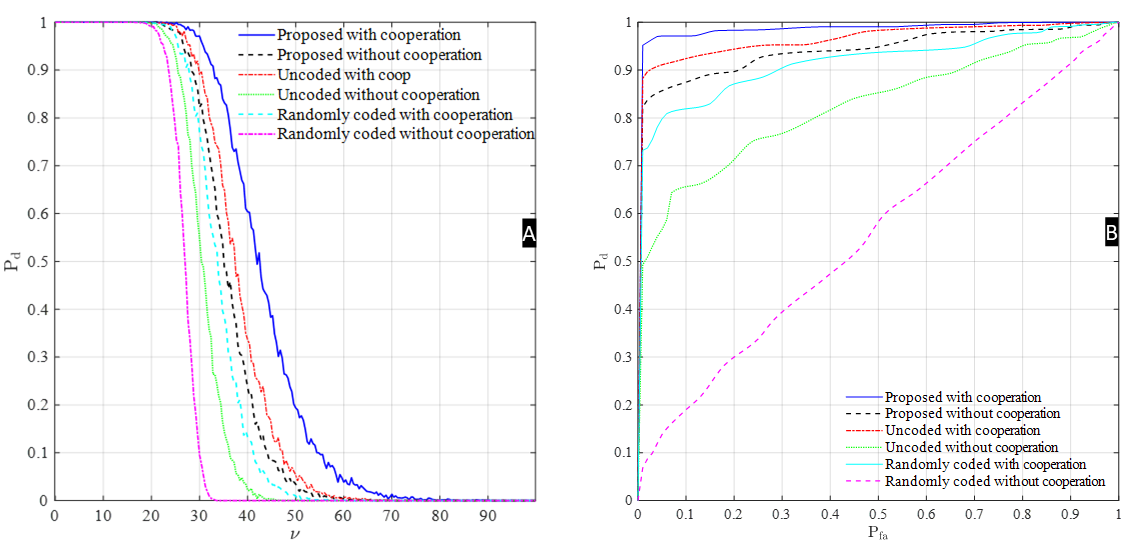
\includegraphics[width=0.45\linewidth]{radar_figures_roc.png}
			%\vspace{-14pt}
			\caption{$\paren{\textrm{a}}$ $\mathit{P}_{\textrm{d}}$ versus $\nu$ with different combinations of \textcolor{red}{coding schemes and cooperation modes} $\paren{\textrm{b}}$ the corresponding ROC of the NP detector}
			\label{fig: NPdetector}
		\end{figure}
		\fi
		%\vspace{-1em}
		\subsection{FD Communications Performance}
		\label{subsec: fd_comm_eva}
		\begin{figure}[t]
			%\vspace{-1em}
			\centering
			%\subfloat[Weighted MI versus various number of UL UEs]{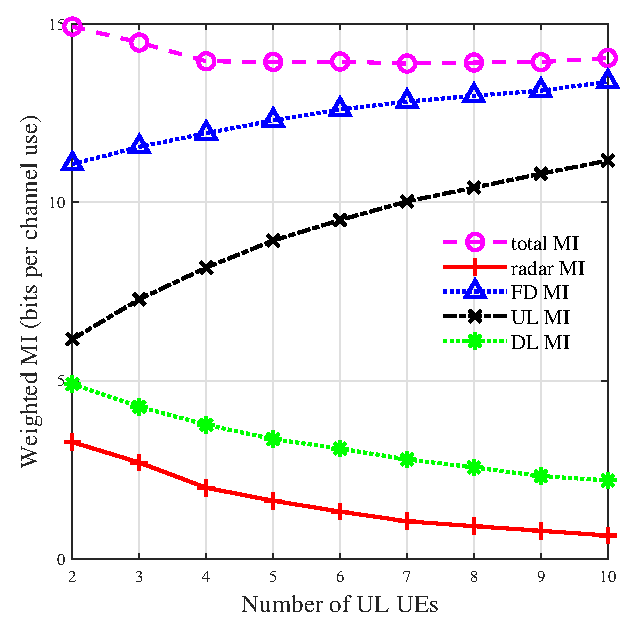
\includegraphics[width=0.48\linewidth]{II.eps}
			%\label{fig: UL_UE}}
			%\hfil
			%\subfloat[Weighted MI versus various number of DL UEs]{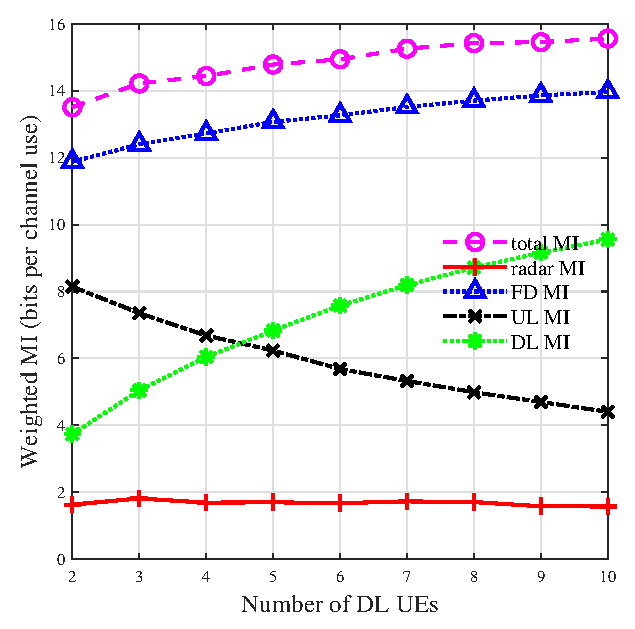
\includegraphics[width=0.48\linewidth]{tsp_DL_UE.eps}
			%\label{fig: DL_UE}}
			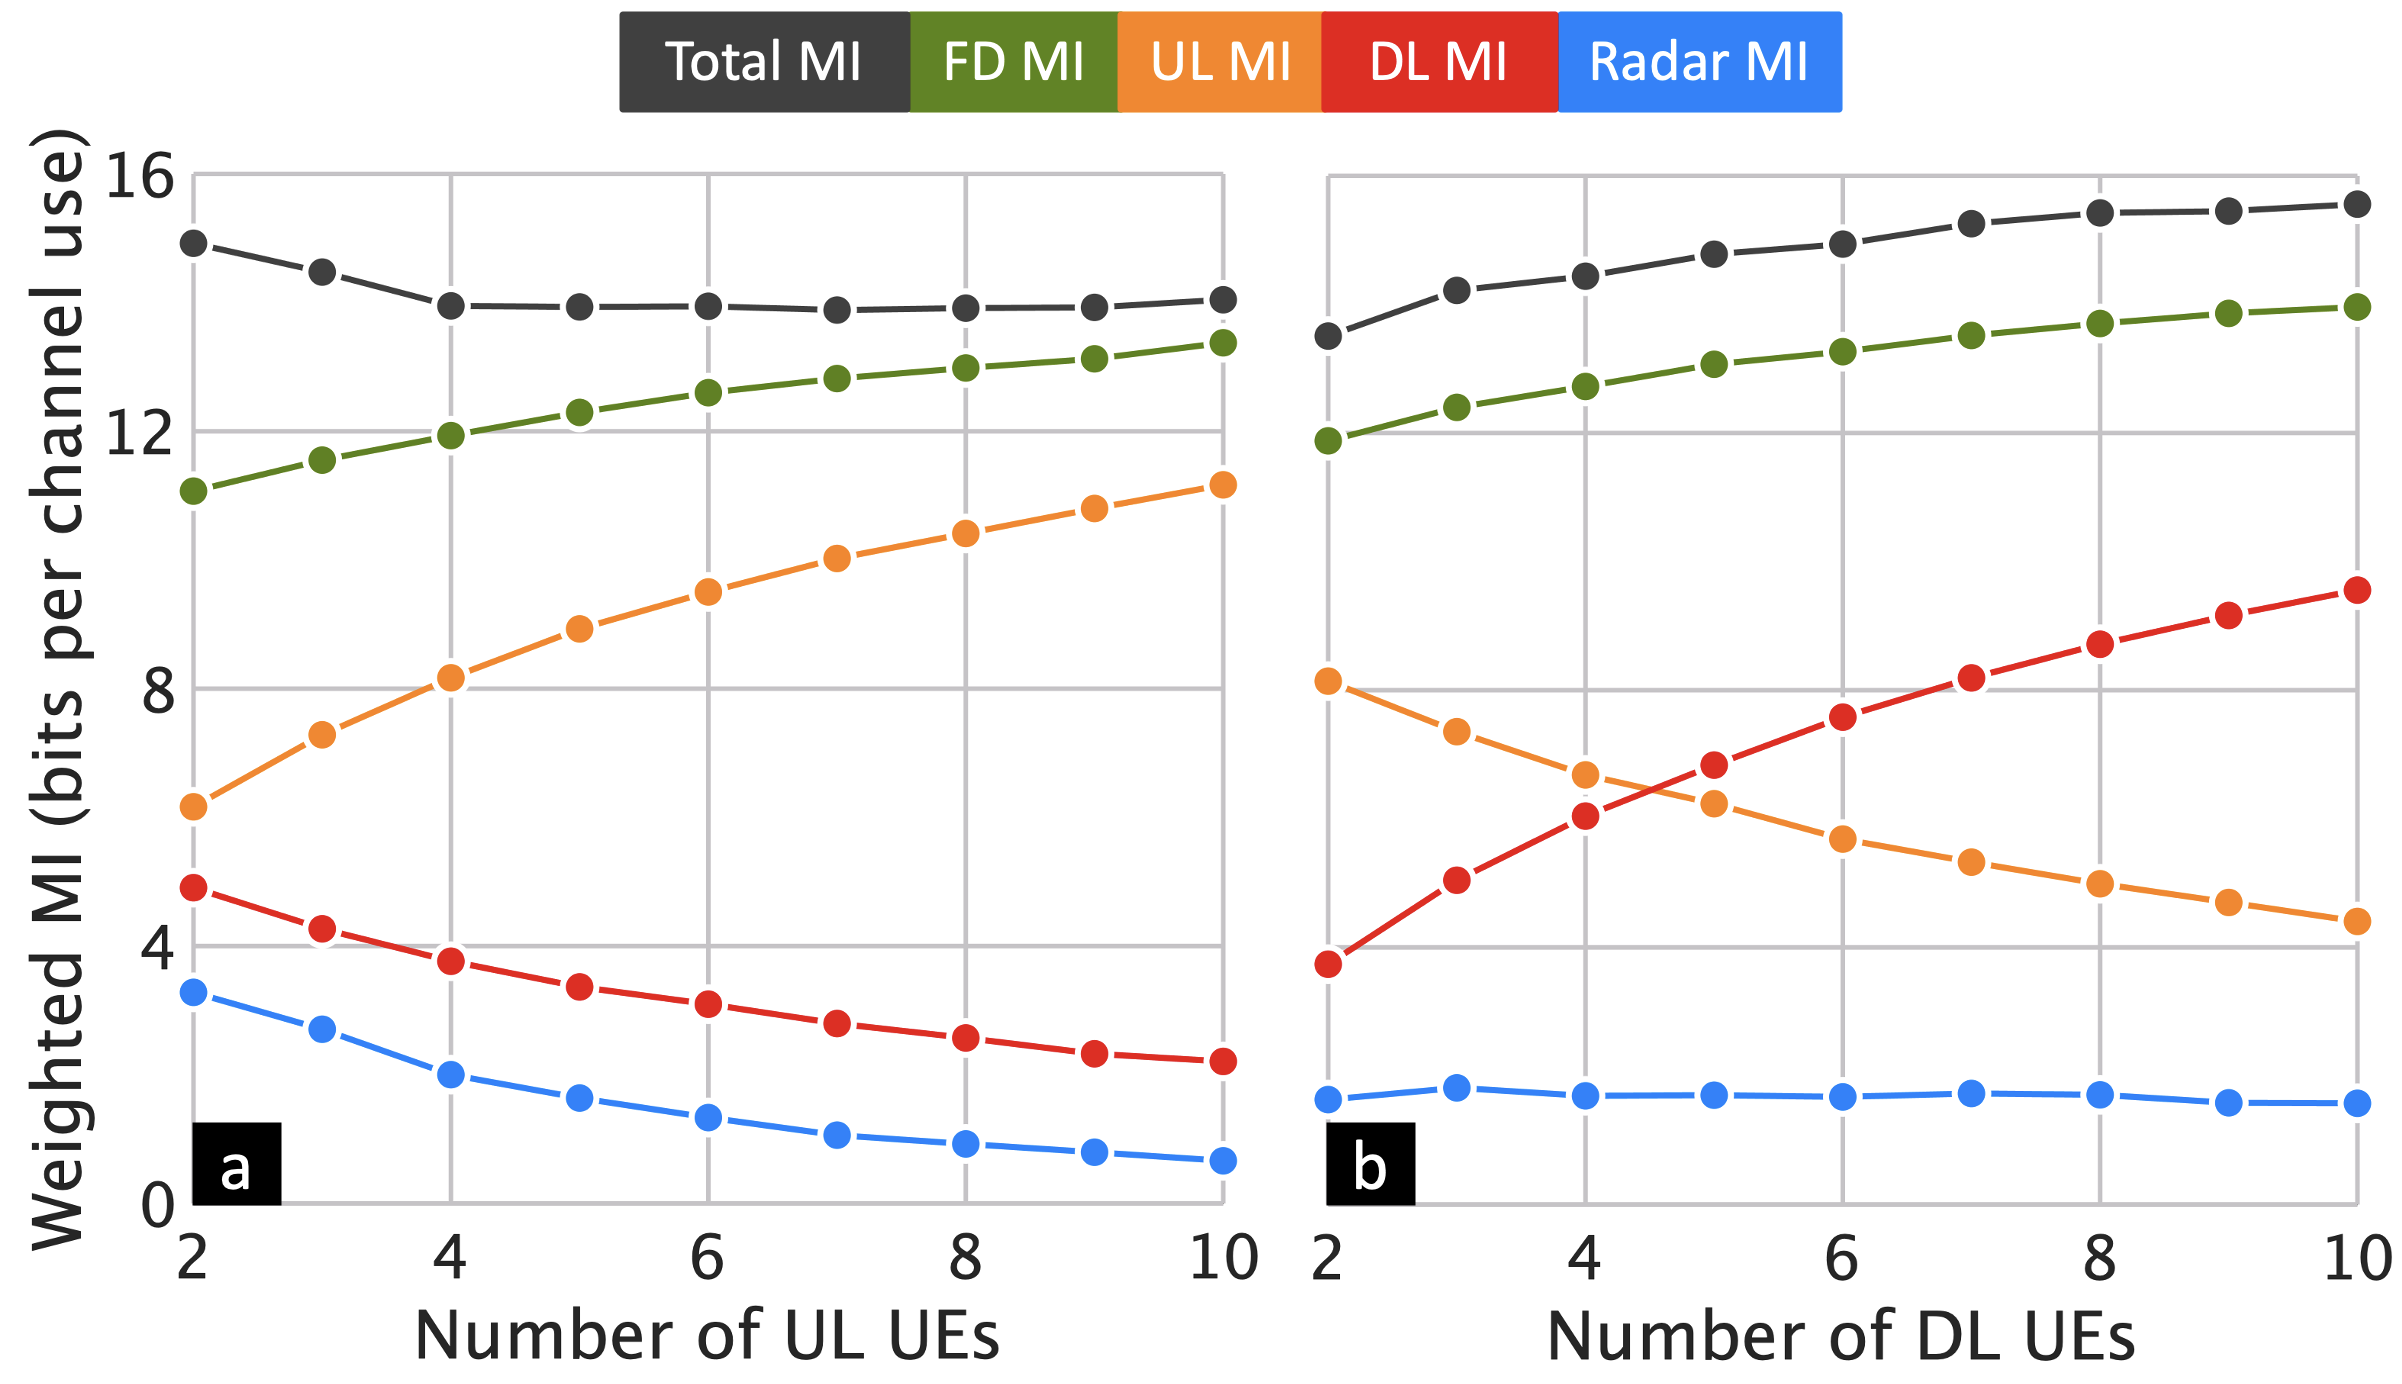
\includegraphics[width=0.9\columnwidth]{fd_UE.png}
			\caption{Performance of the co-designed system compared with increasing numbers of (a) UL and (b) DL UEs.}
			\label{fig:fd_UE}
			%\vspace{-1em}
		\end{figure}
		%-------------------------------------------------------------
		We explored the effect on the system performance with increasing UEs. Figures~\ref{fig:fd_UE}a and \ref{fig:fd_UE}b depict weighted UL MI $\mathit{I}_{\textrm{U}}\triangleq\sum_{k}\sum_{i}\alpha^\textrm{u}_i\mathit{I}_{\mathrm{u},i}\bracket{k}$, weighted DL MI $\mathit{I}_{\textrm{D}}\triangleq\sum_{k}\sum_{j}\alpha^\textrm{d}_j\mathit{I}_{\mathrm{d},j}\bracket{k}$, radar MI $\mathit{I}_{\textrm{R}}\triangleq\alpha^\textrm{r}_{n\rr}\sum_{n\rr}\mathit{I}_{\textrm{r},n\rr}\bracket{k}$, total weighted FD MI and $\mathit{I}_{\textrm{CWSM}}$ as the number of UL UEs and DL UEs are varied, respectively. The power levels are set at $\mathit{P}_{\textrm{u}}=I$ and $\mathit{P}_{\textrm{d}}=J$. As the number of UL UEs 
		increases from $\mathit{I}=2$ to $\mathit{I}=10$ with the number of DL UEs fixed at $\mathit{J}=2$, the performances of DL UEs and radar Rxs deteriorate owing to the increasing UL interference. On the other hand, the performance of the UL drops while that of the MIMO radar remains relatively stable as the number of DL UEs rises from $\mathit{J}=2$ to $\mathit{J}=10$ with $\mathit{I}=2$. We observe that the total system performance measure  $\mathbf{I}_{\textrm{CWSM}}$ is enhanced with a higher DL power because of the radar-DL cooperation whereas $\mathbf{I}_{\textrm{CWSM}}$ declines with a rising UL power. 
		
		%\vspace{-1em}
		\subsection{Joint Radar-Communications Performance}
		%-------------------------------------------------------------
		\begin{figure}[t]
			\centering
			%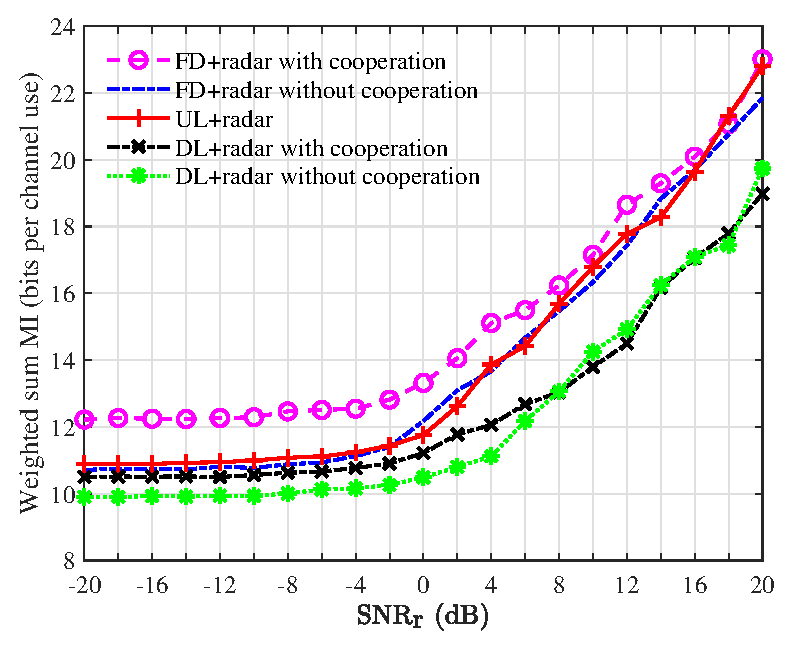
\includegraphics[width=1\columnwidth]{fd_vs_hd.eps}
			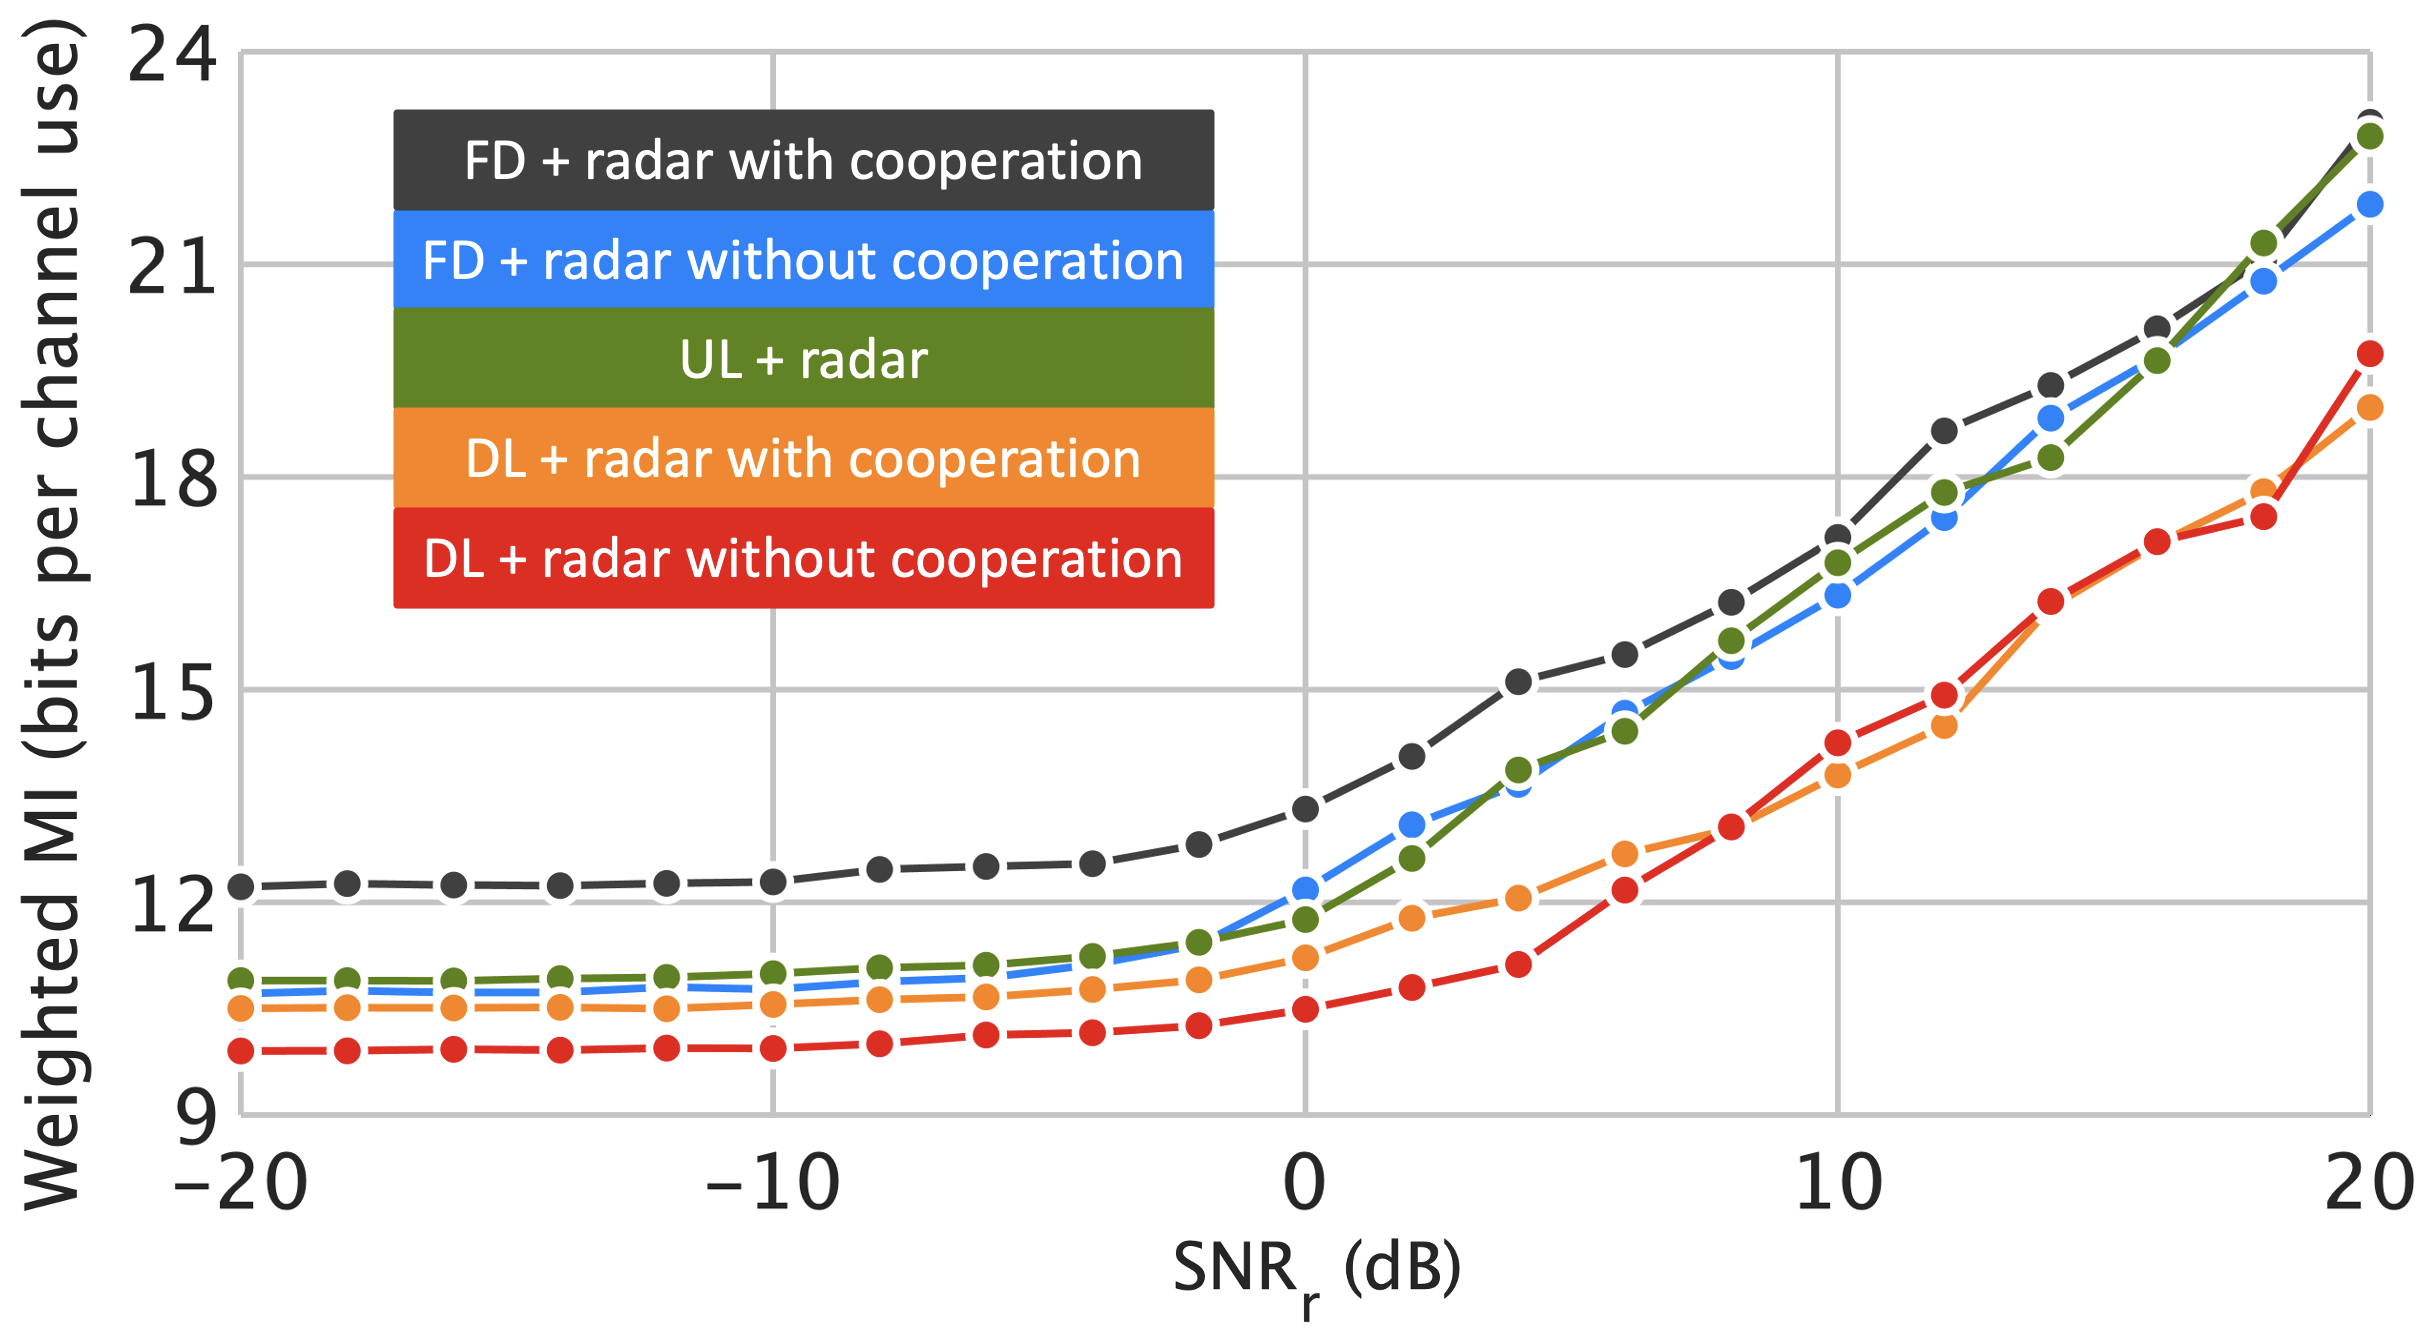
\includegraphics[width=1.0\columnwidth]{fd_vs_hd_v03.png}
			%\vspace{-pt}
			\caption{Evaluation of the MU-MIMO communications with different transmission schemes under various radar SNRs}
			\label{fig:fd_vs_hd}
			%\vspace{-1em}
		\end{figure}
		%-------------------------------------------------------------
		\begin{figure}[t]
			\centering
			%\subfloat[System performance vs UL SNRs]{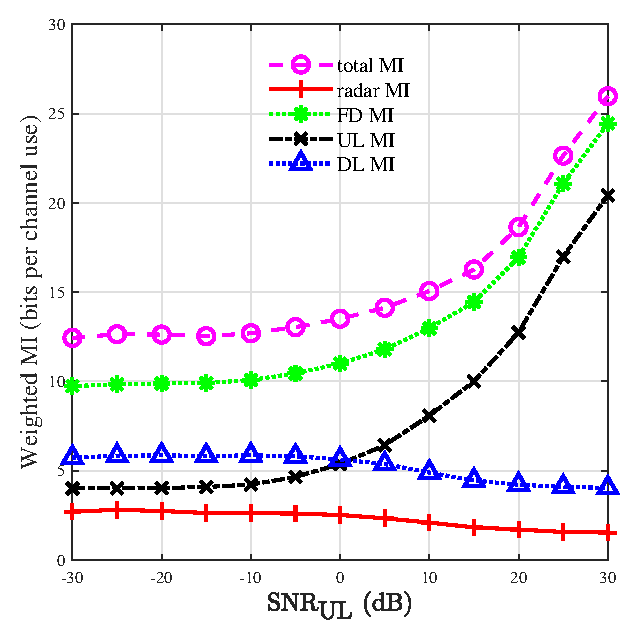
\includegraphics[width=0.48\columnwidth]{UL_SNR_sweep.eps}
			%\label{fig: UL_SNR}}
			%\hfil
			%\subfloat[System performance vs CNR]{\includegraphics[width=0.48\columnwidth]{CNR_sweep.eps}
			%\label{fig: CNR}}
			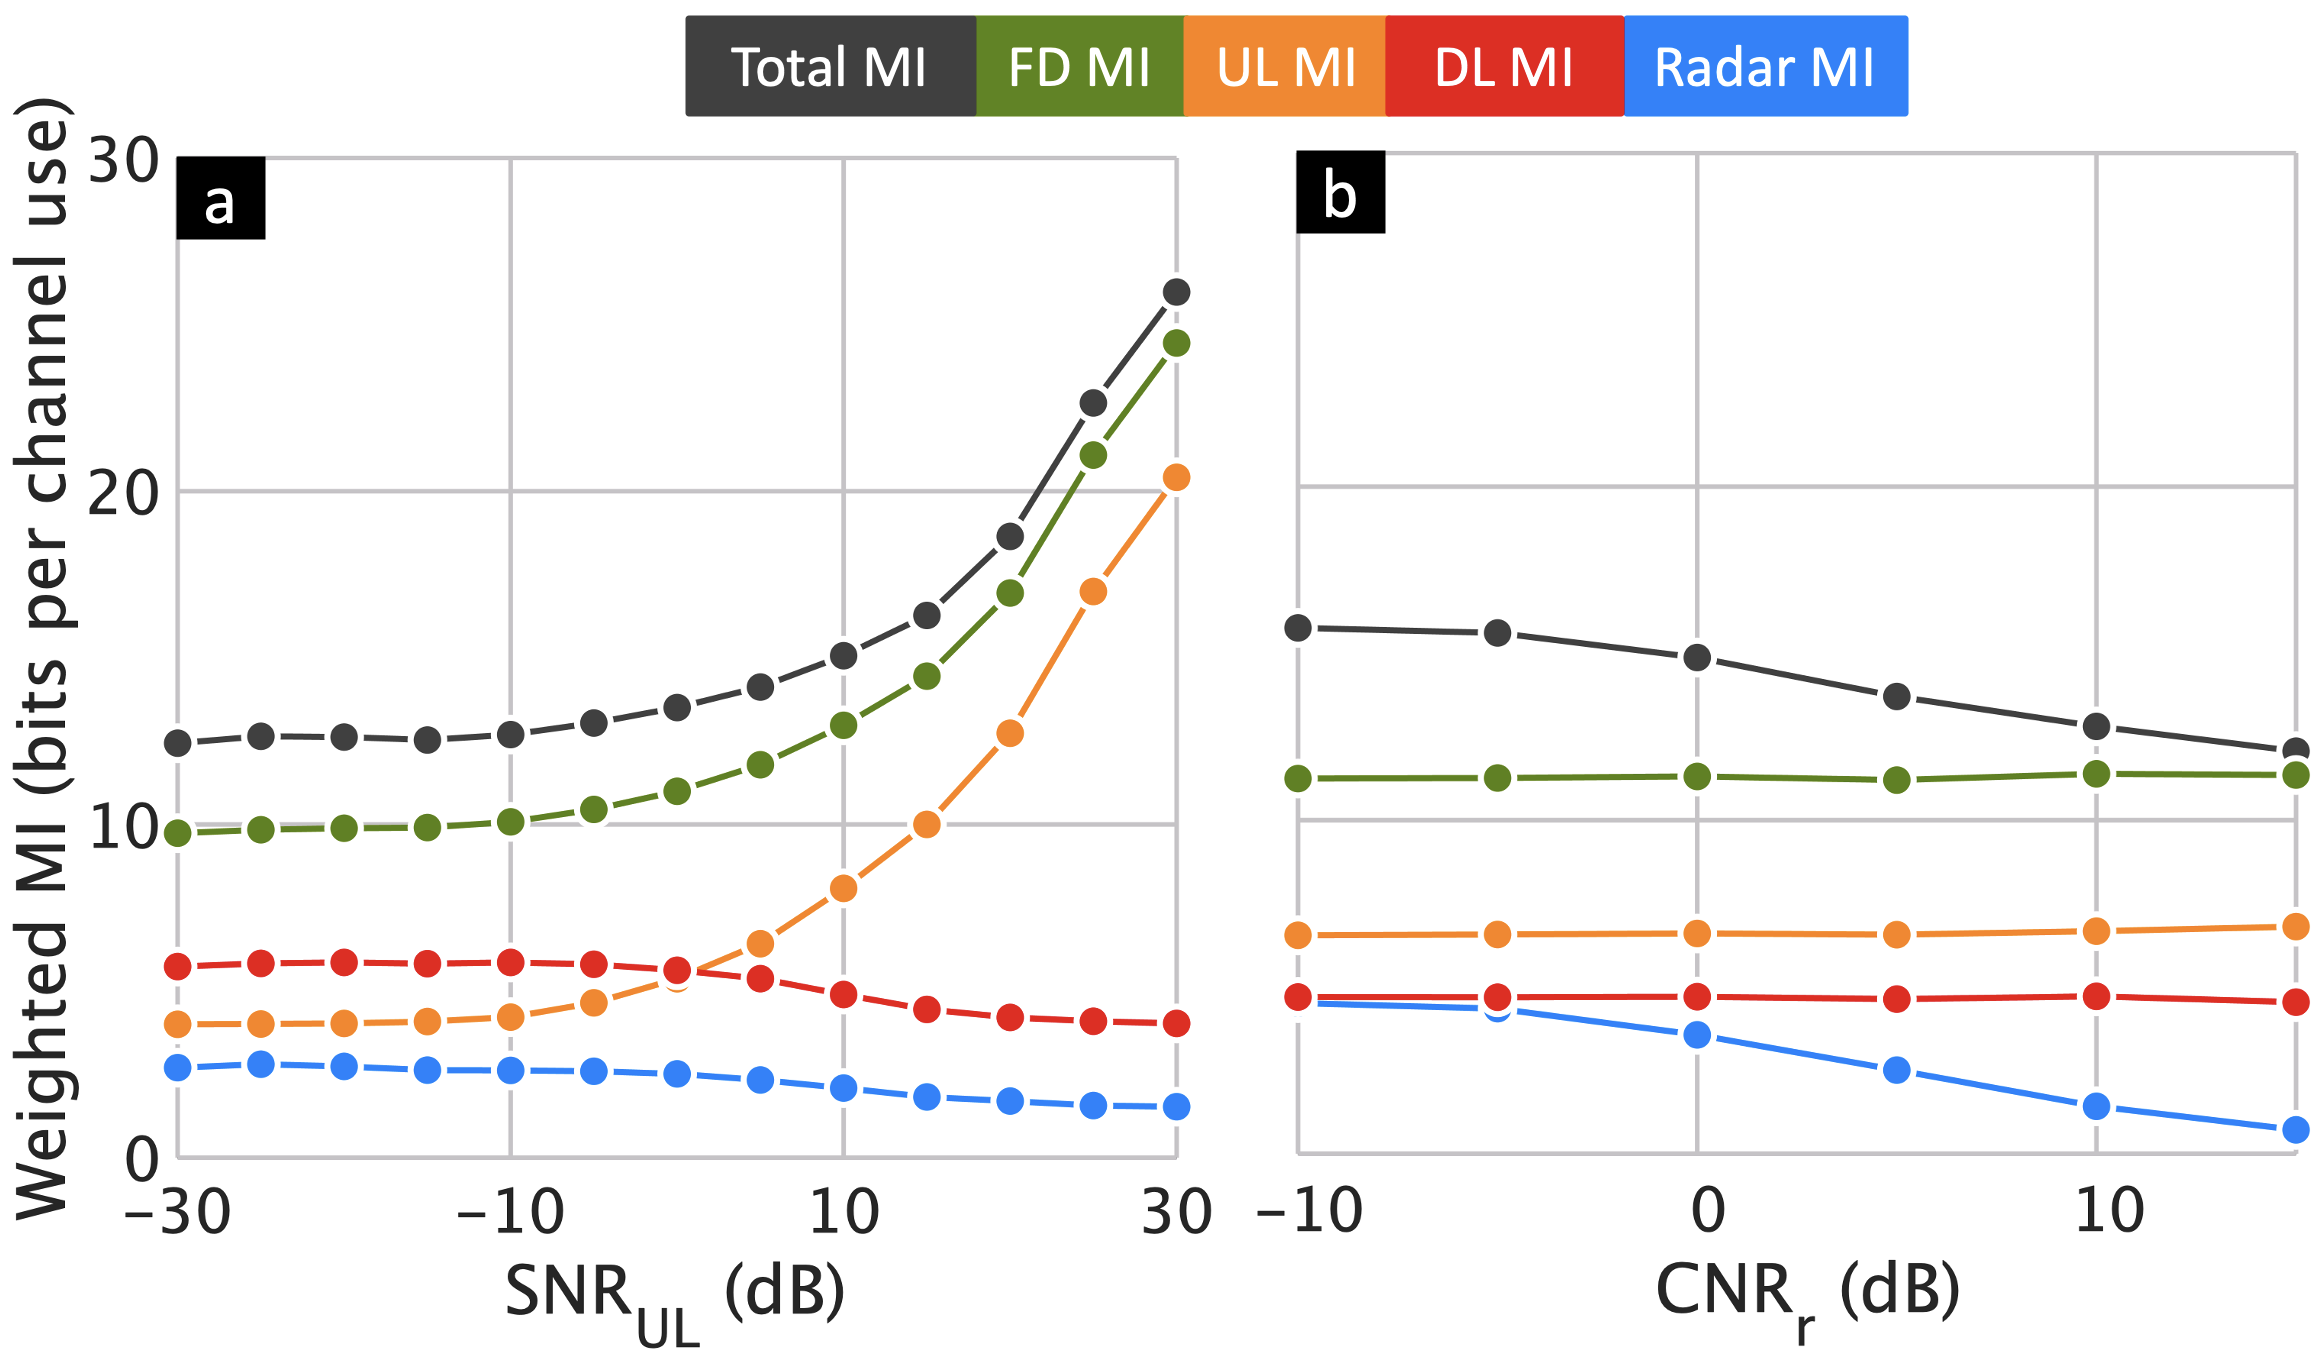
\includegraphics[width=0.9\columnwidth]{joint.png}
			\caption{Joint radar and communications interference analysis. (a) System performance vs UL SNRs (b) System performance vs CNR.}
			\label{fig:joint}
			%\vspace{-1em}
		\end{figure}
		\iffalse
		%-------------------------------------------------------------
		\begin{figure}[t]
			\centering
			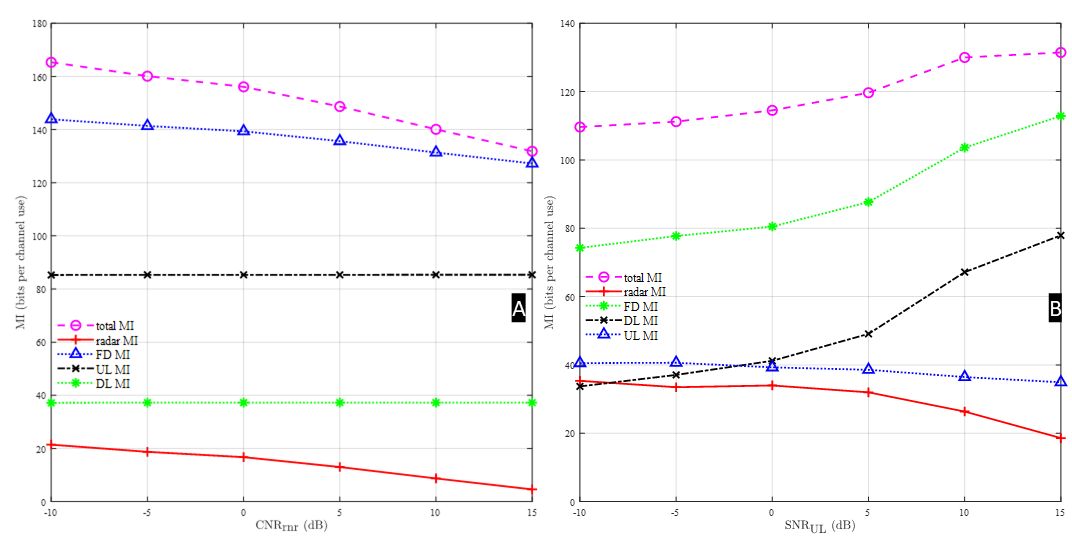
\includegraphics[width=1\columnwidth]{radar_figures_cnr.png}
			%\vspace{-14pt}
			\caption{$\paren{\textrm{a}}$ MI achieved by Algorithm $\ref{Alternating_sum}$ versus different $\mathrm{CNRs}$   $\paren{\textrm{b}}$ MI achieved by Algorithm $\ref{Alternating_sum}$ versus various UL $\mathrm{SNR}$ }
			\label{fig:cnr}
			%\vspace{-1em}
		\end{figure}
		%-------------------------------------------------------------
		\fi
		Finally, we evaluated the co-design performance by observing the mutual impact of the statistical MIMO radar and IBFD MU-MIMO communications on each other. Figure~\ref{fig:fd_vs_hd} compares the CWSMs achieved by the IBFD MU-MIMO as well as the HD MU-MIMO communications jointly operating with a statistical MIMO radar. We also included the cooperation and non-cooperation modes for IBFD MU-MIMO and DL MU-MIMO communications. In practice, the radar-enabled interference channel gains, namely $\eta^2_{\mathrm{r},j}$ and $\eta^2_{\mathrm{rB}}$ are fractions of the radar-target channel gains $\eta^2_{m\rr,n\rr}$. As a result, the severity of the radar-enabled interference with the communications systems are also related to the radar-target channel gains. Specifically, we set $\mathrm{SNR}_{\textrm{r}}=0.8\mathrm{SNR}_{\textrm{rB}}$ and $\mathrm{SNR}_{\textrm{r}}=0.6\mathrm{SNR}_{\textrm{rd}}$. We observed that when the radar power dominates the co-designed system, the impact of radar-DL cooperation is less apparent. In \figurename{\;\ref{fig:joint}}, the performance of co-designed system is shown to vary with different UL SNR and CNR values.  %Like the assumption we made with \figurename{\;\ref{fig:fd_vs_hd}}, 
		Here, $\mathrm{SNR}_{\textrm{ur}}=0.7\mathrm{SNR}_{\textrm{u}}$ and  $\mathrm{SNR}_{\textrm{ud}}=0.8\mathrm{SNR}_{\textrm{u}}$ for Fig.~\ref{fig:joint}a  and $\mathrm{SNR}_{\textrm{rB}}=0.5\mathrm{CNR}_{\textrm{r}}$ and $\mathrm{SNR}_{\textrm{rd}}=0.5\mathrm{CNR}_{\textrm{r}}$ for Fig.~\ref{fig:joint}b.  Note that the DL and radar weighted MIs decline by approximately $30\%$ and $45\%$, respectively, when the UL-DL and UL-radar interfering signal powers are $10^6$ times higher. This demonstrates that the designed precoders and radar codes sustain the DL and radar performances despite a high UL Tx power. Meanwhile, from Fig.~\ref{fig:joint}b, the clutter affects the MIMO radar more than the FD communications UEs because the proposed method mitigates the power projected to the interfering channels $\mathbf{H}_{\textrm{rB}}$ and $\mathbf{H}_{\textrm{r,}j}$ from $\braces{\mathbf{a}\bracket{k}}$.
		% $\eta_{\mathrm{u},i}$ and $\eta_{\mathrm{d},i}$ are fractions of $\eta^2_{i,n\rr}$ and $\eta_{m\rr,\B}$ and $\eta_{m\rr,j}$ are fractions of $\sigma^2_{\textrm{c},n\rr}$. 
		%\vspace{-1em}
		%\section{Conclusion}
		\section{Summary}
		\label{sec:conclusion}
		%\textcolor{red}{Need to make this shorter}
		In this work, we proposed a spectral co-design for a statistical MIMO radar and an IBFD MU-MIMO communications system. Prior works either largely consider co-located MIMO radars, focus on coexistence solutions, or partially analyze MIMO communications. We take a wholesome view of the problem by jointly designing several essential aspects of such a co-design:  UL/DL precoders, MIMO radar code matrix, and LRFs for both systems. Our proposed BCD-AP MRMC algorithm not only guarantees convergence but also provides performance benefits for both systems. %First, we demonstrate the rapid convergence of the BCD-AP MRMC algorithm with two different initializations. Second, 
		The radar codes generated by BCD-AP MRMC significantly increase the probability of detection over conventional coding schemes. We also showed that the cooperation between radar and DL signals is beneficial for target detection. The co-designed DL and radar are resilient to considerable UL interference. Similarly, using our optimized precoders and radar codes, the DL and UL rates remain stable as the CNR is increased. %Based on our theoretical and numerical results, we conclude that our algorithm is a superior approach to achieve the spectral co-design for the co-existence of a statistical MIMO radar and an IBFD MU-MIMO communications system. 
		%For the future work, we would address the impact of the CSI errors on both the MIMO radar and IBFD MU-MIMO communications and develop a robust version of the proposed framework.
		%such that the MIMO radar and the FD MU-MIMO communications system can operate simultaneously on the same spectrum while maintaining their respective performances.
		%  if have a single appendix:
		%\appendix[Proof of the Zonklar Equations]
		% or
		%\appendix  % for no appendix heading
		% do not use \section anymore after \appendix, only \section*
		% is possibly needed
		% use appendices with more than one appendix
		% then use \section to start each appendix
		% you must declare a \section before using any
		% \subsection or using \label (\appendices by itself
		% starts a section numbered zero.)
		%
		
		%\vspace{-1em}	
		\appendices
		\section{Proof of Theorem \ref{theorem: dual}}
		\label{appendix:theorem2}
		Solving $\paren{\ref{dualproblem}}$ yields the lower bounds of $\paren{\ref{WMMSE2}}$. The difference between the lower bound and the actual optimal value is the optimal duality gap. To equivalently obtain $\braces{\mathbf{P}^\star}$ and $\mathbf{A}^\prime$ with $\paren{\ref{dualproblem}}$, strong duality ought to hold for the primal problem $\paren{\ref{WMMSE1}}$, i.e., the optimal duality gap needs to be zero. However, the QoS constraints $\paren{\mathrm{\ref{UL_rate}}}-\paren{\mathrm{\ref{DL_rate}}}$ are non-concave leading to a non-zero duality gap. To bypass this problem, we apply the Taylor series to obtain linear approximations of $\mathit{R}_{\textrm{u},i}\bracket{k}$ and $\mathit{R}_{\textrm{d},j}\bracket{k}$. The first-order Taylor series expansion of a real-valued function with complex-valued matrix arguments $f\paren{\mathbf{X},\mathbf{X}^\ast}: \mathbb{C}^{\mathit{N}\times \mathrm{Q}}\times\mathbb{C}^{\mathit{N}\times \mathrm{Q}}\rightarrow\mathbb{R}$ around $\mathbf{X}_{\mathrm{0}}$ produces \cite{IMM2012-03274} \par\noindent\small
		\begin{flalign}
			\label{eq: Taylor}
			f\paren{\mathbf{X},\mathbf{X}^\ast} &= f\paren{\mathbf{X}_{\mathrm{0}},\mathbf{X}^\ast_{\mathrm{0}}}+\vect^\top\paren{\frac{\partial }{\partial \mathbf{X}_{\mathrm{0}}}f\paren{\mathbf{X}_{\mathrm{0}},\mathbf{X}^\ast_{\mathrm{0}}}}\vect\paren{\mathbf{X}-\mathbf{X}_{\mathrm{0}}}\nonumber\\
			&+\vect^\top\paren{\frac{\partial }{\partial \mathbf{X}^\ast_{\mathrm{0}}}f\paren{\mathbf{X}_{\mathrm{0}},\mathbf{X}^\ast_{\mathrm{0}}}}\vect\paren{\mathbf{X}^\ast-\mathbf{X}^\ast_{\mathrm{0}}}.
		\end{flalign}\normalsize
		based on their associated Taylor series expansions in the initial approximations %of, $\PBj$, and $\mathbf{a}\bracket{k}$, denoted by 
		$\widetilde{\mathbf{P}}_{\textrm{u},i}\bracket{k}$, $\widetilde{\mathbf{P}}_{\textrm{d},j}\bracket{k}$, and $\widetilde{\mathbf{a}}\bracket{k}$ Denoting $\widetilde{\mathbf{P}}_{\textrm{u},i}\bracket{k}$ as an initial approximation of $\PiB$, the Taylor series expansion of $\mathit{R}_{\textrm{u},q}\bracket{k}$ at $\widetilde{\mathbf{P}}_{\textrm{u},i}\bracket{k}$ gives \par\noindent\small
		\begin{IEEEeqnarray}{rCl}
			&&\mathit{R}_{\textrm{u},q}\bracket{k}\paren{\PiB}\approx \mathit{R}_{\textrm{u},q}\bracket{k}\paren{\widetilde{\mathbf{P}}_{\textrm{u},i}\bracket{k}}+\nonumber\\
			&&\vect\braces{\frac{\partial \paren{\mathit{R}_{\textrm{u},q}\bracket{k}\paren{\widetilde{\mathbf{P}}^\ast_{\textrm{u},i}\bracket{k}}}}{\partial \widetilde{\mathbf{P}}_{\textrm{u},i}\bracket{k}}}^\top\vect\braces{\PiB-\widetilde{\mathbf{P}}_{\textrm{u},i}\bracket{k}}+\nonumber\\
			&&\vect\braces{\frac{\partial \paren{\mathit{R}_{\textrm{u},q}\bracket{k}\paren{\widetilde{\mathbf{P}}_{\textrm{u},i}\bracket{k}}}}{\partial \widetilde{\mathbf{P}}^\ast_{\textrm{u},i}\bracket{k}}}^\top \vect\braces{\mathbf{P}^\ast_{\textrm{u},i}\bracket{k}-\widetilde{\mathbf{P}}^\ast_{\textrm{u},i}\bracket{k}}.
		\end{IEEEeqnarray}\normalsize
		Likewise, by defining $\widetilde{\mathbf{P}}_{\textrm{d},j}\bracket{k}$ and $\widetilde{\mathbf{a}}\bracket{k}$ as initial approximations of $\PBj$, and $\mathbf{a}\bracket{k}$, one can find the linear approximations of $\mathit{R}_{\textrm{u},q}\bracket{k}\paren{\PBj}$, $\mathit{R}_{\textrm{u},q}\bracket{k}\paren{\mathbf{a}\bracket{k}}$, $\mathit{R}_{\textrm{d},j}\bracket{k}\paren{\PiB}$, $\mathit{R}_{\textrm{d},m}\bracket{k}\paren{\PBj}$, and $\mathit{R}_{\textrm{d},j}\bracket{k}\paren{\mathbf{a}\bracket{k}}$. As $\Xi_{\text{wmmse}}$ is multi-convex, namely that $\Xi_{\text{wmmse}}$ is not jointly convex in $\PiB$, $\PBj$, and $\mathbf{a}\bracket{k}$ but convex in each individual variable provided the rest of the variables are fixed \cite{FD_WMMSE,BCDconvergence}, we thus have a fully convex approximation of \eqref{WMMSE2} in \eqref{dualproblem} and reduce the optimal duality gap between these two problems to zero \cite{Lui2006subg}, which concludes the proof.
		%the solutions to \eqref{WMMSE2}, $\braces{\mathbf{P}^\star}$ and $\mathbf{A}^\prime=\bracket{\paren{\mathbf{a}^\prime\bracket{1}}^\top,\cdots,\paren{\mathbf{a}^\prime\bracket{\mathit{K}}}^\top}$ can be equivalently solved through problem \eqref{dualproblem}. This concludes the proof.
		%\vspace{-1em}
		\section{Derivation of Gradients}
		\label{app:grad}
		Adopting the notations from \cite{IMM2012-03274}, we denote the complex gradient operator for a scalar real-valued function with a complex-valued matrix argument $f\paren{\mathbf{Z},\mathbf{Z^\star}}$ as $\nabla_\mathbf{Z}f=\frac{\partial f}{\partial\mathbf{Z}^\ast}$. From the derivative formula $\frac{\partial}{\partial \mathbf{X}^\ast}\trace\paren{\mathbf{B}^\top\mathbf{X}^\dagger\mathbf{CXB}}=\mathbf{C}^\top\mathbf{XBB}^\top+\mathbf{CXBB}^\top $ \cite{IMM2012-03274}, the gradients of $\Xi_{\text{UL}}$ and $\Xi_{\text{DL}}$ w.r.t. $\PiB$, $\PBj$ and $\mathbf{a}\bracket{k}$, respectively, are \par\noindent\small
		%\begin{flalign}
		\begin{IEEEeqnarray}{rCl}\label{GD_constraint}
			\IEEEyesnumber\IEEEyessubnumber*
			\nabla_{\PiB}\Xi_{\textrm{UL}}&=&\HiBH\boldsymbol{\xi}_{\textrm{UL}}\mathbf{H}_{i,\B}\PiB, \\
			\nabla_{\PBj}\Xi_{\text{UL}}&=&\HBBH\boldsymbol{\xi}_{\textrm{UL}}\HBB\PBj,\\
			\nabla_{\mathbf{a}\bracket{k}}\Xi_{\text{UL}}&=&\HrBH\boldsymbol{\xi}_{\textrm{UL}}\HrB\mathbf{a}\bracket{k},\\
			\nabla_{\PiB}\Xi_{\text{DL}}&=&\sum_{g=1}^\mathit{J}\mathbf{H}^\dagger_{i,g}\boldsymbol{\xi}_{\textrm{d},g}\mathbf{H}_{i,g}\PiB,\\
			\nabla_{\PBj}\Xi_{\text{DL}}&=&\sum_{g=1}^{\mathit{J}}\mathbf{H}^\dagger_{\B,g}\boldsymbol{\xi}_{\textrm{d},g}\mathbf{H}_{\B,g}\PBj\\
			%&&+\mathbf{H}^\dagger_{\B,j}\UBjH\mathbf{W}^\dagger_{\B,j}\bracket{k}\UBj\mathbf{H}_{\B,j}\PBj\nonumber\\
			%&-2\mathbf{H}^\dagger_{\B,j}\UBjH\mathbf{W}^\dagger_{\B,j}\bracket{k}&
			\textrm{and }\nabla_{\mathbf{a}\bracket{k}}\Xi_{\text{DL}}&=&\sum_{g=1}^{\mathit{J}}\HrgH\boldsymbol{\xi}_{\textrm{d},g}\Hrg\mathbf{a}\bracket{k},
			%\end{flalign}
		\end{IEEEeqnarray}\normalsize
		where $\boldsymbol{\xi}_{\textrm{UL}}\bracket{k}=\sum_{q=1}^{\mathit{I}}\alpha^\textrm{u}_q\UqBnH\WqB\UqB$ and  $\boldsymbol{\xi}_{\textrm{d},g}\bracket{k}=\alpha^\textrm{d}_g\mathbf{U}^\dagger_{\textrm{d},g}\bracket{k}\mathbf{W}_{\textrm{d},g}\bracket{k}\mathbf{U}_{\textrm{d},g}\bracket{k}$.
		The gradients of $\Xi_{\text{r}}$ w.r.t. $\PiB$, $\PBj$, and $\mathbf{a}\bracket{k}$ are respectively shown as \par\noindent\small
		\begin{align}
			\nabla_{\PiB}\Xi_{\mathrm{r}}=&2\sum_{n\rr=1}^{\mathit{N}\rr}\sum_{m\neq k}^{\mathrm{\mathit{K}}}\boldsymbol{\Sigma}^{\paren{m,k}}_{i,n\rr}\mathbf{P}_{\textrm{u},i}\bracket{m}\mathbf{d}_{\mathrm{u},i}\bracket{m}\mathrm{\xi}_{n\rr}\paren{m,k}\mathbf{d}^\dagger_{\textrm{u},i}\bracket{k}\nonumber\\
			&+\sum_{n\rr=1}^{\mathit{N}\rr}\boldsymbol{\Sigma}^{\paren{k,k}}_{i,n\rr}\mathbf{P}_{\textrm{u},i}\bracket{k}\mathbf{d}_{\mathrm{u},i}\bracket{k}\mathrm{\xi}_{n\rr}\paren{k,k}\mathbf{d}^\dagger_{\textrm{u},i}\bracket{k}\nonumber
		\end{align}
		\begin{align}
			&\nabla_{\PBj}\Xi_{\textrm{r}}=\sum_{n\rr=1}^{\mathit{N}\rr}\left\lbrace -2\sum_{m=1}^{K}\boldsymbol{\Sigma}^{\paren{m,k}}_{\mathrm{Bt},n\rr}\mathbf{J}^\top_{\mathrm{B}}\mathbf{J}^\top_{\mathrm{h}}\bracket{m}\Wrnr\urk\right.\nonumber\\
			&+\paren{\boldsymbol{\Sigma}^{\paren{k,k}}_{\mathrm{Bm},n\rr}+\boldsymbol{\Sigma}^{\paren{k,k}}_{\mathrm{Bt},n\rr}}\mathbf{P}_{\textrm{d},j}\bracket{k}\mathbf{d}_{\mathrm{d},j}\bracket{k}\mathrm{\xi}_{n\rr}\paren{k,k}\mathbf{d}^\dagger_{\textrm{d},j}\bracket{k}+\nonumber\\
			&4\sum_{g\neq j}\sum_{m\neq k}^{\mathrm{\mathit{K}}}\paren{\boldsymbol{\Sigma}^{\paren{m,k}}_{\mathrm{Bt},n\rr}+\boldsymbol{\Sigma}^{\paren{m,k}}_{\mathrm{Bm},n\rr}}\mathbf{P}_{\textrm{d},g}\bracket{m}\mathbf{d}_{\mathrm{d},g}\bracket{m}\mathrm{\xi}_{n\rr}\paren{m,k}\mathbf{d}^\dagger_{\textrm{d},j}\bracket{k}\nonumber\\
			&+\sum_{m\neq k}^{\mathrm{\mathit{K}}}\paren{\boldsymbol{\Sigma}^{\paren{m,k}}_{\mathrm{Bt},n\rr}+\boldsymbol{\Sigma}^{\paren{m,k}}_{\mathrm{Bm},n\rr}}\mathbf{P}_{\textrm{d},j}\bracket{m}\mathbf{d}_{\mathrm{d},j}\bracket{m}\mathrm{\xi}_{n\rr}\paren{m,k}\mathbf{d}^\dagger_{\textrm{d},j}\bracket{k}\nonumber\\
			&\left.+2\sum_{g\neq j}\paren{\boldsymbol{\Sigma}^{\paren{k,k}}_{\mathrm{Bm},n\rr}+\boldsymbol{\Sigma}^{\paren{k,k}}_{\mathrm{Bt},n\rr}}\mathbf{P}_{\textrm{d},g}\bracket{k}\mathbf{d}_{\mathrm{d},g}\bracket{k}\mathrm{\xi}_{n\rr}\paren{k,k}\mathbf{d}^\dagger_{\textrm{d},j}\bracket{k}\right\rbrace\nonumber
			%\mathbf{u}^\top\rnr\bracket{m}\mathbf{W}^\top\rnr\mathbf{u}^\ast\rnr\bracket{k}\nonumber\\
		\end{align}
		\begin{flalign}
			\nabla_{\mathbf{a}\bracket{k}}\Xi_{\text{r}}=& \sum_{n\rr=1}^{\mathit{N}\rr}2\sum_{m\neq k}^{\mathrm{\mathit{K}}}\paren{\boldsymbol{\Sigma}^{\paren{m,k}}_{\mathrm{rt},n\rr}+\boldsymbol{\Sigma}_{\textrm{c},n\rr}}\mathbf{a}\bracket{m}\mathrm{\xi}_{n\rr}\paren{m,k}\nonumber\\
			&+\sum_{n\rr=1}^{\mathit{N}\rr}\paren{\boldsymbol{\Sigma}^{\paren{k,k}}_{\mathrm{rt},n\rr}+\boldsymbol{\Sigma}_{\textrm{c},n\rr}}\mathbf{a}\bracket{k}\mathrm{\xi}_{n\rr}\paren{k,k}\nonumber\\
			&-2\sum_{n\rr=1}^{\mathit{N}\rr}\sum_{m=1}^{K}\boldsymbol{\Sigma}^{\paren{m,k}}_{\mathrm{rt},n\rr}\mathbf{J}^\top\rr\mathbf{J}^\top_{\mathrm{h}}\bracket{m}\urk\Wrnr
		\end{flalign}
		\normalsize
		where  $\mathrm{\xi}_{n\rr}\paren{m,k}=\trace\braces{\mathbf{u}^\top_{\textrm{r},n\rr}\bracket{m}\mathbf{W}^\top\rnr\mathbf{u}^\ast_{\textrm{r},n\rr}\bracket{k}}$.
		%\textcolor{red}{Turn this into a Proposition and quote it as such in the main text}
		The derivatives of $f\paren{\mathbf{X},\mathbf{X}^\ast}$ in \eqref{eq: Taylor} w.r.t. $\mathbf{X}^\ast$ are thus approximated as $\frac{\partial f}{\partial \mathbf{X}^\ast}=\frac{\partial }{\partial \mathbf{X}^\ast_{\mathrm{0}}}f\paren{\mathbf{X}_{\mathrm{0}},\mathbf{X}^\ast_{\mathrm{0}}}$ 
		\iffalse
		\par\noindent\small
		\begin{equation}
			\label{eq: approxder}
			\frac{\partial f}{\partial \mathbf{X}^\ast}=\frac{\partial }{\partial \mathbf{X}^\ast_{\mathrm{0}}}f\paren{\mathbf{X}_{\mathrm{0}},\mathbf{X}^\ast_{\mathrm{0}}}.
		\end{equation}\normalsize
		\fi
		The chain rule for a scalar function $g\paren{\mathbf{U\paren{\mathbf{X},\mathbf{X}^\ast}},\mathbf{U}^\ast\paren{\mathbf{X},\mathbf{X}^\ast}}$ where $g$ is dependent on $\mathbf{X}^\ast$ through the matrix $\mathbf{U}$ is \cite{IMM2012-03274}\par\noindent\small
		\begin{flalign}
			\label{eq: chainrule}
			\frac{\partial g}{\partial \mathbf{X}^\ast}=\frac{\trace\braces{\paren{\frac{\partial g }{\partial \mathbf{U}}}^\top\partial \mathbf{U}}}{\partial \mathbf{X}^\ast} + \frac{\trace\braces{\paren{\frac{\partial g }{\partial \mathbf{U}^\ast}}^\top\partial \mathbf{U}^\ast}}{\partial \mathbf{X}^\ast}.
		\end{flalign}\normalsize
		With %$\paren{\ref{eq: approxder}}$, 
		\eqref{eq: chainrule} and %the derivative of the logarithm of determinant formula 
		$\partial\log\left|\mathbf{X}\right|=\trace\braces{\mathbf{X}^{-1}\partial\mathbf{X}}$ \cite{IMM2012-03274}, the derivatives of $\mathit{R}_{\textrm{u},q}\bracket{k}$ and $\mathit{R}_{\textrm{d},j}\bracket{k}$ w.r.t. $\PiB$, $\PBj$, and $\mathbf{a}\bracket{k}$ based on their associated Taylor series expansions in the initial approximations %of $\PiB$, $\PBj$, and $\mathbf{a}\bracket{k}$, denoted by 
		$\widetilde{\mathbf{P}}_{\textrm{u},i}\bracket{k}$, $\widetilde{\mathbf{P}}_{\textrm{d},j}\bracket{k}$, and $\widetilde{\mathbf{a}}\bracket{k}$ are respectively shown as\par\noindent\small
		\begin{flalign}
			\nabla_{\PiB}\mathit{R}_{\textrm{u},q}\bracket{k}=&\HiBH\boldsymbol{\Psi}_{\textrm{u},i}\widetilde{\mathbf{P}}_{\textrm{u},i}\bracket{k}\boldsymbol{\Upsilon}^{-1}_{\textrm{u},i}, ~q=i,\nonumber\\
			\nabla_{\mathbf{P}_{\textrm{u},i}\bracket{k}}\mathit{R}_{\textrm{u},q}\bracket{k}=&-\HiBH\boldsymbol{\Psi}_{\textrm{u},q}\PqB\boldsymbol{\Upsilon}^{-1}_{\textrm{u},q}\nonumber\\
			&\PqBH\boldsymbol{\Psi}^\dagger_{\textrm{u},q}\HiB\widetilde{\mathbf{P}}_{\textrm{u},i}\bracket{k},~q\neq i,\nonumber\\
			\nabla_{\PBj}\mathit{R}_{\textrm{u},q}\bracket{k}=&-\HBBH\boldsymbol{\Psi}_{\textrm{u},q}\PqB\boldsymbol{\Upsilon}^{-1}_{\textrm{u},q}\PqBH\boldsymbol{\Psi}^\dagger_{\textrm{u},q}\HBB{\mathbf{P}}_{\textrm{d},j}\bracket{k},\nonumber\\
			\nabla_{\mathbf{a}\bracket{k}}\mathit{R}_{\textrm{u},q}\bracket{k}=&-\HrBH\boldsymbol{\Psi}_{\textrm{u},q}\PqB\boldsymbol{\Upsilon}^{-1}_{\textrm{u},q}\PqBH\boldsymbol{\Psi}^\dagger_{\textrm{u},q}\HrB\mathbf{a}\bracket{k}, \nonumber\\
			\nabla_{\PiB}\mathit{R}_{\textrm{d},g}\bracket{k}=&-\mathbf{H}^\dagger_{i,g}\boldsymbol{\Psi}_{\textrm{d},g}\PBg\boldsymbol{\Upsilon}^{-1}_{\textrm{d},g}\PBgH\boldsymbol{\Psi}^\dagger_{\textrm{d},g}\mathbf{H}_{i,g}\widetilde{\mathbf{P}}_{\textrm{u},i}\bracket{k},\nonumber\\
			\nabla_{\PBj}\mathit{R}_{\textrm{d},g}\bracket{k}=&\mathbf{H}^\dagger_{\B,j}\boldsymbol{\Psi}_{\textrm{d},j}\widetilde{\mathbf{P}}_{\textrm{d},j}\bracket{k}\boldsymbol{\Upsilon}^{-1}_{\textrm{d},j}, g=j,\nonumber\\
			\nabla_{\PBj}\mathit{R}_{\textrm{d},g}\bracket{k}=&-\HBjH\boldsymbol{\Psi}_{\textrm{d},g}\PBg\boldsymbol{\Upsilon}^{-1}_{\textrm{d},g},\nonumber\\
			&\PBgH\boldsymbol{\Psi}^\dagger_{\textrm{d},g}\HBj\widetilde{\mathbf{P}}_{\textrm{d},j}\bracket{k}, ~g\neq j,\nonumber\\
			\nabla_{\mathbf{a}\bracket{k}}\mathit{R}_{\textrm{d},j}\bracket{k}=&-\mathbf{H}^\dagger_{\textrm{r},g}\boldsymbol{\Psi}_{\textrm{d},g}\PBg\boldsymbol{\Upsilon}^{-1}_{\textrm{d},j}\PBgH\boldsymbol{\Psi}^\dagger_{\textrm{d},g}\mathbf{H}_{\textrm{r},g}\mathbf{a}\bracket{k}, \nonumber
		\end{flalign}
		\begin{align}
			\textrm{where }\boldsymbol{\Upsilon}_{\textrm{u},i}\bracket{k}&=\mathbf{I}+\widetilde{\mathbf{P}}^\dagger_{\textrm{u},i}\bracket{k}\mathbf{H}^\dagger_{i,\textrm{B}}\Riniin\mathbf{H}_{i,\textrm{B}}\widetilde{\mathbf{P}}_{\textrm{u},i}\bracket{k}\nonumber\\
			\boldsymbol{\Upsilon}_{\textrm{u},q}&=\mathbf{I}+\PqBH\HqBH\Rinqin \HqB\PqB,q\neq i\nonumber\\
			\boldsymbol{\Upsilon}_{\textrm{d},g}&=\mathbf{I}+ \widetilde{\mathbf{P}}^\dagger_{\textrm{d},j}\bracket{k}\HBjH \Rinjin\HBj\widetilde{\mathbf{P}}_{\textrm{d},j}\bracket{k},\nonumber\\
			\boldsymbol{\Upsilon}_{\textrm{d},g}&= \mathbf{I}+\PBgH\HBgH\Ringin\HBg\PBg, g\neq j,\nonumber\\
			\boldsymbol{\Psi}_{\textrm{u},q}&=\Rinqin\textrm{ and }\boldsymbol{\Psi}_{\textrm{d},g}=\Ringin\HBg.\nonumber
		\end{align}\normalsize
		% one can show that proposition \ref{prop1} holds.
		\iffalse
		$\boldsymbol{\Upsilon}_{\textrm{u},i}\bracket{k}=\mathbf{I}+\widetilde{\mathbf{P}}^\dagger_{\textrm{u},i}\bracket{k}\mathbf{H}^\dagger_{i,\textrm{B}}\Riniin\mathbf{H}_{i,\textrm{B}}\widetilde{\mathbf{P}}_{\textrm{u},i}\bracket{k}$, $\boldsymbol{\Upsilon}_{\textrm{u},q}=$ $\mathbf{I}+$ $\PqBH\HqBH\Rinqin$ $\HqB\PqB,$ $q\neq i$, $\boldsymbol{\Upsilon}_{\textrm{d},g}=$ $\mathbf{I}+$ $\widetilde{\mathbf{P}}^\dagger_{\textrm{d},j}\bracket{k}\HBjH$ $\Rinjin\HBj\widetilde{\mathbf{P}}_{\textrm{d},j}\bracket{k}$, $\boldsymbol{\Upsilon}_{\textrm{d},g}=$ $\mathbf{I}+\PBgH\HBgH\Ringin\HBg\PBg$, $g\neq j$,\fi %$\boldsymbol{\Psi}_{\textrm{u},q}=\Rinqin\HqB$, and $\boldsymbol{\Psi}_{\textrm{d},g}=\Ringin\HBg$.
		\iffalse
		\begin{figure*}[t]
			\par\noindent\small
			\begin{flalign}
				&\nabla_{\PiB}\mathit{R}_{\textrm{u},q}\bracket{k}=\HiBH\Riniin\HiB\widetilde{\mathbf{P}}_{\textrm{u},i}\bracket{k}\paren{\mathbf{I}+\widetilde{\mathbf{P}}^\dagger_{\textrm{u},i}\bracket{k}\mathbf{H}^\dagger_{i,\textrm{B}}\Riniin\mathbf{H}_{i,\textrm{B}}\widetilde{\mathbf{P}}_{\textrm{u},i}\bracket{k}}^{-1} ~q=i,
			\end{flalign}
			\begin{flalign}
				&\nabla_{\mathbf{P}_{\textrm{u},i}\bracket{k}}\mathit{R}_{\textrm{u},q}\bracket{k}=-\HiBH\Rinqin\HqB\PqB\paren{\mathbf{I}+\mathbf{P}^\dagger_{q,\textrm{B}}\bracket{k}\mathbf{H}^\dagger_{q,\textrm{B}}\Rinqin\mathbf{H}_{q,\textrm{B}}\mathbf{P}_{q,\textrm{B}}\bracket{k}}^{-1}\nonumber\\
				&\;\;\qquad\qquad\qquad\qquad\PqBH\HqBH\Rinqin\HiB\widetilde{\mathbf{P}}_{\textrm{u},i}\bracket{k},~q\neq i\nonumber
			\end{flalign}
			\begin{flalign}
				&\nabla_{\PiB}\mathit{R}_{\textrm{d},j}\bracket{k}=-\mathbf{H}^\dagger_{i,g}\Ringin\HBg\PBg\paren{\mathbf{I}+\PBjH\bracket{k}\mathbf{H}^\dagger_{\textrm{B},g}\Ringin\mathbf{H}_{\textrm{B},g}\PBg}^{-1}\PBgH\HBgH\Ringin\mathbf{H}_{i,g}\widetilde{\mathbf{P}}_{\textrm{u},i}\bracket{k},\nonumber\\
				&\nabla_{\PBj}\mathit{R}_{\textrm{d},j}\bracket{k}=\mathbf{H}^\dagger_{\B,j}\paren{\Rinj}^{-1}\HBj\PBj\paren{\mathbf{I}+\PBjH\bracket{k}\mathbf{H}^\dagger_{\textrm{B},j}\Rinjin\mathbf{H}_{\textrm{B},j}\PBj}^{-1}, g=j,\\
				&\nabla_{\PBj}\mathit{R}_{\textrm{d},j}\bracket{k}=-\HBjH\Ringin\HBg\PBg\paren{\mathbf{I}+\mathbf{P}^\dagger_{\textrm{B},g}\bracket{k}\mathbf{H}^\dagger_{\textrm{B},g}\Ringin\mathbf{H}_{\textrm{B},g}\mathbf{P}_{\textrm{B},g}\bracket{k}}^{-1}\PBgH\HBgH\Ringin\HBj\widetilde{\mathbf{P}}_{\textrm{d},j}\bracket{k} ~g\neq j\nonumber\\
				&\nabla_{\PBj}\mathit{R}_{\textrm{u},q}\bracket{k}=-\HBBH\Rinqin\HqB\PqB\paren{\mathbf{I}+\PqBH\mathbf{H}^\dagger_{i,\textrm{B}}\Rinqin\HqB\PqB}^{-1}\nonumber\\
				&\PqBH\HqBH\Rinqin\HBB{\mathbf{P}}_{\textrm{d},j}\bracket{k},\\
				&\nabla_{\mathbf{a}\bracket{k}}\mathit{R}_{\textrm{u},q}\bracket{k}=-\HrBH\Rinqin\HqB\PqB\paren{\mathbf{I}+\PqBH\mathbf{H}^\dagger_{i,\textrm{B}}\Rinqin\HqB\PqBH}^{-1}\PqBH\HqBH\Rinqin\HrB\mathbf{a}\bracket{k},\\
				&\nabla_{\mathbf{a}\bracket{k}}\mathit{R}_{\textrm{d},j}\bracket{k}=-\mathbf{H}^\dagger_{\textrm{r},g}\Ringin\HBg\PBg\paren{\mathbf{I}+\PBgH\HBgH\Ringin\HBg\PBg}^{-1}\PBgH\HBgH\Ringin\mathbf{H}_{\textrm{r},g}\mathbf{a}\bracket{k}.
			\end{flalign}\normalsize
		\end{figure*}
		\fi
		\iffalse 
		\begin{figure*}[b!]
			\par\noindent\small
			\begin{flalign}
				\IEEEyesnumber\IEEEyessubnumber*
				\mathit{R}_{\textrm{u},q}\bracket{k}\paren{\PiB}&\approx \mathit{R}_{\textrm{u},q}\bracket{k}\paren{\widetilde{\mathbf{P}}_{\textrm{u},i}\bracket{k}}+ \trace\braces{\paren{\nabla_{\widetilde{\mathbf{P}}_{\textrm{u},i}\bracket{k}}\mathit{R}_{\textrm{u},q}\bracket{k}}^\dagger\PiB}  -\trace\braces{\paren{\nabla_{\widetilde{\mathbf{P}}_{\textrm{u},i}\bracket{k}}\mathit{R}_{\textrm{u},q}\bracket{k}}^\dagger\widetilde{\mathbf{P}}_{\textrm{u},i}\bracket{k}}\\
				\mathit{R}_{\textrm{u},q}\bracket{k}\paren{\PBj}&\approx \trace\braces{\paren{\nabla_{\widetilde{\mathbf{P}}_{\B,j}\bracket{k}}\mathit{R}_{\textrm{u},q}\bracket{k}}^\dagger\PBj}+\mathit{R}_{\textrm{u},q}\bracket{k}\paren{\widetilde{\mathbf{P}}_{\B,j}\bracket{k}}-\trace\braces{\paren{\nabla_{\widetilde{\mathbf{P}}_{\B,j}\bracket{k}}\mathit{R}_{\textrm{u},q}\bracket{k}}^\dagger\widetilde{\mathbf{P}}_{\B,j}\bracket{k}}\\
				\mathit{R}_{\textrm{u},q}\bracket{k}\paren{\mathbf{a}\bracket{k}}&\approx\trace\braces{\paren{\nabla_{\widetilde{\mathbf{a}}\bracket{k}}\mathit{R}_{\textrm{u},q}\bracket{k}}^\dagger\mathbf{a}\bracket{k}}+\mathit{R}_{\textrm{u},q}\bracket{k}\paren{\widetilde{\mathbf{a}}\bracket{k}}-\trace\braces{\paren{\nabla_{\widetilde{\mathbf{a}}\bracket{k}}\mathit{R}_{\textrm{u},q}\bracket{k}}^\dagger\widetilde{\mathbf{a}}\bracket{k}}\\
				\mathit{R}_{\textrm{d},j}\bracket{k}\paren{\PiB}&\approx \trace\braces{\paren{\nabla_{\widetilde{\mathbf{P}}_{\textrm{u},i}\bracket{k}}\mathit{R}_{\textrm{d},j}\bracket{k}}^\dagger\PiB}+\mathit{R}_{\textrm{d},j}\bracket{k}\paren{\widetilde{\mathbf{P}}_{\textrm{u},i}\bracket{k}}-\trace\braces{\paren{\nabla_{\widetilde{\mathbf{P}}_{\textrm{u},i}\bracket{k}}\mathit{R}_{\textrm{d},j}\bracket{k}}^\dagger\widetilde{\mathbf{P}}_{\textrm{u},i}\bracket{k}}\\
				\mathit{R}_{\textrm{d},j}\bracket{k}\paren{\PBj}&\approx \trace\braces{\paren{\nabla_{\widetilde{\mathbf{P}}_{\B,j}\bracket{k}}\mathit{R}_{\textrm{d},j}\bracket{k}}^\dagger\PBj}+\mathit{R}_{\textrm{d},j}\bracket{k}\paren{\widetilde{\mathbf{P}}_{\B,j}\bracket{k}}-\trace\braces{\paren{\nabla_{\widetilde{\mathbf{P}}_{\B,j}\bracket{k}}\mathit{R}_{\textrm{d},j}\bracket{k}}^\dagger\widetilde{\mathbf{P}}_{\B,j}\bracket{k}}\\
				\mathit{R}_{\textrm{d},j}\bracket{k}\paren{\mathbf{a}\bracket{k}}&\approx\trace\braces{\paren{\nabla_{\widetilde{\mathbf{a}}\bracket{k}}\mathit{R}_{\textrm{d},j}\bracket{k}}^\dagger\mathbf{a}\bracket{k}}+\mathit{R}_{\textrm{d},j}\bracket{k}\paren{\widetilde{\mathbf{a}}\bracket{k}}-\trace\braces{\paren{\nabla_{\widetilde{\mathbf{a}}\bracket{k}}\mathit{R}_{\textrm{d},j}\bracket{k}}^\dagger\widetilde{\mathbf{a}}\bracket{k}}.
			\end{flalign}\normalsize
			%	\end{widetext}
		\end{figure*}
		\fi
		%as well as the identities $\trace\braces{\mathbf{AJ}^{ij}\mathbf{B}}=\paren{\mathbf{A}^\dagger\mathbf{B}^\dagger}\paren{i,j}$ and $\trace\braces{\mathbf{AJ}^{ji}\mathbf{B}}=\paren{\mathbf{B}\mathbf{A}}\paren{i,j}$, where $\mathbf{J}^{ij}$ denotes a single entry matrix with the $\ith{\paren{i,j}}$ element to be $1$ and zero elsewhere\cite{IMM2012-03274}, i.e., Retaining only the linear terms of the expansions,
		%	\begin{widetext}
		%\begin{figure*}[b]
		%		\par\noindent\small
		%\begin{flalign}
		%&\nabla_{\PiB}\mathit{R}_{\textrm{u},q}\bracket{k}=-2\HqBH\Rinqin\HqB\PqB\paren{\mathbf{I}+\mathbf{P}^\dagger_{q,\textrm{B}}\bracket{k}\mathbf{H}^\dagger_{q,\textrm{B}}\Rinqin\mathbf{H}_{q,\textrm{B}}\mathbf{P}_{q,\textrm{B}}\bracket{k}}^{-1}\PqBH\HqBH\Rinqin\HiB\PiB,\\
		%&\nabla_{\PBj}\mathit{R}_{\textrm{d},j}\bracket{k}=-2\HBgH\Ringin\HBg\PBg\paren{\mathbf{I}+\mathbf{P}^\dagger_{\textrm{B},g}\bracket{k}\mathbf{H}^\dagger_{\textrm{B},g}\Ringin\mathbf{H}_{\textrm{B},g}\mathbf{P}_{\textrm{B},g}\bracket{k}}^{-1}\PBgH\HBgH\Ringin\HBg\PBj.
		%\end{flalign}\normalsize
		%\end{figure*}
		
		%	\end{widetext}
		%-------------------------------------------------------------
		%\begin{algorithm}[t]
		%	\caption{Target Recovery via TenDSuR OMP}
		%	\label{Alg:OMP}
		%	\begin{algorithmic}[1]
		%		\Statex \textbf{Input:}
		%		$\mathrm{\iota+1}$,  $\bar{\mathcal{Z}}$, $L$
		%		\Statex \textbf{Output:}
		%		Estimated support $\hat{\Phi}$ of $\mathcal{X}$, sparse estimate $\hat{\mathcal{X}}$
		%		\State (\textit{Initialization}): $\mathcal{R}=\bar{\mathcal{Z}}$, $\Phi_0={\emptyset}$, $i=1$;
		%		\State (\textit{Projection}): $\mathcal{Y} = [\![\mathcal{R}; \mathbf{A}^H, \mathbf{B}^H, \mathbf{F}^H]\!]$;
		%		\State (\textit{Support set augmentation}): $\Phi_i=\Phi_{i-1}\cup \{\phi_i\}$, where
		%		\par\noindent \small\begin{equation}
		%		\phi_i=\big\{\phi_{i}(1),\phi_{i}(2),\phi_{i}(3)\big\} =\arg\max_{\{s_1,s_2,s_3\}}\big|[\mathcal{Y}]_{s_1,s_2,s_3}\big|;\nonumber
		%		\end{equation}\normalsize
		%		\State (\textit{Residual}):
		%		\small
		%		$
		%		\mathcal{R} = \bar{\mathcal{Z}}-\mathcal{P}_{\mathrm{\iota+1}}\left\{\sum_{l=1}^{i}[{\alpha}_i]_l \cdot \left([\mathbf{A}]_{\phi_{l}(1)}\circ[\mathbf{B}]_{\phi_{l}(2)}\circ[\mathbf{F}]_{\phi_{l}(3)}\right)\right\}$;\normalsize
		%		\State (\textit{Iteration}): if $i < L$, $i=i+1$ and go to Step 2, else stop;
		%		\State (\textit{Output}): $\hat{\Phi} = \Phi_L$; $\hat{\mathcal{X}}\in \mathbb{C}^{TN\times TR\times P}$, where
		%		\par\noindent \small\begin{equation}
		%		[\hat{\mathcal{X}}]_{\phi_{l}(1),\phi_{l}(2),\phi_{l}(3)} =\left\{\begin{array}{cc}
		%		[{\alpha}]_l, &l=1,2,\dots, L,\nonumber\\
		%		0, &\mbox{otherwise.}
		%		\end{array}   \right.
		%		\end{equation}\normalsize
		%	\end{algorithmic}
		%\end{algorithm}
		%-------------------------------------------------------------
		%	\begin{IEEEeqnarray}{rCl}\label{diagonal MMSE radar }
		%	\mathbf{E}\rnr\bracket{k}&=&\mathbb{E}\braces{\paren{\mathbf{h}_{\mathrm{t},n\rr}-\mathbf{u}\rnr\bracket{k}\mathbf{y}\rnr\bracket{k}}\paren{\mathbf{h}_{\mathrm{t},n\rr}-\mathbf{u}\rnr\bracket{k}\mathbf{y}\rnr\bracket{k}}^\dagger}\nonumber\\
		%	&=&\eta^2_\target\mathbf{I}-2\eta^2_\target\mathbf{S}_{\mathrm{t},n\rr}\bracket{k}\mathbf{u}^\dagger\rnr\bracket{k}+\mathbf{u}\rnr\bracket{k}\mathit{R}_{\target,n\rr}\bracket{k}\mathbf{u}^\dagger\rnr\bracket{k}+\mathbf{u}\rnr\bracket{k}\mathit{R}_{\mathrm{in},n\rr}\bracket{k}\mathbf{u}^\dagger\rnr\bracket{k}\nonumber\\
		%	&=&\eta^2_\target\mathbf{I}-2\eta^2_\target\paren{\mathbf{Q}\rnr\bracket{k}\mathbf{a}\bracket{k}+\mathbf{q}_{\mathrm{Bt},n\rr}\bracket{k}\sum_{j=1}^{\mathit{J}}\PBj\mathbf{d}_{\B,j}\bracket{k}}\mathbf{u}^\dagger\rnr\bracket{k}+\eta^2_\target\mathbf{u}\rnr\bracket{k}\nonumber\\
		%	&&\paren{\mathbf{a}^\dagger\bracket{k}\mathbf{Q}^\dagger\rnr\bracket{k}+\mathbf{q}^\ast_{\mathrm{Bt},n\rr}\bracket{k}\sum_{j=1}^J\mathbf{d}^\dagger_{\B,j}\bracket{k}\PBjH}\paren{\mathbf{Q}\rnr\bracket{k}\mathbf{a}\bracket{k}+\mathbf{q}_{\mathrm{Bt},n\rr}\bracket{k}\sum_{j=1}^J\PBj\mathbf{d}_{\B,j}\bracket{k}}\mathbf{u}^\dagger\rnr\bracket{k}\nonumber\\
		%	&&\mathbf{u}\rnr\bracket{k}\left( 
		%	\sizecorr{+\sum_{i=1}^{\mathit{I}}\eta^2_i\mathbf{d}^\dagger_{i,\B}\bracket{k}\PiBH\PiB\mathbf{d}_{i,\B}\bracket{k}}
		%	\mathbf{a}^\dagger\bracket{k}\mathbf{a}\bracket{k}\trace\braces{\mathbf{R}_{\mathrm{c},n\rr}}+\sigma^2\rnr\mathbf{u}^\dagger\rnr\bracket{k}+\eta^2_\B\paren{\sum_{j=1}^{\mathit{J}}\mathbf{d}^\dagger_{\B,j}\bracket{k}\PBjH}\paren{\sum_{j=1}^{\mathit{J}}\PBj\mathbf{d}_{\B,j}\bracket{k}}\right.\nonumber\\
		%	&&\left.+\sum_{i=1}^{\mathit{I}}\eta^2_i\mathbf{d}^\dagger_{i,\B}\bracket{k}\PiBH\PiB\mathbf{d}_{i,\B}\bracket{k}\right)\mathbf{u}^\dagger\rnr\bracket{k}
		%\end{IEEEeqnarray}
		%\section{Proof of Theorem $\mathrm{\ref{MMSE_MItheorem}}$ }\label{theorem1proof}
		% you can choose not to have a title for an appendix
		% if you want by leaving the argument blank
		
		%\section{}
		%Appendix two text goes here.
		
		
		%\clearpage
		\bibliographystyle{IEEEtran}
		\bibliography{IEEEabrv,Codesign_MIMO_RadComm_bibfile}
		
	\end{document}
	
	
